%\PassOptionsToPackage {warpHTML,BaseJobname=SprManual}{lwarp}
%\documentclass[pdflatex,a4paper,ja=standard,jafont=ipaex]{book}
\documentclass{book}

\usepackage{iftex}

% --- LOAD FONT SELECTION AND ENCODING BEFORE LOADING LWARP ---

%%\usepackage{lwarp}
%\ifPDFTeX
\usepackage[whole,autotilde]{bxcjkjatype}
\usepackage{lmodern}            % pdflatex
\usepackage[T1]{fontenc}
%\usepackage[utf8]{inputenc}
%\else
%\usepackage{fontspec}           % XeLaTeX or LuaLaTeX
%\fi

% --- LWARP IS LOADED NEXT ---
\usepackage[
%   HomeHTMLFilename=index,     % Filename of the homepage.
%   HTMLFilename={node-},       % Filename prefix of other pages.
%   IndexLanguage=english,      % Language for xindy index, glossary.
%   latexmk,                    % Use latexmk to compile.
%   OSWindows,                  % Force Windows. (Usually automatic.)
%   mathjax,                    % Use MathJax to display math.
]{lwarp}
% \boolfalse{FileSectionNames}  % If false, numbers the files.

% --- OTHER PACKAGES ARE LOADED AFTER LWARP ---
\usepackage{makeidx} \makeindex
\usepackage{xcolor}             % (Demonstration purposes only.)

\usepackage{graphicx, booktabs, amsmath, amssymb, url, makeidx, color}
\usepackage{lwarp_macros, fancybox, framed, longtable, bm, comment}
\usepackage{ifthen, setspace}

\usepackage{dirtree}
%\usepackage{setspace}
%\usepackage{longtable}

\usepackage{hyperref,cleveref}  % LOAD THESE LAST!

% --- LATEX AND HTML CUSTOMIZATION ---
\setcounter{tocdepth}{2}        % Include subsections in the \TOC.
\setcounter{secnumdepth}{2}     % Number down to subsections.
\setcounter{FileDepth}{1}       % Split \HTML\ files at sections
\booltrue{CombineHigherDepths}  % Combine parts/chapters/sections
\setcounter{SideTOCDepth}{1}    % Include subsections in the side\TOC
\HTMLTitle{Webpage Title}       % Overrides \title for the web page.
\HTMLAuthor{Some Author}        % Sets the HTML meta author tag.
\HTMLLanguage{en-US}            % Sets the HTML meta language.
\HTMLDescription{A description.}% Sets the HTML meta description.
\HTMLFirstPageTop{Name and \fbox{HOMEPAGE LOGO}}
\HTMLPageTop{\fbox{LOGO}}
\HTMLPageBottom{Contact Information and Copyright}
\CSSFilename{lwarp_sagebrush.css}



\title{Springhead Library - Using CMake}
\date{}

\renewcommand{\figurename}{Fig.\,}
\renewcommand{\tablename}{Table\,}

\begin{document}
\maketitle
\tableofcontents
\listoffigures

% macro.tex
%	Last update: 2021/03/04 F.Kanehori

\makeatletter

%% alias for fonts
\let\it@\it
\let\tt@\tt
\let\bf@\bf
\let\rm@\rm
\let\gt@\gt
\let\mc@\mc
\def\it#1{{\it@{#1\,}}}
\def\tt#1{{\tt@{#1}}}
\def\bf#1{{\bf@{#1}}}
\def\rm#1{{\rm@{#1}}}
\def\gt#1{{\gt@{#1}}}
\def\mc#1{{\mc@{#1}}}
\def\Use@font#1#2{%
	\if#1t\tt{#2}\else
	\if#1i\it{#2}\else
	\if#1b\bf{#2}\else
	\if#1r\rm{#2}\else
	\if#1g\gt{#2}\else
	\if#1m\mc{#2}\else\rm{#2}\fi\fi\fi\fi\fi\fi}

%% make local scope
%
\def\LocalScope{\begingroup}
\def\endLocalScope{\endgroup}

%% dimensions
\newdimen\WID \WID=20pt		% standard indent width

%% spaces
%  \Vskip{amount}
%  \Hskip{amount}
%	amount		amount of skip (dimen)
%
\def\Vskip#1{\begin{Vmode}\vspace{#1}\end{Vmode}}
\let\Hskip\hspace

%% force vertical mode
%  \begin{Vmode} ... \end{Vmode}
%
\def\Vmode{\ifvmode\relax\else\par\hrule width 0pt height .5\baselineskip\fi}
\def\endVmode{\relax\par}

%% ruler / underline
%  \thinrule{width}
%
\def\thinrule#1{\rule{#1}{0.1pt}}

%% quoted word
%

\ifLwarp
\def\SQuote#1{`#1'}
\def\DQuote#1{"#1"}
\def\KQuoteS{``}
\def\KQuoteE{''}
\def\KQuote#1{``#1''}
\else
\def\SQuote#1{\hspace{0pt}\Quote@{`}{#1}{'}}
\def\DQuote#1{\hspace{0pt}\Quote@{"}{#1}{"}}
\def\KQuoteS{\hbox{\hbox{\ \raise.4ex\hbox{``}}}}
\def\KQuoteE{\hbox{\hbox{\raise.4ex\hbox{''}}}}
\def\KQuote#1{\hspace{0pt}\Quote@knj{\,#1}}
\fi
\def\Quote@#1#2#3{\hbox{\,\raise.4ex\hbox{{\tt #1}}#2\raise.4ex\hbox{{\tt #3}}\,}}
\def\Quote@knj#1{\hbox{\,\raise.4ex\hbox{``}#1\,\raise.4ex\hbox{''}}}

%% abbreviations
%
\def\Dagger{$\dagger$}
\def\DDagger{$\ddagger$}
\def\CDots{$\cdots$}
\def\LDots{$\ldots$}
\def\VDots{$\vdots$}
\def\Yen{Y\llap=}		% yen sign

%\def\Note#1{\hbox to 1.5em{\raise1ex\vbox{\scriptsize{#1}}}}
\def\Note#1{\raisebox{1ex}{{\scriptsize #1}}}

%% some specific ones
%
\def\Cont{\ \ {\rm{\scriptsize{(���̍s�ɑ���)}}}}
%\def\Path#1{\DQuote{\tt{#1}}}
\def\Path#1{\DQuote{\tt{\path{#1}}}}
\def\PathBgn#1{\hbox{\,\raise.4ex\hbox{{\tt "}}\tt{#1}}}
\def\PathEnd#1{\hbox{\tt{#1}\raise.4ex\hbox{{\tt "}}\,}}

%% make framed box to denote some command
%  \CmndBox{body}
%  \Cmnd{body}
%	indent		amount of indentation from left margin
%
\def\CmndBox#1{%
	\begin{LocalScope}\vskip .3\baselineskip
	\noindent\hbox{%
		\framebox[\linewidth][t]{%
			\def\arraystretch{.8}\tabcolsep=5pt%
			\tt{\begin{tabular}{l}#1\end{tabular}}}}%
	\vskip .3\baselineskip
	\end{LocalScope}}

\def\Cmnd#1{%
	\vbox{\vskip .4\baselineskip\CmndBox{#1}\vskip 0\baselineskip}}

%% narrower
% \narrow[size][margin]
%	charsize:	t, f, s, [n]
%	margin:		[\the\leftmargin]
% \end{narrow}
%
\def\narrow{\@ifnextchar[{\narrow@}{\narrow@def[Z][\the\leftmargin]}}
\def\narrow@[#1]{%
	\@ifnextchar[{\narrow@def[#1]}{\narrow@@[#1]}}
\def\narrow@@[#1]{%
	\ifx#1t \def\@size{t}\def\@mgn{\the\leftmargin}\else
	\ifx#1f \def\@size{f}\def\@mgn{\the\leftmargin}\else
	\ifx#1s \def\@size{s}\def\@mgn{\the\leftmargin}\else
	\ifx#1n \def\@size{n}\def\@mgn{\the\leftmargin}\else
	\ifx#1l \def\@size{l}\def\@mgn{\the\leftmargin}\else
		\def\@size{Z}\def\@mgn{#1}\fi\fi\fi\fi\fi
	\narrow@def[\@size][\@mgn]}
\def\narrow@repl#1{\def\@lmgn{\the\leftmargin} \def\@text{[#1]}}
\def\narrow@same#1{\def\@lmgn{#1} \def\@text{}}
\def\narrow@def[#1][#2]{%
	\if#1t \def\font@def{Y}\let\font@size\tiny	   \else
	\if#1f \def\font@def{Y}\let\font@size\footnotesize \else
	\if#1s \def\font@def{Y}\let\font@size\small	   \else
	\if#1n \def\font@def{Y}\let\font@size\normalsize   \else
	\if#1l \def\font@def{Y}\let\font@size\large	   \else
	\if#1Z \def\font@def{Y}\let\font@size\relax	   \else
	       \def\font@def{N}\let\font@size\relax	   \fi\fi\fi\fi\fi\fi
	\if\font@def Y \narrow@same{#2} \else \narrow@repl{#2} \fi
	\begin{Vmode}%
	%\vspace{.25\baselineskip}%
	\list{}{\topsep 0pt \partopsep 0pt \parsep 0pt \itemsep 0pt
		\rightmargin 0pt \leftmargin \@lmgn \relax}\item[]
	\begingroup\font@size\@text}
\def\end@narrow{\endgroup\endlist\end{Vmode}}
\let\endnarrow\end@narrow


%% CMake specific abbreviations
%
\def\CmndLine#1#2#3{%
\ifLwarp
	\begin{figure}[h]
	    \begin{center}
	    \includegraphics[width=\textwidth]{fig/#2}
	    \end{center}
	    \label{fig:#3}
	\end{figure}
\else
\begin{narrow}[15pt]
	\CmndBox{#1}
\end{narrow}
\fi}

\def\LBox#1{%
	\vbox{\hbox{\tt{#1}}\vfill}}
\def\RBox#1{%
	\parbox[t]{\Width}{%
	\Vskip{-.4\baselineskip}#1\Vskip{-.3\baselineskip}}}

\def\Important#1{%
	\begin{spacing}{0.75}
	\begin{center}\begin{minipage}[l]{.9\linewidth}
	    \Vskip{0pt}\thinrule{\linewidth}
	    \begin{center}
		\Vskip{-.3\baselineskip}
		\begin{minipage}[l]{.97\linewidth}{\small #1}\end{minipage}
		\Vskip{-.8\baselineskip}
	    \end{center}
	    \Vskip{0\baselineskip}\thinrule{\linewidth}
	\end{minipage}\end{center}
	\end{spacing}}

\def\Anno#1{\rm{\footnotesize{ \CDots\  #1}}}
\def\SolutionFile{�\�����[�V�����t�@�C��[1]}
\def\ProjectFile{�v���W�F�N�g�t�@�C��[2]}
\def\cmake{\tt{cmake}}
\def\make{\tt{make}}
\def\SprLib{Springhead Library}
\def\SprProj{Springhead�v���W�F�N�g}
\def\VS{Visual Studio}

\def\SprTop#1{\Path{C:\Springhead#1}}
\def\AppTop#1{\Path{C:/Develop/Application{#1}}}
\def\BldDir{{\it{build\/}}}

\def\CMakeLists#1{\tt{CMakeLists.txt{#1}}}
\def\CMakeSettings#1{\tt{CMakeSettings.txt{#1}}}
\def\CMakeOpts#1{\tt{CMakeOpts.txt{#1}}}
\def\CMakeConf#1{\tt{CMakeConf.txt{#1}}}
\def\CMakeTopdir#1{\tt{CMakeTopdir.txt{#1}}}

\def\QCMakeLists#1{\Path{\CMakeLists{#1}}}
\def\QCMakeSettings#1{\Path{\CMakeSettings{#1}}}
\def\QCMakeOpts#1{\Path{\CMakeOpts{#1}}}
\def\QCMakeConf#1{\Path{\CMakeConf{#1}}}
\def\QCMakeTopdir#1{\Path{\CMakeTopdir{#1}}}

\makeatother

% end: marco.tex

\chapter{�͂��߂�}
\label{chap_intro}
���̃h�L�������g��Springhead\index{Springhead}�̃}�j���A���ł��D
Springhead�͕����V�~�����[�V������R���s���[�^�O���t�B�N�X�Ȃǎg�p����\�t�g�E�F�A��
�쐬�𑍍��I�Ɏx������C++���C�u�����ł��D

Springhead�͑����̃��W���[�����琬�藧���Ă���C���ɂ͎d�l�������I�Ȃ��̂�����܂��D
�{�h�L�������g�ł́C���ł��g�p�p�x�������C���萫�̍����@�\�ɏœ_�����ڂ��ĉ�����܂��D


\chapter{Getting Started}
\label{chap_getstarted}
Springhead���_�E�����[�h���Ă���g����悤�ɂ���܂ł̗����������܂��D

%\section{�_�E�����[�h}
%
%Springhead�̃E�F�u�T�C�g\url{http://springhead.info/wiki/}����
%zip�A�[�J�C�u���_�E�����[�h�ł��܂��D
%�������C�A�[�J�C�u�̍X�V�͕K�������p�ɂł͂���܂��� (�悭�Ȃ����Ƃł���) �̂ŁC
%�ŐV�̃R�[�h������ł��Ȃ��”\��������܂��D
%��ɍŐV�̃R�[�h���g�p�������l�́C
%���ɐ�������GitHub���|�W�g������R�[�h����肵�Ă��������D

\section{GitHub������肷��}

Springhead��GitHub��p���ăo�[�W�����Ǘ����s���Ă��܂��D
���̕����̎��M���_��Springhead��GitHub���|�W�g����
\begin{align*}
\text{\url{https://github.com/sprphys/Springhead}}
\end{align*}
�ł��D
���|�W�g������̃R�[�h�̃_�E�����[�h/�N���[���͔C�ӂ̃��[�U���s���܂����C
�R�[�h���R�~�b�g����ɂ͊J���҂Ƃ��ēo�^����Ă���K�v������܂��D

%GitHub�ɂ��R�[�h�̓�����@�ɂ‚��Ă�\url{http://springhead.info/wiki/}�ɂĉ������Ă��܂��̂ł�������Q�Ƃ��ĉ������D

\section{�J���‹�}

Springhead�͏����n��ˑ��̎v�z�̂��ƂŊJ������Ă��܂��D
���̂��߁C�����I�ɂ�Windows, macOS, unix�Ȃǂ̑����̏����n�œ��삷��͂��ł��D
�������Ȃ���C
�قƂ�ǂ̊J�������o�[��Windows���Visual Studio��p���ĊJ�����s���Ă��邽�߁C
����ȊO�̊‹��Ŗ�薳�����삷��ۏ؂͎c�O�Ȃ��炠��܂��� (���������Ȃ��ł��傤)�D
���������āC����ł̓��[�U�[�ɂ�Windows + Visual Studio�Ƃ����‹��ł̎g�p�𐄏����܂��D
Windows��Visual Studio�̃o�[�W�����ɂ‚��ẮC
Windows 7/10, Visual Studio 2015/2017�ł͖��Ȃ����삵�܂��D

\section{���C�u�����̃r���h}
\label{libbuild}

�ȉ��ł́CSpringhead��ۑ������f�B���N�g����\path{C:\Springhead}�Ɖ��肵�Ęb��i�߂܂��D
Springhead����肵����C�܂����C�u�������r���h���܂��D
�������C�T���v���v���O�������r���h����ꍇ�Ɍ��肱���ł̍�Ƃ͕s�v�ł�
 (���C�u�����͎����I�ɍ쐬����܂�)�D

�܂��CVisual Studio�ňȉ��̃\�����[�V�����t�@�C�����J���ĉ������D
\begin{align*}
\text{\path{C:\Springhead\core\src\Springhead15.0.sln}}
\end{align*}

\begin{center}\framebox{\small{%
\begin{minipage}{0.9\hsize}
�y�⑫�z �t�@�C���������̐����� Visual Studio �̃o�[�W�����ԍ��������Ă��܂��D
���̑��̃\�����[�V�����t�@�C���C�v���W�F�N�g�t�@�C����
���l�̋K���Ńi���o�����O���Ă���܂��D
Visual Studio 2017 ���ȑO�� Visual Studio���g�p����ꍇ�ɂ͓K�X�ǂݑւ��Ă��������D
\end{minipage}
}}\end{center}


\begin{figure}[t]
\begin{center}
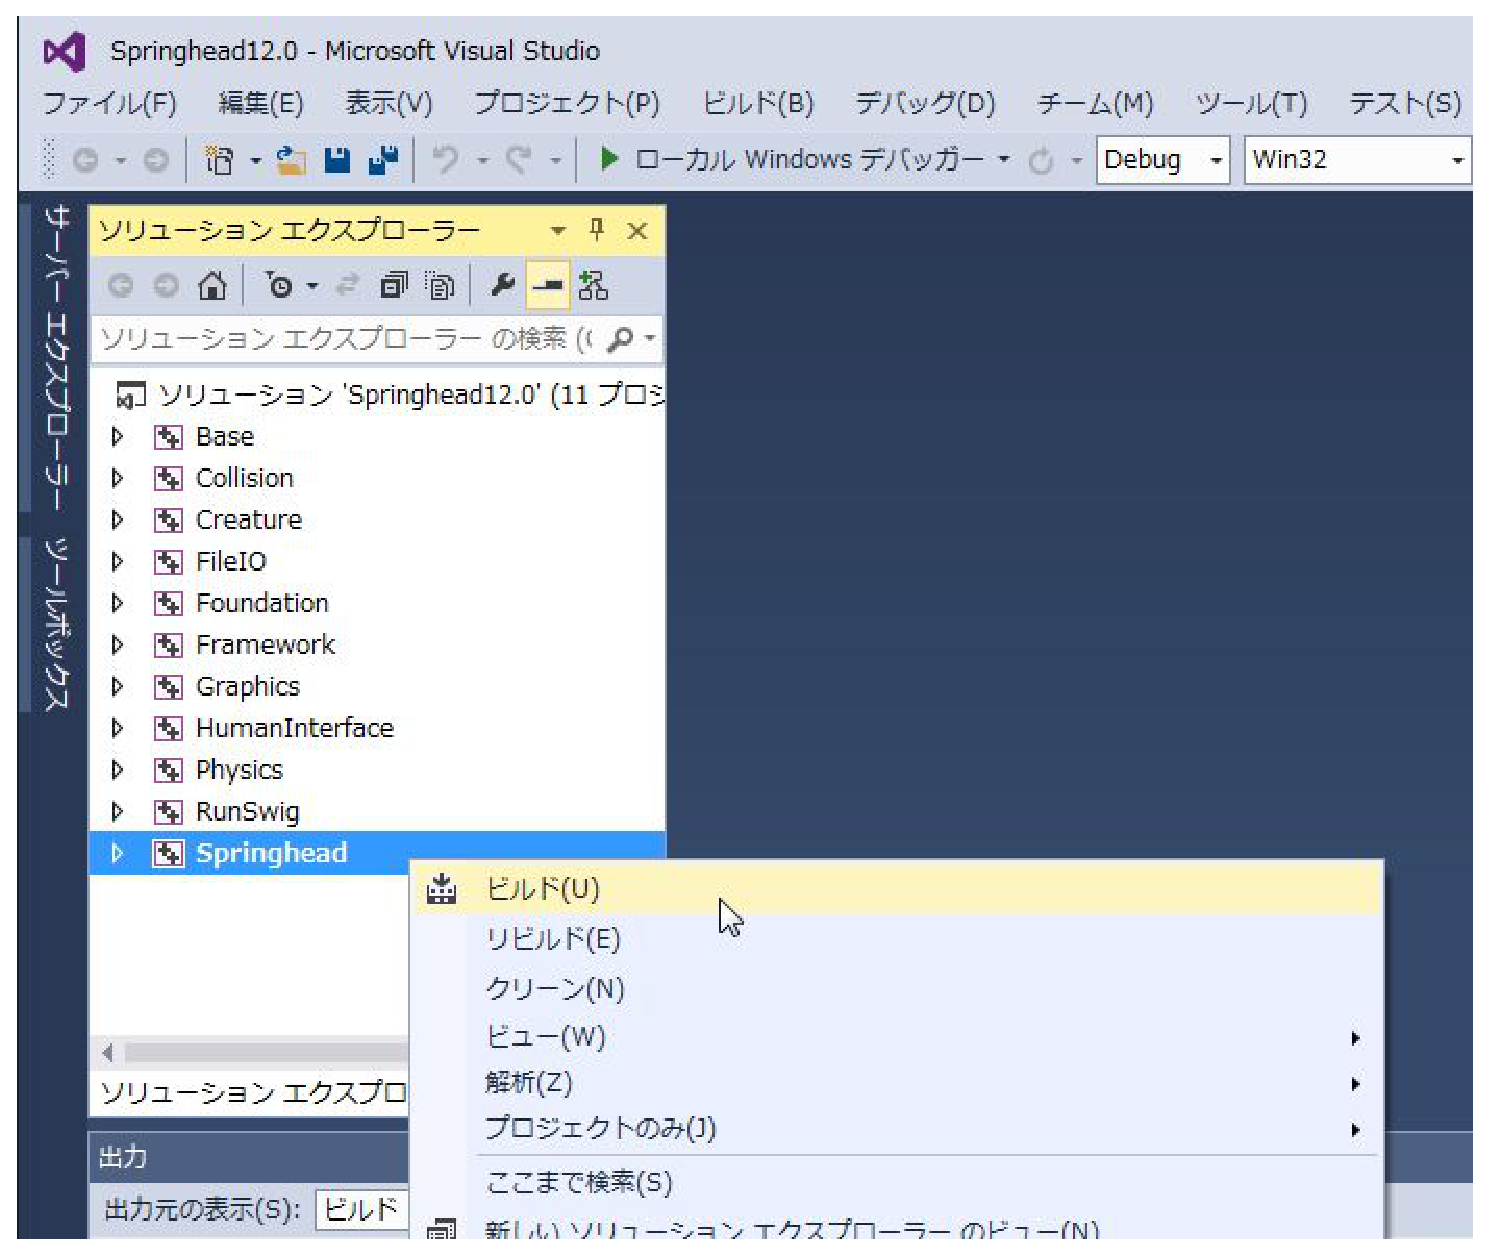
\includegraphics[width=.6\hsize]{fig/libbuild.eps}
\end{center}
\caption{Building the library}
\label{fig_libbuild}
\end{figure}
�\�����[�V�������J������Fig.\,\ref{fig_libbuild}�Ɏ����悤��
\url{Springhead}�v���W�F�N�g���r���h�����������D
�r���h�ɐ���������\path{C:\Springhead\generated\lib\win32\}
�܂���\path{C:\Springhead\generated\lib\win64\}
�f�B���N�g���Ƀ��C�u�����t�@�C�����쐬�����͂��ł��D

Table\,\ref{table_solution_config} �Ɏ����悤�ɁC
�r���h�̐ݒ育�ƂɈقȂ邢���‚��̍\�����p�ӂ���Ă��܂��D
���[�U�A�v���P�[�V�����̓s���ɍ��킹�Ďg�������Ă��������D

\begin{table}[t]
\caption{Build configurations}
\label{table_solution_config}
\begin{center}
\begin{tabular}{lll}
\toprule
�\����	      & �r���h�ݒ�		& �쐬����郉�C�u�����t�@�C���� \\ \midrule
\url{Release} & multithread, DLL	& \url{Springhead\# \#.lib}	 \\
\url{Debug}   & multithread, Debug, DLL	& \url{Springhead\# \#D.lib}	 \\
\url{Trace}   & multithread, Debug, DLL	& \url{Springhead\# \#T.lib}	 \\ \bottomrule
\multicolumn{3}{l}
{\footnotesize{%
\vbox{\vbox to 1mm{}
    \hbox{�E \url{\# \#}��Visual Studio�o�[�W������
	  �v���b�g�t�H�[����\��\url{Win32}����\url{x64}�̑g�ݍ��킹}
    \hbox{\phantom{�E }�ƂȂ�܂�("15.0x64" �Ȃ�)�D}
    \hbox{�E \url{Trace}�\���Ƃ́C�t���[���|�C���^���t��\url{Release}�\���̂��Ƃł��D}}}}
\end{tabular}
\end{center}
\end{table}

%\begin{center}\framebox{\small{%
%\begin{minipage}{0.9\hsize}
%�y�⑫�z ���C�u�����t�@�C���̃r���h�ݒ�y�і��̂͂���܂ł̊J���o�܂ɂ�闝�R�ŁC
%���X���G�ɂȂ��Ă��܂��D
%\begin{itemize}
%\item{Visual Studio 2008 �ł́C���ׂĂ̍\���� Static Link �ݒ�ł��D}
%\item{Visual Studio 2010 �ł́C \url{Release} / \url{Debug} �\���� Static Link �ݒ�,
%\url{ReleaseDll} / \url{DebugDll} / \url{Trace} �\���� DLL �ݒ�ł��D}
%\item{Visual Studio 2012 �ł́C���ׂĂ̍\���� DLL �ݒ�ł��D}
%\item{Visual Studio 2010 �ȑO�̃o�[�W�����ł́C�v���b�g�t�H�[���� 32�r�b�g�̏ꍇ�C���C�u�����t�@�C������ \url{Win32} ���t���܂���D}
%\item{Visual Studio 2010 �� \url{ReleaseDll} �\���y�� \url{DebugDll} �\���ł́C\url{.lib} �̑O�ɂ��ꂼ��
%\url{M} �y�� \url{MD} ���t���܂��D}
%\end{itemize}
%\end{minipage}
%}}\end{center}

\section{�T���v���v���O�����̃r���h}

�T���v���v���O�����́C\path{C:\Springhead\core\src\Samples}�ȉ��ɂ���܂��D
�c�O�Ȃ��Ƃł����C���ׂẴT���v���v���O���������Ȃ����삷���Ԃɂ͈ێ�����Ă��܂���D
\path{Physics\BoxStack}��\path{Physics\Joints}����r�I�ǂ������e�i���X����Ă��܂��̂�
�����Ă݂Ă��������D

�Ⴆ�΁C\path{Physics\BoxStack}���r���h����ɂ́C
\begin{align*}
\text{\path{C:\Springhead\core\src\Samples\Physics\BoxStack\ }}
\end{align*}
�Ɉړ�����\url{BoxStack15.0.sln}���J���܂��D
\url{BoxStack}���X�^�[�g�A�b�v�v���W�F�N�g�ɐݒ肵�C�r���h�C���s���Ă��������D

���s����DLL�����‚���Ȃ����߂ɃG���[���N���邩������܂���B���̏ꍇ�ɂ́C
32�r�b�g�‹��Ȃ��
\begin{align*}
\text{\path{Springhead\core\bin\win32}}, \text{\path{Springhead\dependency\bin\win32}}
\end{align*}
64�r�b�g�‹��Ȃ��
\begin{align*}
\text{\path{Springhead\core\bin\win64}}�C\text{\path{Springhead\dependency\bin\win64}}\\
\text{\path{Springhead\core\bin\win32}}�C\text{\path{Springhead\dependency\bin\win32}}
\end{align*}
�̂��ׂĂ�Path��ʂ��Ă��������B

\section{�A�v���P�[�V�����̍쐬}
\label{sec_create_application}

\begin{figure}[t]
\begin{center}
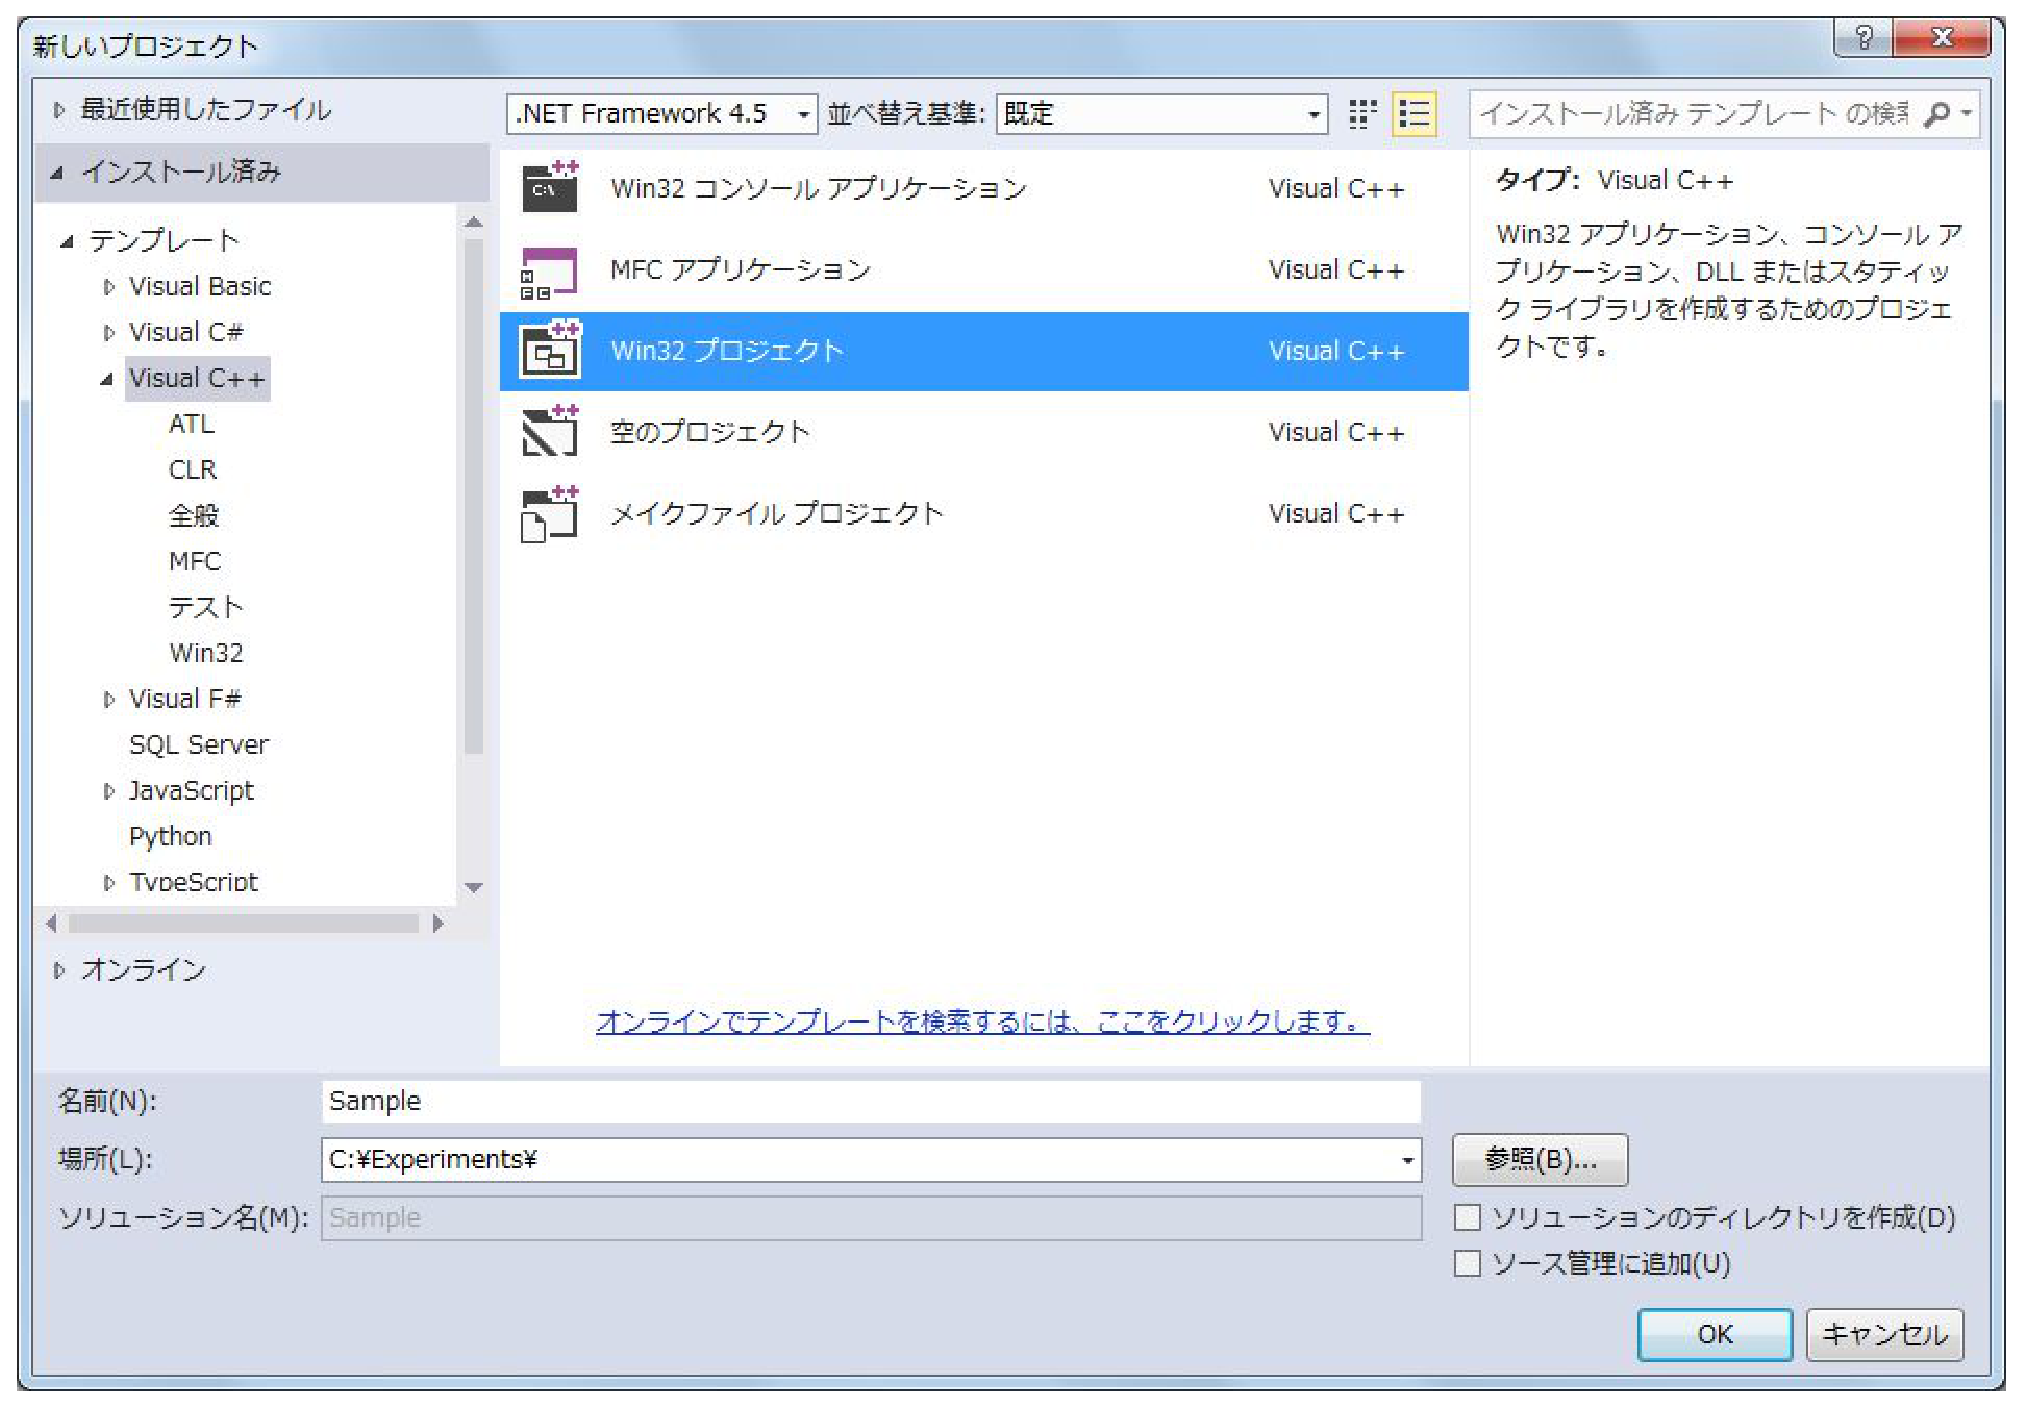
\includegraphics[width=.6\hsize]{fig/newproject1.eps}
\end{center}
\caption{Create new project}
\label{fig_newproject1}
\end{figure}

\begin{figure}[t]
\begin{center}
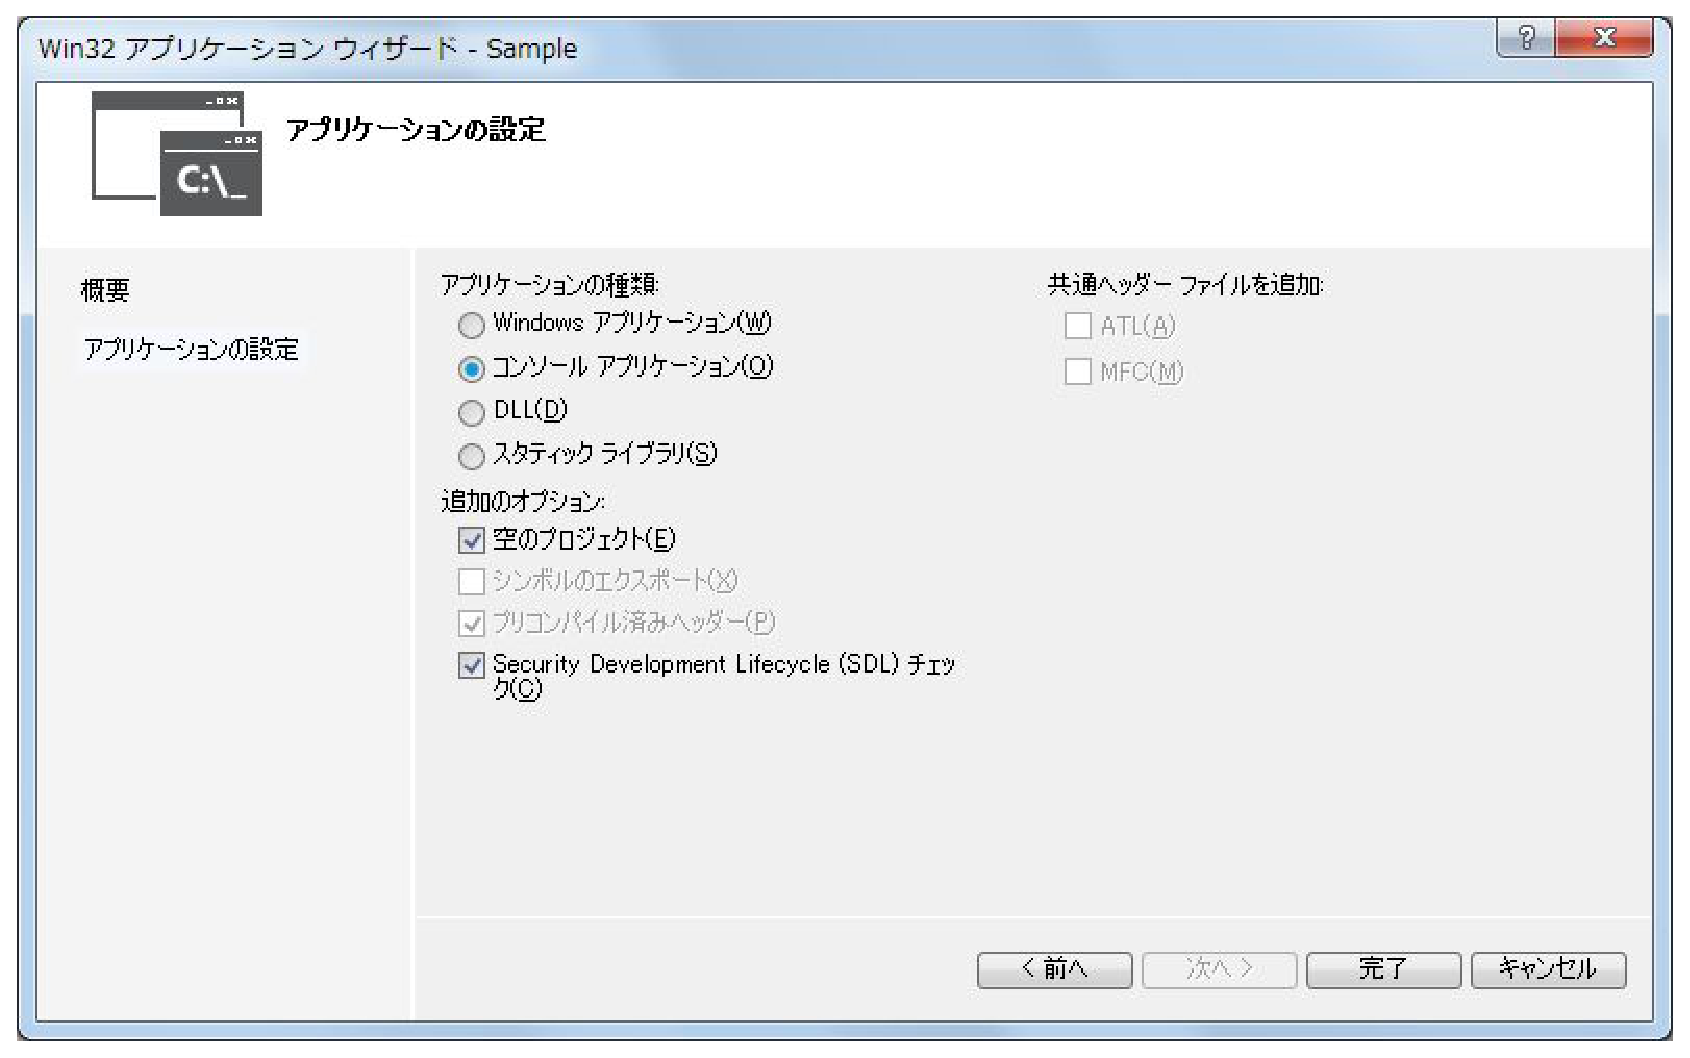
\includegraphics[width=.6\hsize]{fig/newproject2.eps}
\end{center}
\caption{Project configuration}
\label{fig_newproject2}
\end{figure}

\begin{figure}[t]
\begin{center}
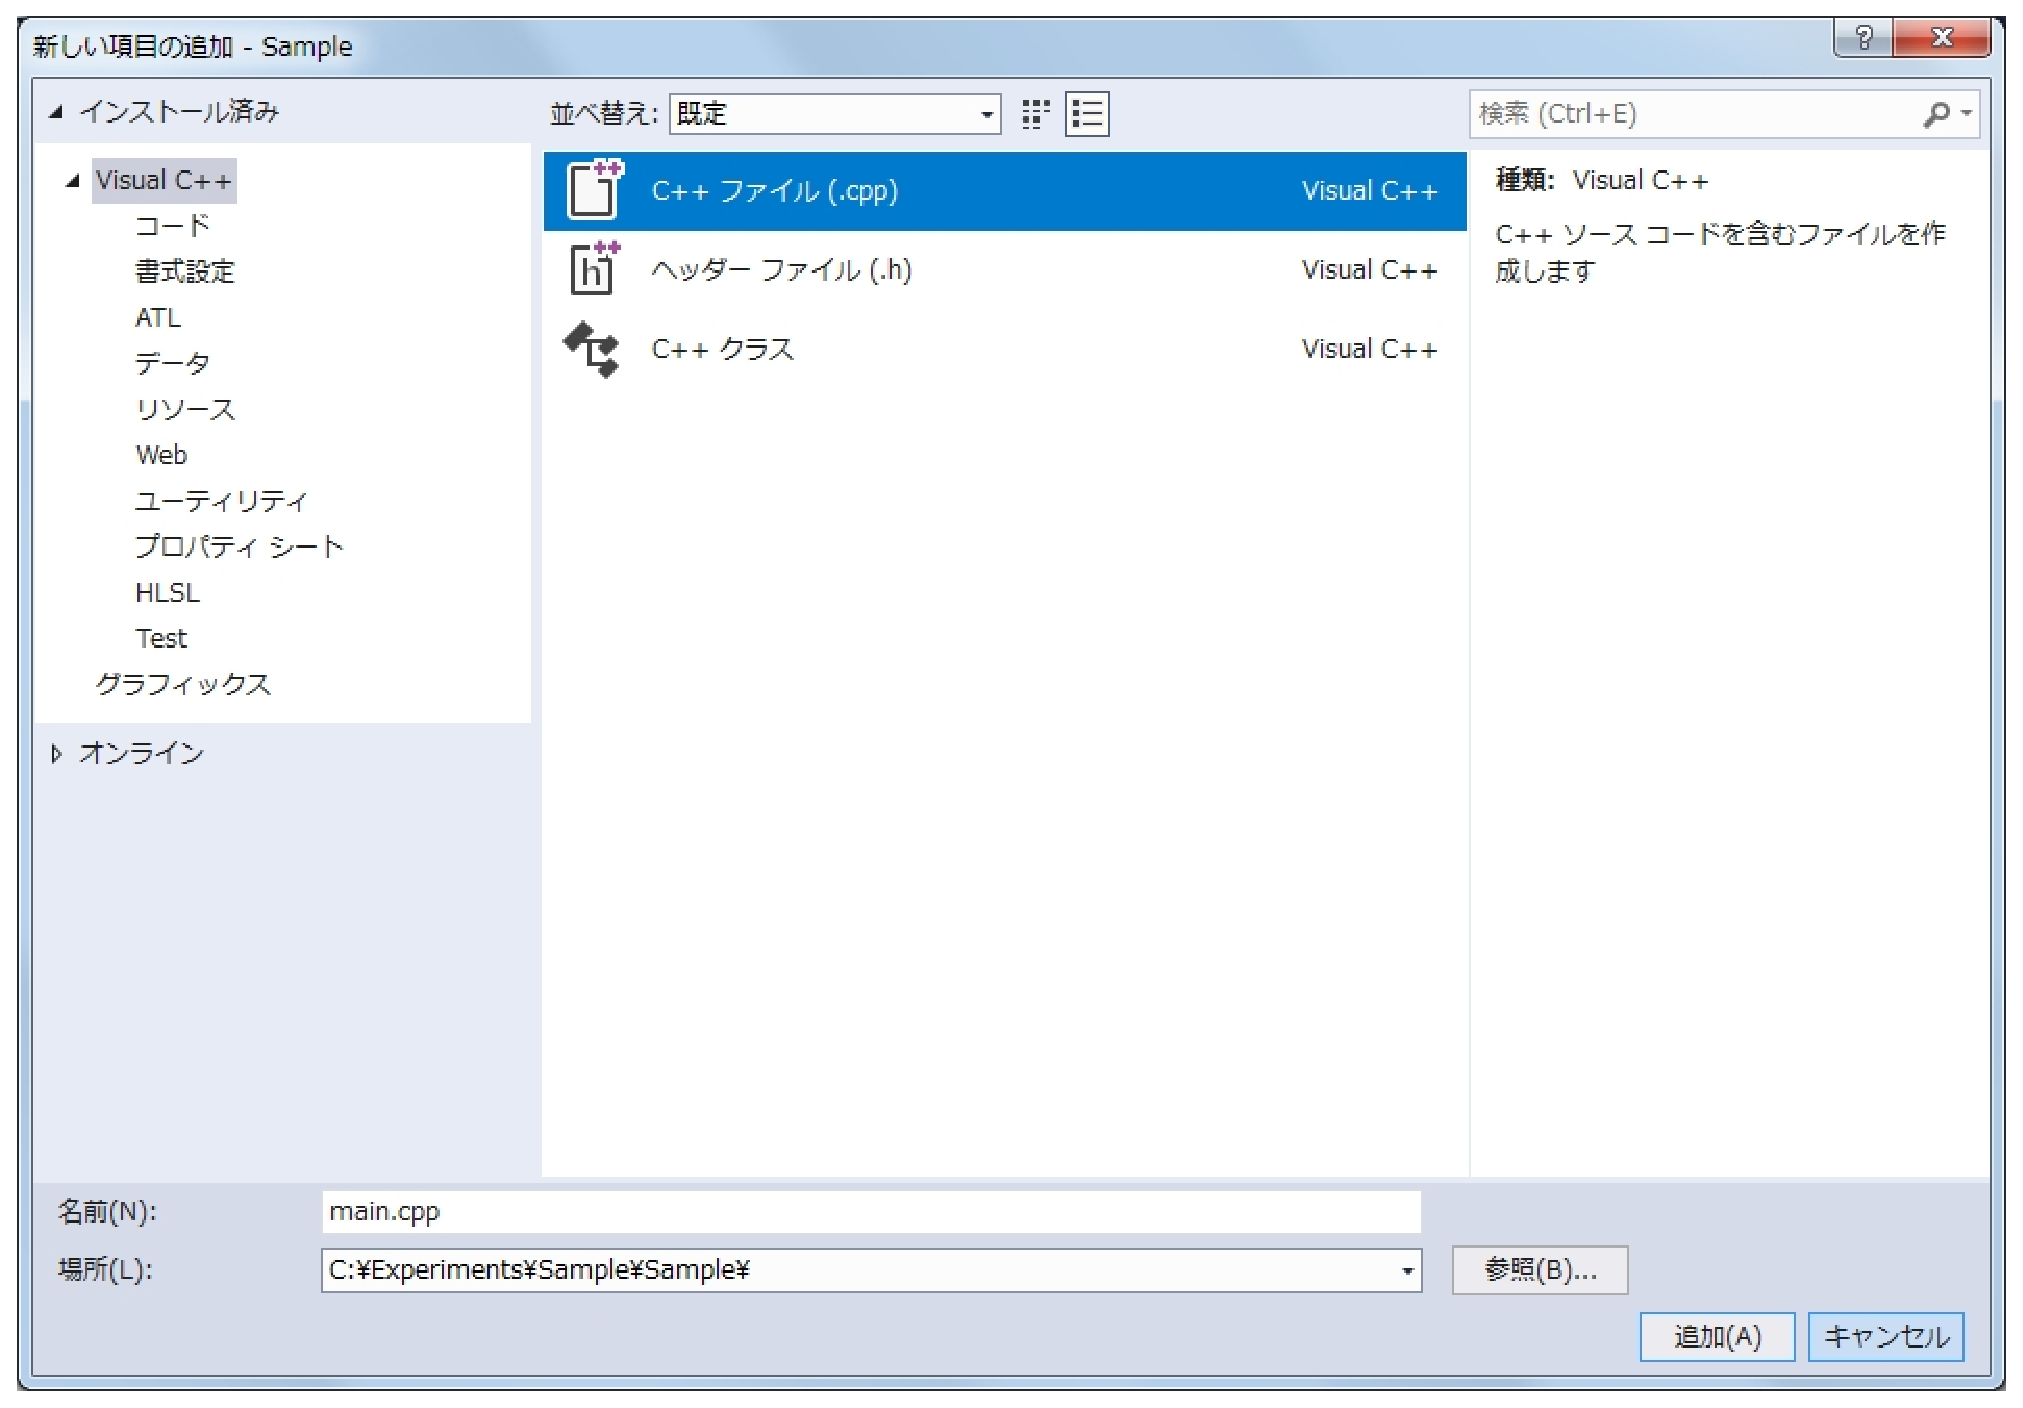
\includegraphics[width=.6\hsize]{fig/newproject3.eps}
\end{center}
\caption{Create source file}
\label{fig_newproject3}
\end{figure}

Springhead���g���ĊȒP�ȃA�v���P�[�V�����v���O�������쐬���铹�؂�������܂��D
�ȉ��ł�Visual Studio 2017��z�肵�܂��D

\subsection*{�v���W�F�N�g�̍쐬}

\newcommand{\RABra}{\raisebox{1pt}{ $>$ }}
�uVisual C++ Windows\RABra �f�X�N�g�b�v �E�B�U�[�h�v���쐬���܂��D
�쐬����f�B���N�g���� \path{C:\Experiments} �Ɖ��肵�܂��D
���̃f�B���N�g���ɍ쐬����ꍇ�ɂ́C
�v���W�F�N�g�Ɏw�肷��C���N���[�h�t�@�C���y�у��C�u�����t�@�C���̃p�X���C
�ۑ�����Springhead�𐳂����Q�Ƃ���悤�ɒ��ӂ��Ă��������D
�v���W�F�N�g���͍D���Ȗ��O��t���Ă��������D
�A�v���P�[�V�����̐ݒ�Łu�R���\�[���A�v���P�[�V�����v��I�сC
��̃v���W�F�N�g���`�F�b�N���܂��D

\begin{center}\framebox{\small{%
\begin{minipage}{0.9\hsize}
�y�⑫�z Visual Studio 2015���g�p�����ꍇ�A
Fig.\,\ref{fig_newproject1}�AFig.\,\ref{fig_newproject2}�Ƃ�
�قȂ�E�B���h�E���\������܂��B
���̏ꍇ�ɂ́uWin32�v���W�F�N�g\RABra ���ցv�Ɛi��ŁA
�u�R���\�[���A�v���P�[�V�����v�A�u��̃v���W�F�N�g�v���`�F�b�N���܂��B
\end{minipage}
}}\end{center}

�v���W�F�N�g���쐬������
�u�v���W�F�N�g\RABra �V�������ڂ̒lj�\RABra C++�t�@�C��(.cpp)�v
�Ƃ��ă\�[�X�t�@�C�����쐬���܂��D
�����ł͉���\url{main.cpp}�Ƃ��܂��D

\subsection*{�\�[�X�R�[�h�̕ҏW}

\begin{table}[t]
\caption{Simplest program code}
\label{table_simplest_code}
{\small
\begin{sourcecode}
#include <Springhead.h>
#include <Framework/SprFWApp.h>
using namespace Spr;

class MyApp : public FWApp{
public:
    virtual void Init(int argc = 0, char* argv[] = 0){
        FWApp::Init(argc, argv);

        PHSdkIf* phSdk = GetSdk()->GetPHSdk();
        PHSceneIf* phscene = GetSdk()->GetScene()->GetPHScene();
        CDBoxDesc bd;
        
        // �����쐬
        PHSolidIf* floor = phscene->CreateSolid();
        floor->SetDynamical(false);
        bd.boxsize = Vec3f(5.0f, 1.0f, 5.0f);
        floor->AddShape(phSdk->CreateShape(bd));
        floor->SetFramePosition(Vec3d(0, -1.0, 0));
    
        // �����쐬
        PHSolidIf* box = phscene->CreateSolid();
        bd.boxsize = Vec3f(0.2f, 0.2f, 0.2f);
        box->AddShape(phSdk->CreateShape(bd));
        box->SetFramePosition(Vec3d(0.0, 1.0, 0.0));

        GetSdk()->SetDebugMode(true);
    }
} app;

int main(int argc, char* argv[]){
    app.Init(argc, argv);
    app.StartMainLoop();
    return 0;
}
\end{sourcecode}
}
\end{table}

�쐬����\url{main.cpp}��
Table\,\ref{table_simplest_code}�Ɏ����R�[�h����������ł��������D
���ꂪSpringhead���g�p���� (�ق�) �ŏ��̃v���O�����R�[�h�ł��D

\section*{�v���W�F�N�g�ݒ�}

\begin{figure}[t]
\begin{center}
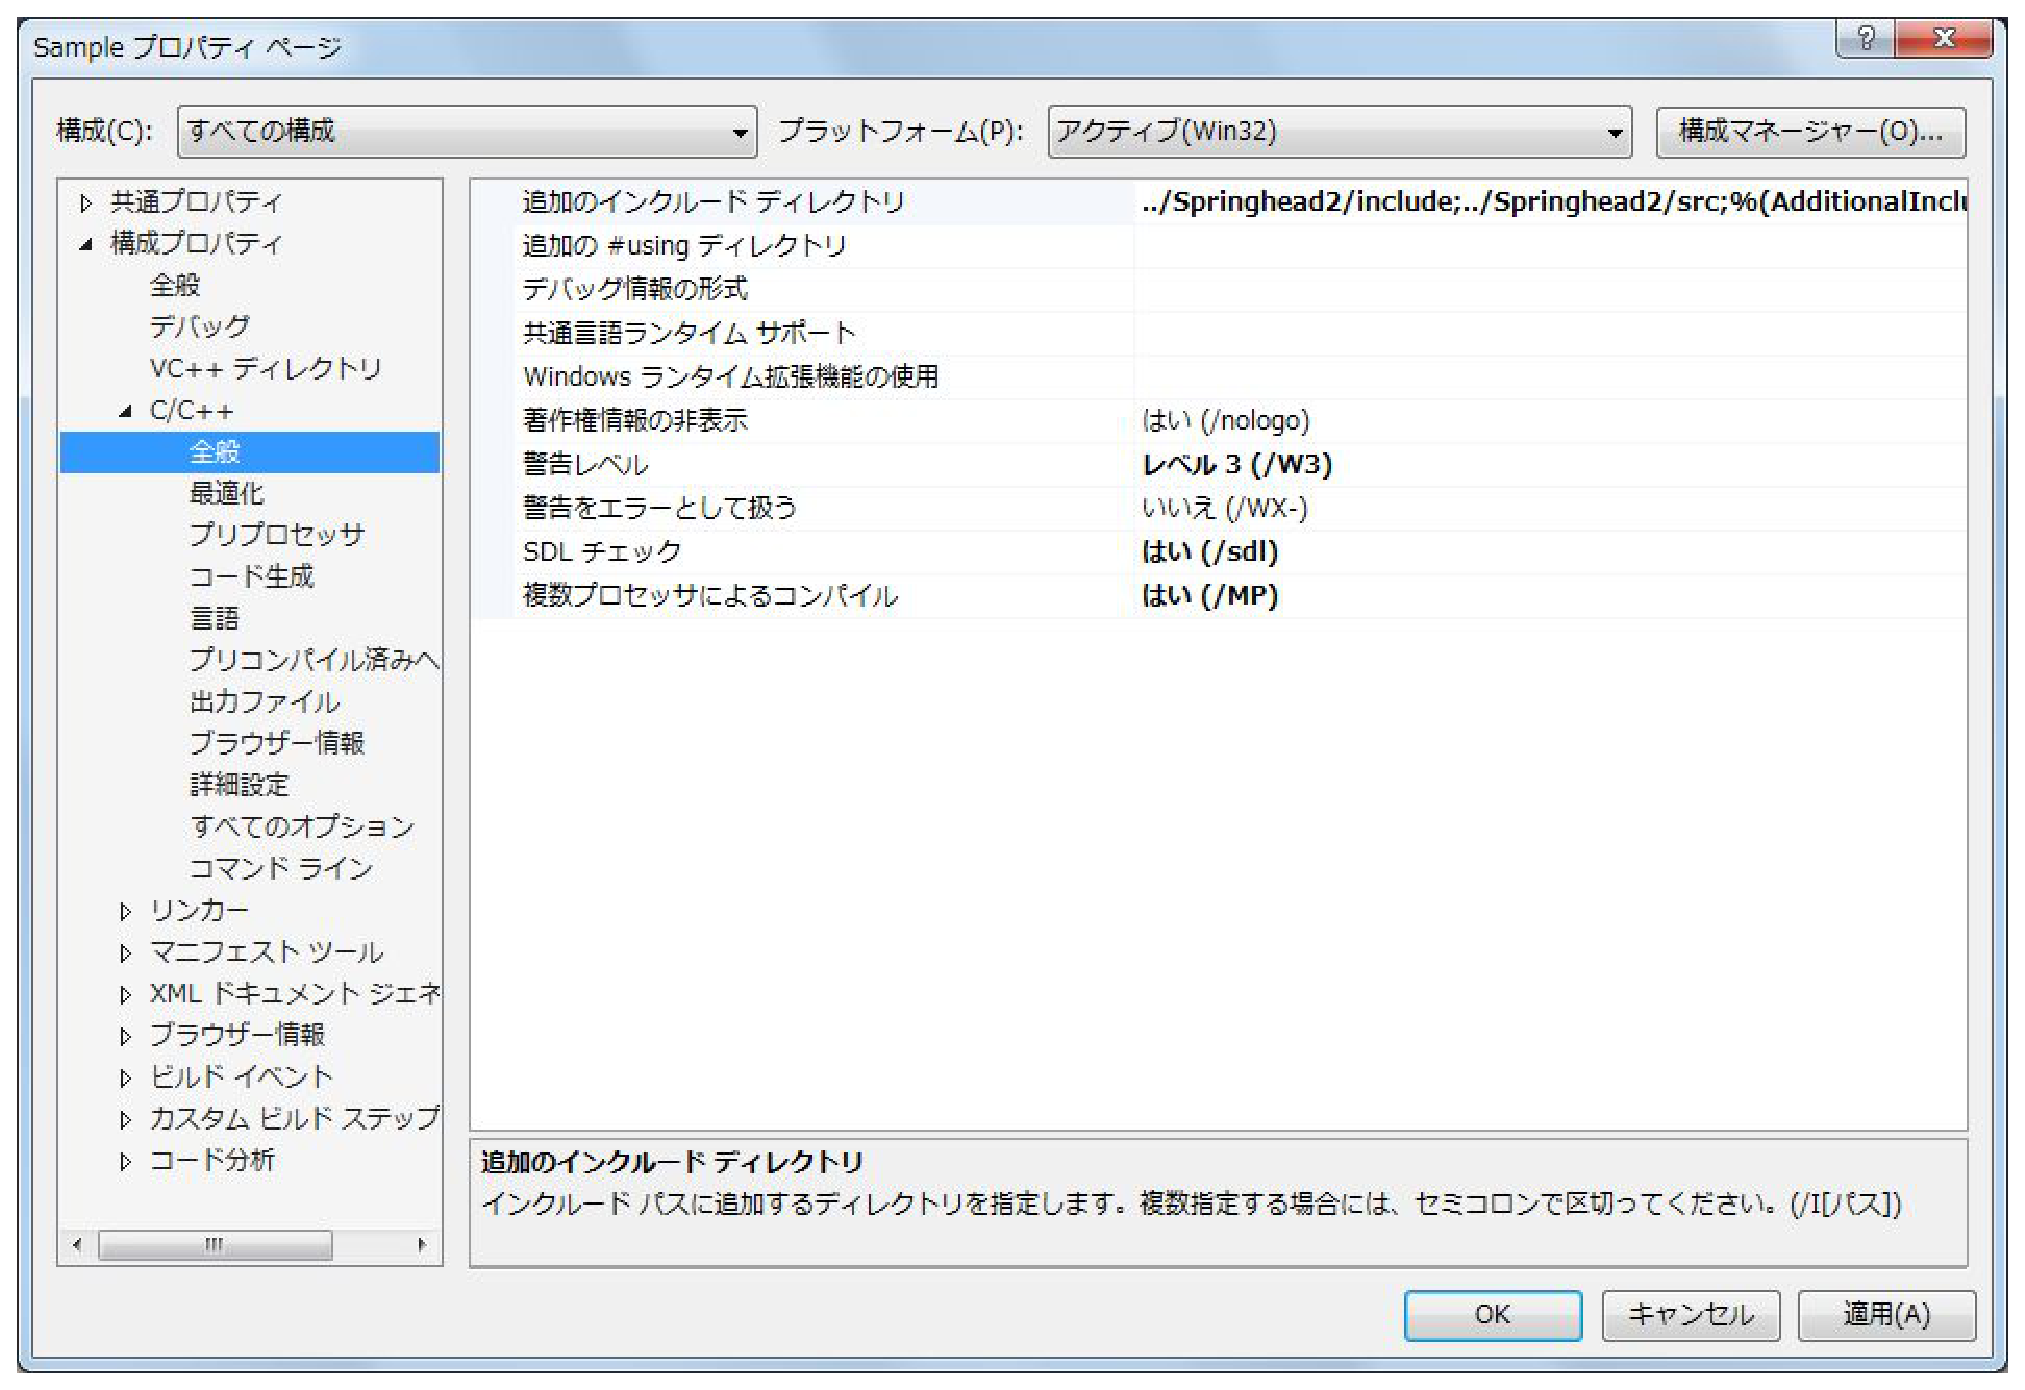
\includegraphics[width=.6\hsize]{fig/newproject4.eps}
\end{center}
\caption{Add include path}
\label{fig_newproject4}
\end{figure}

\begin{figure}[t]
\begin{center}
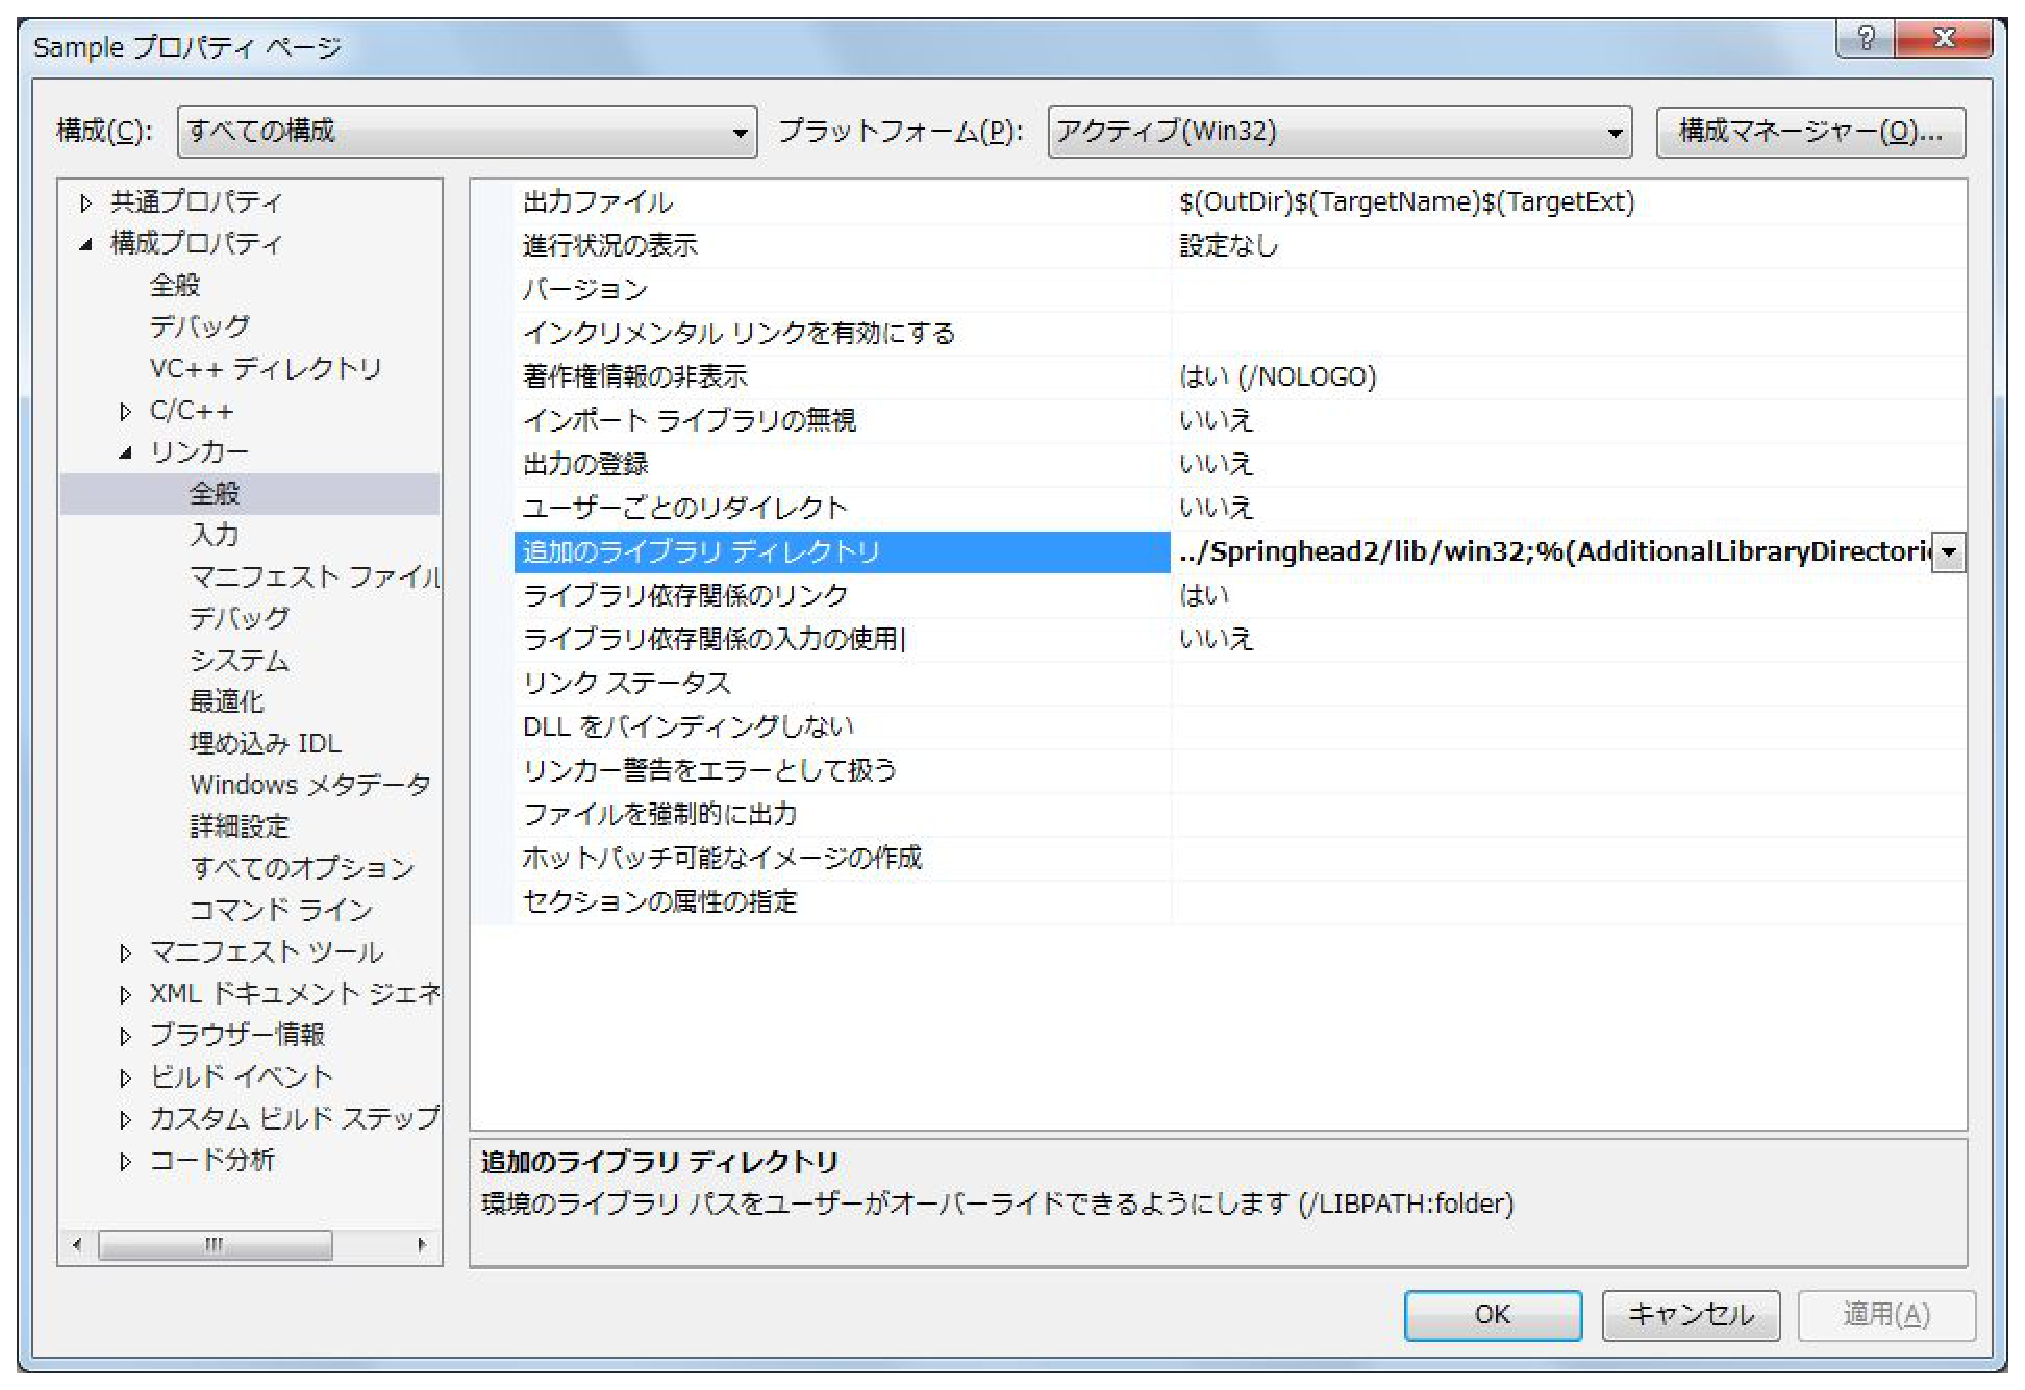
\includegraphics[width=.6\hsize]{fig/newproject5.eps}
\end{center}
\caption{Add library path}
\label{fig_newproject5}
\end{figure}

\begin{figure}[t]
\begin{center}
\begin{tabular}{c}
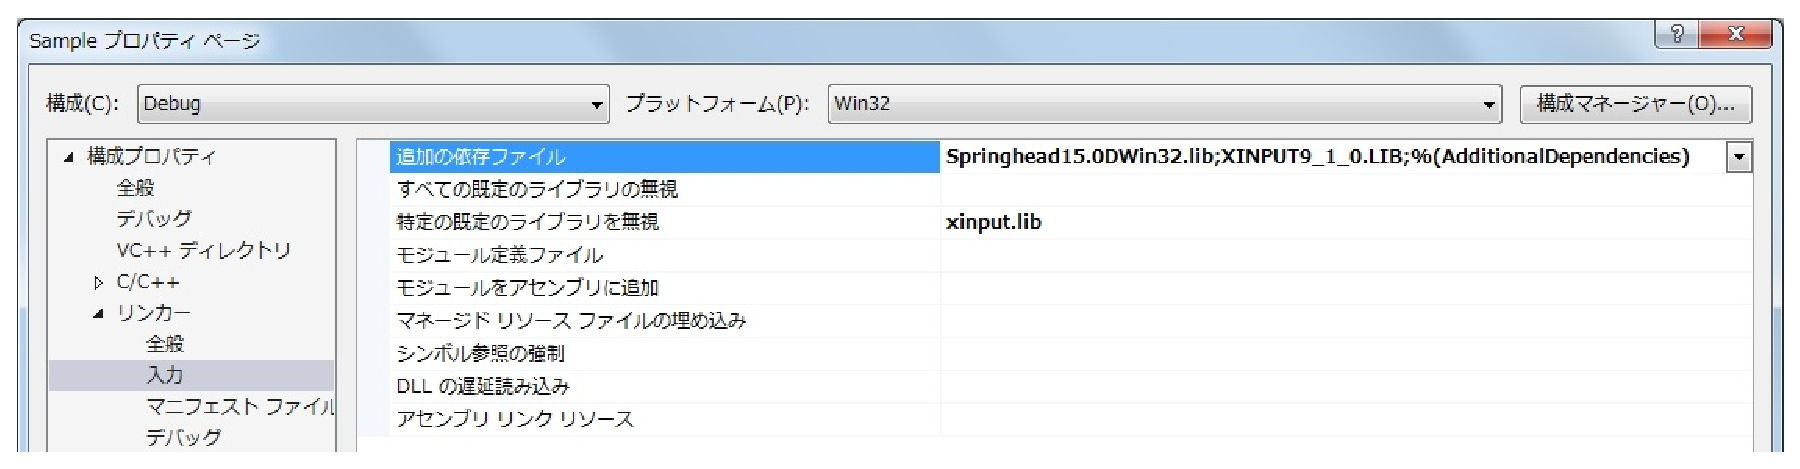
\includegraphics[width=.6\hsize]{fig/newproject6_truncate.eps} \\
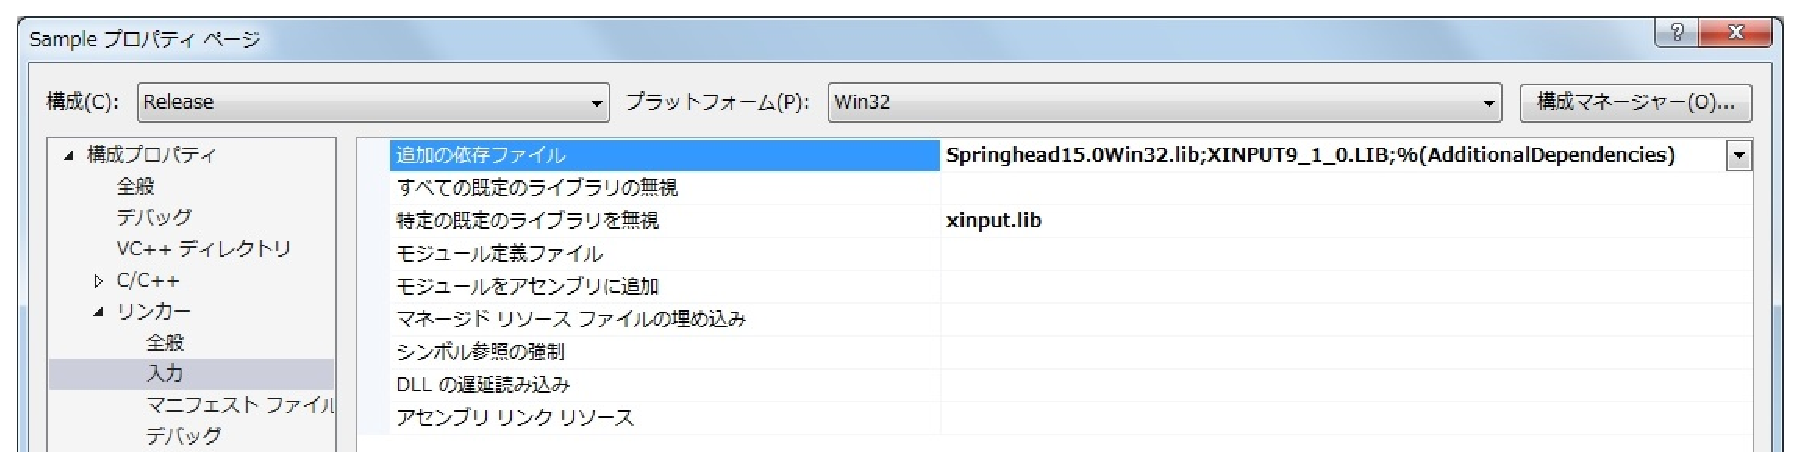
\includegraphics[width=.6\hsize]{fig/newproject7_truncate.eps}
\end{tabular}
\end{center}
\caption{Specify library file}
\label{fig_newproject6}
\end{figure}

\begin{figure}[t]
\begin{center}
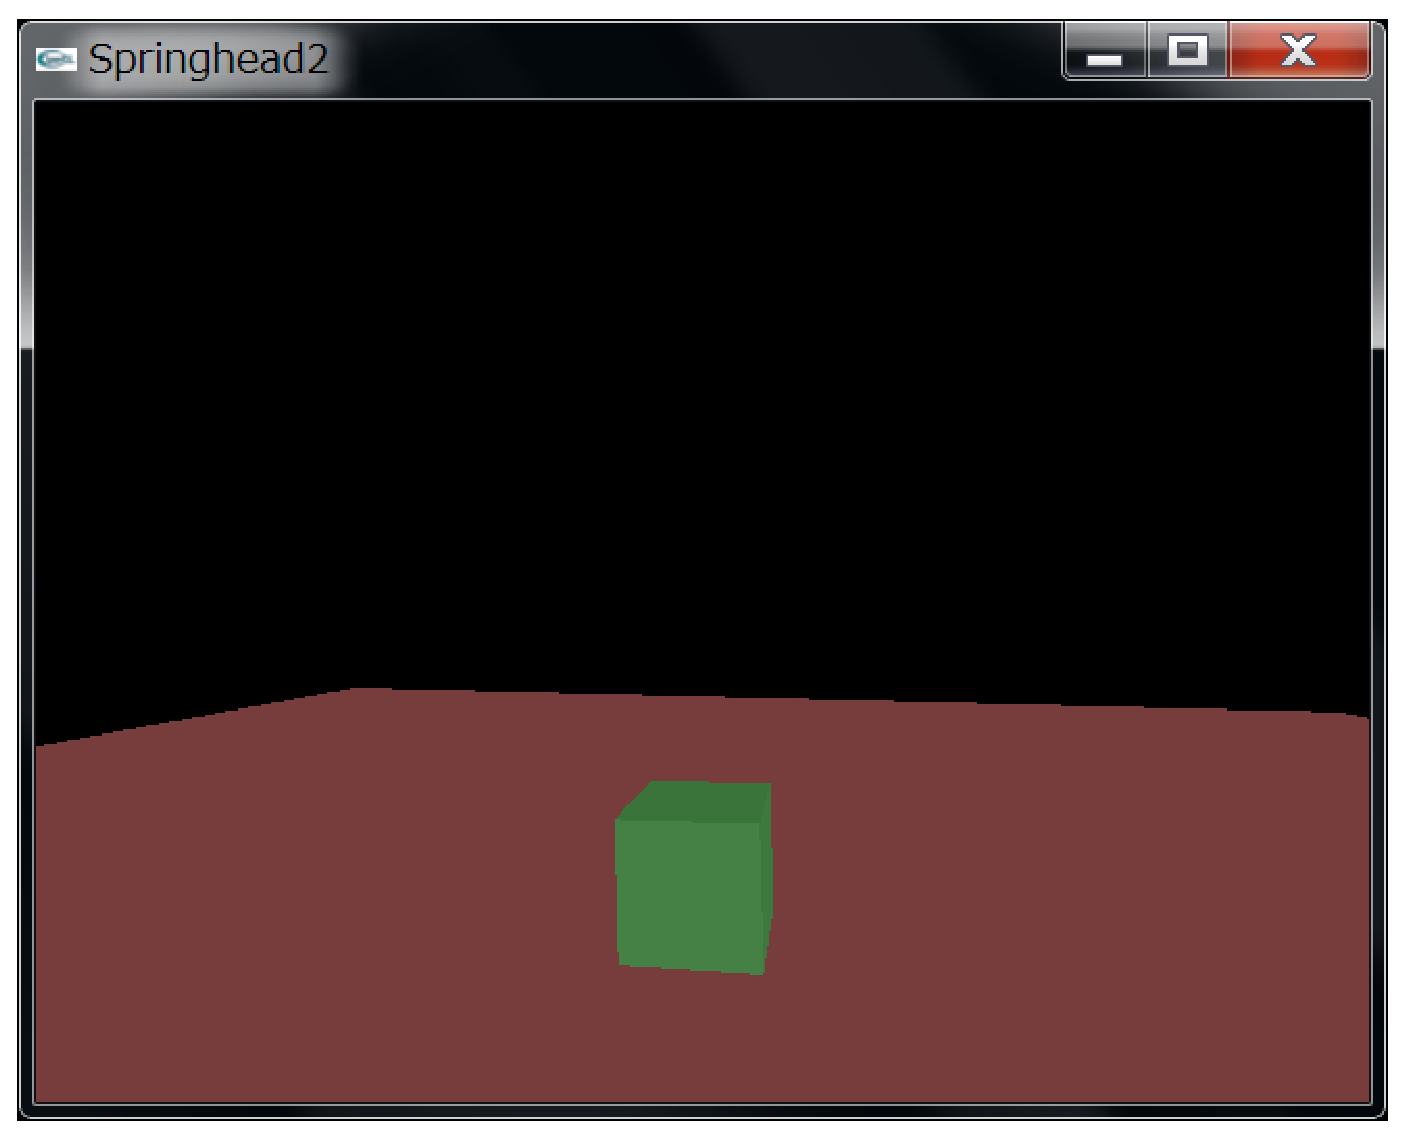
\includegraphics[width=.6\hsize]{fig/newproject8.eps}
\end{center}
\caption{Program running}
\label{fig_newproject8}
\end{figure}

�r���h����܂��ɂ����‚��̃v���W�F�N�g�ݒ肪�K�v�ł��D
64�r�b�g�v���b�g�t�H�[�����g�p����ꍇ�ɂ́C
�v���p�e�B�[�y�[�W�́u�\���}�l�[�W���[�v��
�u\url{x64}�v�v���b�g�t�H�[����V�K�쐬���đI�����Ă����܂��D
�܂��C\ref{libbuild} �Ő����������C�u�����̃r���h�͍ς�ł�����̂Ƃ��܂��D

�܂��v���W�F�N�g�̃v���p�e�B�y�[�W���J���C�\�����u���ׂĂ̍\���v�Ƃ��Ă��������D
���ɁuC/C++\RABra �S��\RABra �lj��̃C���N���[�h�f�B���N�g���v�ɁC
Fig.\,\ref{fig_newproject4}�̂悤��
Springhead�̃C���N���[�h�t�@�C���ւ̃p�X���w�肵�Ă��������D
����ɁC�u�����J�[\RABra �S��\RABra �lj��̃��C�u�����f�B���N�g���v��
Fig.\,\ref{fig_newproject5}�̂悤��Springhead�̃��C�u�����t�@�C���ւ̃p�X���w�肵�܂�
(64�r�b�g�\���̏ꍇ��\url{win32}�̑����\url{win64}���w�肵�܂�)�D

���x�͍\�����uDebug�v�ɂ��܂��D
�uC/C++\RABra �R�[�h����\RABra �����^�C�����C�u�����v��
�u�}���`�X���b�h �f�o�b�O DLL(\url{/MDd})�v�ɂ��܂��D
���Ɂu�����J�[\RABra ����\RABra �lj��̈ˑ��t�@�C���v��
\url{Springhead15.0DWin32.lib} (�܂���\url{Springhead15.0Dx64.lib})��lj����Ă��������D

�Ō�ɍ\�����uRelease�v�ɐ؂�ւ��ē��l�̐ݒ�����܂��D
�����^�C�����C�u�������u�}���`�X���b�h DLL(\url{/MD})�v�Ƃ��āC
�lj��̈ˑ��t�@�C����
\url{Springhead15.0Win32.lib} (�܂���\url{Springhead15.0Dx64.lib})��lj����܂��D

\section*{�r���h�E���s}

�ȏ�ŏ��������ł��D�r���h(F7)���āC���s(F5)���Ă݂Ă��������D
Fig.\,\ref{fig_newproject8}�̂悤�ȉ�ʂ��o�Ă���ΐ����ł��D


\chapter{Springhead�̍\��}
\label{chap_structure}
\section{�f�B���N�g���\��}

\begin{figure}[t]
\begin{center}
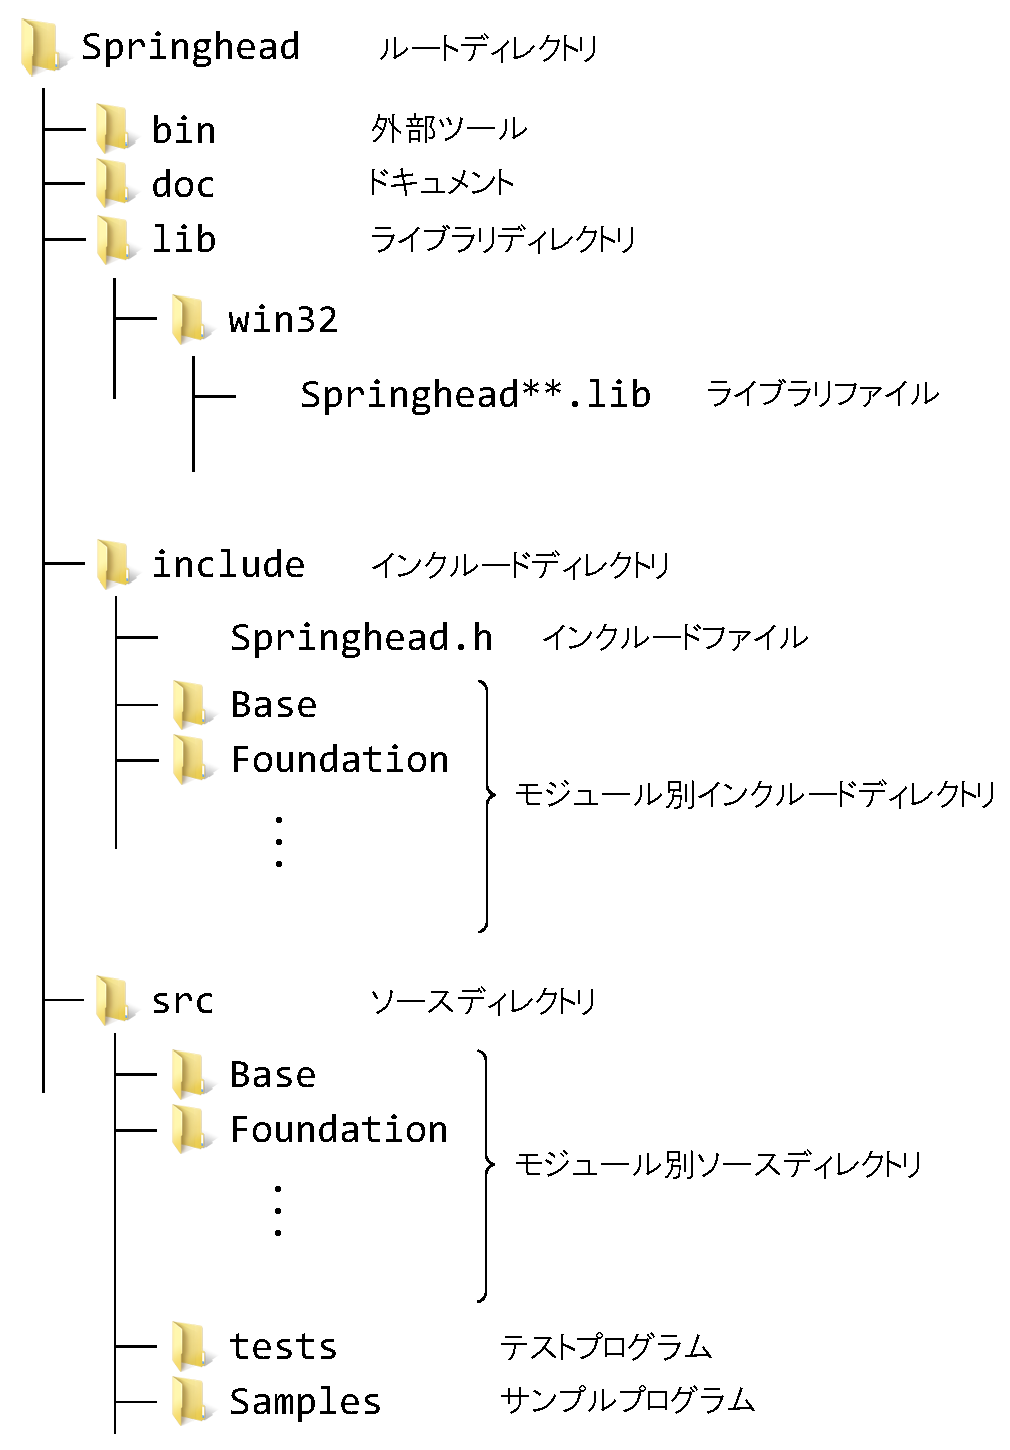
\includegraphics[width=.6\hsize]{../fig/filetree.eps}
\end{center}
\caption{Directory tree of Springhead}
\label{fig_filetree}
\end{figure}

Springhead�̃f�B���N�g���\����Fig.\,\ref{fig_filetree}�Ɏ����܂��D

\section{���C�u�����\��}

\begin{table}[t]
\caption{Springhead modules}
\label{table_modules}
\begin{tabular}{lll}
\toprule
���W���[����			& �v���t�B�b�N�X	& �@�\	\\ \midrule
{\bf Base}				& -					& �s��E�x�N�g�����Z�C�X�}�[�g�|�C���^�C\\
						&					& ���̑���{�@�\	\\
{\bf Foundation}		& UT				& Springhead�̊�{�N���X�C���s���^���	\\
{\bf Collision}			& CD				& �Փ˔���	\\
{\bf Physics}			& PH				& �����v�Z	\\
{\bf Graphics}			& GR				& �V�[���O���t�C�`��	\\
{\bf FileIO}			& FI				& �t�@�C�����o��	\\
{\bf HumanInterface}	& HI				& �q���[�}���C���^�t�F�[�X�f�o�C�X�� \\
						&					& �C���^���N�V���� \\ 
{\bf Creature}			& CR				& �o�[�`�����N���[�`�� \\
{\bf Framework}			& FW				& ���W���[���Ԃ̘A�g�� \\
						&					& �A�v���P�[�V�����쐬�x�� \\ \bottomrule
\end{tabular}
\end{table}

\begin{table}[t]
\caption{Module dependencies}
\label{table_dependency}
\begin{center}
\begin{tabular}{llllllllll}
\toprule
���W���[����			& 			&			&			&			&			&			&			&			&			\\ \midrule
{\bf Base}				& -			& -			& -			& -			& -			& -			& -			& -			& -			\\
{\bf Foundation}		& $\circ$	& -			& -			& -			& -			& -			& -			& -			& -			\\
{\bf Collision}			& $\circ$	& $\circ$	& -			& -			& -			& -			& -			& -			& -			\\
{\bf Physics}			& $\circ$	& $\circ$	& $\circ$	& -			& -			& -			& -			& -			& -			\\
{\bf Graphics}			& $\circ$	& $\circ$	& -			& -			& -			& -			& -			& -			& -			\\
{\bf FileIO}			& $\circ$	& $\circ$	& -			& -			& -			& -			& -			& -			& -			\\
{\bf HumanInterface}	& $\circ$	& $\circ$	& -			& -			& -			& -			& -			& -			& -			\\
{\bf Creature}			& $\circ$	& $\circ$	& -			& $\circ$	& -			& -			& -			& -			& -			\\
{\bf Framework}			& $\circ$	& $\circ$	& -			& $\circ$	& $\circ$	& $\circ$	& $\circ$	& -			& -			\\ \bottomrule
\end{tabular}
\end{center}
\end{table}

Springhead�͕����̃��W���[������\������Ă��܂��D
Table\,\ref{table_modules}�Ƀ��W���[���ꗗ�������܂��D
Table\,\ref{table_dependency}�Ƀ��W���[���Ԃ̈ˑ��֌W�������܂��D
�ʏ�C���[�U��Springhead���g�p����ɂ������Ă����̈ˑ��֌W��z�Ɉӎ�����K�v�͂���܂���D
�܂��C���炩�̎����Springhead�̓���̋@�\�i���Ƃ��Ε����V�~�����[�V�����j�݂̂�p�������Ƃ����ꍇ�ɑΉ��ł���悤�ɁC
���W���[���Ԃ̈ˑ��֌W�͂Ȃ�ׂ��a�ɂȂ�悤�ɐ݌v����Ă��܂��D
���������Ă��̂悤�ȏꍇ�ɂ͗p�r�ɉ����ĕK�v�ȃ��W���[���݂̂��g����悤�ɂȂ��Ă��܂��D

\section{�N���X�EAPI�̖����K��}

�e���W���[���Ɋ܂܂��N���X�̖��O�ɂ́CTable\,\ref{table_modules}�Ɏ������悤�ȃ��W���[���ŗL�̃v���t�B�b�N�X���‚��܂�
(��: Physics���W���[����\texttt{PHSolid}�CCollision���W���[����\texttt{CDShape})�D
�ꕔ�ɂ͂��̃��[���ɂ�������Ȃ��N���X�����݂��܂�(��: Foundation���W���[����Object)�D

API(�N���X�̃����o�֐�)�ɂ��ɂ������K��������܂��D
API���͊�{�I��(���� + �ړI��)�Ƃ����`���ŏ������e��[�I�ɕ\�����܂��D
�܂��C�P��̐擪�����̂ݑ啶���C���̑��͏������ŕ\�L���܂��D
��Ƃ��Ă�\texttt{PHSolid::SetMass}�C\texttt{GRSdk::CreateScene}�Ȃǂł��D

\section{�C���^�t�F�[�X�ƃf�B�X�N���v�^} 
\label{section_if_desc}

Springhead�ł͎d�l�Ǝ����𖾊m�ɕ������邽�߂ɁC�C���^�t�F�[�X�N���X�Ǝ����N���X���������Ă��܂��D
���[�U�̓C���^�t�F�[�X�N���X�݂̂��g�p����Springhead�̋@�\�𗘗p���܂��D
�������C\url{Base}��\url{Foundation}���W���[���ɂ��邲����{�I�ȃN���X�C�����\url{Framework}�̃A�v���P�[�V�����N���X�͗�O�ƂȂ��Ă��܂��D

�܂��CSpringhead�̃N���X�ɂ͂��ꂼ��Ƀf�B�X�N���v�^���p�ӂ���Ă��܂��D�f�B�X�N���v�^�Ƃ́C���̃N���X�̓ǂݏ����”\�ȑ����݂̂��W�߂��\���̂ł��D
�f�B�X�N���v�^�𗘗p���邱�ƂŁC�����ݒ�̃C���X�^���X�𑽐��ݒ肷�邱�Ƃ��p�ӂɂȂ�܂��D
�܂��C�f�B�X�N���v�^�̓t�@�C���ւ̃f�[�^�̕ۑ���ǂݍ��݂ɂ����Ă��𗧂��܂��D

�ȉ���\url{Physics}���W���[���̍��̂�\��\url{PHSolid}�N���X���ɂƂ��Đ������܂��D
\begin{sourcecode}
// given PHSolidIf* phScene, 

PHSolidDesc desc;
desc.mass = 1.0;

PHSolidIf* solid = phScene->CreateSolid(desc);
\end{sourcecode}
��̃R�[�h��\url{PHSolidDesc}��\url{PHSolid}�N���X�̃f�B�X�N���v�^�ł��D
�܂����̃����o�ϐ�\url{mass}�ɒl���Z�b�g���邱�Ƃō��̂̎��ʂ�ݒ肵�Ă��܂��D
���ɁC���̂��쐬���邽�߂�\url{CreateSolid}�֐����Ă΂�܂��D
������\url{CreateSolid}�͕����V�[����\��\url{PHScene}�N���X�̃����o�֐��ł��D
���ۂɂ�\url{PHScene}�N���X�̃C���^�t�F�[�X\url{PHSceneIf}���擾����K�v������܂����C�����ł͊��ɓ����Ă���Ƃ��Ă��܂��D
���̂��쐬�����ƁC\url{CreateSolid}����C���^�t�F�[�X\url{PHSolidIf}�̃|�C���^���Ԃ���܂��D
����ȍ~�̍��̂̑���͂��̃C���^�t�F�[�X����čs���܂��D
\begin{sourcecode}
solid->SetMass(5.0);
\end{sourcecode}
��{�I�ɁC�f�B�X���v�^����Đݒ�”\�ȑ����̓C���^�t�F�[�X��\url{Get/Set}�n�֐����g���Ď擾�C�ݒ肪�ł���悤�ɂȂ��Ă��܂��D
�ꍇ�ɉ����ĕ֗��ȕ����g���Ă��������D

Springhead�I�u�W�F�N�g�͂��ׂē����Ń������Ǘ�����Ă��܂��̂ŁC���[�U�������I��\url{delete}����K�v�͂���܂���i�܂��C���Ă͂����܂���j�D
\url{Create}���ꂽ�I�u�W�F�N�g�̓v���O�����̏I�����Ɏ����I�ɔj������܂��D

\section*{���ڂ����m�肽���l��}

�ȍ~�̏͂ł͊e���W���[���ɂ‚��Ă��ڂ����������܂��D
Springhead�𗘗p�����ŁC���ׂẴ��W���[�����ڂ�����������K�v�͂���܂���D
�K�v�ɉ����ĎQ�Ƃ��Ă��������D


\chapter{Base}
\label{chap_base}
Base\index{Base}Module is a composition of basic functions.

\section{Matrices and vectors operation}

\begin{table}[t]
\caption{Matrix and vector classes}
\label{table_matrix}
\begin{center}
\begin{tabular}{ll}
\toprule
Classname							& Role 					\\ \midrule
\texttt{Vec[2|3|4][f|d]}			& Vector				\\
\texttt{Matrix[2|3|4][f|d]}			& Matrix				\\
\texttt{Quaternion[f|d]}			& Unit quaternion		\\
\texttt{Affine[f|d]}				& Affine transform		\\
\texttt{Pose[f|d]}					& Composition of a three-dimensional vector and a quaternion \\
\bottomrule
\end{tabular}
\end{center}
\end{table}

Table\,\ref{table_matrix} shows frequently used vector and matrix classes.
Suffix integers represent size of vector and matrix. 
\texttt{f} and \texttt{d} correspons \texttt{float}type and \texttt{double}type respectively.

\subsection*{�x�N�g��}

\index{Vec2f}\index{Vec3f}\index{Vec4f}
\index{Vec2d}\index{Vec3d}\index{Vec4d}
\index{�ׂ��Ƃ�@�x�N�g��}

�x�N�g���^�͕��̂̈ʒu�⑬�x�C�͂Ȃǂ̕����ʂ�\�����邽�߂ɕp�ɂɎg���܂��D
�Ⴆ��\texttt{double}�^�̗v�f����Ȃ�3�����x�N�g��\texttt{x}���`����ɂ�
\begin{sourcecode}
Vec3d x;
\end{sourcecode}
�Ƃ��܂��D�v�f�A�N�Z�X��\texttt{[]}���Z�q��p���܂��D
\begin{sourcecode}
x[0];    // 0-th element
\end{sourcecode}
���̑��C\texttt{Vec[2|3][f|d]}�ɂ‚��Ă�\texttt{.x}, \texttt{.y}, \texttt{.z}�ł��v�f�A�N�Z�X�ł��܂��D

�C�ӂ̌Œ�T�C�Y�̃x�N�g�����g���܂��D
\texttt{float}�^��10�����x�N�g����
\begin{sourcecode}
TVector<10, float> x;    // 10-dimensional float vector
\end{sourcecode}
�Ƃ��܂��D
�•ϒ��x�N�g����
\begin{sourcecode}
VVector<float> x;
x.resize(10);            // can be resized at any time
\end{sourcecode}
�Ŏg���܂�.

��{�I�ȉ��Z�͈�ʂ�T�|�[�g����Ă��܂��D
\begin{sourcecode}
Vec3d a, b, c;
double k;

c = a + b;               // addition
a += b;

c = a - b;               // subtraction
a -= b;

b = k * a;               // multiply vector by scalar
a *= k;

k = x * y;               // scalar product

x % y;                   // vector product (3D vector only)
\end{sourcecode}

���ׂẴx�N�g���^�ɂ‚��Ĉȉ��̃����o�֐����g���܂��D
\begin{sourcecode}
a.size();                // number of elements
a.norm();                // norm
a.square();              // square of norm
a.unitize();             // normalize
b = a.unit();            // normalized vector
\end{sourcecode}


\subsection*{�s��}

\index{Matrix2f}\index{Matrix2d}
\index{Matrix3f}\index{Matrix3d}
\index{���傤���@�s��}

�s��͕��s�ړ����]�Ȃǂ̕ϊ���C���̂̊������[�����g��\�����邽�߂Ɏg���܂��D
�Ⴆ�΁C\texttt{double}�^�̗v�f����Ȃ�$3 \times 3$�s��$A$�͎��̂悤�ɒ�`���܂��D
\begin{sourcecode}
Matrix3d A;
\end{sourcecode}

�v�f�A�N�Z�X��\texttt{[]}���Z�q��p���܂��D
\begin{sourcecode}
x[0][1];    // element at 0-th row, 1-th column
\end{sourcecode}

�C�ӂ̌Œ�T�C�Y�̍s����g���܂��D
��������ɗ�����ɗv�f�����񂵂��s���
\begin{sourcecode}
TMatrixCol<2, 3, float> M;    // column-oriented 2x3 matrix
\end{sourcecode}
�v�f���s�����ɐ��񂵂��s���
\begin{sourcecode}
TMatrixRow<2, 3, float> M;    // row-oriented 2x3 matrix
\end{sourcecode}
�ƂȂ�܂��D
���Ȃ݂ɂ����قǂ�\texttt{Matrix3d}��\texttt{TMatrixCol<3,3,double>}�Ɠ����ł��D

�•σT�C�Y�s���
\begin{sourcecode}
VMatrixCol<float> M;
M.resize(10, 13);             // column-oriented variable matrix
\end{sourcecode}
�Ŏg���܂��D
\texttt{VMatrixCol}�ł͗v�f�̓�������ŗ�����ɕ��т܂��D
���\texttt{VMatrixRow}�ł͍s�����ɗv�f�����т܂��D

�s��^�ɂ‚��Ă��C�x�N�g���^�Ɠ��l�̎l�����Z���T�|�[�g����Ă��܂��D
�s��ƃx�N�g���Ԃ̉��Z�͎��̂悤�ɂȂ�܂��D
\begin{sourcecode}
Matrix3d M;
Vec3d a, b;

b = M * a;               // multiplication
\end{sourcecode}

���ׂĂ̍s��^�ɂ‚��Ĉȉ��̃����o�֐��ōs������ї񐔂��擾�ł��܂��D
\begin{sourcecode}
M.height();              // number of rows
M.width();               // number of columns
\end{sourcecode}

2x2, 3x3�s��ɂ‚��Ă͈ȉ��̐ÓI�����o�֐����p�ӂ���Ă��܂��D
\begin{sourcecode}
Matrix2d N;
Matrix3d M;
double theta;
Vec3d axis;

// methods common to Matrix2[f|d] and Matrix3[f|d]
M = Matrix3d::Zero();        // zero matrix; same as M.clear()
M = Matrix3d::Unit();        // identity matrix
M = Matrix3d::Diag(x,y,z);   // diagonal matrix

N = Matrix2d::Rot(theta);    // rotation in 2D

M = Matrix3d::Rot(theta, 'x');    // rotation w.r.t. x-axis
                                  // one can specify 'y' and 'z' too
M = Matrix3d::Rot(theta, axis);   // rotation along arbitrary vector
\end{sourcecode}

\subsection*{�A�t�B���ϊ�}

\index{Affinef}\index{Affined}
\index{���ӂ���ւ񂩂�@�A�t�B���ϊ�}

�A�t�B���ϊ��͎�ɃO���t�B�N�X�ɂ�����ϊ����w�肷�邽�߂Ɏg�p���܂��D
�A�t�B���ϊ��^\texttt{Affine[f|d]}��4x4�s��Ƃ��Ă̋@�\������Ă��܂��D
�����Ĉȉ��̃����o�֐����g���܂��D
\begin{sourcecode}
Affinef A;
Matrix3f R;
Vec3f p;

R = A.Rot();           // rotation part
p = A.Trn();           // translation part
\end{sourcecode}

�܂��C�悭�g�p����A�t�B���ϊ��𐶐�����ÓI�����o���p�ӂ���Ă��܂��D
\begin{sourcecode}
A = Affinef::Unit();            // identity transformation
A = Affinef::Trn(x, y, z);      // translation
A = Affinef::Rot(theta, 'x');   // rotation w.r.t. x-axis
                                // one can specify 'y' and 'z' too
A = Affinef::Rot(theta, axis);  // rotation w.r.t. arbitrary axis
A = Affinef::Scale(x, y, z);    // scaling
\end{sourcecode}

\subsection*{�N�H�[�^�j�I��}

\index{Quaterionf}\index{Quaterniond}
\index{�����[���ɂ���@�N�H�[�^�j�I��}

�N�H�[�^�j�I���͎�ɕ����v�Z�ɂ����鍄�̂̌������]��\�����邽�߂Ɏg���܂��D
�N�H�[�^�j�I����4�����x�N�g���̊�{�@�\������Ă��܂��D

�v�f�A�N�Z�X��\texttt{[]}���Z�q�ɉ����Ĉȉ��̕��@���g���܂��D
\begin{sourcecode}
Quaterniond q;
q.w;                   // same as q[0]
q.x;                   // same as q[1]
q.y;                   // same as q[2]
q.z;                   // same as q[3]
q.V();                 // vector composed of x,y,z elements
\end{sourcecode}

���Z�͈ȉ��̂悤�ɍs���܂��D
�܂��C�N�H�[�^�j�I�����m�̐ς͉�]�̍�����\���܂��D
\begin{sourcecode}
Quaterniond q, q0, q1;
q0 = Quaterniond::Rot(Rad(30.0), 'x');   // 30deg rotation along x-axis
q1 = Quaterniond::Rot(Rad(-90.0), 'y');  // -90deg rotationt along y-axis

q = q1 * q0;
\end{sourcecode}
�‚��ɁC�N�H�[�^�j�I����3�����x�N�g���Ƃ̐ς́C�x�N�g���̉�]��\���܂��D
\begin{sourcecode}
Vec3d a(1, 0, 0);
Vec3d b = q0 * a;
\end{sourcecode}
���̂悤�ɁC�N�H�[�^�j�I���͊�{�I�ɉ�]�s��𓯂��悤�Ȋ��o�Ŏg���܂��D
\texttt{Quaterniond[f|d]}�ɂ͈ȉ��̃����o�֐�������܂��D
�܂���]���Ɖ�]�p�x���擾����ɂ�
\begin{sourcecode}
Vec3d axis = q.Axis();        // rotation axis
double angle = q.Theta();     // rotation angle
\end{sourcecode}
�Ƃ��܂��D
�܂��C�t��]��\�������N�H�[�^�j�I���𓾂�ɂ�
\begin{sourcecode}
q.Conjugate();         // conjugate (reverse rotation)

Quaterniond y;
y = q.Conjugated();    // return conjugated quaternion
y = q.Inv();           // return inverse (normalized conjugate)
\end{sourcecode}
�Ƃ��܂��D
\texttt{Conjugate}�͂��̃N�H�[�^�j�I�����̂������N�H�[�^�j�I���ɕϊ�����̂ɑ΂��C
\texttt{Conjugated}�͒P�ʋ����N�H�[�^�j�I����Ԃ��܂��D
\texttt{Inv}��\texttt{Conjugated}�Ƃقړ����ł����C�߂�l�̃m������$1$�ƂȂ�悤�ɐ��K�����s���܂��D
��]��\���N�H�[�^�j�I���͗��_��͕K���m������$1$�Ȃ̂Ő��K���͕s�v�ł����C
���ۂ͐��l�v�Z�ɂ�����덷�Ŏ���Ƀm����������Ă��邱�Ƃ�����܂��D
���̂悤�Ȍ덷��␳���邽�߂ɓK�X���K�����s���K�v������܂��D

��]�s��Ƒ��ݕϊ�����ɂ͈ȉ��̂悤�ɂ��܂��D
\begin{sourcecode}
Matrix3d R = Matrix3d::Rot(Rad(60.0), 'z');
q.FromMatrix(R);       // conversion from rotation matrix
q.ToMatrix(R);         // conversion to rotation matrix
\end{sourcecode}
\texttt{FromMatrix}�͓n���ꂽ��]�s��\texttt{R}�Ɠ����ȃN�H�[�^�j�I���Ƃ���\texttt{q}��ݒ肵�܂��D
���\texttt{ToMatrix}�́C�Q�Ɠn�����ꂽ\texttt{R}��\texttt{q}�Ɠ����ȉ�]�s��Ƃ��Đݒ肵�܂��D

���l�ɁC�ȉ��̓I�C���[�p�Ƃ̑��ݕϊ����s���܂��D
\begin{sourcecode}
Vec3d angle;
q.ToEuler(angle);      // to Euler angle
q.FromEuler(angle);    // from Euler angle
\end{sourcecode}

�Ō�ɁC�ȉ��̊֐���2�‚̃x�N�g���ɑ΂��C�Е��������Е��Ɉ�v�����悤�ȉ�]��\���N�H�[�^�j�I�������߂܂��D
��ʂ�2�‚̃x�N�g������v�������]�͈�ӂł͂���܂��񂪁C\texttt{RotationArc}�͗����̃x�N�g���ɒ������鎲�Ɋւ����]�C
����΍ŒZ�����̉�]�����߂܂��D
\begin{sourcecode}
Vec3d r0(1, 0, 0), r1(0, 1, 0);
q.RotationArc(r0, r1);    // rotation that maps r0 to r1 
\end{sourcecode}

\subsection*{�|�[�Y}

\index{Posef}\index{Posed}
\index{�ہ[��@�|�[�Y}

�|�[�Y�͈ʒu�ƌ����̕����^�ł��D
�����Ƃ��Ă̓A�t�B���ϊ��Ɏ��Ă��܂����C�S����7�‚̐����ŕ\���ł��邽�߃A�t�B���ϊ������R���p�N�g�ł��D
�|�[�Y�͕����v�Z�ł̍��̂̈ʒu�ƌ�����\�����邽�߂Ȃǂɗp���܂��D

\texttt{Pose[f|d]}�^�̃����o�ϐ���\texttt{Pos}��\texttt{Ori}��2�‚݂̂ŁC
���ꂼ��|�[�Y�̕��i����(\texttt{Vec3[f|d]})�Ɖ�]����(\texttt{Quaternion[f|d]})�ւ̎Q�Ƃ�Ԃ��܂��D
\begin{sourcecode}
Posed P;
P.Pos() = Vec3d(1, 2, 3);
P.Ori() = Quaterniond::Rot(Rad(45.0), 'x');
Vec3d p = P.Pos();
Quaterniond q = P.Ori();
\end{sourcecode}

\subsection*{�����l�ɂ‚���}

\texttt{Vec[2|3|4][f|d]}�^�̓[���x�N�g���ɏ���������܂��D
\texttt{Matrix[2|3][f|d]}�^�����\texttt{Affine[f|d]}�^�͒P�ʍs��ɏ���������܂��D
�܂��C\texttt{Quaternion[f|d]}�͍P���ʑ���\���N�H�[�^�j�I���ɏ���������܂��D

\section{�X�}�[�g�|�C���^}

\index{���܁[�Ƃۂ���@�X�}�[�g�|�C���^}

�Q�ƃJ�E���g�ɂ��ƂÂ��X�}�[�g�|�C���^�ł��D
�Q�ƃJ�E���g��$0$�ɂȂ����I�u�W�F�N�g�̃������������I�ɉ�����邽�߂Ƀ��[�U���蓮��\texttt{delete}�����s�����Ԃ��Ȃ��C���������[�N�̊댯���ጸ�ł��܂��D

\index{UTRefCount}
\index{UTRef}
�Q�ƃJ�E���g�N���X��\texttt{UTRefCount}�ł��D
Springhead�̂قƂ�ǂ̃N���X��\texttt{UTRefCount}���p�����Ă��܂��D
�X�}�[�g�|�C���^�̓e���v���[�g�N���X\texttt{UTRef}�ł��D
�ȉ��ɗ�������܂��D

\begin{sourcecode}
class A : public UTRefCount{};
UTRef<A> a = new A();
// no need to delete a
\end{sourcecode}

\section{���̑��̋@�\}

\subsection*{UTString}

\index{UTString}
������^�ł��D����ł�std::string�Ɠ����ł��D

\subsection*{UTTypeDesc}

\index{UTTypeDesc}
Springhead�̃N���X�����Ž��s���^���ł��D

\subsection*{UTTreeNode}

\index{UTTreeNode}
�c���[�\���̊�{�N���X�ł��D



\chapter{Foundation}
\label{chap_foundation}
\index{Foundation}
Foundation���W���[���͂��ׂĂ�Springhead�N���X�̊�{�N���X���`���܂��D
���ʂɎg���Ă������C���[�U��Foundation�̋@�\�𒼐ڗ��p���邱�Ƃ͏��Ȃ��ł��傤�D

\section{���s���^���}

\index{IfInfo}
�i�قƂ�ǁj���ׂĂ�Springhead�I�u�W�F�N�g�͎��s���^���iRTTI�j�������Ă��܂��D
C++�ɂ�\texttt{dynamic\_cast}�Ȃǂ�RTTI�@�\������܂����C��������啝�Ƀ��b�`�Ȍ^��񂪒񋟂���܂��D

���s���^���̃N���X��\texttt{IfInfo}�ł��D
\texttt{IfInfo}�͎��߂ŏЉ��\texttt{Object}�N���X����擾�ł��܂��D

\section{�I�u�W�F�N�g}

\begin{figure}[t]
\begin{center}
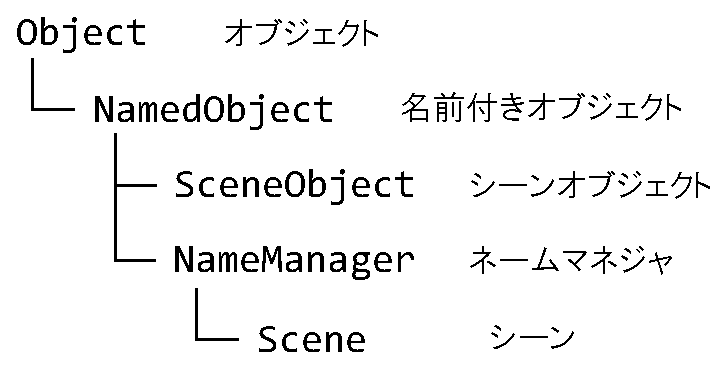
\includegraphics[width=.5\hsize]{fig/utclass.eps}
\end{center}
\caption{Object class hierarchy}
\label{fig_utclass}
\end{figure}

\index{Object}
�قƂ�ǂ��ׂĂ�Springhead�I�u�W�F�N�g��\texttt{Object}�N���X����h�����܂��D
�I�u�W�F�N�g�͕����̎q�I�u�W�F�N�g�����‚��Ƃ��ł��܂��D
Springhead�̃f�[�^�\���̓I�u�W�F�N�g�������c���[�\���ɂ���ďo���オ���Ă��܂��D
Foundation���W���[���ɂ�����\texttt{Object}����̃N���X�K�w��Fig.\,\ref{fig_utclass}�Ɏ����܂��D

�܂�\texttt{Object}�N���X�̎q�I�u�W�F�N�g�̍쐬�E�Ǘ��Ɋ֌W����֐����Љ�܂��D

\noindent
\begin{tabular}{p{1.0\hsize}}
\\
\texttt{ObjectIf}										\\ \midrule
\texttt{size\_t NChildObject()}							\\
�q�I�u�W�F�N�g�̐����擾����D							\\
														\\
\texttt{ObjectIf* GetChildObject(size\_t pos)}			\\
\texttt{pos}�Ԗڂ̎q�I�u�W�F�N�g���擾����D			\\
														\\
\texttt{bool AddChildObject(ObjectIf* o)}				\\
�I�u�W�F�N�g\texttt{o}���q�I�u�W�F�N�g�Ƃ��Ēlj�����D
�������lj����ꂽ��\texttt{true}�C����ȊO��\texttt{false}��Ԃ��D\\
														\\
\texttt{bool DelChildObject(ObjectIf* o)}				\\
�I�u�W�F�N�g\texttt{o}���q�I�u�W�F�N�g����폜����D
�������폜���ꂽ��\texttt{true}�C����ȊO��\texttt{false}��Ԃ��D\\
														\\
\texttt{void Clear();}									\\
�N���A����D												\\
\\
\end{tabular}

�����̊֐��͔h���N���X�ɂ���Ď�������܂��̂ŁC�lj��ł���q�I�u�W�F�N�g�̎�ނ␔�Ȃǂ̓N���X���ƂɈقȂ�܂��D
�܂��CSpringhead�𕁒ʂɎg�p����͈͓��ł̓��[�U�������̊֐��𒼐ڌĂяo����ʂ͂Ȃ��ł��傤�D

�X�g���[���o�͂̂��߂Ɉȉ��̋@�\������܂��D

\noindent
\begin{tabular}{p{1.0\hsize}}
\\
\texttt{ObjectIf}										\\ \midrule
\texttt{void Print(std::ostream\& os) const}			\\
�I�u�W�F�N�g�̓��e���X�g���[��\texttt{os}�ɏo�͂���D	\\
\\
\end{tabular}
\texttt{Print}�́C��{�I�ɂ͂��̃I�u�W�F�N�g�̖��O���o�͂��C�q�I�u�W�F�N�g��\texttt{Print}���ċA�I�ɌĂяo���܂��D
�������h���N���X�ɂ����\texttt{Print}�ŏo�͂������e���J�X�^�}�C�Y����Ă���ꍇ�͂��̌���ł͂���܂���D

\texttt{NamedObject}�͖��O�t���I�u�W�F�N�g�ł��D
\texttt{NamedObject}�̔h���N���X�ɂ͖��O�𕶎���ŗ^���邱�Ƃ��ł��C���O����I�u�W�F�N�g���������邱�Ƃ��ł��܂��D
���O�t���I�u�W�F�N�g�ɂ́C���ڂ̐e�I�u�W�F�N�g�ȊO�ɁC���O���Ǘ����邽�߂̃l�[���}�l�W�����Ή����܂��D

\noindent
\begin{tabular}{p{1.0\hsize}}
\\
\texttt{NamedObjectIf}									\\ \midrule
\texttt{const char* GetName()}			\\
���O���擾����D						\\
\\
\texttt{void SetName(const char* n)}	\\
���O��ݒ肷��D						\\
\\
\texttt{NameManagerIf* GetNameManager()}	\\
�l�[���}�l�W�����擾����D					\\
\\
\end{tabular}

���O�t���I�u�W�F�N�g����͂���ɃV�[���I�u�W�F�N�g���h�����܂��D
�V�[���I�u�W�F�N�g����͎��Ӄ��W���[���̃I�u�W�F�N�g(\texttt{PHSolid}, \texttt{GRVisual}�Ȃ�)���h�����܂��D

\noindent
\begin{tabular}{p{1.0\hsize}}
\\
\texttt{SceneObjectIf}					\\ \midrule
\texttt{SceneIf* GetScene()}			\\
���g����������V�[�����擾����D		\\
\\
\end{tabular}

\section{�l�[���}�l�W���ƃV�[��}

\index{NameManager}
�l�[���}�l�W���͖��O�t���I�u�W�F�N�g�̃R���e�i�Ƃ��ē����C�����̖��O���Ǘ����܂��D
�܂��C�l�[���}�l�W���͂��ꎩ�g���O�t���I�u�W�F�N�g�ł��D

\noindent
\begin{tabular}{p{1.0\hsize}}
\\
\texttt{NameManagerIf}									\\ \midrule
\texttt{NamedObjectIf* FindObject(UTString name)}		\\
���O��\texttt{name}�̃I�u�W�F�N�g���������C���‚���΂��̃I�u�W�F�N�g��Ԃ��D
���‚���Ȃ����\texttt{NULL}��Ԃ��D					\\
\\
\end{tabular}


\index{Scene}
�V�[���̓V�[���I�u�W�F�N�g�̃R���e�i�ł��D
�V�[���̊�{�N���X��\texttt{Scene}�ŁC��������e���W���[���̃V�[��(\texttt{PHScene}, \texttt{GRScene}, \texttt{FWScene}�Ȃ�)���h�����܂��D
\texttt{Scene}�N���X�͓��ɋ@�\��񋟂��܂���D


\section{�^�C�}}
\label{sec_uttimer}

\index{UTTimer}
\index{������@�^�C�}}
�^�C�}�@�\��Foundation�Œ񋟂���܂��D
�^�C�}�N���X��\texttt{UTTimer}�ł��D
�^�C�}���쐬����ɂ�
\begin{sourcecode}
UTTimerIf* timer = UTTimerIf::Create();
\end{sourcecode}
�Ƃ��܂��D\texttt{UTTimer}�ɂ͈ȉ���API������܂��D
\begin{center}
\begin{tabular}{ll}
\texttt{[Get|Set]Resolution}		& ����\�̎擾�Ɛݒ�	\\
\texttt{[Get|Set]Interval}			& �����̎擾�Ɛݒ�		\\
\texttt{[Get|Set]Mode}				& ���[�h�̎擾�Ɛݒ�	\\
\texttt{[Get|Set]Callback}			& �R�[���o�b�N�֐��̎擾�Ɛݒ� \\
\texttt{IsStarted}					& �����Ă��邩�ǂ���	\\
\texttt{IsRunning}					& �R�[���o�b�N�Ăяo���� \\
\texttt{Start}						& �n��	\\
\texttt{Stop}						& ��~	\\
\texttt{Call}						& �R�[���o�b�N�Ăяo��
\end{tabular}
\end{center}
\texttt{SetMode}�Ŏw��ł��郂�[�h�ɂ͈ȉ�������܂��D
\begin{center}
\begin{tabular}{ll}
\texttt{MULTIEDIA}		& �}���`���f�B�A�^�C�}			\\
\texttt{THREAD}		& �Ɨ��X���b�h					\\
\texttt{FRAMEWORK}		& Framework���񋟂���^�C�}		\\
\texttt{IDLE}			& Framework���񋟂���A�C�h���R�[���o�b�N
\end{tabular}
\end{center}
�}���`���f�B�A�^�C�}��Windows���񋟂��鍂�@�\�^�C�}�ł��D
�Ɨ��X���b�h���[�h�ł́C�^�C�}�p�̃X���b�h�����s����\texttt{Sleep}�֐��ɂ����������䂳��܂��D
\texttt{FRAMEWORK}��\texttt{IDLE}���[�h�𗘗p����ɂ�\texttt{FWApp}��\texttt{CreateTimer}�֐���p����K�v������܂��D
��{�I��\texttt{FRAMEWORK}���[�h�ł�GLUT�̃^�C�}�R�[���o�b�N���g���C
\texttt{IDLE}���[�h�ł�GLUT�̃A�C�h���R�[���o�b�N���g���܂��D

Framework���W���[����\texttt{FWApp}�𗘗p����ꍇ�́C\texttt{FWApp}��\texttt{CreateTimer}�֐��𗘗p��������֗��ł��傤�D


\section{��Ԃ̕ۑ��E�Č�}
�V�~�����[�V�������s���ƁA�V�[�����\������I�u�W�F�N�g�̏�Ԃ��ω�����B
���鎞���ł̏�Ԃ�ۑ����Ă����A�Č����邱�Ƃ��ł���ƁA���X�e�b�v�O�ɖ߂�����A����X�e�b�v�̃V�~�����[�V�������A�͂��������ꍇ�Ɖ����Ȃ��ꍇ�Ŕ�ׂ���Ƃ�������Ƃ��ł���B
Springhead�ł́A\texttt{ObjectStatesIf}��p���邱�ƂŁA�ȉ��̂悤�ɃV�[���S�̂̏�Ԃ��܂Ƃ߂ă�������ɕۑ��A�Č����邱�Ƃ��ł���B

\begin{sourcecode}
	PHSceneIf* phScene;
	�ȗ��FphScene�i�����V�~�����[�V�����̃V�[���j�̍\�z
	UTRef<ObjectStatesIf> states;
	states = ObjectStatesIf::Create();	// ObjectStates�I�u�W�F�N�g�̍쐬
	states->AllocateState(phScene);		// �ۑ��p�̃������m��
	states->SaveState(phScene);			// ��Ԃ̕ۑ�
	phScene->Step();					// ���̃V�~�����[�V������i�߂�
	�ȗ��F�����x�̎擾�Ȃ�
	states->LoadState(phScene);			// ��Ԃ̍Č�
	states->ReleaseState();				// �������̊J��
	�ȗ��F�͂�������Ȃǂ̏���
	phScene->Step();					// �{�Ԃ̃V�~�����[�V������i�߂�
\end{sourcecode}

\subsection{�ۑ��E�Č��̃^�C�~���O}
Springhead�̃V�[��(PHScene��CRScene)�́A�����̃G���W��(PHEngine��CREngine�̔h���N���X)���Ăяo�����ƂŁA�V�~�����[�V������i�߂�B
�V�[���́A�G���W���̌Ăяo�����ȊO�̃^�C�~���O�ł���΂��‚ł���Ԃ�ۑ��E�Č����邱�Ƃ��ł���B

\subsection{�V�[���\���ύX�̐���}
��ԕۑ��p�̃������́A�V�[���̍\���Ɉˑ����Ă���B\texttt{AllocateState(), SaveState(), LoadState()}�����łȂ��A\texttt{ObjectStatesIf::ReleaseState()}���ˑ�����̂ŁA\texttt{ObjectIf::AddChildObject()}�Ȃǂ�API�ɂ���ăV�[���̍\����ω������Ă��܂��ƁA�ۑ��E�Č������łȂ��������̊J�����ł��Ȃ��Ȃ�B�ύX�O�ɊJ�����邩�A�V�[���\����߂��Ă���J������K�v������B


\chapter{Collision}
\label{chap_collision}
\section{�T�v}

\index{Collision}
Collision���W���[���͕����v�Z�̊�b�ƂȂ�Փ˔���@�\��񋟂��܂��D
������Collision���W���[����Physics���W���[���̃T�u���W���[���ƂȂ��Ă���C���҂͖��ڂɈˑ����Ă��܂��D
���[�U�͎�Ƃ��č��̂ɏՓ˔���p�`������蓖�Ă�ۂ�Collision���W���[���̋@�\�𗘗p���邱�ƂɂȂ�܂��D

\begin{figure}[t]
\begin{center}
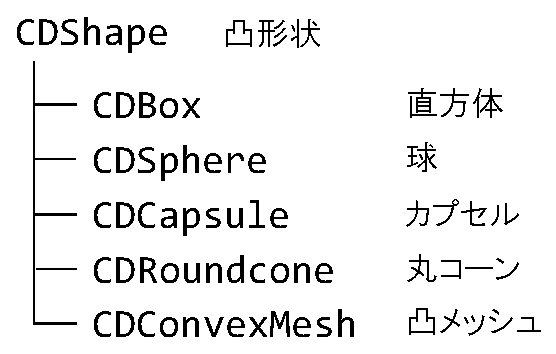
\includegraphics[width=.4\hsize]{fig/cdclass.eps}
\end{center}
\caption{Class hierarchy of Collision module}
\label{fig_cdclass}
\end{figure}

\index{CDShape}
Collision���W���[���̃N���X�K�w��Fig.\,\ref{fig_cdclass}�Ɏ����܂��D
�Փ˔���`��͂��ׂ�\url{CDShape}����h�����܂��D
�A���S���Y���̐�����C�`��͂��ׂēʌ`��łȂ���΂Ȃ�܂���D

\section{�`��̍쐬}

�Փ˔���`��͎��̎菇�ō쐬�E�o�^���܂��D
\begin{enumerate}
\item �`����쐬����
\item ���̂֌`���lj�����
\item �`��̈ʒu��ݒ肷��
\end{enumerate}
�ȉ��ɏ���ǂ��Đ������܂��D

�܂��`����쐬����ɂ͎��̂悤�ɂ��܂��D
\begin{sourcecode}
// given PHSdkIf* phSdk

CDBoxDesc desc;
desc.boxsize = Vec3d(1.0, 1.0, 1.0);

CDBoxIf* box = phSdk->CreateShape(desc)->Cast();
\end{sourcecode}
�Փ˔���`��̃I�u�W�F�N�g��Physics���W���[�����Ǘ����܂��D
���̂��߁C�`����쐬����ɂ�\url{PHSdk}�N���X��\url{CreateShape}�֐����g���܂��D
\url{PHSdk}�ɂ‚��Ă�\ref{chap_physics}�͂��Q�Ƃ��Ă��������D
�`����쐬����ɂ́C�܂���ނɉ������f�B�X�N���v�^���쐬���C���@�Ȃǂ̃p�����[�^��ݒ肵�܂��D
���̗�ł͒����̃N���X\url{CDBox}�̃f�B�X�N���v�^���쐬���Ĉ�ӂ�$1.0$�̗����̂��쐬���܂��D
�f�B�X�N���v�^���w�肵��\url{CreateShape}���Ăяo���ƁC�Ή������ނ̌`�󂪍쐬����C
���̃C���^�t�F�[�X���Ԃ���܂��D
�������߂�l�͌`��̊��N���X�ł���\url{CDShape}�̃C���^�t�F�[�X�ł��̂ŁC�h���N���X�i�����ł�\url{CDBox}�j�̃C���^�t�F�[�X�𓾂�ɂ�
��̂悤��\url{Cast}�֐��œ��I�L���X�g����K�v������܂��D

�`����쐬������C���ɂ��̌`���^���������̂ɓo�^���܂��D
\begin{sourcecode}
// given PHSolidIf* solid

solid->AddShape(box);         // first box
\end{sourcecode}
���̃N���X\url{PHSolid}�ɂ‚��Ă�\ref{chap_physics}�͂��Q�Ƃ��Ă��������D
�����ŏd�v�Ȃ��Ƃ́C��x�쐬�����`���1�‚̍��̂ɂ����‚ł��o�^�ł��C�܂��قȂ镡���̍��̂ɂ��o�^�ł���Ƃ������Ƃł��D
�‚܂�C�����`��𕡐��̍��̊Ԃŋ��L���邱�ƂŁC�`��̍쐬�R�X�g�⃁���������}���邱�Ƃ��ł��܂��D

\url{AddShape}�֐��œo�^��������̌`��́C���̂̃��[�J�����W�n�̌��_�Ɉʒu���Ă��܂��D
�����ύX�������ꍇ��\url{SetShapePose}�֐����g���܂��D
\begin{sourcecode}
solid->AddShape(box);         // second box
solid->AddShape(box);         // third box 

// move first shape 1.0 in x-direction
solid->SetShapePose(0, Posed(Vec3d(1.0, 0.0, 0.0), Quaterniond());

// rotate second shape 30 degrees along y-axis
solid->SetShapePose(1, Posed(Vec3d(),
                    Quaterniond::Rot(Rad(30.0), 'y')));
\end{sourcecode}
\url{SetShapePose}�̑�1�����͑��삷��`��̔ԍ��ł��D�ŏ���\url{AddShape}�����`��̔ԍ���$0$�ŁC\url{AddShape}���邽�т�$1$�������܂��D
�`��̈ʒu������͍��̂̃��[�J�����W�n�Ŏw�肵�܂��D
�܂��C�`��̈ʒu�E�������擾����ɂ�\url{GetShapePose}�֐����g���܂��D

�ȉ��ł�Springhead�ŃT�|�[�g����Ă���`�����ޕʂɉ�����܂��D

\subsection*{������}

\begin{figure}[t]
\begin{center}
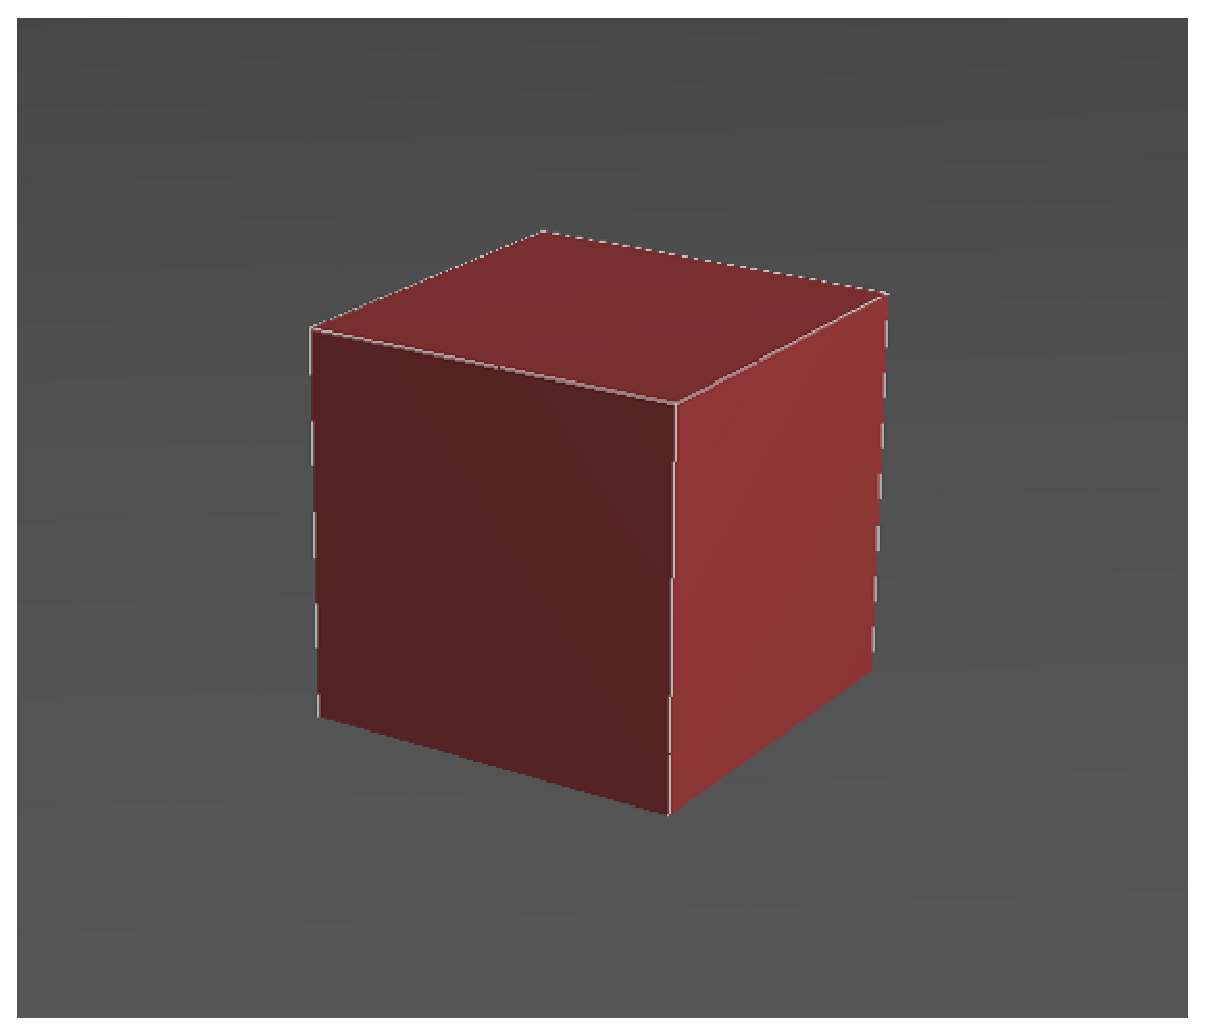
\includegraphics[width=.4\hsize]{fig/cdbox.eps}
\end{center}
\caption{Box geometry}
\label{fig_cdbox}
\end{figure}

\index{CDBox}
\index{���傭�ق�����@������}
������(Fig.\,\ref{fig_cdbox})�̃N���X��\texttt{CDBox}�ł��D

\begin{center}
\begin{tabular}{lll}
\multicolumn{3}{l}{\texttt{CDBoxDesc}}					\\ \midrule
\texttt{Vec3f}	&	\texttt{boxsize}	& �e�ӂ̒��� 	\\
\\
\multicolumn{3}{l}{\texttt{CDBoxIf}}					\\ \midrule
\multicolumn{2}{l}{\texttt{Vec3f GetBoxSize()}}			\\
\multicolumn{2}{l}{\texttt{void SetBoxSize(Vec3f)}}		\\
\end{tabular}
\end{center}


\subsection*{��}

\begin{figure}[t]
\begin{center}
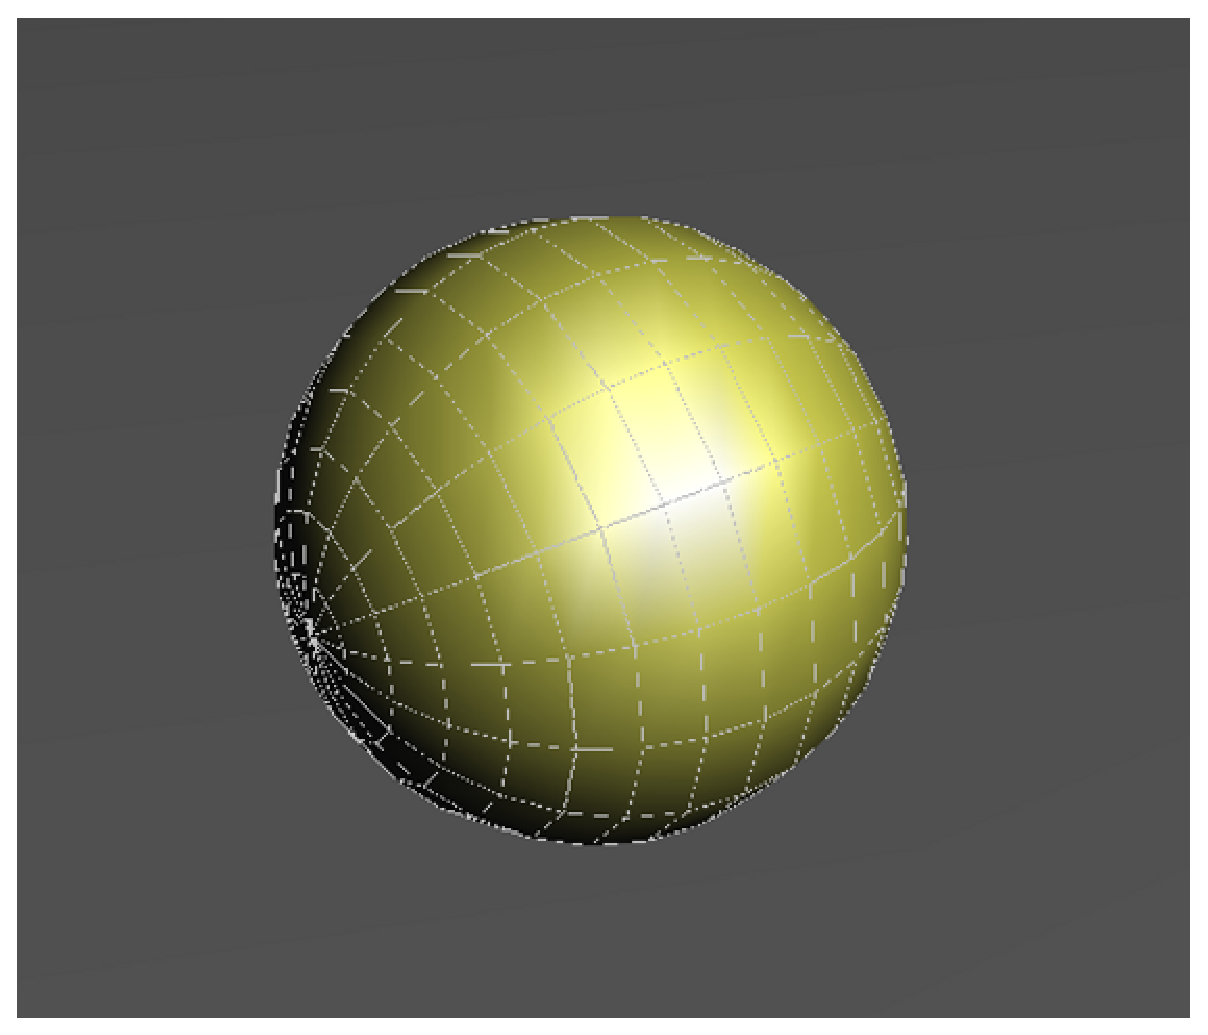
\includegraphics[width=.4\hsize]{fig/cdsphere.eps}
\end{center}
\caption{Sphere geometry}
\label{fig_cdsphere}
\end{figure}

\index{CDSphere}
\index{���イ@��}
��(Fig.\,\ref{fig_cdsphere})�̃N���X��\url{CDSphere}�ł��D

\begin{center}
\begin{tabular}{lll}
\multicolumn{3}{l}{\texttt{CDSphereDesc}}				\\ \midrule
\texttt{float}	&	\texttt{radius}	& ���a 				\\
\\
\multicolumn{3}{l}{\texttt{CDSphereIf}}					\\ \midrule
\multicolumn{2}{l}{\texttt{float GetRadius()}}			\\
\multicolumn{2}{l}{\texttt{void SetRadius(float)}}		\\
\end{tabular}
\end{center}


\subsection*{�J�v�Z��}

\begin{figure}[t]
\begin{center}
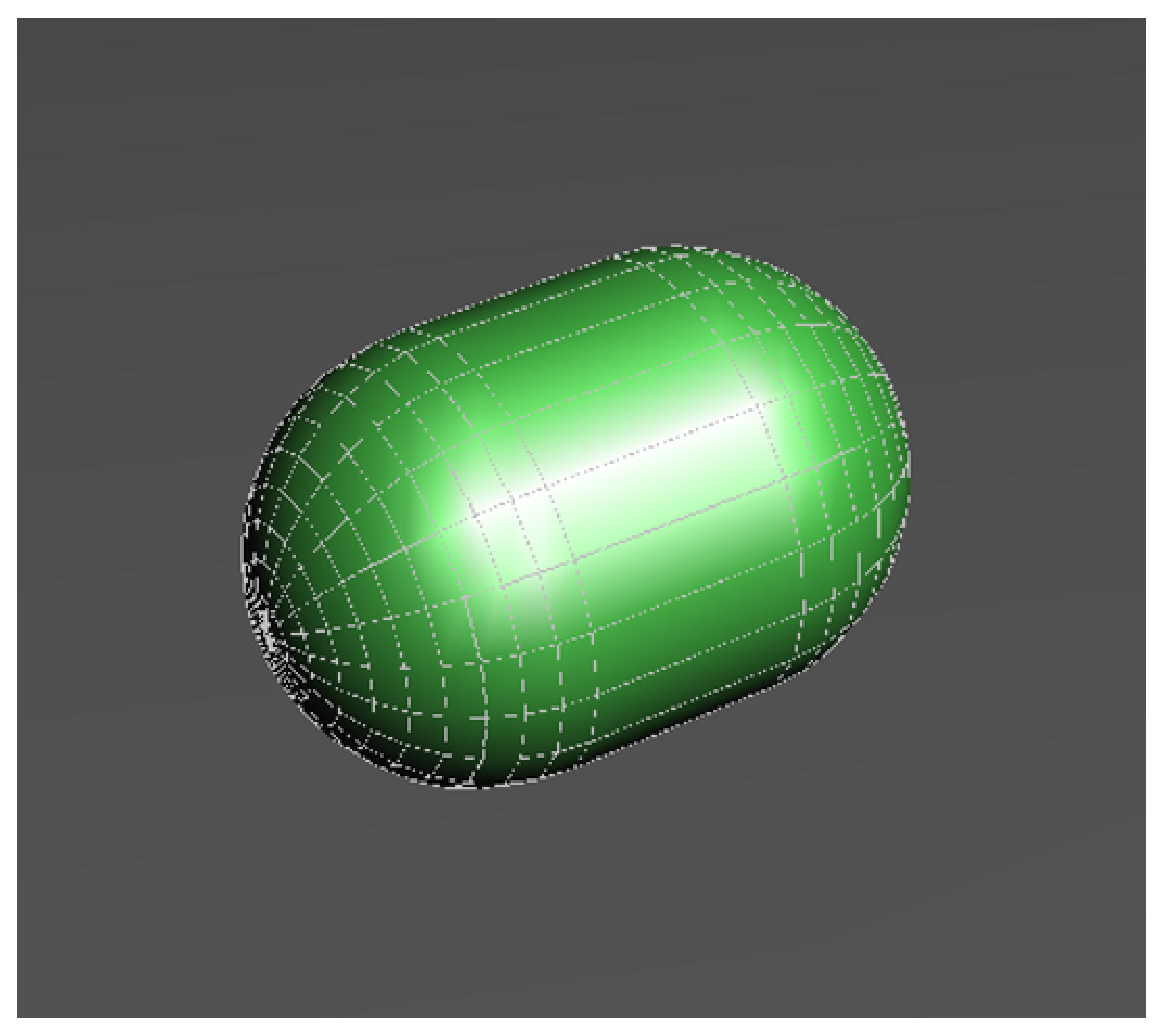
\includegraphics[width=.4\hsize]{fig/cdcapsule.eps}
\end{center}
\caption{Capsule geometry}
\label{fig_cdcapsule}
\end{figure}

\index{CDCapsule}
\index{���Ղ���@�J�v�Z��}
�J�v�Z��(Fig.\,\ref{fig_cdcapsule})�̃N���X��\url{CDCapsule}�ł��D
�J�v�Z���͉~���̗��[�ɔ������‚����`�����Ă��܂��D

\begin{center}
\begin{tabular}{lll}
\multicolumn{3}{l}{\texttt{CDCapsuleDesc}}				\\ \midrule
\texttt{float}	&	\texttt{radius}	& �����̔��a 		\\
\texttt{float}	&	\texttt{length} & �~���̒���		\\
\\
\multicolumn{3}{l}{\texttt{CDCapsuleIf}}				\\ \midrule
\multicolumn{2}{l}{\texttt{float GetRadius()}}			\\
\multicolumn{2}{l}{\texttt{void SetRadius(float)}}		\\
\multicolumn{2}{l}{\texttt{float GetLength()}}			\\
\multicolumn{2}{l}{\texttt{void SetLength(float)}}		\\
\end{tabular}
\end{center}


\subsection*{�ۃR�[��}

\begin{figure}[t]
\begin{center}
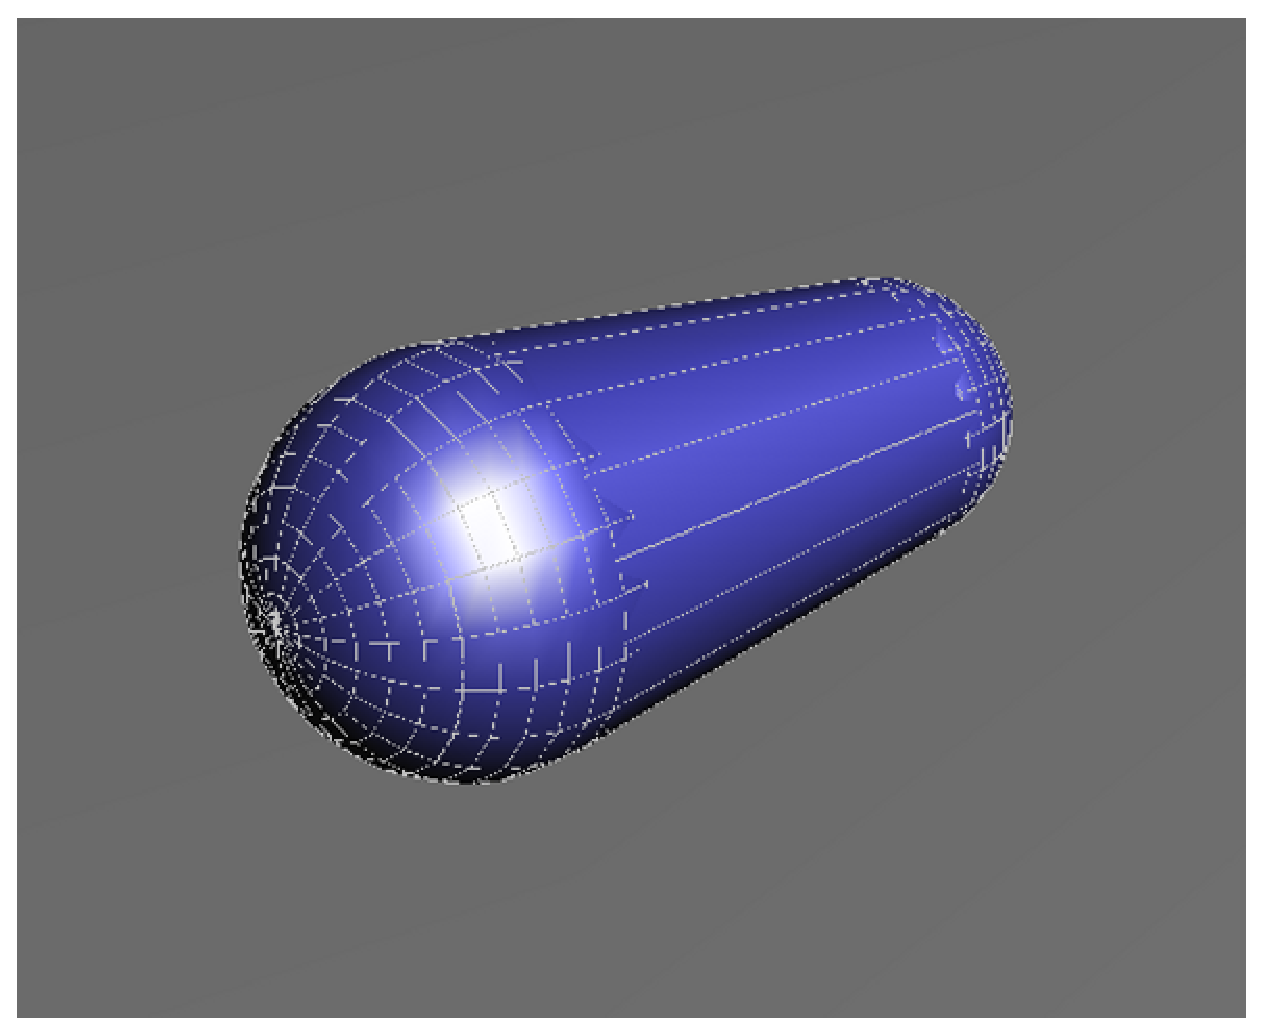
\includegraphics[width=.4\hsize]{fig/cdroundcone.eps}
\end{center}
\caption{Round cone geometry}
\label{fig_cdroundcone}
\end{figure}

\index{CDRoundCone}
\index{�܂邱�[��@�ۃR�[��}
�ۃR�[��(Fig.\,\ref{fig_cdroundcone})�̃N���X��\url{CDRoundCone}�ł��D
�ۃR�[���̓J�v�Z���̗��[�̔��a����Ώ̂ɂȂ������̂ł��D

\begin{center}
\begin{tabular}{lll}
\multicolumn{3}{l}{\texttt{CDRoundConeDesc}}			\\ \midrule
\texttt{Vec2f}	&	\texttt{radius}	& �e�����̔��a		\\
\texttt{float}	&	\texttt{length} & �����Ԃ̋���		\\
\\
\multicolumn{3}{l}{\texttt{CDRoundConeIf}}				\\ \midrule
\multicolumn{2}{l}{\texttt{Vec2f GetRadius()}}			\\
\multicolumn{2}{l}{\texttt{void SetRadius(Vec2f)}}		\\
\multicolumn{2}{l}{\texttt{float GetLength()}}			\\
\multicolumn{2}{l}{\texttt{void SetLength(float)}}		\\
\multicolumn{2}{l}{\texttt{void SetWidth(Vec2f)}}		\\
\end{tabular}
\end{center}

\texttt{SetWidth}�֐��́C�ۃR�[���̑S����ۑ������܂ܔ��a��ύX���܂��D


\subsection*{�ʃ��b�V��}

\begin{figure}[t]
\begin{center}
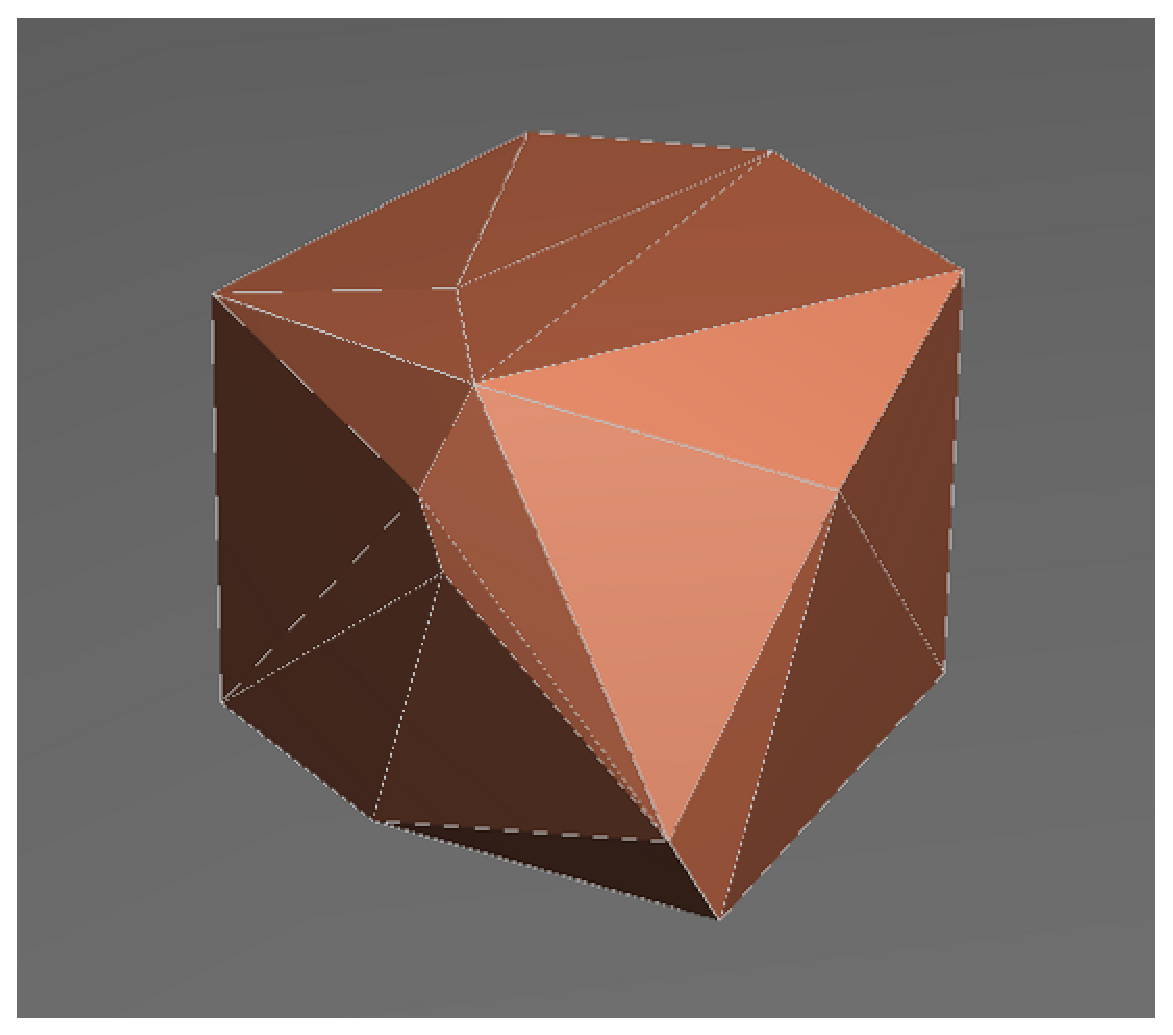
\includegraphics[width=.4\hsize]{fig/cdconvexmesh.eps}
\end{center}
\caption{Convex mesh geometry}
\label{fig_cdconvexmesh}
\end{figure}

\index{CDConvexMesh}
\index{�Ƃ‚߂�����@�ʃ��b�V��}
�ʃ��b�V��(Fig.\,\ref{fig_cdconvexmesh})�̃N���X��\url{CDConvexMesh}�ł��D
�ʃ��b�V���Ƃ͉��݂⌊�������Ȃ����ʑ̂ł��D
���_���W���w�肷�邱�ƂŎ��R�Ȍ`���쐬���邱�Ƃ��ł��܂��D

\begin{center}
\begin{tabular}{lll}
\multicolumn{3}{l}{\texttt{CDConvexMeshDesc}}						\\ \midrule
\texttt{vector<Vec3f>}	&	\texttt{vertices}	& ���_���W�̔z��	\\
\\
\multicolumn{3}{l}{\texttt{CDConvexMeshIf}}					\\ \midrule
\multicolumn{2}{l}{\texttt{Vec3f* GetVertices()}}			& ���_�z��̐擪�A�h���X	\\
\multicolumn{2}{l}{\texttt{int NVertex()}}					& ���_��					\\
\multicolumn{2}{l}{\texttt{CDFaceIf* GetFace(int i)}}		& $i$�Ԗڂ̖�				\\
\multicolumn{2}{l}{\texttt{int NFace()}}					& �ʐ�						\\
\end{tabular}
\end{center}

�ʃ��b�V�����쐬�����ہC\texttt{CDConvexMeshDesc::vertices}�Ɋi�[���ꂽ���_������ŏ��̓ʑ��ʑ́i�ʕ�j���쐬����܂��D
���ʑ̖̂ʂ�\��\texttt{CDFace}�̃C���^�t�F�[�X���ȉ��Ɏ����܂��D

\begin{center}
\begin{tabular}{lll}
\multicolumn{3}{l}{\texttt{CDFaceIf}}						\\ \midrule
\multicolumn{2}{l}{\texttt{int* GetIndices()}}				& ���_�C���f�b�N�X�z��̐擪�A�h���X	\\
\multicolumn{2}{l}{\texttt{int NIndex()}}					& �ʂ̒��_��							\\
\end{tabular}
\end{center}

\texttt{NIndex}�͖ʂ��\�����钸�_�̐���Ԃ��܂��i�ʏ�$3$��$4$�ł��j�D
�ʂ͒��_�z��𒼐ڕۗL�����C�C���f�b�N�X�z��Ƃ��ĊԐړI�ɒ��_���Q�Ƃ��܂��D
���������āC�ʂ̒��_���W�𓾂�ɂ�
\begin{sourcecode}
// given CDConvexMeshIf* mesh
CDFaceIf* face = mesh->GetFace(0);        // get 0-th face
int* idx = face->GetIndices();
Vec3f v = mesh->GetVertices()[idx[0]];    // get 0-th vertex
\end{sourcecode}
�Ƃ��܂��D

\section{�����̎w��}
\label{sec_collision_material}

\index{PHMaterial}
\index{�Ԃ�����@����}
�`��ɂ͖��C�W���⒵�˕Ԃ�W���Ȃǂ̕������w�肷�邱�Ƃ��ł��܂��D
�`��̊�{�N���X�ł���\texttt{CDShape}�̃f�B�X�N���v�^\texttt{CDShapeDesc}��\texttt{PHMaterial}�^�̕ϐ�\texttt{material}�������Ă��܂��D

\begin{center}
\begin{tabular}{lll}
\multicolumn{3}{l}{\texttt{PHMaterial}}							\\ \midrule
\texttt{float}	&	\texttt{density}		& ���x				\\
\texttt{float}	&	\texttt{mu0}			& �Î~���C�W��		\\
\texttt{float}	&	\texttt{mu}				& �����C�W��		\\
\texttt{float}	&	\texttt{e}				& ���˕Ԃ�W��		\\
\texttt{float}	&	\texttt{reflexSpring}	& ���˕Ԃ�o�l�W���i�y�i���e�B�@�j	\\
\texttt{float}	&	\texttt{reflexDamper}	& ���˕Ԃ�_���p�W���i�y�i���e�B�@�j\\
\texttt{float}	&	\texttt{frictionSpring}	& ���C�o�l�W���i�y�i���e�B�@�j	\\
\texttt{float}	&	\texttt{frictionDamper}	& ���C�_���p�W���i�y�i���e�B�@�j\\
\end{tabular}
\end{center}

�`��쐬��ɕ������w�肷��ɂ�\texttt{CDShapeIf}�̊֐����g���܂��D

\begin{center}
\begin{tabular}{lll}
\multicolumn{3}{l}{\texttt{CDShapeIf}}						\\ \midrule
\multicolumn{2}{l}{\texttt{void SetDensity(float)}}				& \\
\multicolumn{2}{l}{\texttt{float GetDensity()}}					& \\
\multicolumn{2}{l}{\texttt{void SetStaticFriction(float)}}		& \\
\multicolumn{2}{l}{\texttt{float GetStaticFriction()}}			& \\
\multicolumn{2}{l}{\texttt{void SetDynamicFriction(float)}}		& \\
\multicolumn{2}{l}{\texttt{float GetDynamicFriction()}}			& \\
\multicolumn{2}{l}{\texttt{void SetElasticity(float)}}			& \\
\multicolumn{2}{l}{\texttt{float GetElasticity()}}				& \\
\multicolumn{2}{l}{\texttt{void SetReflexSpring(float)}}		& \\
\multicolumn{2}{l}{\texttt{float GetReflexSpring()}}			& \\
\multicolumn{2}{l}{\texttt{void SetReflexDamper(float)}}		& \\
\multicolumn{2}{l}{\texttt{float GetReflexDamper()}}			& \\
\multicolumn{2}{l}{\texttt{void SetFrictionSpring(float)}}		& \\
\multicolumn{2}{l}{\texttt{float GetFrictionSpring()}}			& \\
\multicolumn{2}{l}{\texttt{void SetFrictionDamper(float)}}		& \\
\multicolumn{2}{l}{\texttt{float GetFrictionDamper()}}			& \\
\end{tabular}
\end{center}

�����Ɋ�Â����ڐG�͂̋�̓I�Ȍv�Z�@�ɂ‚��Ă͑�\ref{sec_physics_contact}�߂��Q�Ƃ��ĉ������D

\section{�􉽏��̌v�Z}

�`��Ɋւ���􉽏����v�Z����֐����Љ�܂��D

\begin{center}
\begin{tabular}{lll}
\multicolumn{3}{l}{\texttt{CDShapeIf}}							\\ \midrule
\multicolumn{2}{l}{\texttt{float CalcVolume()}}					& �̐ς��v�Z		\\
\multicolumn{2}{l}{\texttt{Vec3f CalcCenterOfMass()}}			& ���ʒ��S���v�Z	\\
\multicolumn{2}{l}{\texttt{Matrix3f CalcMomentOfInertia()}}		& �����s����v�Z	\\
\end{tabular}
\end{center}

\texttt{CalcVolume}�͌`��̑̐ς��v�Z���܂��D�̐ςɖ��x�i\texttt{GetDensity}�Ŏ擾�j���|����Ύ��ʂ������܂��D
\texttt{CalcCenterOfMass}�֐��́C�`��̃��[�J�����W�n�ŕ\���ꂽ���ʒ��S�̍��W���v�Z���܂��D
\texttt{CalcMomentOfInertia}�֐��́C�`��̃��[�J�����W�n�ŕ\���ꂽ���ʒ��S�Ɋւ��銵���s����v�Z���܂��D
�������C���x��$1$�Ƃ����ꍇ�̒l���Ԃ���܂��̂ŁC���ۂ̊����s��𓾂�ɂ͖��x���|����K�v������܂��D



\chapter{Physics}
\label{chap_physics}
\section{�T�v}

\index{Physics}
Physics���W���[���͕����V�~�����[�V�����@�\��񋟂��܂��D
��ɃT�|�[�g����Ă���̂́C�}���`�{�f�B�_�C�i�~�N�X�ƌĂ΂�鍄�̂Ɗ֐߂Ȃǂ̍S������Ȃ铮�͊w�V�~�����[�V�����ł��D
���̂Ƃ���\�t�g�{�f�B�◬�́C�p�[�e�B�N���Ȃǂ̋@�\�̓T�|�[�g����Ă��܂���D

\section{Physics SDK}

\index{PHSdk}
Physics���W���[���̂��ׂẴI�u�W�F�N�g��SDK�N���X\texttt{PHSdk}�ɂ���ĊǗ�����܂��D
\texttt{PHSdk}�N���X�́C�v���O�����̎��s��ʂ��Ă����P�‚̃I�u�W�F�N�g�����݂���V���O���g���N���X�ł��D
\texttt{PHSdk}�I�u�W�F�N�g���쐬����ɂ͈ȉ��̂悤�ɂ��܂��D
\begin{sourcecode}
PHSdkIf* phSdk = PHSdkIf::CreateSdk();
\end{sourcecode}
�ʏ킱�̑���̓v���O�����̏��������Ɉ�x�������s���܂��D
�܂��CFramework���W���[�����g�p����ꍇ�̓��[�U������\texttt{PHSdk}���쐬����K�v�͂���܂���D

\texttt{PHSdk}�̋@�\�̓V�[���ƌ`��̊Ǘ��ł��D
�V�[���Ɋւ���@�\�͎��߂Ő������܂��D
�܂��C�`��Ɋւ���@�\�͈ȉ��̒ʂ�ł��D

\begin{center}
\begin{tabular}{p{.15\hsize}p{.55\hsize}p{.2\hsize}}
\texttt{PHSdkIf} & &															\\ \midrule
\texttt{CDShapeIf*} & \texttt{CreateShape(const CDShapeDesc\&)}	& �`����쐬	\\
\texttt{CDShapeIf*}	& \texttt{GetShape(int)}					& �`����擾	\\
\texttt{int}		& \texttt{NShape()}							& �`��̐�		\\
\end{tabular}
\end{center}

�قȂ�V�[���ԂŌ`������L�ł���悤�ɁC�`��Ǘ��̓V�[���ł͂Ȃ�\texttt{PHSdk}�̋@�\�ɂȂ��Ă��܂��D
�ڂ�����\ref{chap_collision}�͂��Q�Ƃ��Ă��������D

\section{�V�[��}
\label{sec_physics_scene}

\index{PHScene}
�V�[���͕����V�~�����[�V�������s���‹���\���܂��D
�����̃V�[�����쐬�ł��܂����C�V�[�����m�݂͌��ɓƗ����Ă���C���[�U�����ڋ��n�����������Ȃ�����͉e�����y�ڂ��������Ƃ͂���܂���D
�V�[���N���X��\texttt{PHScene}�ŁC\texttt{PHScene}�I�u�W�F�N�g��\texttt{PHSdk}�ɂ��Ǘ�����܂��D

\begin{center}
\begin{tabular}{p{.15\hsize}p{.55\hsize}p{.2\hsize}}
\multicolumn{3}{l}{\texttt{PHSdkIf}}															\\ \midrule
\texttt{PHSceneIf*}	& \texttt{CreateScene(const PHSceneDesc\& desc)}			& �V�[�����쐬		\\
\texttt{int}		& \texttt{NScene()}											& �V�[���̐�		\\
\texttt{PHSceneIf*}	& \texttt{GetScene(int i)}									& �V�[�����擾		\\
\texttt{void}		& \texttt{MergeScene(PHSceneIf* scene0, PHSceneIf* scene1)}	& �V�[���𓝍�		\\
\end{tabular}
\end{center}

�V�[�����쐬����ɂ͈ȉ��̂悤�ɂ��܂��D
\begin{sourcecode}
PHSceneIf* phScene = phSdk->CreateScene();
\end{sourcecode}
�����Ƀf�B�X�N���v�^���w�肷�邱�Ƃ��ł��܂��D
\texttt{MergeScene}�́C\texttt{scene1}���ۗL����I�u�W�F�N�g�����ׂ�\texttt{scene0}�Ɉړ��������\texttt{scene1}���폜���܂��D

�V�[���͍��̂�֐߂Ȃǂ̗l�X�ȍ\���v�f�̊Ǘ����s���ق��C�����V�~�����[�V�����Ɋւ���ݒ���s���@�\��񋟂��܂��D
�e�\���v�f�̍쐬�ɂ‚��Ă͂��ꂼ��̐߂Ő������܂��̂ŁC�ȉ��ł̓V�~�����[�V�����ݒ�@�\�ɂ‚��ďq�ׂ܂��D

\begin{center}
\begin{tabular}{p{.15\hsize}p{.35\hsize}p{.4\hsize}}
\multicolumn{3}{l}{\texttt{PHSceneDesc}}										\\ \midrule
\texttt{double}		&	\texttt{timeStep}	& ���ԃX�e�b�v��					\\
\texttt{unsigned}	&	\texttt{count}		& �V�~�����[�V���������X�e�b�v��	\\
\texttt{Vec3d}		&	\texttt{gravity}	& �d�͉����x						\\
\texttt{double}		&	\texttt{airResistanceRate}	& ��C��R�W��				\\
\texttt{int}		&	\texttt{numIteration}		& LCP�̔�����				\\
\end{tabular}
\end{center}

\begin{center}
\begin{tabular}{p{.15\hsize}p{.55\hsize}p{.2\hsize}}
\multicolumn{3}{l}{\texttt{PHSceneIf}}							  \\ \midrule
\texttt{double}		& \texttt{GetTimeStep()}					& \\
\texttt{void}		& \texttt{SetTimeStep(double)}				& \\
\texttt{unsigned}	& \texttt{GetCount()}						& \\
\texttt{void}		& \texttt{SetCount(unsigned)}				& \\
\texttt{void}		& \texttt{SetGravity(const Vec3d\&)}		& \\
\texttt{Vec3d}		& \texttt{GetGravity()}						& \\
\texttt{void}		& \texttt{SetAirResistanceRate(double)}		& \\
\texttt{double}		& \texttt{GetAirResistanceRate()}			& \\
\texttt{int}		& \texttt{GetNumIteration()}				& \\
\texttt{void}		& \texttt{SetNumIteration()}				& \\
\end{tabular}
\end{center}

\texttt{timeStep}�͈�x�̃V�~�����[�V�����X�e�b�v�Ői�߂鎞�ԕ��ł��D
�������قǃV�~�����[�V�����̐��x�͏オ��܂����C�������ԃV�~�����[�V������i�߂�̂ɂ�����v�Z�R�X�g�͑��債�܂��D

\texttt{count}�̓V�[���쐬��ɃV�~�����[�V���������ݐσX�e�b�v���ł��D
\texttt{count}��\texttt{timeStep}�̐ς��o�ߎ��Ԃ�\���܂��D

\texttt{gravity}�͏d�͉����x�x�N�g���ł��D

\texttt{airResistanceRate}�́C�V�~�����[�V�����̈��萫�����シ�邽�߂ɖ��X�e�b�v�Ɋe���̂̑��x�Ɋ|������W���ł��D
�Ⴆ��\texttt{airRegistanceRate}��$0.95$�ł���΃X�e�b�v���Ƃɑ��x��$95$\%�ɂȂ�܂��D
���̂悤�ɋ����I�Ɍ����������邱�ƂŁC���x���]���Ɉ��萫�𓾂邱�Ƃ��ł��܂��D

\texttt{numIteration}�́C�S���͂��v�Z���邽�߂ɓ����Ŏ��s�����A���S���Y���̔����񐔂ł��D
��ʂɁC�����񐔂Ɋւ��Ďw���֐��I�ɍS���͂̐��x�����サ�C�v�Z�R�X�g�͔��I�ɑ��債�܂��D

\subsection*{�V�~�����[�V�����̎��s}

�V�~�����[�V������$1$�X�e�b�v�i�߂�ɂ�\texttt{Step}�֐����Ăт܂��D

\begin{center}
\begin{tabular}{p{.15\hsize}p{.3\hsize}p{.45\hsize}}
\multicolumn{3}{l}{\texttt{PHSceneIf}}		\\ \midrule
\texttt{void}	& \texttt{Step()}	& �V�~�����[�V������$1$�X�e�b�v�i�߂� \\
\end{tabular}
\end{center}

\texttt{Step}�����s����ƁC�����܂��ɏq�ׂē����Ŏ��̏������s���܂��D
\begin{itemize}
\item �Փ˔���ƐڐG�S���̐���
\item �S���͂̌v�Z
\item ���̂̑��x����шʒu�̍X�V
\end{itemize}

\section{����}

\index{PHSolid}
���͕̂����V�~�����[�V�����̊�{�v�f�ł��D
���̂̃N���X��\texttt{PHSolid}�ł��D
�܂����̂��쐬�E�Ǘ����邽�߂�\texttt{PHScene}�̊֐��������܂��D

\begin{center}
\begin{tabular}{p{.15\hsize}p{.45\hsize}p{.30\hsize}}
\multicolumn{3}{l}{\texttt{PHSceneIf}}									\\ \midrule
\texttt{PHSolidIf*}		& \texttt{CreateSolid(const PHSolidDesc\&)}	& ���̂��쐬���� \\
\texttt{int}			& \texttt{NSolids()}						& ���̂̐� \\
\texttt{PHSolidIf**} 	& \texttt{GetSolids()}						& ���̔z��̐擪�A�h���X \\
\end{tabular}
\end{center}

���̂��쐬����ɂ�
\begin{sourcecode}
PHSolidIf* solid = phScene->CreateSolid();
\end{sourcecode}
�Ƃ��܂��D�f�B�X�N���v�^���w�肵�č쐬���邱�Ƃ��ł��܂��D
�܂��C\texttt{GetSolids}�͍쐬�������̂��i�[���������z��̐擪�A�h���X��Ԃ��܂��D
���������āC�Ⴆ��$0$�Ԗڂ̍��̂��擾����ɂ�
\begin{sourcecode}
PHSolidIf* solid = phScene->GetSolids()[0];      // get 0-th solid
\end{sourcecode}
�Ƃ��܂��D

�‚��ɍ��̎��g�̋@�\��������܂��D

\subsection*{����}

\begin{center}
\begin{tabular}{p{.15\hsize}p{.45\hsize}p{.30\hsize}}
\multicolumn{3}{l}{\texttt{PHSolidDesc}}							\\ \midrule
\texttt{double}		&	\texttt{mass}		& ����					\\
\texttt{Matrix3d}	&	\texttt{inertia}	& �����s��				\\
\texttt{Vec3d}		&	\texttt{center}		& ���ʒ��S				\\
\texttt{bool}		&	\texttt{dynamical}	& �����@���ɂ���������	\\
\end{tabular}
\end{center}

\begin{center}
\begin{tabular}{p{.15\hsize}p{.45\hsize}p{.30\hsize}}
\multicolumn{3}{l}{\texttt{PHSolidIf}}								\\ \midrule
\texttt{double}		& \texttt{GetMass()}						& \\
\texttt{double} 	& \texttt{GetMassInv()}						& \\
\texttt{void} 		& \texttt{SetMass(double)}					& \\
\texttt{Vec3d} 		& \texttt{GetCenterOfMass()}				& \\
\texttt{void} 		& \texttt{SetCenterOfMass(const Vec3d\&)}	& \\
\texttt{Matrix3d} 	& \texttt{GetInertia()}						& \\
\texttt{Matrix3d} 	& \texttt{GetInertiaInv()}					& \\
\texttt{void} 		& \texttt{SetInertia(const Matrix3d\&)}		& \\
\texttt{void} 		& \texttt{CompInertia()}					& \\
\texttt{void} 		& \texttt{SetDynamical(bool)}				& \\
\texttt{bool} 		& \texttt{IsDynamical()}					& \\
\end{tabular}
\end{center}

\texttt{GetMassInv}��\texttt{GetInertiaInv}�͂��ꂼ�ꎿ�ʂ̋t���Ɗ����s��̋t�s���Ԃ��܂��D
\texttt{CompInertia}�́C���̍��̂����Œ`��Ƃ����̖��x�����Ƃɍ��̂̎��ʁC���ʒ��S�Ɗ����s����v�Z���C�ݒ肵�܂��D
\texttt{dynamical}�́C���̍��̂������@���ɏ]�����ǂ������w�肷��t���O�ł��D
����\texttt{dynamical}��\texttt{true}�̏ꍇ�C���̍��̂ɉ����͂��v�Z����C
�j���[�g���̉^���@���ɂ��������č��̂̑��x���ω����܂��D
����C\texttt{dynamical}��\texttt{false}�̏ꍇ�͊O�͂ɂ��e�����󂯂��C�ݒ肳�ꂽ���x�œ����^�����܂��D
����͂��傤�ǁ��̎��ʂ����ꍇ�Ɠ����ł��D


\subsection*{���}

\begin{center}
\begin{tabular}{p{.15\hsize}p{.45\hsize}p{.30\hsize}}
\multicolumn{3}{l}{\texttt{PHSolidDesc}}							\\ \midrule
\texttt{Vec3d}	&	\texttt{velocity}		& ���x					\\
\texttt{Vec3d}	&	\texttt{angVelocity}	& �p���x				\\
\texttt{Posed}	&	\texttt{pose}			& �ʒu�ƌ���			\\
\end{tabular}
\end{center}

\begin{center}
\begin{tabular}{p{.2\hsize}p{.5\hsize}p{.20\hsize}}
\multicolumn{3}{l}{\texttt{PHSolidIf}}									\\ \midrule
\texttt{Vec3d}			& \texttt{GetVelocity()}						& \\
\texttt{void} 			& \texttt{SetVelocity(const Vec3d\&)}			& \\
\texttt{Vec3d} 			& \texttt{GetAngularVelocity()}					& \\
\texttt{void} 			& \texttt{SetAngularVelocity(const Vec3d\&)}	& \\
\texttt{Posed} 			& \texttt{GetPose()}							& \\
\texttt{void} 			& \texttt{SetPose(const Posed\&)}				& \\
\texttt{Vec3d} 			& \texttt{GetFramePosition()}					& \\
\texttt{void} 			& \texttt{SetFramePosition(const Vec3d\&)}		& \\
\texttt{Vec3d} 			& \texttt{GetCenterPosition()}					& \\
\texttt{void} 			& \texttt{SetCenterPosition(const Vec3d\&)}		& \\
\texttt{Quaterniond} 	& \texttt{GetOrientation()}						& \\
\texttt{void} 			& \texttt{SetOrientation(const Quaterniond\&)}	& \\
\end{tabular}
\end{center}

\texttt{velocity}, \texttt{angVelocity}, \texttt{pose}�͂��ꂼ��O���[�o�����W�n�Ɋւ��鍄�̂̑��x�C�p���x�C�ʒu����ь�����\���܂��D
\texttt{[Get|Set]FramePosition}�̓O���[�o�����W�n�Ɋւ��鍄�̂̈ʒu���擾/�ݒ肵�܂��D
����ɑ΂���\texttt{[Get|Set]CenterPosition}�͍��̂̎��ʒ��S�̈ʒu���擾/�ݒ肵�܂��D
�ΐS���Ă��鍄�̂̓��[�J�����W���_�Ǝ��ʒ��S����v���Ȃ����Ƃɒ��ӂ��Ă��������D
\texttt{[Get|Set]Orientation}�̓O���[�o�����W�n�Ɋւ��鍄�̂̌������擾/�ݒ肵�܂��D


\subsection*{�͂̈���Ǝ擾}

���̂ɉ����͂ɂ�
\begin{itemize}
\item ���[�U���ݒ肷��O��
\item �d��
\item �֐߂�ڐG��������S����
\end{itemize}
��$3$��ނ�����C���ꂼ��ɂ‚��ĕ��i�͂ƃg���N������܂��D
�����ŁC�d�͂͏d�͉����x�ƍ��̂̎��ʂ�茈�܂�C�S���͍͂S�������𖞂����悤�ɓ����Ŏ����I�Ɍv�Z����܂��D
�ȉ��ł̓��[�U�����̂ɉ�����O�͂�ݒ�E�擾������@�������܂��D

\begin{center}
\begin{tabular}{p{.2\hsize}p{.5\hsize}p{.20\hsize}}
\multicolumn{3}{l}{\texttt{PHSolidIf}}								\\ \midrule
\texttt{void} 	& \texttt{AddForce(Vec3d)}					& \\
\texttt{void} 	& \texttt{AddTorque(Vec3d)}					& \\
\texttt{void} 	& \texttt{AddForce(Vec3d, Vec3d)}			& \\
\texttt{Vec3d} 	& \texttt{GetForce()}						& \\
\texttt{Vec3d} 	& \texttt{GetTorque()}						& \\
\end{tabular}
\end{center}

���i�͂�������ɂ�\texttt{AddForce}���g���܂��D
\begin{sourcecode}
solid->AddForce(Vec3d(0.0, -1.0, 0.0));
\end{sourcecode}
�Ƃ���ƍ��̂̎��ʒ��S�ɕ��i��$(0, -1, 0)$�������܂��D�������͂̓O���[�o�����W�n�ŕ\������܂��D
���
\begin{sourcecode}
solid->AddTorque(Vec3d(1.0, 0.0, 0.0));
\end{sourcecode}
�Ƃ���ƍ��̂̎��ʒ��S�Ɋւ��ă��[�����g$(1, 0, 0)$�������܂��D
��p�_��C�ӂɎw�肷��ɂ�
\begin{sourcecode}
solid->AddForce(Vec3d(0.0, -1.0, 0.0), Vec3d(0.0, 0.0, 1.0));
\end{sourcecode}
�Ƃ��܂��D���̏ꍇ�͕��i��$(0, -1, 0)$����p�_$(0, 0, 1)$�ɉ����܂��D
�����ō�p�_�̈ʒu�͍��̂̃��[�J�����W�ł͂Ȃ��O���[�o�����W�ŕ\������邱�Ƃɒ��ӂ��Ă��������D
\texttt{AddForce}��\texttt{AddTorque}�͕�����ĂԂƁC���ꂼ��Ŏw�肵���O�͂̍��͂��ŏI�I�ɍ��̂ɉ����O�͂ƂȂ�܂��D

�O�͂��擾����ɂ�\texttt{GetForce}�C\texttt{GetTorque}���g���܂��D
�������C�����̊֐��Ŏ擾�ł���̂͒��O�̃V�~�����[�V�����X�e�b�v�ō��̂ɍ�p�����O�͂ł��D
���������Ē��O�̃V�~�����[�V�����X�e�b�v���\texttt{AddForce}�����͎͂擾�ł��܂���D
%�V�~�����[�V�����̎��s�Ɨ͂̈���C�擾�Ɋւ���t���[��Fig.\,\ref{fig_addforce}�Ɏ����܂��D


\section{�֐�}

\begin{figure}[t]
\begin{center}
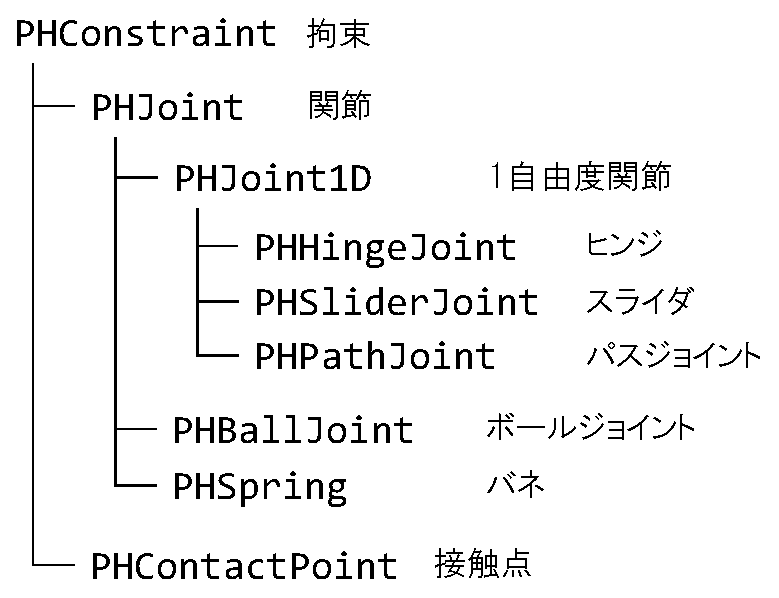
\includegraphics[width=.5\hsize]{fig/phconstraint.eps}
\end{center}
\caption{Constraint class hierarchy}
\label{fig_phconstraint}
\end{figure}

\index{PHConstraint}
\index{PHJoint}
�S���Ƃ͍��̂ƍ��̂̊Ԃɍ�p���Ă��̑��ΓI�^���ɐ����������v�f�ł��D
�S���̃N���X�K�w��Fig.\,\ref{fig_phconstraint}�Ɏ����܂��D
�܂��S���͊֐߂ƐڐG�ɕ�����܂��D�֐߂̓��[�U���쐬���܂����C�ڐG�͏Փ˔��茋�ʂɂ��ƂÂ��Ď����I�ɐ����E�폜����܂��D
�֐߂͂���ɂ����‚��̎�ނɕ������܂��D

�ׂ��Ȑ����͌�񂵂ɂ��āC�܂��͊֐߂̍쐬���@���猩�Ă����܂��D

\subsection*{�֐߂̍쐬}

�ȉ��ł͂����Ƃ��g�p�p�x�̍����q���W�̍쐬���ɂƂ��Ċ֐߂̍쐬���@��������܂��D
�q���W���쐬����ɂ͎��̂悤�ɂ��܂��D
\begin{sourcecode}
PHSolidIf* solid0 = phScene->GetSolids()[0];
PHSolidIf* solid1 = phScene->GetSolids()[1];

PHHingeJointDesc desc;
desc.poseSocket.Pos() = Vec3d( 1.0, 0.0, 0.0);
desc.posePlug.Pos()   = Vec3d(-1.0, 0.0, 0.0);
PHHingeJointIf* joint
    = phScene->CreateJoint(solid0, solid1, desc)->Cast();
\end{sourcecode}
�쐬�������֐߂̎�ނɉ������f�B�X�N���v�^���쐬���C�����\texttt{PHScene}��\texttt{CreateJoint}�֐��ɓn���Ċ֐߂��쐬���܂��D
���̂Ƃ��C�f�B�X�N���v�^�ƂƂ��ɘA�����������̂̃C���^�t�F�[�X���n���܂��D
\texttt{CreateJoint}��\texttt{PHJointIf*}��Ԃ��܂��̂ŁC�쐬�����֐߂̃C���^�t�F�[�X�𓾂�ɂ�\texttt{Cast}�œ��I�L���X�g���܂��D

�֐߂Ɋւ���\texttt{PHScene}�̊֐����ȉ��Ɏ����܂��D

\begin{center}
\begin{tabular}{p{.15\hsize}p{.75\hsize}p{.0\hsize}}
\multicolumn{3}{l}{\texttt{PHSceneIf}}													\\ \midrule
\texttt{PHJointIf*}	& \texttt{CreateJoint(PHSolidIf*, PHSolidIf*, const PHJointDesc\&)}	& \\
\texttt{int}		& \texttt{NJoint()}													& \\
\texttt{PHJointIf*}	& \texttt{GetJoint(int i)}											& \\
\end{tabular}
\end{center}

\texttt{NJoint}�̓V�[�����̊֐߂̌���Ԃ��܂��D\texttt{GetJoint}��\texttt{i}�Ԗڂ̊֐߂��擾���܂��D


\subsection*{�\�P�b�g�ƃv���O}

\index{��������@�\�P�b�g}
\index{�Ղ炮@�v���O}
\begin{figure}[t]
\begin{center}
\begin{tabular}{c}
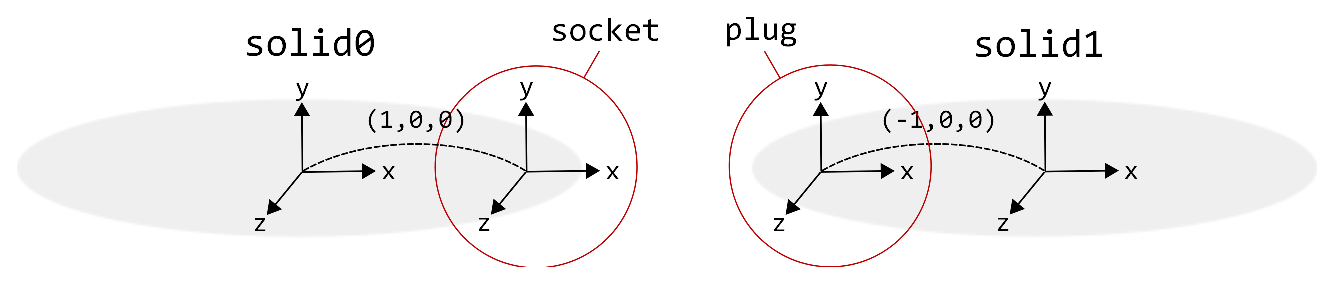
\includegraphics[clip, width=.5\hsize]{fig/socket_plug1.eps} \\
(a) before connection \\
\\
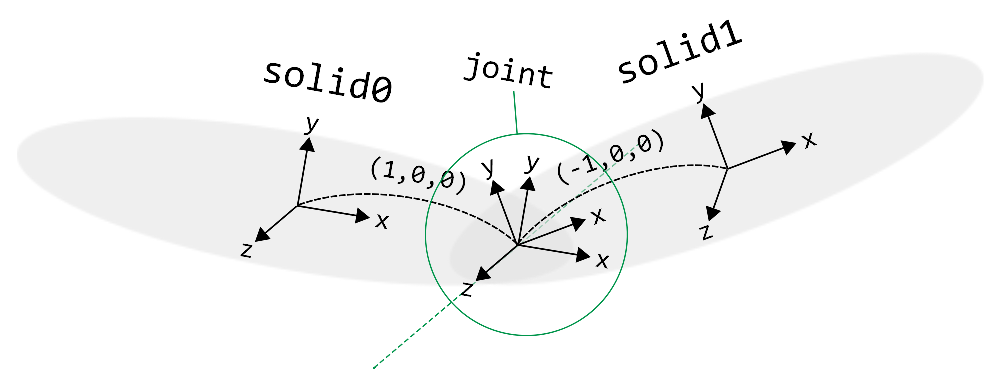
\includegraphics[clip, width=.5\hsize]{fig/socket_plug2.eps} \\
(b) after connection \\
\end{tabular}
\end{center}
\caption{Socket and plug}
\label{fig_socket_plug}
\end{figure}


���āC��̗�Ńf�B�X�N���v�^�ɒl��ݒ肵�Ă���ӏ��ɒ��ڂ��Ă��������D���̕����Ŋ֐߂̎��t���ʒu���w�肵�Ă��܂��D
Springhead�ł́C�\�P�b�g�ƃv���O�ƌĂ΂�郍�[�J�����W�n��p���Ċ֐߂̎��t���ʒu��\�����܂��D
�\�P�b�g�ƃv���O�Ƃ́C���̖��O����A�z����悤�ɁC�A�����鍄�̂Ɏ��t�������̂悤�Ȃ��̂ł��D
\texttt{CreateJoint}�̑�$1$�����̍��̂Ƀ\�P�b�g���‚��C��$2$�����̍��̂Ƀv���O���‚��܂��D
�\�P�b�g�ƃv���O�����ꂼ��̍��̂̂ǂ̈ʒu�Ɏ��t�����邩���w�肷��̂��f�B�X�N���v�^��\texttt{poseSocket}��\texttt{posePlug}�ł��D
��̗�ł̓\�P�b�g�̈ʒu��$(1,0,0)$�C�v���O�̈ʒu��$(-1,0,0)$�ł���(Fig.\,\ref{fig_socket_plug}(a))�D
���̏ꍇ��Fig.\,\ref{fig_socket_plug}(b)�̂悤�ɍ��̂��A������܂��D
��q����悤�ɁC�q���W�̓\�P�b�g�ƃv���O��z������v������S���ł��D
���������ĘA�����ꂽ���̓��m�̓\�P�b�g�ƃv���O��z������]���Ƃ��đ��ΓI�ɉ�]���邱�Ƃ��ł��܂��D

�\�P�b�g�ƃv���O�Ɋւ���f�B�X�N���v�^�ƃC���^�t�F�[�X���Љ�܂��D

\begin{center}
\begin{tabular}{p{.15\hsize}p{.35\hsize}p{.40\hsize}}
\multicolumn{3}{l}{\texttt{PHConstraintDesc}}					\\ \midrule
\texttt{Posed}	&	\texttt{poseSocket}	& �\�P�b�g�̈ʒu�ƌ���	\\
\texttt{Posed}	&	\texttt{posePlug}	& �v���O�̈ʒu�ƌ���	\\
\end{tabular}
\end{center}

\begin{center}
\begin{tabular}{p{.15\hsize}p{.50\hsize}p{.25\hsize}}
\multicolumn{3}{l}{\texttt{PHConstraintIf}}								\\ \midrule
\texttt{PHSolidIf*}	& \texttt{GetSocketSolid()}							& �\�P�b�g���̍��� \\
\texttt{PHSolidIf*} & \texttt{GetPlugSolid()}							& �v���O���̍��� \\
\texttt{void} 		& \texttt{GetSocketPose(Posed\&)}					& \\
\texttt{void} 		& \texttt{SetSocketPose(const Posed\&)}				& \\
\texttt{void} 		& \texttt{GetPlugPose(Posed\&)}						& \\
\texttt{void} 		& \texttt{SetPlugPose(const Posed\&)}				& \\
\texttt{void} 		& \texttt{GetRelativePose(Posed\&)}					& ���ΓI�Ȉʒu�ƌ��� \\
\texttt{void} 		& \texttt{GetRelativeVelocity(Vec3d\&, Vec3d\&)}	& ���Α��x \\
\texttt{void} 		& \texttt{GetConstraintForce(Vec3d\&, Vec3d\&)}		& �S���� \\
\end{tabular}
\end{center}
%	Vec3d GetMotorf();
%	Vec3d GetLimitf();

\texttt{GetRelativePose}�̓\�P�b�g���W�n���猩���v���O���W�n�̑��ΓI�Ȉʒu�ƌ������擾���܂��D
���l�ɁC\texttt{GetRelativeVelocity}�̓\�P�b�g����݂��v���O�̑��Α��x���\�P�b�g���W�n�Ŏ擾���܂��D
�����ő�$1$���������i���x�C��$2$�������p���x�ł��D
\texttt{GetConstraintForce}�͂��̍S�������̂ɉ������S���͂��擾���܂�(��$1$���������i�́C��$2$���������[�����g)�D
��̓I�ɂ́C�\�P�b�g�����̂ɍ�p�����S���͂��\�P�b�g���W�n�ŕ\���������̂������܂��D
�v���O�����̂ɂ͍�p����p�̖@���ɂ���ċt�����̗͂���p���܂����C����𒼐ڎ擾����֐��͗p�ӂ���Ă��܂���D





% --- --- --- --- --- --- --- --- --- --- --- --- --- --- ---
\subsection*{�֐߂̎��}

Springhead�Ŏg�p�”\�Ȋ֐߂̎�ނ�

\begin{itemize}
\item �q���W (\texttt{PHHingeIf})
\item �X���C�_ (\texttt{PHSliderIf})
\item �p�X�W���C���g (\texttt{PHPathJointIf})
\item �{�[���W���C���g (\texttt{PHBallJointIf})
\item �o�l (\texttt{PHSpringIf})
\end{itemize}

��5��ނł��D��ނ��ƂɁC���R�x�E�S���̎d���E�ψʂ̋��ߕ����قȂ�܂��D


% --- --- --- --- ---
\subsubsection*{�q���W}

\begin{fig}
\epscapopt{phhingejoint}{Hinge joint}{width=0.5\hsize}
\end{fig}

\index{PHHingeJoint}
\index{�Ђ�@�q���W}
�q���W��$1$����]�֐߂ł��D
�q���W�́C\Fig{phhingejoint}�Ɏ����悤�Ƀ\�P�b�g�ƃv���O��z������v����悤�ɍS�����܂��D
���̂Ƃ��\�P�b�g��y���ƃv���O��y���̐����p(x�����m�ł��������Ƃł���)���֐ߕψʂƂȂ�܂��D

�֐ߕψʂ��擾����API��$1$���R�x�֐�(\texttt{PH1DJointIf})�ŋ��ʂł��D���̂��߃q���W�Ɍ��炸�X���C�_�E�p�X�W���C���g�ł��g�p�ł��܂��D

\begin{reference}{PH1DJointIf}
\classmember{double GetPosition()}
�֐߂̕ψʂ��擾���܂��D�ψʂ̂͂�����͊֐߂̎�ނɈˑ����܂��D
\end{reference}

% --- --- --- --- ---
\subsubsection*{�X���C�_}

\begin{fig}
\epscapopt{phsliderjoint}{Slider joint}{width=0.5\hsize}
\end{fig}

\index{PHSliderJoint}
\index{���炢��@�X���C�_}
�X���C�_��$1$���R�x�̒����֐߂ł��D
�X���C�_�́C\Fig{phsliderjoint}�Ɏ����悤�Ƀ\�P�b�g�ƃv���O��z�������꒼����ɏ��C���—��҂�x���Cy�������������������悤�ɍS�����܂��D
���̂Ƃ��\�P�b�g�̌��_����v���O�̌��_�܂ł��֐ߕψʂƂȂ�܂��D



% --- --- --- --- ---
\subsubsection*{�p�X�W���C���g}

\index{PHPathJoint}
\index{�ς����傢���@�p�X�W���C���g}
�p�X�W���C���g�̓\�P�b�g�ƃv���O�̑��Έʒu�֌W��$1$�p�����[�^�̎��R�Ȑ��ŕ\������֐߂ł��D�ڂ����͌�q���܂��D

T.B.D.



% --- --- --- --- ---
\subsubsection*{�{�[���W���C���g}

\begin{fig}
  \begin{tabular}{cc}
    \epsopt{phballjoint}{width=0.45\hsize} & \epsopt{swingtwist}{width=0.35\hsize} \\
    (a) & (b)
  \end{tabular}
  \labelcap{phballjoint}{Ball Joint}
\end{fig}

\index{PHBallJoint}
\index{�ځ[�邶�傢���@�{�[���W���C���g}
�{�[���W���C���g��$3$���R�x�̉�]�֐߂ł��D
�{�[���W���C���g��\Fig{phballjoint}(a)�Ɏ����悤�Ƀ\�P�b�g�ƃv���O�̌��_����v����悤�ɍS�����܂��D
�\�P�b�g���W�n���v���O���W�n�ɕϊ�����悤�ȃN�H�[�^�j�I�����ψʂƂȂ�܂��D

����ŁC�{�[���W���C���g�̕ψʂ̓I�C���[�p�̈��ł���Swing-Twist���W�n(\Fig{phballjoint}(b))�Ŏ擾���邱�Ƃ��ł��܂��D
�\�P�b�g�ƃv���O��z�����m���Ȃ��p���X�C���O�p(Swing)�C�v���O��z�����\�P�b�g��x-y���ʂւ̎ˉe���\�P�b�g��x���ƂȂ��p���X�C���O���ʊp(Swing-Dir)�C�v���O��z������̉�]�p�x���c�C�X�g�p(Twist)�ƌĂт܂��DSwing-Twist���W�n�́C��q����{�[���W���C���g�̊֐߉“��͈͂̎w��ɗp���܂��D

����2��ނ̕ψʂ́C���ꂼ��ɑΉ������֐��Ŏ擾���邱�Ƃ��ł��܂��D
\begin{reference}{PHBallJoint}
\classmember{Quaterniond GetPosition()}
�\�P�b�g���W�n���v���O���W�n�ɕϊ�����悤�ȃN�H�[�^�j�I����Ԃ��܂��D

\classmember{Vec3d GetAngle()}
Swing-Twist���W�n�ŕ\�����ꂽ�֐ߕψʂ�Ԃ��܂��D
\end{reference}


\subsubsection*{�o�l}

\index{PHSpring}
\index{�΂�@�o�l}

\begin{fig}
\epscapopt{phspring}{Spring}{width=0.5\hsize}
\end{fig}

���̊Ԃ�A������_���p�t���o�l�ł��D�\�P�b�g���W�n�ƃv���O���W�n����v����Ƃ������R��ԂŁC�ʒu�̕ψʁE�p���̕ψʂɔ�Ⴕ�Ď��R��Ԃɖ߂��悤�ȗ́E���[�����g�𔭐����܂��D���i�^���ɍ�p����o�l�E�_���p�W���ƁC��]�^���ɍ�p����o�l�E�_���p�W���̓f�B�X�N���v�^�ɂ���Ă��ꂼ��ݒ�ł��܂��D

\begin{lightreference}{PHSpringDesc}
% \member�}�N�������܂��@�\���Ȃ�
%\member{Vec3d spring}{���i�^���ɑ΂���o�l�W��}
%\member{Vec3d damper}{���i�^���ɑ΂���_���p�W��}
%\member{double springOri}{��]�^���ɑ΂���o�l�W��}
%\member{double damperOri}{��]�^���ɑ΂���_���p�W��}
\multicolumn{2}{l}{\texttt{Vec3d spring}} & ���i�^���ɑ΂���o�l�W�� \\
\multicolumn{2}{l}{\texttt{Vec3d damper}} & ���i�^���ɑ΂���_���p�W�� \\
\multicolumn{2}{l}{\texttt{double springOri}} & ��]�^���ɑ΂���o�l�W�� \\
\multicolumn{2}{l}{\texttt{double damperOri}} & ��]�^���ɑ΂���_���p�W�� \\
\end{lightreference}


\subsection*{�L�����Ɩ�����}

\begin{center}
\begin{tabular}{p{.15\hsize}p{.45\hsize}p{.30\hsize}}
\multicolumn{3}{l}{\texttt{PHConstraintDesc}}					\\ \midrule
\texttt{bool}	&	\texttt{bEnabled}	& �L��/�����t���O		\\
\end{tabular}
\end{center}

\begin{center}
\begin{tabular}{p{.15\hsize}p{.50\hsize}p{.25\hsize}}
\multicolumn{3}{l}{\texttt{PHConstraintIf}}						\\ \midrule
\texttt{void}	& \texttt{Enable(bool)}					& \\
\texttt{bool} 	& \texttt{IsEnabled()}					& \\
\end{tabular}
\end{center}

�L���ȍS���͍S���͂𐶂��܂��D���������ꂽ�S���͑��݂��Ȃ��̂Ɠ�����ԂɂȂ�܂����C
�폜����̂ƈقȂ肢�‚ł��ēx�L�������邱�Ƃ��ł��܂��D
�쐬����̍S���͗L��������Ă��܂��D





\subsection*{�֐ߐ���}

\subsubsection*{$1$���R�x�֐߂̏ꍇ}

\begin{center}
\begin{tabular}{p{.15\hsize}p{.45\hsize}p{.30\hsize}}
\multicolumn{3}{l}{\texttt{PHJoint1DDesc}}								\\ \midrule
\texttt{double}	&	\texttt{spring}			& �“��͈͉���				\\
\texttt{double}	&	\texttt{damper}			& �“��͈͏��				\\
\texttt{double}	&	\texttt{targetPosition}	& �“��͈͐����p�o�l�W��	\\
\texttt{double}	&	\texttt{targetVelocity}	& �“��͈͐����p�_���p�W��	\\
\texttt{double}	&	\texttt{offsetForce}	& \\
\texttt{double}	&	\texttt{fMax}			& \\
\end{tabular}
\end{center}

\begin{center}
\begin{longtable}{p{.15\hsize}p{.45\hsize}p{.30\hsize}}
\multicolumn{3}{l}{\texttt{PHJoint1DIf}}						\\ \midrule
\texttt{double}	& \texttt{GetPosition()}				& �֐ߕψʂ��擾 \\
\texttt{double} & \texttt{GetVelocity()}				& �֐ߑ��x���擾 \\
\texttt{void} 	& \texttt{SetSpring(double)}			& \\
\texttt{double} & \texttt{GetSpring()}					& \\
\texttt{void} 	& \texttt{SetDamper(double)}			& \\
\texttt{double} & \texttt{GetDamper()}					& \\
\texttt{void} 	& \texttt{SetTargetPosition(double)}	& \\
\texttt{double} & \texttt{GetTargetPosition()}			& \\
\texttt{void} 	& \texttt{SetTargetVelocity(double)}	& \\
\texttt{double} & \texttt{GetTargetVelocity()}			& \\
\texttt{void} 	& \texttt{SetOffsetForce(double)}		& \\
\texttt{double} & \texttt{GetOffsetForce()}				& \\
\texttt{void} 	& \texttt{SetTorqueMax(double)}			& �ő�֐߃g���N��ݒ� \\
\texttt{double} & \texttt{GetTorqueMax()}				& �ő�֐߃g���N���擾 \\
\end{longtable}
\end{center}

�֐߂��쓮�����$f$�͎����ŗ^�����܂��D
\begin{align*}
f = K(p_0 - p) + D(v_0 - v) + f_0
\end{align*}
������$p$�C$v$�͂��ꂼ��֐ߕψʂƊ֐ߑ��x��\texttt{GetPosition}�C\texttt{GetVelocity}�Ŏ擾�ł��܂��D
���̑��̋L���ƃf�B�X�N���v�^�ϐ��Ƃ̑Ή��͈ȉ��̒ʂ�ł��D
\begin{center}
\begin{tabular}{ll}
$K$		&	\texttt{spring}				\\
$D$		&	\texttt{damper}				\\
$p_0$	&	\texttt{targetPosition}		\\
$v_0$	&	\texttt{targetVelocity}		\\
$f_0$	&	\texttt{offsetForce}
\end{tabular}
\end{center}
��̎��̓o�l�E�_���p���f����PD���䑥�̓�ʂ�̉��߂��ł��܂��D
�O�҂Ƃ��ĂƂ炦��Ȃ�$K$�̓o�l�W���C$D$�̓_���p�W���C$p_0$�̓o�l�̎��R���C$v_0$�͊���x�ƂȂ�܂��D
��҂Ƃ��ĂƂ炦��ꍇ��$K$��P�Q�C���C$D$��D�Q�C���C$p_0$�͖ڕW�ψʁC$v_0$�͖ڕW���x�ƂȂ�܂��D
�܂��C$f_0$�͊֐߃g���N�̃I�t�Z�b�g���ł��D
��̎��œ���ꂽ�֐߃g���N�͍Ō��$\pm$\texttt{fMax}�͈̔͂Ɏ��܂�悤�ɃN�����v����܂��D

\subsubsection*{�{�[���W���C���g�̏ꍇ}

�q���W�Ɠ��l�ɁC�o�l�_���p���f���EPD������������܂��D
�{�[���W���C���g�̕ψʂ̓N�H�[�^�j�I���ŕ\����邽�߁C�ڕW�ψ�\texttt{targetPosition}�̓N�H�[�^�j�I���ŁC�ڕW���x\texttt{targetVelocity}�͉�]�x�N�g���ŗ^���܂��D

\begin{lightreference}{PHBallJointDesc}
% \member�}�N�������܂��@�\���Ȃ�
%\member{double spring}{�o�l�W��}
%\member{double damper}{�_���p�W��}
%\member{Quaterniond targetPosition}{�ڕW�ψ�}
%\member{Vec3d targetVelocity}{�ڕW���x}
%\member{Vec3d offsetForce}{���[�^�[�g���N}
%\member{double fMax}{�֐߃g���N�̌��x}
\multicolumn{2}{l}{\texttt{double spring}} & �o�l�W�� \\
\multicolumn{2}{l}{\texttt{double damper}} & �_���p�W�� \\
\multicolumn{2}{l}{\texttt{Quaterniond targetPosition}} & �ڕW�ψ� \\
\multicolumn{2}{l}{\texttt{Vec3d targetVelocity}} & �ڕW���x \\
\multicolumn{2}{l}{\texttt{Vec3d offsetForce}} & ���[�^�[�g���N \\
\multicolumn{2}{l}{\texttt{double fMax}} & �֐߃g���N�̌��x \\
\end{lightreference}



	%\multicolumn{2}{l}{\texttt{void SetMotorTorque(double)}}		& \\
	%\multicolumn{2}{l}{\texttt{double GetMotorTorque()}}	& \\

	%double	secondDamper;	///< ��–ڂ̃_���p�W��
	%double  yieldStress;	///< �~������
	%double  hardnessRate;	///< �~�����͈ȉ��̏ꍇ�ɓ�–ڂ̃_���p�W���Ɋ|����䗦

	%void SetTrajectoryVelocity(double v);
	%double GetTrajectoryVelocity();
	%double  GetSecondDamper();
	%void	SetSecondDamper(double input);
	%double GetYieldStress();
    %void SetYieldStress(const double yS);
	%double GetHardnessRate();
	%void SetHardnessRate(const double hR);
	%PHJointDesc::PHDeformationType 	GetDeformationMode();





% --- --- --- --- --- --- --- --- --- --- --- --- --- --- ---
\subsection*{�“��搧��}

\texttt{CreateLimit}�͉“��͈͐���I�u�W�F�N�g�̃f�B�X�N���v�^�������ɂƂ�܂��D
$1$���R�x�֐߂̉“��͈͐���̏ꍇ�C\texttt{Vec2d range}���“����\���܂��D\texttt{range[0]}���“���̉����C\texttt{range[1]}������ł��D\texttt{range[0] < range[1]}����������Ă���Ƃ��Ɍ���“��͈͐��񂪗L���ƂȂ�܂��D
�f�t�H���g�ł�\texttt{range[0] > range[1]}�ƂȂ�l���ݒ肳��Ă��āC�“��͈͐���͖����ƂȂ��Ă��܂��D

�֐߂̕ψʂ��“��͈͌��E�ɓ��B�����Ƃ��C�͈͂𒴉߂��Ȃ��悤�ɉ“��͈͐���̍S���͂���p���܂��D
���̂Ƃ��C�֐ߕψʂ�͈͓��ɉ����߂��͂̓o�l�E�_���p���f���Ōv�Z����܂��D
���̃o�l�W���ƃ_���p�W���͂��ꂼ��f�B�X�N���v�^��\texttt{spring}�C\texttt{damper}�Ŏw�肵�܂��D

\begin{tips}
�“��͈͗p��\texttt{spring}�C\texttt{damper}�͏����l�ł��\���傫�Ȓl���ݒ肳��Ă��܂����C�֐ߐ���ɂ����Ĕ��ɑ傫�ȃo�l�E�_���p�W����p����Ɖ“��͈͐���̃o�l�E�_���p�������Ă��܂����Ƃ�����܂��D���̏ꍇ�ɂ͊֐ߐ�����傫�ȌW����K�؂ɍĐݒ肷��ƁC�“��͈͓��Ŋ֐߂𐧌䂷�鎖���ł���悤�ɂȂ�܂��D
\end{tips}


\subsubsection*{$1$���R�x�֐߂̏ꍇ}

\begin{reference}{PH1DJointLimitDesc}
\classmember{Vec2d range}
�“��͈͂�\���܂��D\texttt{range[0]}�������C\texttt{range[1]}������ł��D

\classmember{double spring} \Plus
\classmember{double damper}
�“��͈͂𐧌����邽�߂̃o�l�E�_���p���f���̌W���ł��D
\end{reference}

\begin{reference}{PH1DJointLimitIf}
\classmember{IsOnLimit()}
���݂̊֐ߎp�����“��͈͊O�ɂ��鎞��\texttt{true}��Ԃ��܂��D���̊֐���\texttt{true}��Ԃ��悤�Ȏ��C�֐߂ɂ͉“��搧����������邽�߂̍S���͂��������Ă��܂��D
\end{reference}


\subsubsection*{�{�[���W���C���g�̏ꍇ}

�{�[���W���C���g�̉“��͈͂�\Fig{phballjoint}(b)�Ɏ���Swing-Twist���W�n�ɂ���Ďw�肵�܂��D

�{�[���W���C���g�ɑ΂��Ă�2��ނ̉“��͈͐�����g�p���邱�Ƃ��ł��܂��D
\begin{itemize}
\item \texttt{ConeLimit}�͉~���`�̉“��͈͐���ŁC��Ɋ֐߂̃X�C���O�p�����͈͓��ɐ��񂵂܂��D
\item \texttt{SplineLimit}�͎��R�Ȑ��`�̉“��͈͐���ŁC�v���O���W�nz���̉“��͈͂�‹Ȑ��Ŏw�肷�邱�Ƃ��ł��܂��D
\end{itemize}

�����ł�\texttt{ConeLimit}�ɂ‚��Đ������܂�(\texttt{SplineLimit}�ɂ‚��Ă͌�q���܂�)�D

\begin{reference}{PHBallJointConeLimitDesc}
\classmember{Vec2d limitSwing}
�X�C���O�p�̉“��͈͂ł��D�T�O�I�ɂ́C�֐߂����ȏ�ɐ܂�Ȃ���Ȃ��悤�ɂ��鐧��ł�(�X�C���O�p�̉�����ݒ肷�鎖���ł���̂ŁC���ۂɂ͈��ȏ�ɂ܂������ɂȂ�Ȃ��悤�ɂ���@�\���L���Ă��܂�)�D

\texttt{limitSwing[0]}�������C\texttt{limitSwing[1]}������ł��D\texttt{limitSwing}���擾�E�ݒ肷�邽�߂�API��
\begin{quote}
\texttt{PHBallJointConeLimitIf::[Set|Get]SwingRange(range)}
\end{quote}
�ł��D

\texttt{limitSwing[0] > limitSwing[1]}�ƂȂ鎞�͖���������܂��D�f�t�H���g�ł�\texttt{limitSwing[0] > limitSwing[1]}�ƂȂ�l���Z�b�g����Ă��܂��D

\classmember{Vec2d limitTwist}
�c�C�X�g�p�̉“��͈͂ł��D�T�O�I�ɂ́C�֐߂����ȏ�ɂ˂���Ȃ��悤�ɂ��邽�߂̐���ł��D

\texttt{limitTwist[0]}�������C\texttt{limitTwist[1]}������ł��D\texttt{limitTwist}���擾�E�ݒ肷�邽�߂�API��
\begin{quote}
\texttt{PHBallJointConeLimitIf::[Set|Get]TwistRange(range)}
\end{quote}
�ł��D

\texttt{limitTwist[0] > limitTwist[1]}�ƂȂ鎞�͖���������܂��D�f�t�H���g�ł�\texttt{limitTwist[0] > limitTwist[1]}�ƂȂ�l���Z�b�g����Ă��܂��D

\classmember{double spring} \Plus
\classmember{double damper}
�“��͈͂𐧌����邽�߂̃o�l�E�_���p���f���̌W���ł��D$1$���R�x�֐߂̏ꍇ�Ɠ����ł��D
\end{reference}

\begin{reference}{PHBallJointConeLimitIf}
\classmember{IsOnLimit()}
���݂̊֐ߎp�����“��͈͊O�ɂ��鎞��\texttt{true}��Ԃ��܂��D$1$���R�x�֐߂̏ꍇ�Ɠ����ł��D
\end{reference}



% --- --- --- --- --- --- --- --- --- --- --- --- --- --- ---
\subsection*{�{�[���W���C���g�̎��R�Ȑ��“���} \label{sec_splinelimit}





% --- --- --- --- --- --- --- --- --- --- --- --- --- --- ---
\subsection*{�p�X�W���C���g} \label{sec_phpathjoint}



% --- --- --- --- --- --- --- --- --- --- --- --- --- --- ---
\subsection*{�e�Y���ό`�o�l�_���p}







\section{�֐ߌn�̋t�^���w}

% ----- ----- ----- ----- ----- ----- ----- ----- ----- ----- ----- ----- ----- ----- ----- ----- ----- -----
%
% �T��
% 

�t�^���w(IK)�́C���̊֐ߌn�ɂ����č��̂��ڕW�ʒu�ɓ��B����悤�֐߂𐧌䂷��@�\�ł��D

Springhead�ł́C�֐ߌn�̃��R�r�A����p����IK�@�\���g�p�”\�ł��D
�����V�~�����[�V������1�X�e�b�v���ƂɊ֐ߌn�̃��R�r�A�����v�Z���C����Ɋ�Â��č��̂�ڕW�ʒu�E�p���ɋ߂Â���悤�Ȋe�֐߂̊p���x���v�Z���܂��D
�V�~�����[�V�����𑱂��邱�ƂŁC�ŏI�I�ɍ��̂��ڕW�ʒu�E�p���ƂȂ�����Ԃ������܂��D

Springhead��̍��̊֐ߌn�ɑ΂���IK���g�p����ɂ́C���X���������K�v�ł��D
���̂悤��3�‚̍��̂�������ɂ‚Ȃ������֐ߌn���ɂƂ��ĉ�����܂��D

\begin{center}
\epsopt{ikexample3link}{width=0.5\hsize}
\end{center}


% ----- ----- ----- ----- ----- ----- ----- ----- ----- ----- ----- ----- ----- ----- ----- ----- ----- -----
%
% ��
% 

IK���g�p����ɂ́C�܂�IK�ɗp���邽�߂̊֐߂��u�A�N�`���G�[�^�v�Ƃ��ēo�^����K�v������܂��D
\begin{sourcecode}
// given PHSceneIf* phScene
// given PHSolidIf* solid1, solid2, solid3
// given PHHingeJointIf* joint1 (solid1 <-> solid2)
// given PHHingeJointIf* joint2 (solid2 <-> solid3)

PHIKHingeActuatorDesc descIKActuator;

PHIKHingeActuatorIf* ikActuator1
  = phScene->CreateIKActuator(descIKActuator);
ikActuator1.AddChildObject(joint1);

PHIKHingeActuatorIf* ikActuator2
  = phScene->CreateIKActuator(descIKActuator);
ikActuator1.AddChildObject(joint2);
\end{sourcecode}
\texttt{PHIKHingeActuatorIf}��\texttt{PHHingeJointIf}�ɑΉ�����A�N�`���G�[�^�N���X�ł��D


���ɁC�֐ߌn�̐e�q�֌W��o�^���܂��D�e�A�N�`���G�[�^�ɁC�q�A�N�`���G�[�^��o�^���܂��D
\begin{sourcecode}
ikActuator1.AddChildObject(ikActuator2);
\end{sourcecode}


�܂��CIK��p���ē��B�������[�̍��̂��u�G���h�G�t�F�N�^�v�Ƃ��ēo�^����K�v������܂��D
\begin{sourcecode}
PHIKEndEffectorDesc descEndEffector;

PHIKEndEffectorIf* ikEndEffector1
  = phScene->CreateIKEndEffector(descEndEffector);
ikEndEffector1.AddChildObject(solid3);
\end{sourcecode}


�Ō�ɁC���̊֐ߌn�̐e�q�֌W�ɂ����āC�G���h�G�t�F�N�^�̒��ڂ̐e�ɂ�����A�N�`���G�[�^�ɑ΂��C�G���h�G�t�F�N�^��o�^���܂��D
\begin{sourcecode}
ikActuator2.AddChildObject(ikEndEffector1);
\end{sourcecode}
���̗�ł� \texttt{solid1 -(joint1)-> solid2 -(joint2)-> solid3} �̂悤�Ɋ֐߂��ڑ�����Ă��܂�����C�֐ߌn�̖��[�ł��� \texttt{solid3} ���G���h�G�t�F�N�^�ɂ����ꍇ�C���ڂ̐e�ɂ�����A�N�`���G�[�^�� \texttt{joint2} �ɑΉ�����A�N�`���G�[�^�C���Ȃ킿 \texttt{ikActuator2} �Ƃ������ƂɂȂ�܂��D

�����܂ł̍�ƂŁC�������ꂽ�I�u�W�F�N�g�̊֌W�͈ȉ��̂悤�ɂȂ��Ă���͂��ł��D
\begin{center}
\epsopt{ikexample3linkobjects}{width=0.9\hsize}
\end{center}
����ʼn������͏I���ł��D

�ڕW�ʒu���Z�b�g���CIK�G���W����L���ɂ����IK�������n�߂܂��D
\begin{sourcecode}
// solid3 goes to (2, 5, 0)
ikEndEffector1->SetTargetPosition(Vec3d(2, 5, 0)); 

phScene->GetIKEngine()->Enable(true);

...
phScene->Step(); // IK is calculated in physics step
...
\end{sourcecode}

% ----- ----- ----- ----- ----- ----- ----- ----- ----- ----- ----- ----- ----- ----- ----- ----- ----- -----
%
% �ڍ�
% 

% ----- ----- ----- ----- ----- ----- ----- ----- ----- ----- ----- ----- ----- ----- ----- ----- 
\subsection*{IK�G���W��}
% �T��

IK�̌v�Z�́C\texttt{PHScene}������IK�G���W��(\texttt{PHIKEngine})�ɂ���Ď�������Ă��܂��D

IK�G���W���̓f�t�H���g�ł͖����ƂȂ��Ă��܂��D
\begin{sourcecode}
phScene->GetIKEngine()->Enable(true);
\end{sourcecode}
�����s���邱�ƂŗL���ƂȂ�܂��D\texttt{GetIKEngine()}�́C\texttt{PHScene}������IK�G���W�����擾����API�ł��D

Springhead�ɂ�����IK�̌v�Z�����́C�֐ߌn�̃��R�r�s��i���R�r�A���j�Ɋ�Â��܂��D�S�A�N�`���G�[�^�̊֐ߊp�x�ɔ����ω��� $\varDelta\bm{\theta}$ ��^�������́C�S�G���h�G�t�F�N�^�̈ʒu�̔����ω��� $\varDelta\bm{r}$ �́C�֐ߌn�̃��R�r�A�� $J$ ��p����
\[
\varDelta\bm{r} = J \varDelta\bm{\theta}
\]
�ƕ\����܂��D���X�e�b�v���ƂɊ֐ߌn���R�r�A��$J$����іڕW�ʒu�Ɍ����������ψ�$\varDelta\bm{r}$���v�Z���C��L�̐��`�A�����������������ƂŊe�֐߂ɗ^����p���x�����߂܂��D

���`�A���������̋����ɂ̓K�E�X=�U�C�f���@�ɂ��J��Ԃ���@��p���Ă��܂��D���̂���1�X�e�b�v������̌J��Ԃ��v�Z�̉񐔂ɂ���Čv�Z���x�ƌv�Z���x�̃g���[�h�I�t������܂��D�J��Ԃ��̉񐔂́C
\begin{sourcecode}
// 20 iteration per 1 physics step
phScene->GetIKEngine()->SetNumIter(20);
\end{sourcecode}
�̂悤�ɂ��Đݒ肷�邱�Ƃ��ł��܂��D

% ----- ----- ----- ----- ----- ----- ----- ----- ----- ----- ----- ----- ----- 
% ���t�@�����X
\referencetitle

\begin{reference}{PHSceneIf}
\classmember{PHIKEngineIf* GetIKEngine()}
IK�G���W�����擾���܂��D
\end{reference}

\begin{reference}{PHIKEngineIf}
\classmember{Enable(bool b)}
IK�G���W���̗L���E������؂�ւ��܂��D������\texttt{true}�Ȃ�ΗL�������C\texttt{false}�Ȃ�Ζ��������܂��D

\classmember{SetNumIter(int n)}
IK�̌J��Ԃ��v�Z�񐔂�1�X�e�b�v������\texttt{n}��ɃZ�b�g���܂��D
\end{reference}



% ----- ----- ----- ----- ----- ----- ----- ----- ----- ----- ----- ----- ----- ----- ----- ----- 
\subsection*{�A�N�`���G�[�^}
% �T��

Springhead�ł́CIK�Ɏg�p����e�֐߂��A�N�`���G�[�^�ƌĂт܂��DIK�́C�A�N�`���G�[�^���쓮�����č��̂�ڕW�ʒu�ɓ��B�����܂��D

���I�u�W�F�N�g�֌W�}��

IK�G���W���̓A�N�`���G�[�^�𕡐��ێ����C�e�A�N�`���G�[�^���e�֐߂�ێ����܂��D�A�N�`���G�[�^�I�u�W�F�N�g��‚ɂ‚��C�֐߂���‘Ή����܂��D
�A�N�`���G�[�^�I�u�W�F�N�g�̋�̓I�Ȗ����́C�֐߂̏�Ԃ�IK�G���W���ɓ`���CIK�̌v�Z�̂����֐߃��R�r�A���̌v�Z�ȂNJ֐߂��Ƃɍs�����������s���CIK�̌v�Z���ʂɏ]���Ċ֐߂𓮂������ł��D


% ----- ----- ----- ----- ----- ----- ----- ----- ----- ----- ----- ----- ----- 
% �ڍ�
\subsubsection*{�A�N�`���G�[�^�N���X�̎�ނƍ쐬}

�{�e���M���_�ł́CIK�p�A�N�`���G�[�^�Ƃ��Ďg�p�ł���̂̓q���W�ƃ{�[���W���C���g�݂̂ł��D
���ꂼ��ɑΉ������A�N�`���G�[�^�N���X������܂��D

\begin{itemize}
\item \texttt{PHIKHingeActuator}��\texttt{PHHingeJoint}�ɑ΂���A�N�`���G�[�^�ł��D�q���W�W���C���g��1���R�x���쓮�ɗp���܂��D

\item \texttt{PHIKBallActuator}��\texttt{PHBallJoint}�ɑ΂���A�N�`���G�[�^�ł��D�{�[���W���C���g��3���R�x�̊֐߂ł����C��q����G���h�G�t�F�N�^�̎p��������s��Ȃ�(�G���h�G�t�F�N�^�̈ʒu�݂̂𐧌䂷��)�ꍇ�́C�G���h�G�t�F�N�^�̈ʒu��ω������邱�Ƃ̂ł���2���R�x�݂̂��쓮�ɗp���܂�(�g�p����2���R�x�̎���1�X�e�b�v���ƂɍX�V����܂�)�D
\end{itemize}

\begin{sourcecode}
// given PHSceneIf* phScene

PHIKHingeActuatorDesc descIKActuator;
PHIKHingeActuatorIf* ikActuator
    = phScene->CreateIKActuator(descActuator);
\end{sourcecode}
�A�N�`���G�[�^���쐬����ɂ́C\texttt{PHSceneIf}��\texttt{CreateIKActuator}�֐���p���܂��D�����̓A�N�`���G�[�^�̃f�B�X�N���v�^�ł��D\texttt{PHIKHingeActuatorDesc}�^�̃f�B�X�N���v�^��n���ƃq���W�p�̃A�N�`���G�[�^���쐬����C\texttt{PHIKBallActuatorDesc}�^�̃f�B�X�N���v�^��n���ƃ{�[���W���C���g�p�̃A�N�`���G�[�^���쐬����܂��D

�쐬���ꂽ���_�ł́C�A�N�`���G�[�^�͊֐߂ƑΉ��t��������Ă��܂���D�A�N�`���G�[�^�̎q�v�f�Ɋ֐߂�o�^���邱�ƂőΉ��t�����s���܂��D
\begin{sourcecode}
// given PHHingeJointIf* joint
ikActuator->AddChildObject(joint);
\end{sourcecode}


% ----- ----- ----- ----- ----- ----- ----- ----- ----- ----- ----- ----- ----- 
% �ڍ�
\subsubsection*{�A�N�`���G�[�^�̐e�q�֌W�̓o�^}

���̂悤�ɓ�҂ɕ��򂵂������N���ɂƂ�܂��F

\begin{center}
\epsopt{ikexample5link}{width=0.8\hsize}
\end{center}

�v�Z��CIK�ŋ쓮����֐ߌn�͖؍\���łȂ���΂Ȃ�܂���D
Springhead�ł́C�A�N�`���G�[�^�̐e�q�֌W����邱�ƂŊ֐߂̖؍\����ݒ肵�܂��D

\begin{sourcecode}
// given PHIKActuator ikActuator1, ikActuator2
ikActuator1->AddChildObject(ikActuator2);
\end{sourcecode}
\texttt{AddChildObject}���Ăяo���ƁC�A�N�`���G�[�^�ɑ΂��u�q�v�f�v�ƂȂ�A�N�`���G�[�^��o�^���邱�Ƃ��ł��܂��D
�����S�ẴA�N�`���G�[�^�ɑ΂��čs�����ƂŃA�N�`���G�[�^�̖؍\�����ݒ肳��܂��D���̂Ƃ��A�N�`���G�[�^�̐e�q�֌W�́C�O�o�̐}�̉E���̂悤�ɂȂ�܂��D


% ----- ----- ----- ----- ----- ----- ----- ----- ----- ----- ----- ----- ----- 
% �ڍ�
\subsubsection*{�֐߂̃_���p�W����IK}

%%% �ʒu���[�h�t���邩������܂���D�{�����[�X�܂łɌ��߂邱�ƁD %%%

�֐߂̉^���́CIK�@�\�ɂ���Čv�Z���ꂽ�ڕW�֐ߊp���x���֐߂�\texttt{SetTargetVelocity}���邱�ƂŎ������܂��D
�ڕW���x�Ɋւ���֐߂̐U�镑���́C�֐߂�\texttt{damper}�p�����[�^�ɂ���ĕω����܂��D��ʂ�\texttt{damper}���傫���قNJ֐߂͌ł��Ȃ�C�O���̉e�����󂯂Â炭�Ȃ�܂��D���̐����͂��̂܂�IK�̐U�镑���ɂ��󂯌p����܂��D


% ----- ----- ----- ----- ----- ----- ----- ----- ----- ----- ----- ----- ----- 
% �ڍ�
\subsubsection*{�d�ݕt��IK}

�ʏ�CIK�͑S�Ă̊֐߂��”\�Ȍ���ϓ��Ɏg�p���ĖڕW��B������悤�v�Z����܂��D
����C�L�����N�^�̓���ɗp����ꍇ�ȂǂŁC����D��I�ɓ��������̂͂��܂蓮�����Ȃ��C�Ƃ������d�ݕt�����v��������ʂ�����܂��D

Springhead��IK�ɂ́C���̂悤�ȏd�ݕt����ݒ肷�邱�Ƃ��ł��܂��D
\begin{sourcecode}
// given PHIKActuator ikActuator1, ikActuator2
ikActuator1->SetBias(2.0);
ikActuator2->SetBias(1.0);
\end{sourcecode}
\texttt{SetBias}�́C�w�肵���֐߂����܂蓮�����Ȃ��悤�ɐݒ肷��֐��ł��DBias�ɂ�$1.0$�ȏ�̒l��ݒ肵�܂��D�傫�Ȓl��ݒ肵���֐߂قǁCIK�ɂ�铮��͏������Ȃ�܂��D�f�t�H���g�ł͂ǂ̃A�N�`���G�[�^��$1.0$�ƂȂ��Ă���C�S�֐߂��ϓ��Ɏg�p����܂��D

% ----- ----- ----- ----- ----- ----- ----- ----- ----- ----- ----- ----- ----- 
% ���t�@�����X�i�A�N�`���G�[�^�j





% ----- ----- ----- ----- ----- ----- ----- ----- ----- ----- ----- ----- ----- ----- ----- ----- 
\subsection*{�G���h�G�t�F�N�^}
% �T��

���́E�֐ߌn���\�����鍄�̂̈ꕔ���C�u�G���h�G�t�F�N�^�v�Ɏw�肷�邱�Ƃ��ł��܂��D
�G���h�G�t�F�N�^�ɂ͖ڕW�ʒu�E�p�����w�����邱�Ƃ��ł��܂��DIK�G���W���́C�G���h�G�t�F�N�^���̂��w�肳�ꂽ�ڕW�ʒu�E�p����B������悤�A�N�`���G�[�^�𐧌䂵�܂��D


% ----- ----- ----- ----- ----- ----- ----- ----- ----- ----- ----- ----- ----- 
% �ڍ�
\subsubsection*{�G���h�G�t�F�N�^�̍쐬}

�G���h�G�t�F�N�^��\texttt{PHSceneIf}��\texttt{CreateIKEndEffector}��p���č쐬���܂��D�����ɂ�\texttt{PHIKEndEffectorDesc}��n���܂��D
\begin{sourcecode}
// given PHSceneIf* phScene

PHIKEndEffectorDesc descEndEffector;

PHIKEndEffectorIf* ikEndEffector
  = phScene->CreateIKEndEffector(descEndEffector);
\end{sourcecode}

�A�N�`���G�[�^���l�C�G���h�G�t�F�N�^���쐬���_�ł͍��̂Ƃ̑Ή��������܂���D\texttt{AddChildObject}�ɂ�荄�̂��q�v�f�Ƃ��ēo�^����K�v������܂��D
\begin{sourcecode}
// given PHSolidIf* solid

ikEndEffector.AddChildObject(solid);
\end{sourcecode}

���ɁC�G���h�G�t�F�N�^���̂�e���̂ɘA�����Ă���A�N�`���G�[�^�ɑ΂��C�G���h�G�t�F�N�^���q�v�f�Ƃ��ēo�^���܂��D
\begin{sourcecode}
// given PHIKActuatorIf* ikActuatorParent

ikActuatorParent.AddChildObject(ikEndEffector);
\end{sourcecode}
�������邱�ƂŃG���h�G�t�F�N�^�̓A�N�`���G�[�^�؍\���̗t�m�[�h�ƂȂ�CIK�̌v�Z�Ɏg�p�ł���悤�ɂȂ�܂��D

�Ȃ��C�G���h�G�t�F�N�^�͈�‚̊֐ߌn�ɑ΂��ĕ����쐬���邱�Ƃ��ł��܂��D���̏ꍇ�CIK�͕����̃G���h�G�t�F�N�^���”\�Ȍ��蓯���ɖڕW�ʒu�E�p����B���ł���悤�A�N�`���G�[�^�𐧌䂵�܂��D�܂��C�G���h�G�t�F�N�^�͊֐ߌn�̐�[���̂Ɍ���܂���D


% ----- ----- ----- ----- ----- ----- ----- ----- ----- ----- ----- ----- ----- 
% �ڍ�
\subsubsection*{�ڕW�ʒu�̐ݒ�}

�G���h�G�t�F�N�^�̖ڕW�ʒu��\texttt{SetTargetPosition}�ɂ���Ďw�肵�܂��D
\begin{sourcecode}
// solid3 goes to (2, 5, 0)
ikEndEffector->SetTargetPosition(Vec3d(2, 5, 0)); 
\end{sourcecode}

�G���h�G�t�F�N�^�ɖڕW�p�����w�����C�G���h�G�t�F�N�^������̎p�����Ƃ�悤�Ɋ֐ߌn�𓮍삳���邱�Ƃ��ł��܂��D
\begin{sourcecode}
ikEndEffector->SetTargetOrientation( Quaterniond::Rot('x', rad(30)) ); 
ikEndEffector->EnableOrientationControl(true);
\end{sourcecode}
�ڕW�p����\texttt{Quaterniond}�Őݒ肵�܂��D�p������̓f�t�H���g�ł͖����ɂȂ��Ă���C�g�p����ɂ�\texttt{EnableOrientationControl}���Ă�ŗL��������K�v������܂��D

\texttt{EnablePositionControl}�����\texttt{EnableOrientationControl}��p����ƁC�ʒu����E�p������̗������•ʂɗL���E���������邱�Ƃ��ł��܂��D
\begin{sourcecode}
// �ʒu���䂠��C�p������Ȃ��i�f�t�H���g�j
ikEndEffector->EnablePositionControl(true);
ikEndEffector->EnableOrientationControl(false);
\end{sourcecode}

\begin{sourcecode}
// �ʒu����Ȃ��C�p�����䂠��
ikEndEffector->EnablePositionControl(false);
ikEndEffector->EnableOrientationControl(true);
\end{sourcecode}

\begin{sourcecode}
// �ʒu���䂠��C�p�����䂠��
ikEndEffector->EnablePositionControl(true);
ikEndEffector->EnableOrientationControl(true);
\end{sourcecode}


% ----- ----- ----- ----- ----- ----- ----- ----- ----- ----- ----- ----- ----- 
% ���t�@�����X�i�G���h�G�t�F�N�^�j

\section{�ڐG}
\label{sec_physics_contact}

\index{�������傭@�ڐG}

\subsection*{�ڐG���f��}

\begin{figure}[t]
\begin{center}
\begin{tabular}{c}
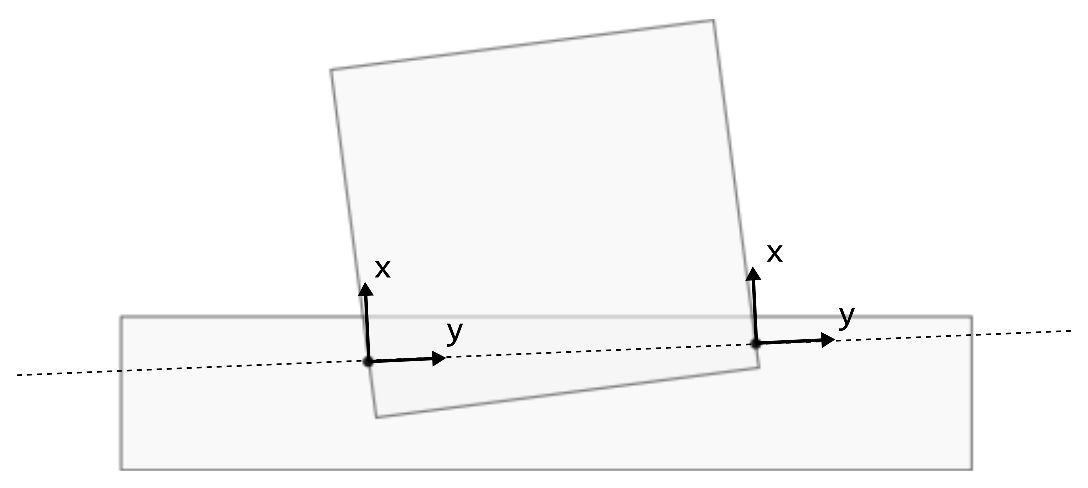
\includegraphics[clip, width=.7\hsize]{fig/phcontact.eps} \\
\end{tabular}
\end{center}
\caption{Contact configuration}
\label{fig_physics_contact}
\end{figure}

Springhead�ō̗p���Ă���ڐG���f���ɂ‚��Đ������܂��D
��\ref{sec_physics_scene}�߂ŏq�ׂ��悤�ɁC\texttt{PHSceneIf::Step}�ɂ���ăV�~�����[�V������1�X�e�b�v�i�߂�ƁC
���߂Ɍ`��̌�������ƐڐG�S���̐������s���܂��D
���������‚̌`��̌����f�ʂƁC�ڐG�S���̊֌W�ɂ‚���Fig.\,\ref{fig_physics_contact}�Ɏ����܂��D
�}�ł͊ȒP�̂��߂ɓ񎟌��ŕ`���Ă��܂����C���ۂɂ͐ڐG�f�ʂ�\�����p�`�̊e���_�ɐڐG�S��������܂��D
�ڐG�S�������̍S���Ɠ��l�Ƀ\�P�b�g�ƃv���O�ō\������܂��D
����ŁC���̍S���Ƃ͈Ⴂ�ڐG�S���͌�������A���S���Y���ɂ���ē��I�ɐ����E�j������܂��D
���̂��߁C�ڐG���������̂̂ǂ���Ƀ\�P�b�g���邢�̓v���O�����t�����邩�͏󋵈ˑ��ł���C�O������I�����邱�Ƃ͂ł��܂���D

�v���O����у\�P�b�g�̌����͎��̂悤�ɂ��Č��܂�܂��D
�܂��Cx���͐ڐG�@���ƕ��s�Ɍ����܂��D�������ǂ��炪���̌������͏󋵈ˑ��ł��D
���ɁCy���͐ڐG�_�ɂ������‚̍��̂̑��Α��x�x�N�g����ڐG�f�ʂ֓��e���������Ɍ����܂��D
�Ō��z����x�Cy���ɒ�������悤�Ɍ��܂�܂��D

�ȉ��ł͊e�ڐG�S�����ۂ������ɂ‚��ċ�̓I�ɏq�ׂ܂��D
�܂��C�@�������̐i�����x�̑召�ɉ����ďՓ˃��f���ƐÓI�ڐG���f���̂����ꂩ���I������܂��D
\begin{align*}
v^\mathrm{x} < -V^\mathrm{th}   \;\; &\Rightarrow \;\; \text{�Փ˃��f��} \\
v^\mathrm{x} \ge -V^\mathrm{th} \;\; &\Rightarrow \;\; \text{�ÓI�ڐG���f��}
\end{align*}
������$v^\mathrm{x}$�̓\�P�b�g���猩���v���O�̑��Α��x��x���i�ڐG�@���j�����ŁC�߂Â����������𕉂Ƃ��܂��D
�܂��C$V^\mathrm{th}$�͏Փ˃��f���֐؂�ւ��ՊE���x�ł��D

�Փ˃��f���ł́C1�X�e�b�v��̑��Α��x${v^\mathrm{x}}'$�����˕Ԃ�W��$e$�ɂ��ƂÂ��Č��܂�C����𖞂����悤�ȐڐG�͂��v�Z����܂��D
\begin{align}
{v^\mathrm{x}}' = - e \, v^\mathrm{x}
\end{align}
�����ŁC���˕Ԃ�W���͏Փ˂���`��̕����l�ɒ�`���ꂽ���˕Ԃ�W���̕��ϒl�ł��D
%�e�`��̒��˕Ԃ�W���́C\texttt{CDShapeDesc::e}���C\texttt{CDShapeIf::SetElasticity}��p���Đݒ肵�܂�
%�i��\ref{sec_collision_material}�ߎQ�Ɓj�D

�ÓI�ڐG���f���ł́C�`�󓯎m�̐i���[�x$d$��1�X�e�b�v�ŏ���̊����Ō�������悤�ȐڐG�͂����߂܂��D
�‚܂�C1�X�e�b�v��̐i���[�x��$d'$�Ƃ����
\begin{align}
d' = d - \gamma \mathrm{max}(d - d^\mathrm{tol}, 0)
\end{align}
�ƂȂ�܂��D
������$\gamma$�͐ڐG�S���̌덷�C�����ł��D
�܂��C$d^\mathrm{tol}$�͋��e�i���[�x�ł��D

�Ō�ɁC�ڐG�͂��������ׂ������ɂ‚��ďq�ׂ܂��D
�܂��C�@�������ɂ͔����͂̂ݍ�p���邱�Ƃ���C�ڐG�͂�x������$f^\mathrm{x}$�ɂ�
\begin{align*}
f^\mathrm{x} \ge 0
\end{align*}
���ۂ����܂��D
����ŐڐG�͂�y������$f^\mathrm{y}$�Cz������$f^\mathrm{z}$�͖��C�͂�\���܂��D
���C�͂Ɋւ��ẮC���̌����̑��Α��x�ɂ��ƂÂ��Î~���C�������C�������肳��C����ɉ����čő喀�C�͂̐��񂪉ۂ���܂��D
\begin{align*}
-\mu_0 f^\mathrm{x} \le &f^\mathrm{y} \le \mu_0 f^\mathrm{x} & & \text{if} \; -V^\mathrm{f} \le v^\mathrm{y} \le V^\mathrm{f},\\
 \mu   f^\mathrm{x} \le &f^\mathrm{y} \le \mu   f^\mathrm{x} & & \text{otherwise}
\end{align*}
�����ŁC�Î~���C�W��$\mu_0$����ѓ����C�W��$\mu$�͒��˕Ԃ�W���Ɠ��l�Ɋe�`��̕����l�̕��ϒl���p�����܂��D
�܂��C$V^\mathrm{f}$�͐Î~���C�Ɠ����C���؂�ւ��ՊE���x�ł��D
z�������ɂ‚��Ă����l�̐��񂪉ۂ���܂��D

�ڐG���f���̊֌W����C���^�t�F�[�X�ɂ͈ȉ�������܂��D
\begin{center}
\begin{longtable}{p{.1\hsize}p{.5\hsize}p{.4\hsize}}
\multicolumn{3}{l}{\texttt{CDShapeIf}}						\\ \midrule
\texttt{void}	& \texttt{SetElasticity(float e)}       & ���˕Ԃ�W����ݒ� \\
\texttt{float}  & \texttt{GetElasticity()}              & ���˕Ԃ�W�����擾 \\
\texttt{void}   & \texttt{SetStaticFriction(float mu0)} & �Ö��C�W����ݒ� \\
\texttt{float}  & \texttt{GetStaticFriction()}          & �Ö��C�W�����擾 \\
\texttt{void}   & \texttt{SetDynamicFriction(float mu)} & �����C�W����ݒ� \\
\texttt{float}  & \texttt{GetDynamicFriction()}         & �����C�W�����擾
\end{longtable}
\end{center}

\begin{center}
\begin{longtable}{p{.1\hsize}p{.5\hsize}p{.4\hsize}}
\multicolumn{3}{l}{\texttt{PHSceneIf}}						\\ \midrule
\texttt{void}	& \texttt{SetContactTolerance(double tol)} & ���e�����[�x��ݒ� \\
\texttt{double} & \texttt{GetContactTolerance()}           & ���e�����[�x���擾 \\
\texttt{void}   & \texttt{SetImpactThreshold(double vth)}  & �ŏ��Փˑ��x��ݒ� \\
\texttt{double} & \texttt{GetImpactThreshold()}            & �ŏ��Փˑ��x���擾 \\
\texttt{void}   & \texttt{SetFrictionThreshold(double vf)} & �ŏ������C���x��ݒ� \\
\texttt{double} & \texttt{GetFrictionThreshold()}          & �ŏ������C���x���擾
\end{longtable}
\end{center}

\noindent\textbf{���l}
\begin{itemize}
\item �ڐG�f�ʂ̌����ɂ‚��ẮC�`�󓯎m�̐i�����x�����ƂɌ��肵�܂����C�����ł͏ڂ����q�ׂ܂���D
\item ���C�͂Ɋւ��Ă�y���Cz�����•ʂɈ����܂����C���ۂ̖��C�͂�y������z�����̍��͂Ƃ��ė^�����܂��̂ŁC
���͂��ő喀�C�͂𒴉߂���”\��������܂��D���̂悤��Springhead�̖��C���f���͂����܂ŋߎ��I�Ȃ��̂ł��̂�
���ӂ��ĉ������D
\end{itemize}

\subsection*{�ڐG�͂̎擾}

����̍��̂ɍ�p����ڐG�͂𒼐ڎ擾���邽�߂̃C���^�t�F�[�X�͗p�ӂ���Ă��܂���D
���̂��߁C���[�U�T�C�h�ł�����x�̌v�Z���s���K�v������܂��D
�ȉ��ɁC���鍄�̂ɍ�p����ڐG�͂̍��͂����߂��������܂��D

\begin{sourcecode}
// given PHSceneIf* scene
// given PHSolidIf* solid

Vec3d fsum;    //< sum of contact forces applied to "solid"
Vec3d tsum;    //< sum of contact torques applied to "solid"

int N = scene->NContacts();
Vec3d f, t;
Posed pose;

for(int i = 0; i < N; i++){
    PHContactPointIf* con = scene->GetContact(i);
    con->GetConstraintForce(f, t);

    if(con->GetSocketSolid() == solid){
        con->GetSocketPose(pose);
        fsum -= pose.Ori() * f;
        tsum -= pose.Pos() % pose.Ori() * f;
    }
    if(con->GetPlugSolid() == solid){
        con->GetPlugPose(pose);
        fsum += pose.Ori() * f;
        tsum += pose.Pos() % pose.Ori() * f;
    }
}
\end{sourcecode}
�܂��C�V�[�����̐ڐG�S���̐���\texttt{PHSceneIf::NConstacts}�Ŏ擾���C
\texttt{for}���[�v����$i$�Ԗڂ̐ڐG�S����\texttt{PHSceneIf::GetContact}�Ŏ擾���܂��D
����\texttt{PHConstraintIf::GetConstraintForce}�ŐڐG�͂̕��i��\texttt{f}�ƃ��[�����g\texttt{t}���擾���܂����C
�ڐG�S���̏ꍇ���[�����g��$0$�ł��̂ŗp���܂���D
�܂��C������S���͂̓\�P�b�g/�v���O���W�n�ŕ\�������̂ŁC��p�_�̓\�P�b�g/�v���O���W�n�̌��_�ł��D
������l�����č��̂ɍ�p����͂ƃ��[�����g�֕ϊ����C���͂ɑ������킹�Ă����܂��D
���̂��\�P�b�g���ł���ꍇ�͍�p�E����p���l�����ĕ����𔽓]���邱�Ƃɒ��ӂ��ĉ������D


\subsection*{�ڐG�͌v�Z�̗L��/�����̐؂�ւ�}

�����̃A�v���P�[�V�����ł́C���ׂĂ̍��̂̑g�ݍ��킹�Ɋւ��ĐڐG����舵���K�v�͂���܂���D
���̂悤�ȏꍇ�͕K�v�ȍ��̂̑΂Ɋւ��Ă̂ݐڐG��L�������邱�ƂŌv�Z�R�X�g���팸�ł��܂��D
Springhead�ł́C���̂̑g�ݍ��킹���Ɍ������肨��ѐڐG�͌v�Z���s������؂�ւ��邱�Ƃ��ł��܂��D
����ɂ�\texttt{PHSceneIf::SetContactMode}��p���܂��D

\begin{center}
\begin{longtable}{p{.1\hsize}p{.9\hsize}}
\multicolumn{2}{l}{\texttt{PHSceneIf}}						\\ \midrule
\texttt{void}	& \texttt{SetContactMode(PHSolidIf* lhs, PHSolidIf* rhs, int mode)} \\
\texttt{void}   & \texttt{SetContactMode(PHSolidIf** group, size\_t length, int mode)} \\
\texttt{void}   & \texttt{SetContactMode(PHSolidIf* solid, int mode)} \\
\texttt{void}   & \texttt{SetContactMode(int mode)}
\end{longtable}
\end{center}

��Ԗڂ͍���\texttt{lhs}��\texttt{rhs}�̑΂Ɋւ��ă��[�h��ݒ肵�܂��D
��Ԗڂ͔z��\texttt{[group, group + length)}�Ɋi�[���ꂽ���̂̑S�g�ݍ��킹�Ɋւ��Đݒ肵�܂��D
�O�Ԗڂ͍���\texttt{solid}�Ƒ��̑S���̂Ƃ̑g�ݍ��킹�Ɋւ��Đݒ肵�܂��D
�l�Ԗڂ̓V�[�����̂��ׂĂ̍��̂̑g�ݍ��킹�Ɋւ��Đݒ肵�܂��D

�ݒ�”\�ȃ��[�h�͈ȉ��̓��̈�‚ł��D
\begin{center}
\begin{longtable}{p{.3\hsize}p{.7\hsize}}
\multicolumn{2}{l}{\texttt{PHSceneDesc::ContactMode}} \\ \midrule
\texttt{MODE\_NONE}	   & �������肨��ѐڐG�͌v�Z���s��Ȃ� \\
\texttt{MODE\_LCP}     & ����������s���C�S���͌v�Z�@��p���� \\
\texttt{MODE\_PENALTY} & ����������s���C�y�i���e�B���͖@��p���� \\
\end{longtable}
\end{center}
�f�t�H���g�ł͂��ׂĂ̍��̑΂Ɋւ���\texttt{MODE\_LCP}���I������Ă��܂��D
��Ƃ��āC���ʂƂ̐ڐG�ȊO�����ׂăI�t�ɂ���ɂ�
\begin{sourcecode}
// given PHSolidIf* floor

scene->SetContactMode(PHSceneDesc::MODE_NONE);
scene->SetContactMode(floor, PHSceneDesc::MODE_LCP);
\end{sourcecode}
�Ƃ��܂��D

\section{�֐ߍ��W�n�V�~�����[�V����}

\index{���񂹂‚��Ђ傤����@�֐ߍ��W�n}
T.B.D.


\section{�M�A}

\index{����@�M�A}
T.B.D.

\section{�����A���S���Y���̐ݒ�}
\label{sec_physics_engine}

�ȉ��ł͕����V�~�����[�V�����̓����ŗp�����Ă���A���S���Y���̏ڍׂȐݒ荀�ڂɂ‚��Đ������܂��D

\subsection*{�S���͌v�Z�G���W��}

�S���͌v�Z�G���W���́C�֐߂�ڐG�Ȃǂ̍S���𖞑����邽�߂̍S���͂̌v�Z���s���܂��D
�S���͌v�Z�G���W���̃N���X��\texttt{PHConstraintEngineIf}�ŁC������擾����ɂ͈ȉ��̊֐���p���܂��D


\texttt{PHConstraintEngineIf}�̃C���^�t�F�[�X���ȉ��Ɏ����܂��D

\begin{center}
\begin{longtable}{p{.12\hsize}p{.45\hsize}p{.33\hsize}}
\multicolumn{3}{l}{\texttt{PHConstraintEngineIf}}			\\ \midrule
\texttt{void}	& \texttt{SetVelCorrectionRate(double)}		& �֐ߍS���̌덷�C������ݒ� \\
\texttt{double} & \texttt{GetVelCorrectionRate()}			& �֐ߍS���̌덷�C�������擾 \\
\texttt{void}	& \texttt{SetContactCorrectionRate(double)}	& �ڐG�S���̌덷�C������ݒ� \\
\texttt{double} & \texttt{GetContactCorrectionRate()}		& �ڐG�S���̌덷�C�������擾 \\
\end{longtable}
\end{center}

�덷�C�����Ƃ́C1�X�e�b�v�ōS���덷�ǂ̒��x�C�����邩�������䗦�ŁC�ʏ�$[0, 1]$�̒l��ݒ肵�܂��D
�덷�C������$1$�ɂ���ƁC1�X�e�b�v�ōS���덷��$0$�ɂ���悤�ȍS���͂��v�Z����܂����C���U���ۂȂǂ̃V�~�����[�V�����̕s���艻�������X��������܂��D
�t�ɏC�����������ڂɐݒ肷��΃V�~�����[�V�����͈��艻���܂����C���덷�����債�܂��D

�S���͌v�Z�G���W���́C�����Ŕ����^�̃A���S���Y���ōS���͂��v�Z���܂��D
�A���S���Y���̔����񐔂�\texttt{PHSceneIf::SetNumIteration}�Őݒ肵�܂��i��\ref{sec_physics_scene}�ߎQ�Ɓj�D


\texttt{PHSceneIf::SetContactTolerance}�Őݒ�”\�ł��D

\texttt{PHConstraintEngineIf::SetContactCorrectionRate}�Őݒ�”\�ł�
�i��\ref{sec_physics_engine}�ߎQ�Ɓj�D


\chapter{Graphics}
\label{chap_graphics}
\section{�T�v}

\index{Graphics}
Graphics��3D�V�[���̕`��@�\��񋟂��郂�W���[���ł��D

\section{Graphics SDK}

\index{GRSdk}
Graphics���W���[���̂��ׂẴI�u�W�F�N�g��SDK�N���X\texttt{GRSdk}�ɂ���ĊǗ�����܂��D
\texttt{GRSdk}�N���X�́C�v���O�����̎��s��ʂ��Ă����P�‚̃I�u�W�F�N�g�����݂���V���O���g���N���X�ł��D
\texttt{GRSdk}�I�u�W�F�N�g���쐬����ɂ͈ȉ��̂悤�ɂ��܂��D
\begin{verbatim}
    GRSdkIf* grSdk = GRSdkIf::CreateSdk();
\end{verbatim}
�ʏ킱�̑���̓v���O�����̏��������Ɉ�x�������s���܂��D
�܂��CFramework���W���[�����g�p����ꍇ�̓��[�U������\texttt{GRSdk}���쐬����K�v�͂���܂���D

\texttt{GRSdk}�ɂ͈ȉ��̋@�\������܂��D
\begin{itemize}
\item �����_���̍쐬
\item �f�o�C�X�̍쐬
\item �V�[���̊Ǘ�
\end{itemize}

\index{GRRender}
\index{�����_��}
�����_���Ƃ͏����n�Ɉˑ����Ȃ����ۉ����ꂽ�`��@�\��񋟂���N���X�ł��D
�����_���̃N���X��\texttt{GRRender}�ł��D

\index{GRDeviceGL}
\index{�f�o�C�X}
����C�f�o�C�X�͏����n���Ƃ̕`�揈���̎������s���N���X�ł��D
���݂�Springhead�ł�OpenGL�ɂ��`��݂̂��T�|�[�g����Ă��܂��D
OpenGL�p�f�o�C�X�N���X��\texttt{GRDeviceGL}�ł��D

�����_�����f�o�C�X�Ɋւ���\texttt{GRSdk}�̊֐����ȉ��Ɏ����܂��D

\begin{center}
\begin{tabular}{p{.2\hsize}p{.40\hsize}p{.3\hsize}}
\texttt{GRSdkIf}		&								&	\\ \midrule
\texttt{GRRenderIf*} 	& \texttt{CreateRender()}		& �����_�����쐬		\\
\texttt{GRDeviceGLIf*} 	& \texttt{CreateDeviceGL()}		& OpenGL�f�o�C�X���쐬	\\
\end{tabular}
\end{center}

\begin{center}
\begin{tabular}{p{.2\hsize}p{.40\hsize}p{.3\hsize}}
\texttt{GRRenderIf}		&									&	\\ \midrule
\texttt{void}			& \texttt{SetDevice(GRDeviceIf*)}	& �f�o�C�X�̐ݒ�	\\
\texttt{GRDeviceIf*} 	& \texttt{GetDevice()}				& �f�o�C�X�̎擾	\\
\end{tabular}
\end{center}

\subsection*{������}

Graphics���W���[�����g�p����ɂ͈ȉ��̏�����������K�����s����K�v������܂��D
\begin{verbatim}
   	GRRenderIf* render = grSdk->CreateRender();
    GRDeviceIf* device = grSdk->CreateDeviceGL();
    device->Init();
    render->SetDevice(device);
\end{verbatim}
\texttt{GRRender}��\texttt{SetDevice}�֐��Ńf�o�C�X��o�^����ƁC�����_���͎��ۂ̕`�揈�������̃f�o�C�X��p���čs���܂��D
�����I�ɏ����n���ƂɃf�o�C�X���g�������邱�Ƃ�z�肵�C��̏����̓��[�U���s�����ƂɂȂ��Ă��܂��D
Framework���W���[�����g�p����ꍇ�̓��[�U���g�ŏ�̎葱�����s���K�v�͂���܂���D

\section{�V�[��}
\label{sec_grscene}

\subsection*{�V�[���̍쐬}

\index{GRScene}
Graphics���W���[���̃V�[���́C�R���s���[�^�O���t�B�N�X�ɂ����邢����V�[���O���t�Ɠ����̂��̂ł��D
�V�[���N���X��\texttt{GRScene}�ł��D
�V�[�����쐬����ɂ͎��̂悤�ɂ��܂��D
\begin{verbatim}
    GRSceneIf* grScene = grSdk->CreateScene();
\end{verbatim}
\texttt{GRScene}�̓f�B�X�N���v�^�ɂ��ݒ荀�ڂ������܂���D
�܂��CFig.\,\ref{fig_grscene}�Ɏ����悤��\texttt{GRSdk}�I�u�W�F�N�g�͔C�ӂ̐��̃V�[����ێ��ł��܂��D

�V�[���쐬�Ɋւ���\texttt{GRSdk}�̊֐��͈ȉ��̒ʂ�ł��D

\begin{center}
\begin{tabular}{p{.15\hsize}p{.50\hsize}p{.25\hsize}}
\texttt{GRSdkIf}	&												&	\\ \midrule
\texttt{GRSceneIf*}	& \texttt{CreateScene()}						& �V�[�����쐬			\\
\texttt{GRSceneIf*}	& \texttt{GetScene(size\_t)}					& �V�[�����擾			\\
\texttt{size\_t}	& \texttt{NScene()}								& �V�[���̐�			\\
\texttt{void}		& \texttt{MergeScene(GRSceneIf*, GRSceneIf*)}	& �V�[���̓���			\\
\end{tabular}
\end{center}

\begin{figure}[t]
\begin{center}
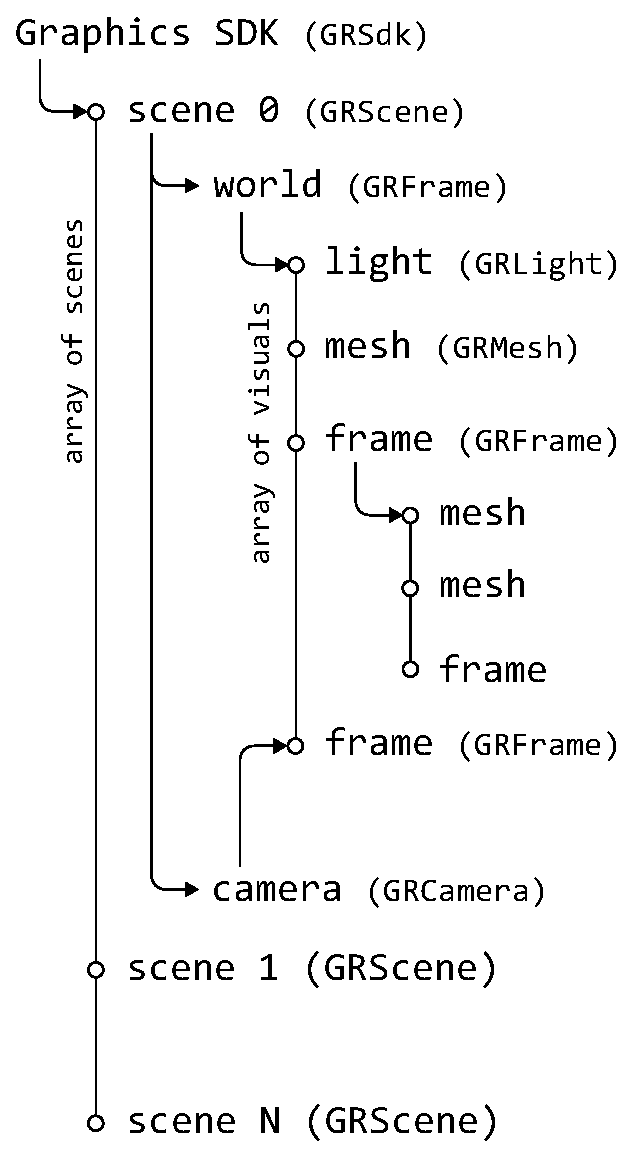
\includegraphics[width=.4\hsize]{fig/grscene.eps}
\end{center}
\caption{Graphics data structure}
\label{fig_grscene}
\end{figure}

\subsection*{�V�[���̋@�\}

�V�[�����쐬������C���͂��̃R���e���c�ł���t���[���⃁�b�V���C�J�����⃉�C�g�Ȃǂ��쐬���ăV�[���ɉ����Ă����܂��D
���̕��@�Ƃ��Ă͊��S�Ɏ蓮�ŃV�[�����\�z���鑼�ɂ�FileIO���W���[�����g�p���ăt�@�C������V�[�������[�h������@������܂��D
�ȉ���\texttt{GRScene}�̊֐��������܂��D

\begin{center}
\begin{tabular}{p{.15\hsize}p{.45\hsize}p{.3\hsize}}
\texttt{GRSceneIf}	 &															&	\\ \midrule
\texttt{GRFrameIf*}	 & \texttt{GetWorld()}										& ���[���h�t���[���̎擾	\\
\texttt{GRCameraIf*} & \texttt{GetCamera()}										& �J�����̎擾	\\
\texttt{void}		 & \texttt{SetCamera(const GRCameraDesc\&)}					& �J�����̐ݒ�	\\
\texttt{GRVisualIf*} & \texttt{CreateVisual(const GRVisualDesc\&, GRFrameIf*)}	& �`��A�C�e���̍쐬	\\
\texttt{void}		 & \texttt{Render(GRRenderIf*)}								& �`��	\\
\end{tabular}
\end{center}

%	///	�A�j���[�V�����R���g���[���̎擾
%	GRAnimationControllerIf* GetAnimationController();

Fig.\,\ref{fig_grscene}�Ɏ����悤�ɁC1�‚̃V�[���͂���1�‚̃��[���h�t���[���������C�������_�Ƃ���
�C�ӂ̐��̕`��A�C�e�����c���[��ɘA�Ȃ�܂��D
���[���h�t���[����\texttt{GetWorld}�Ŏ擾���܂��D

����ȕ`��A�C�e���ɃJ����������܂��D
�J�����̓��[���h�t���[���ȉ��̃c���[�Ƃ͕ʂɁC\texttt{GRScene}���ێ����܂�(Fig.\,\ref{fig_grscene})�D
�J�����̐ݒ��\texttt{SetCamera}�ōs���܂��D
�J�������擾����ɂ�\texttt{GetCamera}���g���܂��D
�܂��C�J�����̓V�[���O���t����1�‚̃t���[�����Q�Ƃ��C��������_�̐ݒ�ɗp���܂��D
�C���[�W�Ƃ��Ă̓J�������Q�Ɛ�̃t���[���Ɏ��t�����Ă���ƍl����������R�ł��傤�D
�Q�Ɛ�̃t���[���̈ړ��ɉ����ăJ�������V�[�������ړ����邱�ƂɂȂ�܂��D


\subsection*{�V�[���̕`��}

�`�揈���̓v���O�����̕`��n���h���ōs���܂��DGLUT���g���ꍇ��\texttt{glutDisplayFunc}�œo�^�����R�[���o�b�N�֐�������ɂ�����C
�܂�Framework���W���[����\texttt{FWApp}���g���ꍇ��\texttt{Display}���z�֐�������ɂ�����܂��D
�ȉ����T�^�I�ȕ`�揈���ł��D
\begin{verbatim}
    render->ClearBuffer();        // clear back buffer
    render->BeginScene();         // begin rendering

    grScene->Render(render);      // render scene

    render->EndScene();           // end rendering
    render->SwapBuffers();        // swap buffers
\end{verbatim}

\texttt{ClearBuffer}�͕`��o�b�t�@������̐F�œh��‚Ԃ��܂��D
�h��‚Ԃ��F�̎擾/�ݒ��\texttt{GRRender}��\texttt{GetClearColor}�C\text{SetClearColor}���g���܂��D
\begin{verbatim}
    render->SetClearColor(Vec4f(1.0f, 0.0f, 0.0f, 1.0f));
    render->ClearBuffer();        // clear back buffer in red
\end{verbatim}

\texttt{BeginScene}��\texttt{EndScene}�̓V�[���̕`��̑O��ŕK���Ăяo���܂��D
\texttt{SwapBuffers}�̓t�����g�o�b�t�@�ƃo�b�N�o�b�t�@��؂芷���邱�Ƃŕ`����e����ʏ�ɕ\�����܂��D

\texttt{GRScene}��\texttt{Render}�֐��́C�J����(\texttt{GRCamera})��\texttt{Render}�ƃ��[���h�t���[��(\texttt{GRFrame})��\texttt{Render}��
�����Ăяo���܂��D�܂��J�����̕`��ɂ���Ď��_�Ɠ��e�ϊ����ݒ肳��C
���Ƀ��[���h�t���[���̕`��ɂ���ăV�[���O���t���ċA�I�ɕ`�悳��܂��D

\section{�`��A�C�e��}

\begin{figure}[t]
\begin{center}
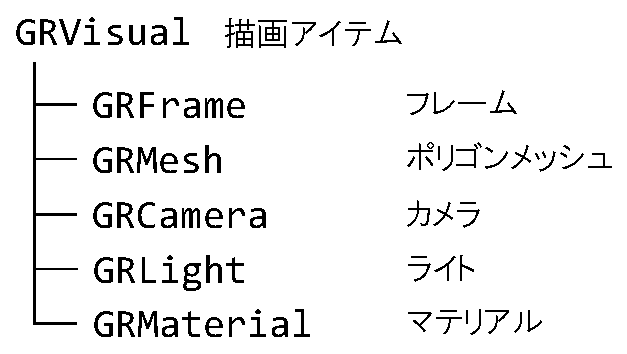
\includegraphics[width=.4\hsize]{fig/grvisual.eps}
\end{center}
\caption{Class hierarchy of visual items}
\label{fig_grvisual}
\end{figure}

\index{GRVisual}
�V�[���O���t���\������`��A�C�e���̊�{�N���X��\texttt{GRVisual}�ł��D
\texttt{GRVisual}����h������N���X��Fig.\,\ref{fig_grvisual}�Ɏ����܂��D
�`��A�C�e���ɂ͈ȉ��̋��ʂ̋@�\������܂��D

\begin{center}
\begin{tabular}{p{.15\hsize}p{.45\hsize}p{.3\hsize}}
\multicolumn{3}{l}{\texttt{GRVisualIf}}					\\ \midrule
\texttt{void}	& \texttt{Render(GRRenderIf*)}		& 	\\
\texttt{void} 	& \texttt{Rendered(GRRenderIf*)}	& 	\\
\texttt{void} 	& \texttt{Enable(bool)}				& 	\\
\texttt{bool} 	& \texttt{IsEnabled()}				& 	\\
\end{tabular}
\end{center}

\texttt{Render}�̓A�C�e���̕`����s���C\texttt{Rendered}�͕`��̌㏈�����s���܂��D
�`�揈���͕`��A�C�e���̎�ނ��ƂɈقȂ�܂��D
����ɂ‚��Ă͎��߈ȍ~�Ő������܂��D

\texttt{Enable}�֐��͕`�揈���̗L����/���������s���܂��D
���������ꂽ�A�C�e���͕`�悳��܂���D
\texttt{IsEnabled}�֐��͗L��/������Ԃ�Ԃ��܂��D

�`��A�C�e�����쐬����ɂ�\texttt{GRScene}��\texttt{CreateVisual}�֐��Ɏ�ނ��Ƃ̃f�B�X�N���v�^���w�肵�ČĂяo���܂��D


\section{�t���[��}

\index{GRFrame}
\index{�ӂ�[��@�t���[��}
�t���[���͍��W�ϊ����`����Ɠ����ɑ��̕`��A�C�e���̃R���e�i�Ƃ��Ă̖����������܂��D
�t���[���̃N���X��\texttt{GRFrame}�ł��D
���̃R�[�h�́C�t���[�����쐬���ă��[���h�t���[���̎q�Ƃ��ēo�^���܂��D
\begin{verbatim}
    GRFrameDesc desc;
    GRFrameIf* frame =
        grScene->CreateVisual(desc, grScene->GetWorldFrame())->Cast();
\end{verbatim}
\texttt{CreateVisual}�֐��͎w�肳�ꂽ�f�B�X�N���v�^�ɑΉ�����`��A�C�e�����쐬���C
�w�肳�ꂽ�e�t���[���̎q�Ƃ��ēo�^���܂��D�e�t���[�����Ȃ��ƃf�t�H���g�Ń��[���h�t���[���ɓo�^����܂��D
���������ď�̃R�[�h��\texttt{CreateVisual(desc)}�Ƃ��Ă����܂��܂���D

\texttt{GRFrame}��\texttt{Render}�֐��́C�q�`��A�C�e����\texttt{Render}�������Ăяo���܂��D


\subsection*{�e�q�֌W}

�t���[���Ԃ̐e�q�֌W���Ǘ�����֐��ɂ͎��̂��̂�����܂��D

\begin{center}
\begin{tabular}{p{.20\hsize}p{.45\hsize}p{.25\hsize}}
\multicolumn{3}{l}{\texttt{GRFrameIf}}						\\ \midrule
\texttt{GRFrameIf*}		& \texttt{GetParent()}				& 	\\
\texttt{void} 			& \texttt{SetParent(GRFrameIf*)}	& 	\\
\texttt{int} 			& \texttt{NChildren()}				& 	\\
\texttt{GRVisualIf**} 	& \texttt{GetChildren()}			& 	\\
\end{tabular}
\end{center}

\texttt{GetParent}�͐e�t���[�����擾���܂��D
\texttt{SetParent}�͂��̃t���[���̐e�t���[����ύX���邽�߂Ɏg���܂��D
\texttt{NChildren}�͂��̃t���[���̎q�ł���`��A�C�e���̐���Ԃ��܂��D
�����ɂ̓t���[���ȊO�̕`��A�C�e�����܂܂�邱�Ƃɒ��ӂ��Ă��������D
\texttt{GetChildren}�͎q�`��A�C�e���̔z����擾���܂��D


\subsection*{���W�ϊ�}

�t���[���̍��W�ϊ��𑀍삷��֐��͈ȉ��̒ʂ�ł��D

\begin{center}
\begin{tabular}{p{.15\hsize}p{.45\hsize}p{.3\hsize}}
\multicolumn{3}{l}{\texttt{GRFrameIf}}							\\ \midrule
\texttt{Affinef} & \texttt{GetTransform()}					& 	\\
\texttt{Affinef} & \texttt{GetWorldTransform()}				& 	\\
\texttt{void}	 & \texttt{SetTransform(const Affinef\&)}	& 	\\
\end{tabular}
\end{center}

\texttt{GetTransform}�C\texttt{SetTransform}�͂��ꂼ��t���[���Ƃ��̐e�t���[���Ƃ̊Ԃ̑��ΓI�ȍ��W�ϊ����擾/�ݒ肵�܂��D
�Ⴆ��
\begin{verbatim}
    frame->SetTransform(Affinef::Trn(1.0, 0.0, 0.0));
\end{verbatim}
�Ƃ���Ɛe�t���[���ɑ΂��đ��ΓI��x������$1.0$�ړ����܂��D

\section{�J����}

\begin{figure}[t]
\begin{tabular}{c}
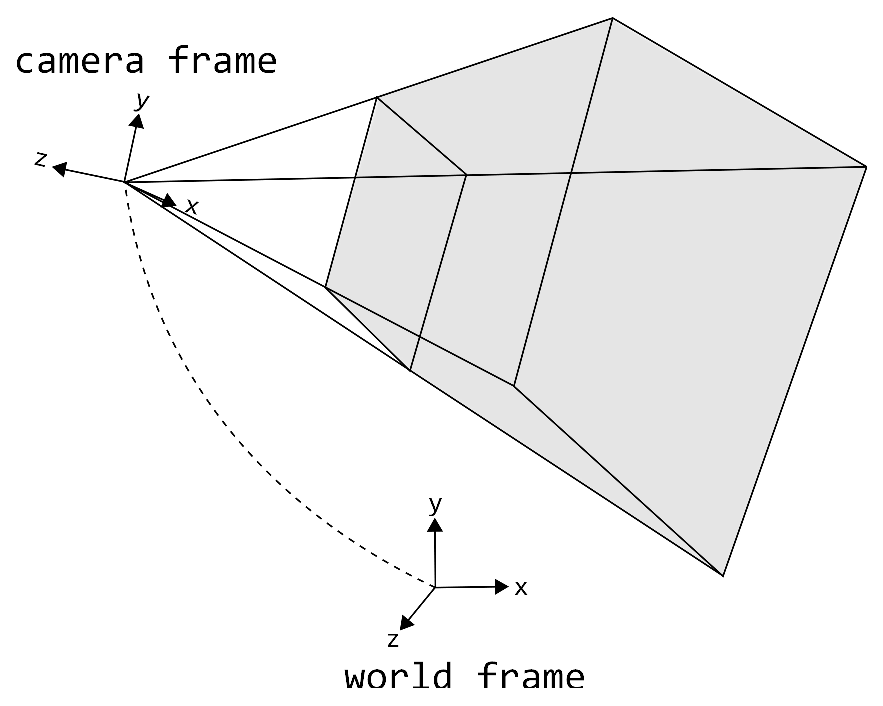
\includegraphics[width=.4\hsize]{fig/grcamera.eps} \\
(a) Perspective frustum \\
\\
\begin{tabular}{cc}
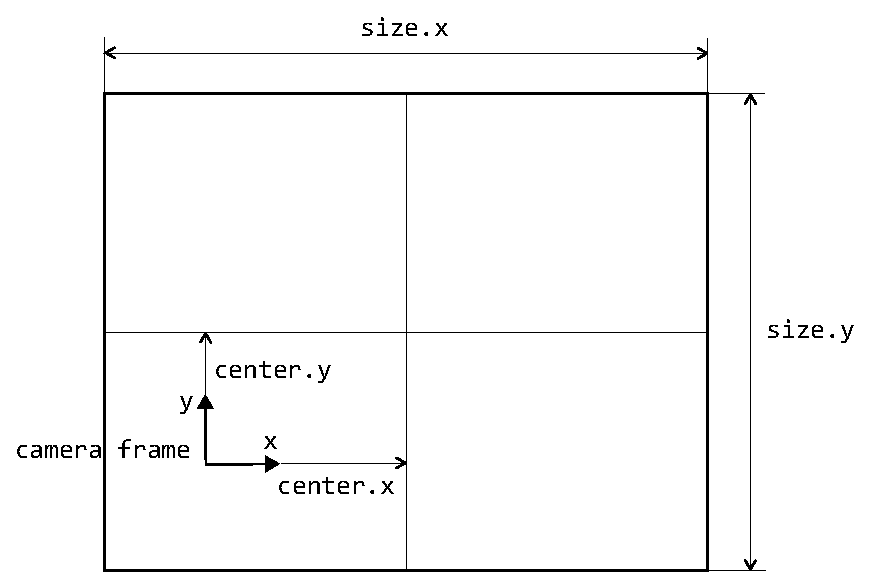
\includegraphics[width=.4\hsize]{fig/grcamera_front.eps} &
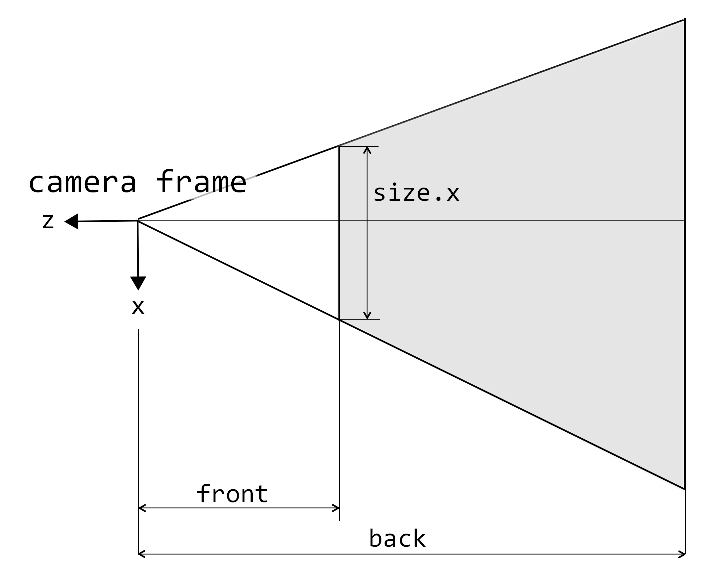
\includegraphics[width=.4\hsize]{fig/grcamera_top.eps} \\
(b) Front view of screen &
(c) Top view of screen
\end{tabular}
\end{tabular}
\caption{Camera parameters}
\label{fig_grcamera}
\end{figure}

\index{GRCamera}
\index{���߂�@�J����}
�J�����͕`��ɂ����鎋�_�̐ݒ�Ɠ��e�ϊ����Ǘ����܂��D
�͂��߂ɃJ�����̃f�B�X�N���v�^�����Ă����܂��D

\begin{center}
\begin{tabular}{p{.15\hsize}p{.45\hsize}p{.3\hsize}}
\multicolumn{3}{l}{\texttt{GRCameraDesc}}					\\ \midrule
\texttt{Vec2f}	&	\texttt{size}	& �X�N���[���T�C�Y 		\\
\texttt{Vec2f}	&	\texttt{center}	& �X�N���[�����S���W 	\\
\texttt{float}	&	\texttt{front}	& �O���N���b�v��		\\
\texttt{float}	&	\texttt{back}	& ����N���b�v��		\\
\end{tabular}
\end{center}

�e�ϐ��̒�`��Fig.\,\ref{fig_grcamera}(b),(c)���Q�Ƃ��Ă��������D
�ݒ��ύX����ɂ͈ȉ��̂悤�ɂ��܂��D
\begin{verbatim}
    GRCameraDesc desc;
    grScene->GetCamera()->GetDesc(&desc);
    desc.front = 3.0f;
    grScene->SetCamera(desc);
\end{verbatim}
��ł�\texttt{GetDesc}�֐��Ŋ����̐ݒ���f�B�X�N���v�^�ɃR�s�[���C\texttt{front}��ύX���Ă���
\texttt{SetCamera}�֐��ōĐݒ肵�Ă��܂��D

����C\texttt{GRCamera}�̊֐��͈ȉ��̒ʂ�ł��D

\begin{center}
\begin{tabular}{p{.15\hsize}p{.45\hsize}p{.3\hsize}}
\multicolumn{3}{l}{\texttt{GRCameraIf}}					\\ \midrule
\texttt{GRFrameIf*}	& \texttt{GetFrame()}				&	\\
\texttt{void}		& \texttt{SetFrame(GRFrameIf*)}		&	\\
\end{tabular}
\end{center}

\texttt{GetFrame}�C\texttt{SetFrame}�֐��̓J�����t���[�����擾/�ݒ肵�܂��D
Fig.\,\ref{fig_grcamera}(a)�̂悤�ɁC�J�����t���[���̓J�����̎��_���`���܂��D

\section{���C�g}

\index{GRLight}
\index{�炢��@���C�g}
���C�g�̓V�[���̏Ɩ���ݒ肷�邽�߂̕`��A�C�e���ł��D
���C�g�̃N���X\texttt{GRLight}�̃f�B�X�N���v�^�̑�\�I�ȕϐ����ȉ��Ɏ����܂��D

\begin{center}
\begin{tabular}{p{.15\hsize}p{.45\hsize}p{.3\hsize}}
\multicolumn{3}{l}{\texttt{GRLightDesc}}				\\ \midrule
\texttt{Vec4f}	&	\texttt{ambient}	& �‹��� 		\\
\texttt{Vec4f}	&	\texttt{diffuse}	& �g�U�� 		\\
\texttt{Vec4f}	&	\texttt{specular}	& ���ʌ�		\\
\texttt{Vec4f}	&	\texttt{position}	& ���C�g�ʒu	\\
\end{tabular}
\end{center}

�����W����X�|�b�g���C�g�Ȃǂ̂��ڍׂȐݒ荀�ڂɂ‚��Ă̓\�[�X�t�@�C�����Q�Ƃ��Ă��������D
OpenGL�̎d�l�Ɠ��l�C\texttt{position}�̑�4����\texttt{position.w}��$0$�̏ꍇ�͕��s�����ƂȂ�C
\texttt{(x,y,z)}�����̖������Ƀ��C�g�����邱�ƂɂȂ�C\texttt{position.w}��$1$�̏ꍇ��
\texttt{(x,y,z)}�̈ʒu�ɓ_������������܂��D

\section{�}�e���A��}
\label{sec_grmaterial}

\index{GRMaterial}
\index{�܂Ă肠��@�}�e���A��}
�}�e���A���͍ގ����w�肷�邽�߂̃A�C�e���ł��D
�}�e���A���̃N���X��\texttt{GRMaterial}�ł��D
�ʏ�C�}�e���A���͎��߂Ő������郁�b�V���̎q�`��A�C�e���ƂȂ�܂��D
�t�@�C�����烁�b�V�������[�h����ꍇ�́C���b�V���̍쐬�Ɠ����Ƀ}�e���A���������I�ɍ쐬����C���b�V���̎q�Ƃ��Ēlj�����܂��D
\texttt{GRMaterial}�̃f�B�X�N���v�^�͈ȉ��̒ʂ�ł��D

\begin{center}
\begin{tabular}{p{.15\hsize}p{.45\hsize}p{.3\hsize}}
\multicolumn{3}{l}{\texttt{GRMaterialDesc}}				\\ \midrule
\texttt{Vec4f}		&	\texttt{ambient}	& �‹��F 	\\
\texttt{Vec4f}		&	\texttt{diffuse}	& �g�U�F 	\\
\texttt{Vec4f}		&	\texttt{specular}	& ���ʐF	\\
\texttt{Vec4f}		&	\texttt{emissive}	& ���Ȕ���	\\
\texttt{float}		&	\texttt{power}		& ���ʌW��	\\
\texttt{UTString}	&	\texttt{texname}	& �e�N�X�`���t�@�C����
\end{tabular}
\end{center}

�����_���Ƀ}�e���A����ݒ肷��ƁC���ɕʂ̃}�e���A����ݒ肷��܂ł̊Ԃ�
�`��`��ɂ��̃}�e���A���̕`�摮�����K�p����܂��D
�}�e���A����ݒ肷��ɂ͂����‚��̕��@������܂��D
��–ڂ�\texttt{GRMaterialIf}��\texttt{Render}�֐����Ăԕ��@�ł�:
����ɉ����C�ȉ��Ɏ���\texttt{GRRender}�̊֐��̂����ꂩ��p���邱�Ƃ��ł��܂��D
\begin{center}
\begin{tabular}{p{.1\hsize}p{.5\hsize}p{.3\hsize}}
\texttt{GRRenderIf}																\\ \midrule
\texttt{void} & \texttt{SetMaterial(const GRMaterialDesc\&)}		& �`��}�e���A���̐ݒ�	\\
\texttt{void} & \texttt{SetMaterial(const GRMaterialIf*)}			& �`��}�e���A���̐ݒ�	\\
\texttt{void} & \texttt{SetMaterial(int)}							& �`��}�e���A���̐ݒ�	\\
\end{tabular}
\end{center}
�ȉ��̗�̓}�e���A����ݒ肷��3�ʂ�̕��@�������Ă��܂��D
�ǂ̕��@��p���Ă����ʂ͕ς��܂���D
\begin{verbatim}
    // given GRRenderIf* render, GRSceneIf* scene
    GRMaterialDesc md;
    md.diffuse = Vec4f(1.0f, 0.0f, 0.0f, 1.0f);
    // 1.
    render->SetMaterial(md);
    // 2.
    GRMaterialIf* mat = scene->CreateVisual(md)->Cast();
    mat->Render(render);
    // 3.
    render->SetMaterial(mat);
\end{verbatim}
����}�e���A�����쐬����͔̂ς킵�����Ƃ�����܂��D
���̂悤�ȏꍇ�̓����_���̗\��F���w�肷�邱�Ƃ��”\�ł��D
\begin{verbatim}
    // 4.
    render->SetMaterial(GRRenderBaseIf::RED);
\end{verbatim}
�g�p�”\�ȗ\��F��X11 web color�ɂ��ƂÂ��Ă��܂��D
�ڂ�����\texttt{SprGRRender.h}�w�b�_�t�@�C����

%%%%%%%%%%%%%%%%%%%%%%%%%%%%%%%%%%%%%%%%%%%%%%%%%%%%%%%%%%%%%%%%%%%%%%%%%%%%%%%%%%%%%%
\begin{comment}

\begin{table}[t]
\caption{Reserved colors}
\label{table_material_sample}
{\small
\begin{center}
\begin{tabular}{ll|ll}
RED				& {\color[RGB]{255,0,0}$\blacksquare$} 			(1.00, 0.00, 0.00)	&
GREEN			& {\color[rgb]{0,1,0}$\blacksquare$} 			(0.00, 1.00, 0.00)	\\
BLUE			& {\color[rgb]{0,0,1}$\blacksquare$} 			(0.00, 0.00, 1.00)	&
YELLOW			& {\color[rgb]{1,1,0}$\blacksquare$} 			(1.00, 1.00, 0.00)	\\
CYAN			& {\color[rgb]{0,1,1}$\blacksquare$} 			(0.00, 1.00, 1.00)	&
MAGENTA			& {\color[rgb]{1,0,1}$\blacksquare$} 			(1.00, 0.00, 1.00)	\\
WHITE			& {$\square$} 						 			(1.00, 1.00, 1.00)	&
GRAY			& {\color[rgb]{.5,.5,.5}$\blacksquare$} 		(0.50, 0.50, 0.50)	\\
ORANGE			& {\color[rgb]{1,.27,0}$\blacksquare$} 			(1.00, 0.27, 0.00)	&
BROWN			& {\color[rgb]{.198,0,0}$\blacksquare$} 		(0.19, 0.00, 0.00)	\\
LIGHT\_BLUE		& {\color[rgb]{.676,.844,.898}$\blacksquare$} 	(0.67, 0.84, 0.89)	&
MEDIUM\_PURPLE	& {\color[rgb]{.574,.438,.855}$\blacksquare$} 	(0.57, 0.43, 0.85)	\\
DARK\_GREEN		& {\color[rgb]{0,.391,0}$\blacksquare$} 		(0.00, 0.39, 0.00)	&
DARK\_VIOLET	& {\color[rgb]{.578,0,.824}$\blacksquare$} 		(0.57, 0.00, 0.82)	\\
DARK\_CYAN		& {\color[rgb]{0,.543,.543}$\blacksquare$} 		(0.00, 0.54, 0.54)	&
GREEN\_YELLOW	& {\color[rgb]{.676,1,.184}$\blacksquare$} 		(0.67, 1.00, 0.18)	\\
LIME\_GREEN		& {\color[rgb]{.195,.801,.195}$\blacksquare$} 	(0.19, 0.80, 0.19)	&
INDIAN\_RED		& {\color[rgb]{.801,.359,.359}$\blacksquare$} 	(0.80, 0.35, 0.35)	\\
INDIGO			& {\color[rgb]{.293,0,.508}$\blacksquare$} 		(0.29, 0.00, 0.50)	&
GREEN\_INDIGO	& {\color[rgb]{0,.198,.198}$\blacksquare$} 		(0.00, 0.19, 0.19)	\\
OLIVE\_GREEN	& {\color[rgb]{.198,.398,0}$\blacksquare$} 		(0.19, 0.39, 0.00)	&
NAVY\_BLUE		& {\color[rgb]{.198,.398,.797}$\blacksquare$} 	(0.19, 0.39, 0.79)	\\
TURQUOISE\_BLUE	& {\color[rgb]{.398,1,.797}$\blacksquare$} 		(0.39, 1.00, 0.79)	&
EMERALD\_GREEN	& {\color[rgb]{.598,1,.398}$\blacksquare$} 		(0.59, 1.00, 0.39)
\end{tabular}
\end{center}
}
\end{table}

\end{comment}
%%%%%%%%%%%%%%%%%%%%%%%%%%%%%%%%%%%%%%%%%%%%%%%%%%%%%%%%%%%%%%%%%%%%%%%%%%%%%%%%%%%%%%

\begin{table}[t]
\caption{Reserved colors}
\label{table_material_sample}
{\tiny
\begin{center}
\ifLwarp\else
\begin{tabular}{l|l}
\fi
\begin{tabular}{lll}
INDIANRED		& {\color[RGB]{205,92,92}$\blacksquare$}	& (205 92 92) \\
LIGHTCORAL		& {\color[RGB]{240,128,128}$\blacksquare$}	& (240 128 128) \\
SALMON			& {\color[RGB]{250,128,114}$\blacksquare$}	& (250 128 114) \\
DARKSALMON		& {\color[RGB]{233,150,122}$\blacksquare$}	& (233 150 122) \\
LIGHTSALMON		& {\color[RGB]{255,160,122}$\blacksquare$}	& (255 160 122) \\
RED				& {\color[RGB]{255,0,0}$\blacksquare$}		& (255 0 0) \\
CRIMSON			& {\color[RGB]{220,20,60}$\blacksquare$}	& (220 20 60) \\
FIREBRICK		& {\color[RGB]{178,34,34}$\blacksquare$}	& (178 34 34) \\
DARKRED			& {\color[RGB]{139,0,0}$\blacksquare$}		& (139 0 0) \\
\\
PINK			& {\color[RGB]{255,192,203}$\blacksquare$}	& (255 192 203)	\\
LIGHTPINK		& {\color[RGB]{255,182,193}$\blacksquare$}	& (255 182 193)	\\
HOTPINK			& {\color[RGB]{255,105,180}$\blacksquare$}	& (255 105 180)	\\
DEEPPINK		& {\color[RGB]{255, 20,147}$\blacksquare$}	& (255  20 147)	\\
MEDIUMVIOLETRED	& {\color[RGB]{199, 21,133}$\blacksquare$}	& (255  21 133)	\\
PALEVIOLETRED	& {\color[RGB]{219,112,147}$\blacksquare$}	& (255 112 147)	\\
\\
CORAL			& {\color[RGB]{255,127, 80}$\blacksquare$}	& (255 127 80)	\\
TOMATO			& {\color[RGB]{255, 99, 71}$\blacksquare$}	& (255  99 71)	\\
ORANGERED		& {\color[RGB]{255, 69,  0}$\blacksquare$}	& (255  69 0)	\\
DARKORANGE		& {\color[RGB]{255,140,  0}$\blacksquare$}	& (255 140 0)	\\
ORANGE			& {\color[RGB]{255,165,  0}$\blacksquare$}	& (255 165 0)	\\
\\
GOLD					& {\color[RGB]{255,215,0}$\blacksquare$}	& (255 215 0)	\\
YELLOW					& {\color[RGB]{255,255,0}$\blacksquare$}	& (255 255 0)	\\
LIGHTYELLOW				& {\color[RGB]{255,255,224}$\blacksquare$}	& (255 255 224)	\\
LEMONCHIFFON			& {\color[RGB]{255,250,205}$\blacksquare$}	& (255 250 205)	\\
LIGHTGOLDENRODYELLOW	& {\color[RGB]{250,250,210}$\blacksquare$}	& (250 250 210)	\\
PAPAYAWHIP				& {\color[RGB]{255,239,213}$\blacksquare$}	& (255 239 213)	\\
MOCCASIN				& {\color[RGB]{255,228,181}$\blacksquare$}	& (255 228 181)	\\
PEACHPUFF				& {\color[RGB]{255,218,185}$\blacksquare$}	& (255 218 185)	\\
PALEGOLDENROD			& {\color[RGB]{238,232,170}$\blacksquare$}	& (238 232 170)	\\
KHAKI					& {\color[RGB]{240,230,140}$\blacksquare$}	& (240 230 140)	\\
DARKKHAKI				& {\color[RGB]{189,183,107}$\blacksquare$}	& (189 183 107)	\\
\\						
LAVENDAR				& {\color[RGB]{230,230,250}$\blacksquare$}	& (230 230 250)	\\
THISTLE					& {\color[RGB]{216,191,216}$\blacksquare$}	& (216 191 216)	\\
PLUM					& {\color[RGB]{221,160,221}$\blacksquare$}	& (221 160 221)	\\
VIOLET					& {\color[RGB]{238,130,238}$\blacksquare$}	& (238 130 238)	\\
ORCHILD					& {\color[RGB]{218,112,214}$\blacksquare$}	& (218 112 214)	\\
FUCHSIA					& {\color[RGB]{255,0,255}$\blacksquare$}	& (255 0 255)	\\
MAGENTA					& {\color[RGB]{255,0,255}$\blacksquare$}	& (255 0 255)	\\
MEDIUMORCHILD			& {\color[RGB]{186,85,211}$\blacksquare$}	& (186 85 211)	\\
MEDIUMPURPLE			& {\color[RGB]{147,112,219}$\blacksquare$}	& (147 112 219)	\\
BLUEVIOLET				& {\color[RGB]{138,43,226}$\blacksquare$}	& (138 43 226)	\\
DARKVIOLET				& {\color[RGB]{148,0,211}$\blacksquare$}	& (148 0 211)	\\
DARKORCHILD				& {\color[RGB]{153,50,204}$\blacksquare$}	& (153 50 204)	\\
DARKMAGENTA				& {\color[RGB]{139,0,139}$\blacksquare$}	& (139 0 139)	\\
PURPLE					& {\color[RGB]{128,0,128}$\blacksquare$}	& (128 0 128)	\\
INDIGO					& {\color[RGB]{75,0,130}$\blacksquare$}	& (75 0 130)	\\
DARKSLATEBLUE			& {\color[RGB]{72,61,139}$\blacksquare$}	& (72 61 139)	\\
SLATEBLUE				& {\color[RGB]{106,90,205}$\blacksquare$}	& (106 90 205)	\\
MEDIUMSLATEBLUE			& {\color[RGB]{123,104,238}$\blacksquare$}	& (123 104 238)	\\
\\
GREENYELLOW				& {\color[RGB]{173,255,47}$\blacksquare$}	& (173 255 47)	\\
CHARTREUSE				& {\color[RGB]{127,255,0}$\blacksquare$}	& (127 255 0)	\\
LAWNGREEN				& {\color[RGB]{124,252,0}$\blacksquare$}	& (124 252 0)	\\
LIME					& {\color[RGB]{0,255,0}$\blacksquare$}	& (0 255 0)	\\
LIMEGREEN				& {\color[RGB]{50,205,50}$\blacksquare$}	& (50 205 50)	\\
PALEGREEN				& {\color[RGB]{152,251,152}$\blacksquare$}	& (152 251 152)	\\
LIGHTGREEN				& {\color[RGB]{144,238,144}$\blacksquare$}	& (144 238 144)	\\
MEDIUMSPRINGGREEN		& {\color[RGB]{0,250,154}$\blacksquare$}	& (0 250 154)	\\
SPRINGGREEN				& {\color[RGB]{0,255,127}$\blacksquare$}	& (0 255 127)	\\
MEDIUMSEAGREEN			& {\color[RGB]{60,179,113}$\blacksquare$}	& (60 179 113)	\\
SEAGREEN				& {\color[RGB]{46,139,87}$\blacksquare$}	& (46 139 87)	\\
FORESTGREEN				& {\color[RGB]{34,139,34}$\blacksquare$}	& (34 139 34)	\\
GREEN					& {\color[RGB]{0,128,0}$\blacksquare$}	& (0 128 0)	\\
DARKGREEN				& {\color[RGB]{0,100,0}$\blacksquare$}	& (0 100 0)	\\
YELLOWGREEN				& {\color[RGB]{154,205,50}$\blacksquare$}	& (154 205 50)	\\
OLIVEDRAB				& {\color[RGB]{107,142,35}$\blacksquare$}	& (107 142 35)	\\
OLIVE					& {\color[RGB]{128,128,0}$\blacksquare$}	& (128 128 0)	\\
DARKOLIVEGREEN			& {\color[RGB]{85,107,47}$\blacksquare$}	& (85 107 47)	\\
MEDIUMAQUAMARINE		& {\color[RGB]{102,205,170}$\blacksquare$}	& (102 205 170)	\\
DARKSEAGREEN			& {\color[RGB]{143,188,143}$\blacksquare$}	& (143 188 143)	\\
LIGHTSEAGREEN			& {\color[RGB]{32,178,170}$\blacksquare$}	& (32 178 170)	\\
DARKCYAN				& {\color[RGB]{0,139,139}$\blacksquare$}	& (0 139 139)	\\
TEAL					& {\color[RGB]{0,128,128}$\blacksquare$}	& (0 128 128)	\\
\\
\end{tabular}
\ifLwarp\vspace{2\baselineskip}\else
&
\fi
\begin{tabular}{lll}
AQUA				& {\color[RGB]{0,255,255}$\blacksquare$}	& (0 255 255)	\\
CYAN				& {\color[RGB]{0,255,255}$\blacksquare$}	& (0 255 255)	\\
LIGHTCYAN			& {\color[RGB]{224,255,255}$\blacksquare$}	& (224 255 255)	\\
PALETURQUOISE		& {\color[RGB]{175,238,238}$\blacksquare$}	& (175 238 238)	\\
AQUAMARINE			& {\color[RGB]{127,255,212}$\blacksquare$}	& (127 255 212)	\\
TURQUOISE			& {\color[RGB]{64,224,208}$\blacksquare$}	& (64 224 208)	\\
MEDIUMTURQUOISE		& {\color[RGB]{72,209,204}$\blacksquare$}	& (72 209 204)	\\
DARKTURQUOISE		& {\color[RGB]{0,206,209}$\blacksquare$}	& (0 206 209)	\\
CADETBLUE			& {\color[RGB]{95,158,160}$\blacksquare$}	& (95 158 160)	\\
STEELBLUE			& {\color[RGB]{70,130,180}$\blacksquare$}	& (70 130 180)	\\
LIGHTSTEELBLUE		& {\color[RGB]{176,196,222}$\blacksquare$}	& (176 196 222)	\\
POWDERBLUE			& {\color[RGB]{176,224,230}$\blacksquare$}	& (176 224 230)	\\
LIGHTBLUE			& {\color[RGB]{173,216,230}$\blacksquare$}	& (173 216 230)	\\
SKYBLUE				& {\color[RGB]{135,206,235}$\blacksquare$}	& (135 206 235)	\\
LIGHTSKYBLUE		& {\color[RGB]{135,206,250}$\blacksquare$}	& (135 206 250)	\\
DEEPSKYBLUE			& {\color[RGB]{0,191,255}$\blacksquare$}	& (0 191 255)	\\
DODGERBLUE			& {\color[RGB]{30,144,255}$\blacksquare$}	& (30 144 237)	\\
CORNFLOWERBLUE		& {\color[RGB]{100,149,237}$\blacksquare$}	& (65 105 225)	\\
ROYALBLUE			& {\color[RGB]{65,105,225}$\blacksquare$}	& (65 105 225)	\\
BLUE				& {\color[RGB]{0,0,255}$\blacksquare$}	& (0 0 255)	\\
MEDIUMBLUE			& {\color[RGB]{0,0,205}$\blacksquare$}	& (0 0 205)	\\
DARKBLUE			& {\color[RGB]{0,0,139}$\blacksquare$}	& (0 0 139)	\\
NAVY				& {\color[RGB]{0,0,128}$\blacksquare$}	& (0 0 128)	\\
MIDNIGHTBLUE		& {\color[RGB]{25,25,112}$\blacksquare$}	& (25 25 112)	\\
\\
CORNSILK			& {\color[RGB]{255,248,220}$\blacksquare$}	& (255 248 220)	\\
BLANCHEDALMOND		& {\color[RGB]{255,235,205}$\blacksquare$}	& (255 235 205)	\\
BISQUE				& {\color[RGB]{255,228,196}$\blacksquare$}	& (255 228 196)	\\
NAVAJOWHITE			& {\color[RGB]{255,222,173}$\blacksquare$}	& (255 222 173)	\\
WHEAT				& {\color[RGB]{245,222,179}$\blacksquare$}	& (245 222 179)	\\
BURLYWOOD			& {\color[RGB]{222,184,135}$\blacksquare$}	& (222 184 135)	\\
TAN					& {\color[RGB]{210,180,140}$\blacksquare$}	& (210 180 140)	\\
ROSYBROWN			& {\color[RGB]{188,143,143}$\blacksquare$}	& (188 143 143)	\\
SANDYBROWN			& {\color[RGB]{244,164,96}$\blacksquare$}	& (244 164 96)	\\
GOLDENROD			& {\color[RGB]{218,165,32}$\blacksquare$}	& (218 165 32)	\\
DARKGOLDENROD		& {\color[RGB]{184,134,11}$\blacksquare$}	& (184 134 11)	\\
PERU				& {\color[RGB]{205,133,63}$\blacksquare$}	& (205 133 63)	\\
CHOCOLATE			& {\color[RGB]{210,105,30}$\blacksquare$}	& (210 105 30)	\\
SADDLEBROWN			& {\color[RGB]{139,69,19}$\blacksquare$}	& (139 69 19)	\\
SIENNA				& {\color[RGB]{160,82,45}$\blacksquare$}	& (160 82 45)	\\
BROWN				& {\color[RGB]{154,42,42}$\blacksquare$}	& (154 42 42)	\\
MAROON				& {\color[RGB]{128,0,0}$\blacksquare$}	& (128 0 0)	\\
\\
WHITE				& {\color[RGB]{255,255,255}$\blacksquare$}	& (255 255 255)	\\
SNOW				& {\color[RGB]{255,250,250}$\blacksquare$}	& (255 250 250)	\\
HONEYDEW			& {\color[RGB]{240,255,240}$\blacksquare$}	& (240 255 240)	\\
MINTCREAM			& {\color[RGB]{245,255,250}$\blacksquare$}	& (245 255 250)	\\
AZURE				& {\color[RGB]{240,255,255}$\blacksquare$}	& (240 255 255)	\\
ALICEBLUE			& {\color[RGB]{240,248,255}$\blacksquare$}	& (240 248 255)	\\
GHOSTWHITE			& {\color[RGB]{248,248,255}$\blacksquare$}	& (248 248 255)	\\
WHITESMOKE			& {\color[RGB]{245,245,245}$\blacksquare$}	& (245 245 245)	\\
SEASHELL			& {\color[RGB]{255,245,238}$\blacksquare$}	& (255 245 238)	\\
BEIGE				& {\color[RGB]{245,245,220}$\blacksquare$}	& (245 245 220)	\\
OLDLACE				& {\color[RGB]{253,245,230}$\blacksquare$}	& (253 245 230)	\\
FLORALWHITE			& {\color[RGB]{255,250,240}$\blacksquare$}	& (255 250 240)	\\
IVORY				& {\color[RGB]{255,255,240}$\blacksquare$}	& (255 255 240)	\\
ANTIQUEWHITE		& {\color[RGB]{250,235,215}$\blacksquare$}	& (250 235 215)	\\
LINEN				& {\color[RGB]{250,240,230}$\blacksquare$}	& (250 240 230)	\\
LAVENDERBLUSH		& {\color[RGB]{255,240,245}$\blacksquare$}	& (255 240 245)	\\
MISTYROSE			& {\color[RGB]{255,228,225}$\blacksquare$}	& (255 228 225)	\\
\\
GAINSBORO			& {\color[RGB]{220,220,220}$\blacksquare$}	& (220 220 220)	\\
LIGHTGRAY			& {\color[RGB]{211,211,211}$\blacksquare$}	& (211 211 211)	\\
SILVER				& {\color[RGB]{192,192,192}$\blacksquare$}	& (192 192 192)	\\
DARKGRAY			& {\color[RGB]{169,169,169}$\blacksquare$}	& (169 169 169)	\\
GRAY				& {\color[RGB]{128,128,128}$\blacksquare$}	& (128 128 128)	\\
DIMGRAY				& {\color[RGB]{105,105,105}$\blacksquare$}	& (105 105 105)	\\
LIGHTSLATEGRAY		& {\color[RGB]{119,136,153}$\blacksquare$}	& (119 136 153)	\\
SLATEGRAY			& {\color[RGB]{112,128,144}$\blacksquare$}	& (112 128 144)	\\
DARKSLATEGRAY		& {\color[RGB]{47,79,79}$\blacksquare$}	& (47 79 79)	\\
BLACK				& {\color[RGB]{0,0,0}$\blacksquare$}	& (0 0 0)	\\
\\
\\
\\
\\
\\
\\
\\
\end{tabular}
\ifLwarp\else
\end{tabular}
\fi
\end{center}
}
\end{table}

\texttt{GRRenderBaseIf}�����—\��F�i�S24�F�CTable\,\ref{table_material_sample}�Q�Ɓj�ł��D

\section{���b�V��}

\index{GRMesh}
\index{�߂�����@���b�V��}
���b�V���͑��ʑ̌`���\�����邽�߂̕`��A�C�e���ł��D
���b�V���̃N���X��\texttt{GRMesh}�ł��D
���b�V�����쐬������@�ɂ�
\begin{itemize}
\item �f�B�X�N���v�^��p���Ď蓮�ō쐬����
\item FileIO���W���[���𗘗p���ăt�@�C�����烁�b�V�������[�h����
\end{itemize}
�̓�ʂ肪����܂��D
��҂̕��@�ł́C���f�����O�\�t�g�ō쐬���CDirect3D��X�`���Ȃǂŏo�͂����t�@�C������`������[�h���邱�Ƃ��ł��܂��D
�ڂ�����\ref{chap_fileio}�͂��Q�Ƃ��Ă��������D
�܂��C���b�V���݂̂����[�h����ȈՋ@�\�Ƃ���\texttt{FWObjectIf::LoadMesh}���p�ӂ���Ă��܂��D

�ȉ��ł͑O�҂̎蓮�\�z�̕��@�ɂ‚��Đ������܂��D
���b�V���̃f�B�X�N���v�^�͎��̒ʂ�ł��D
\begin{center}
\begin{tabular}{p{.3\hsize}p{.3\hsize}p{.3\hsize}}
\multicolumn{3}{l}{\texttt{GRMeshDesc}}					\\ \midrule
\texttt{vector<Vec3f>}		&	\texttt{vertices}		& ���_	 			\\
\texttt{vector<GRMeshFace>}	&	\texttt{faces}			& ��	 			\\
\texttt{vector<Vec3f>}		&	\texttt{normals}		& �@��				\\
\texttt{vector<GRMeshFace>}	&	\texttt{faceNormals}	& �ʖ@��			\\
\texttt{vector<Vec4f>}		&	\texttt{colors}			& �F				\\
\texttt{vector<Vec2f>}		&	\texttt{texCoords}		& �e�N�X�`�����W	\\
\texttt{vector<int>}		&	\texttt{materialList}	& �}�e���A�����X�g
\end{tabular}
\end{center}
\texttt{vector}��\texttt{C++}�̉•ϒ��z��R���e�i�ł��D
\texttt{vertices}�͒��_���W���i�[�����z��ł��D
���������_���W��ݒ肵�������ł͌`��͒�`����܂���D
���b�V���͖ʂ̏W���ł��̂ŁC\texttt{faces}��ݒ肷��K�v������܂��D
\texttt{GRMeshFace}�̒�`�͈ȉ��̒ʂ�ł��D
\begin{center}
\begin{tabular}{p{.3\hsize}p{.3\hsize}p{.3\hsize}}
\multicolumn{3}{l}{\texttt{GRMeshFace}}					\\ \midrule
\texttt{int}	&	\texttt{nVertices}		& ���_�� 	\\
\texttt{int}	&	\texttt{indices[4]}		& ���_�C���f�b�N�X
\end{tabular}
\end{center}
\texttt{nVertices}��1�‚̖ʂ��\�����钸�_���ŁC3��4��ݒ肵�܂��D
\texttt{indices}�ɂ�\texttt{nVertices}�‚̒��_�C���f�b�N�X��ݒ肵�܂��D
���̂Ƃ�
\begin{align*}
\texttt{vertices[faces[i].indices[j]]}
\end{align*}
��$i$�Ԗڂ̖ʂ�$j$�Ԗڂ̒��_���W�ƂȂ�܂��D

\texttt{GRMeshDesc}�̃����o�ϐ��̒���\texttt{vertices}��\texttt{faces}�͕K�{�ł����C
���̑��̃����o�͕K�������ݒ肷��K�v�͂���܂���D
\texttt{normals}�͊e���_�̖@���̌��������i�[����z��ł��D
\texttt{normals[i]}��\texttt{vertices[i]}�̖@����^���܂��D
\texttt{normals}���ȗ������ꍇ�C�@���͎�����������܂��D
���̂Ƃ��C�e���_�̖@���͂��̒��_�����L����ʂ̖@���̕��ςŗ^�����܂��D

\texttt{normals}�ɉ�����\texttt{faceNormals}��ݒ肵���ꍇ�C�قȂ���@�Ŗ@�����^�����܂��D
���̂Ƃ�
\begin{align*}
\texttt{normals[faceNormals[i].indices[j]]}
\end{align*}
��$i$�Ԗڂ̖ʂ�$j$�Ԗڂ̒��_�ɑΉ�����@���ƂȂ�܂��D

\texttt{colors}�͒��_�F�ł��D\texttt{colors[i]}��$i$�Ԗڂ̒��_�̐F��^���܂��D

\texttt{texCoords}�͒��_���Ƃ̃e�N�X�`��UV���W��^���܂��D
�e�N�X�`����`�悷��ɂ́C���b�V���Ɋ��蓖�Ă�}�e���A���Ƀe�N�X�`���t�@�C�������ݒ肳��Ă���K�v������܂��D

\texttt{materialList}�͖ʂ��ƂɈقȂ�}�e���A�������蓖�Ă邽�߂ɗp���܂��D
\texttt{materialList[i]}��$i$�Ԗڂ̖ʂ̃}�e���A���ԍ���^���܂��D
�������C�ԍ��ɑΉ�����}�e���A���͕ʓr���b�V���Ɋ��蓖�ĂĂ����K�v������܂��D

\subsection*{���b�V���ւ̃}�e���A���̊�����}

�t�@�C�����烁�b�V�������[�h����ꍇ�C�����t�@�C�����Ƀ}�e���A����񂪊܂܂�Ă����
��������ƂɎ����I�Ƀ}�e���A�������b�V���֊��蓖�Ă��܂��D

�蓮�Ń��b�V���Ɋ��蓖�Ă�ɂ́C\texttt{AddChildObject}���g���܂��D
�ȉ��ɗ�������܂��D
\begin{verbatim}
    // given GRSceneIf* scene, GRFrameIf* frame
    GRMeshDesc meshDesc;
    // ... setup discriptor here ...

    // create mesh and attach it to frame
    GRMeshIf* mesh = scene->CreateVisual(meshDesc, frame)->Cast();

    GRMaterialDesc matDesc0, matDesc1;
    // ... setup materials here ...
    GRMaterialIf* mat0 = scene->CreateVisual(matDesc0, frame)->Cast();
    GRMaterialIf* mat1 = scene->CreateVisual(matDesc1, frame)->Cast();

    // attach materials to mesh
    mesh->AddChildObject(mat0);    //< material no.0
    mesh->AddChildObject(mat1);    //< material no.1
\end{verbatim}
�ŏ��Ɋ��蓖�Ă�ꂽ�}�e���A����0�ԂƂ��ď����Ń}�e���A���ԍ������܂�܂��D
�O�q�̃}�e���A�����X�g��p����ꍇ�͂��̃}�e���A���ԍ���ʖ��Ɏw�肵�Ă��������D


\section{�����_��}

\index{GRRender}
\index{�����_��}
�����_���̋@�\�����ڕʂɐ������܂��D
�����_���͒񋟂���v���~�e�B�u�ȕ`��@�\�͔��ɑ���ɓn��܂����C�����̂قƂ�ǂ̊֐��͓��ʂȕ`�揈����K�v�Ƃ��Ȃ����胆�[�U�����ڌĂяo�����Ƃ͂���܂���D
�X�̊֐����ڂ����������Ă����Ɩc��ȗʂɂȂ�܂��̂ŁC�����ł͈ꗗ���x�ɂƂǂ߂܂��D
�ڍׂȎd�l�̓\�[�X�R�[�h�̃R�����g���Q�Ƃ��Ă��������D

\subsection*{��{�@�\}

�`�掞�̂����܂�̏����ł��D
\ref{sec_grscene}�߂��Q�Ƃ��Ă��������D

\begin{center}
\begin{tabular}{p{.1\hsize}p{.45\hsize}p{.35\hsize}}
\multicolumn{2}{l}{\texttt{GRRenderIf}}									\\ \midrule
\texttt{void} & \texttt{GetClearColor(Vec4f\&)}			& �w�i�F�̎擾				\\
\texttt{void} & \texttt{SetClearColor(const Vec4f\&)}	& �w�i�F�̐ݒ�				\\
\texttt{void} & \texttt{ClearBuffer()}					& �`��o�b�t�@���N���A		\\
\texttt{void} & \texttt{BeginScene()}					& �`��̊J�n				\\
\texttt{void} & \texttt{EndScene()}						& �`��̊���				\\
\texttt{void} & \texttt{SwapBuffers()}					& �`��o�b�t�@�̃X���b�v	\\
\end{tabular}
\end{center}

\subsection*{�f�B�X�v���C���X�g}

�f�B�X�v���C���X�g�Ɋ֌W����@�\�ł��D
\texttt{GRMesh}�������Ŏg�p���܂��D

\begin{center}
\begin{tabular}{p{.1\hsize}p{.45\hsize}p{.35\hsize}}
\multicolumn{2}{l}{\texttt{GRRenderIf}}					\\ \midrule
\texttt{int}  & \texttt{StartList()}			& �f�B�X�v���C���X�g�쐬�J�n	\\
\texttt{void} & \texttt{EndList()}				& �f�B�X�v���C���X�g�쐬����	\\
\texttt{void} & \texttt{DrawList(int)}			& �f�B�X�v���C���X�g�̕`��		\\
\texttt{void} & \texttt{ReleaseList(int)}		& �f�B�X�v���C���X�g�̉��		\\
\end{tabular}
\end{center}

\subsection*{�f�v�X�e�X�g�C�A���t�@�u�����f�B���O�C���C�e�B���O}

�`��@�\��؂�ւ��邽�߂̊֐��ł��D

\begin{center}
\begin{tabular}{p{.1\hsize}p{.4\hsize}p{.4\hsize}}
\texttt{GRRenderIf}									&										\\ \midrule
\texttt{void} & \texttt{SetDepthWrite(bool)}					& �f�v�X�o�b�t�@�ւ̏�������On/Off		\\
\texttt{void} & \texttt{SetDepthTest(bool)}						& �f�v�X�e�X�g��On/Off					\\
\texttt{void} & \texttt{SetDepthFunc(TDepthFunc)}				& �f�v�X�o�b�t�@�̔������				\\
\texttt{void} & \texttt{SetAlphaTest(bool)}						& �A���t�@�u�����f�B���O��On/Off		\\
\texttt{void} & \texttt{SetAlphaMode(TBlendFunc, TBlendFunc)}	& �A���t�@�u�����f�B���O�̃��[�h		\\
\texttt{void} & \texttt{SetLighting(bool)}						& ���C�e�B���O��On/Off					\\
\end{tabular}
\end{center}

\subsection*{�e�N�X�`��}

\begin{center}
\begin{tabular}{p{.15\hsize}p{.45\hsize}p{.3\hsize}}
\texttt{GRRenderIf}														&						\\ \midrule
\texttt{int} 	& \texttt{LoadTexture(UTString)}										& �e�N�X�`���̃��[�h	\\
\texttt{void} 	& \texttt{SetTextureImage(UTString, int, int, int, int, char*)}		& �e�N�X�`���̐ݒ�		\\
\end{tabular}
\end{center}

\subsection*{�V�F�[�_}

\begin{center}
\begin{tabular}{p{.15\hsize}p{.4\hsize}p{.35\hsize}}
\texttt{GRRenderIf}												&								\\ \midrule
\texttt{void} 		& \texttt{InitShader()}										& �V�F�[�_�̏�����				\\
\texttt{void} 		& \texttt{SetShaderFormat(ShaderType)}						& �V�F�[�_�t�H�[�}�b�g�̐ݒ�	\\
\texttt{bool} 		& \texttt{CreateShader(UTString, UTString, GRHandler\&)}	& �V�F�[�_�I�u�W�F�N�g�̍쐬	\\
\texttt{GRHandler} 	& \texttt{CreateShader()}									& �V�F�[�_�I�u�W�F�N�g�̍쐬	\\
\texttt{bool} 		& \texttt{ReadShaderSource(GRHandler, UTString)}			& �V�F�[�_�v���O���������[�h	\\
\texttt{void} 		& \texttt{GetShaderLocation(GRHandler, void*)}				& ���P�[�V�������̎擾		\\
\end{tabular}
\end{center}

\subsection*{���ڕ`��}

\begin{center}
\begin{tabular}{p{.1\hsize}p{.45\hsize}p{.35\hsize}}
\texttt{GRRenderIf}																\\ \midrule
\texttt{void} & \texttt{SetVertexFormat(const GRVertexElement*)}							& ���_�t�H�[�}�b�g�̎w��	\\
\texttt{void} & \texttt{SetVertexShader(void*)}											& ���_�V�F�[�_�[�̎w��		\\
\texttt{void} & \texttt{DrawDirect(TPrimitiveType, void*, size\_t, size\_t)}				& ���_���w�肵�ăv���~�e�B�u��`��	\\
\texttt{void} & \texttt{DrawIndexed(TPrimitiveType, size\_t*, void*, size\_t, size\_t)}	& ���_�ƃC���f�b�N�X���w�肵�ăv���~�e�B�u��`��	\\
\texttt{void} & \texttt{DrawArrays(TPrimitiveType, GRVertexArray*, size\_t)}				& ���_�̐������Ƃ̔z����w�肵�āC�v���~�e�B�u��`��	\\
\texttt{void} & \texttt{DrawArrays(TPrimitiveType, size\_t*, GRVertexArray*, size\_t)}		& �C���f�b�N�X�ƒ��_�̐������Ƃ̔z����w�肵�āC�v���~�e�B�u��`��	\\
\end{tabular}
\end{center}

\subsection*{��{�`��`��}

\begin{center}
\begin{tabular}{p{.1\hsize}p{.5\hsize}p{.3\hsize}}
\texttt{GRRenderIf}																					\\ \midrule
\texttt{void} & \texttt{DrawLine(Vec3f, Vec3f)}											& ������`��	\\
\texttt{void} & \texttt{DrawArrow(Vec3f, Vec3f, float, float, float, int, bool)}			& ����`��	\\
\texttt{void} & \texttt{DrawBox(float, float, float, bool)}								& �����̂�`��	\\
\texttt{void} & \texttt{DrawSphere(float, int, int, bool)}									& ���̂�`��	\\
\texttt{void} & \texttt{DrawCone(float, float, int, bool)}									& �~���̕`��	\\
\texttt{void} & \texttt{DrawCylinder(float, float, int, bool)}								& �~���̕`��	\\
\texttt{void} & \texttt{DrawCapsule(float, float, int, bool)}								& �J�v�Z���̕`��	\\
\texttt{void} & \texttt{DrawRoundCone(float, float, float, int, bool)}						& ���~���̕`��	\\
\texttt{void} & \texttt{DrawGrid(float, int, float)}										& �O���b�h��`��	\\
\texttt{void} & \texttt{SetFont(const GRFont\&)}											& �t�H���g�̐ݒ�	\\
\texttt{void} & \texttt{DrawFont(Vec2f, UTString)}											& 2�����e�L�X�g�̕`��	\\
\texttt{void} & \texttt{DrawFont(Vec3f, UTString)}											& 3�����e�L�X�g�̕`��	\\
\texttt{void} & \texttt{SetLineWidth(float)}												& ���̑����̐ݒ�	\\
\end{tabular}
\end{center}

\subsection*{�J����}

\begin{center}
\begin{tabular}{p{.27\hsize}p{.45\hsize}p{.18\hsize}}
\texttt{GRRenderIf}												\\ \midrule
\texttt{void} 					& \texttt{SetCamera(const GRCameraDesc\&)}	& �J�����̐ݒ�	\\
\texttt{const GRCameraDesc\&} 	& \texttt{GetCamera()}						& �J�����̎擾	\\
\end{tabular}
\end{center}

\subsection*{���C�g}

\begin{center}
\begin{tabular}{p{.1\hsize}p{.45\hsize}p{.35\hsize}}
\texttt{GRRenderIf}													\\ \midrule
\texttt{void} & \texttt{PushLight(const GRLightDesc\&)}	& ���C�g���v�b�V��	\\
\texttt{void} & \texttt{PushLight(const GRLightIf*)}	& ���C�g���v�b�V��	\\
\texttt{void} & \texttt{PopLight()}						& ���C�g���|�b�v	\\
\texttt{int}  & \texttt{NLights()}						& ���C�g�̐�		\\
\end{tabular}
\end{center}

\subsection*{���W�ϊ�}

\begin{center}
\begin{tabular}{p{.1\hsize}p{.45\hsize}p{.35\hsize}}
\texttt{GRRenderIf}												\\ \midrule
\texttt{void} 	& \texttt{Reshape(Vec2f, Vec2f)}					& �E�B���h�E�T�C�Y�̕ύX				\\
\texttt{void} 	& \texttt{SetViewport(Vec2f, Vec2f)}				& �r���[�|�[�g�̐ݒ�					\\
\texttt{Vec2f} 	& \texttt{GetViewportPos()}							& �r���[�|�[�g���_�̎擾				\\
\texttt{Vec2f} 	& \texttt{GetViewportSize()}						& �r���[�|�[�g�T�C�Y�̎擾				\\
\texttt{Vec2f} 	& \texttt{GetPixelSize()}							& 1�s�N�Z���̕����T�C�Y���擾			\\
\texttt{Vec3f}	& \texttt{ScreenToCamera(int, int, float, bool)}	& �X�N���[�����W����J�������W�ւ̕ϊ�	\\
\texttt{void} 	& \texttt{EnterScreenCoordinate()}					& �X�N���[�����W�n�֐؂�ւ���			\\
\texttt{void} 	& \texttt{LeaveScreenCoordinate()}					& �X�N���[�����W�n����߂�				\\
\end{tabular}
\end{center}

\begin{center}
\begin{tabular}{p{.1\hsize}p{.5\hsize}p{.3\hsize}}
\texttt{GRRenderIf}	& & 										\\ \midrule
\texttt{void} & \texttt{SetViewMatrix(const Affinef\&)}			& ���_�s��̐ݒ�	\\
\texttt{void} & \texttt{GetViewMatrix(Affinef\&)}				& ���_�s��̎擾	\\
\texttt{void} & \texttt{SetProjectionMatrix(const Affinef\&)}	& ���e�s��̐ݒ�	\\
\texttt{void} & \texttt{GetProjectionMatrix(Affinef\&)}			& ���e�s��̎擾	\\
\texttt{void} & \texttt{SetModelMatrix(const Affinef\&)}		& ���f���s��̐ݒ�	\\
\texttt{void} & \texttt{GetModelMatrix(Affinef\&)}				& ���f���s��̎擾	\\
\texttt{void} & \texttt{MultModelMatrix(const Affinef\&)}		& ���f���s��ɕϊ���������	\\
\texttt{void} & \texttt{PushModelMatrix()}						& ���f���s����v�b�V��	\\
\texttt{void} & \texttt{PopModelMatrix()}						& ���f���s����|�b�v	\\
\texttt{void} & \texttt{ClearBlendMatrix()}						& �u�����h�ϊ��s��̃N���A	\\
\texttt{bool} & \texttt{SetBlendMatrix(const Affinef\&, int)}	& �u�����h�ϊ��s��̐ݒ�	\\
\end{tabular}
\end{center}



\chapter{FileIO}
\label{chap_fileio}
%\documentclass[a4paper, 12pt]{jsbook}
%\usepackage{graphicx, booktabs, amsmath, amssymb, url, makeidx, color}
%\usepackage{sprmacros, fancybox, bm}
%\begin{document}

\section{�T�v}

\index{FileIO}
FileIO�̓t�@�C�����o�͋@�\��񋟂��郂�W���[���ł��D
Framework���痘�p����̂��ȒP�ł����A�P�̂ŗp����Ƃ��ׂ��ȍ�Ƃ��ł��܂��B

\section{FileIO SDK}

\index{FISdk}
FileIO���W���[���̂��ׂẴI�u�W�F�N�g��SDK�N���X\texttt{FISdk}�ɂ���ĊǗ�����܂��D
\texttt{FISdk}�N���X�́C�v���O�����̎��s��ʂ��Ă����P�‚̃I�u�W�F�N�g�����݂���V���O���g���N���X�ł��D
\texttt{FISdk}�I�u�W�F�N�g���쐬����ɂ͈ȉ��̂悤�ɂ��܂��D
\begin{sourcecode}
FISdkIf* fiSdk = FISdkIf::CreateSdk();
\end{sourcecode}
�ʏ킱�̑���̓v���O�����̏��������Ɉ�x�������s���܂��D
�܂��CFramework���W���[�����g�p����ꍇ�̓��[�U������\texttt{FISdk}���쐬����K�v�͂���܂���D

\texttt{FISdk}�ɂ͈ȉ���2�‚̋@�\������܂��D
\begin{itemize}
\item �t�@�C���I�u�W�F�N�g�̍쐬
\item �C���|�[�g�I�u�W�F�N�g�̍쐬
\end{itemize}

\begin{figure}[t]
\begin{center}
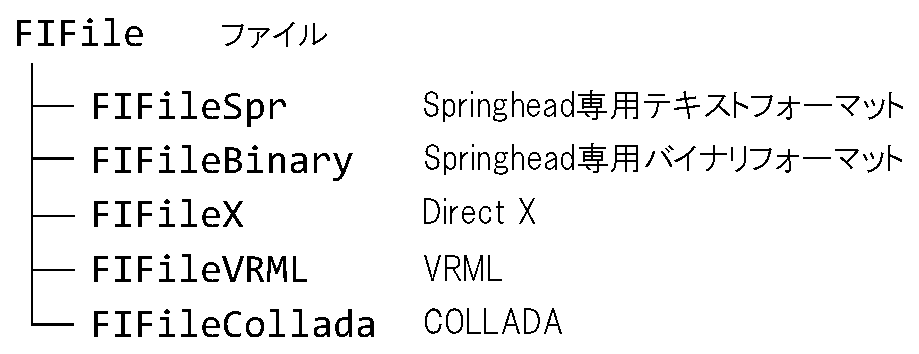
\includegraphics[width=.6\hsize]{fig/fifile.eps}
\end{center}
\caption{Class hierarchy of file objects}
\label{fig_fifile}
\end{figure}

\index{FIFile}
\index{�ӂ�����@�t�@�C��}
�t�@�C���I�u�W�F�N�g�́C�t�@�C������̃V�[���̃��[�h����уZ�[�u��S���܂��D
�t�@�C���̊��N���X��\texttt{FIFile}�ŁC�t�@�C���t�H�[�}�b�g�̎�ނ��Ƃɐ�p�̃t�@�C���N���X���h�����܂�
(\Fig{fifile})�D

�t�@�C���쐬�Ɋւ���\texttt{FISdk}�̊֐����ȉ��Ɏ����܂��D

\begin{center}
\begin{tabular}{p{.3\hsize}p{.6\hsize}}
\texttt{FISdkIf}															\\ \midrule
\texttt{FIFileSprIf*}		& \texttt{CreateFileSpr()}						\\
\texttt{FIFileBinaryIf*} 	& \texttt{CreateFileBinary()}					\\
\texttt{FIFileXIf*}			& \texttt{CreateFileX()}						\\
\texttt{FIFileVRMLIf*}		& \texttt{CreateFileVRML()}						\\
\texttt{FIFileCOLLADAIf*}	& \texttt{CreateFileCOLLADA()}					\\
\texttt{FIFileIf*}			& \texttt{CreateFileFromExt(UTString filename)}	\\
\end{tabular}
\end{center}

\texttt{CreateFileFromExt}��\texttt{filename}�̊g���q����t�@�C���t�H�[�}�b�g�𔻕ʂ��đΉ�����t�@�C���I�u�W�F�N�g���쐬���܂��D

\section{�t�@�C���t�H�[�}�b�g}
���̐߂ł�Springhead�Ń��[�h�E�Z�[�u�ł���t�@�C���̃t�@�C���t�H�[�}�b�g���Љ�܂��B

\subsection{spr�t�@�C��}
�g���q .spr �̃t�@�C���́ASpringhead�Ǝ��̃t�@�C���`���ł��B
�l���ǂݏ������₷���ASpringhead�̎d�l���ω����Ă��]��e�����󂯂Ȃ��悤�Ȍ`���ɂȂ��Ă��܂��B�t�@�C�����菑������ꍇ�͂��̌`�����g���Ă��������B

spr�t�@�C���̓m�[�h��`�̌J��Ԃ��ł��Bspr�t�@�C���̗�������܂��B

\begin{sourcecode}
PHSdk{                  #PHSdk�m�[�h
    CDSphere sphere{    #���̎q�m�[�h��CDSphere�m�[�h��lj�
        material = {    # CDSphere �� material(PHMaterial�^)��
            mu = 0.2    # ���C�W�� mu ��0.2����
        }
        radius = 0.5    # radius��0.5����
    }
    CDBox bigBox{
        boxsize = 2.0 1.1 0.9
    }
}
\end{sourcecode}

Spr�t�@�C���̃m�[�h�̓f�B�X�N���v�^�i\SECTION{if_desc})���Q�Ɓj�ɂP�΂P�őΉ����܂��B�f�B�X�N���v�^�����p�ӂ���Ύ����I�Ɏg����m�[�h�̌^�������܂��B
�t�@�C���Œl�������Ȃ��ƁA�f�B�X�N���v�^�̏����l�ɂȂ�܂��B
��̗�ł́A\texttt{PHSdk}�ɒlj������\texttt{sphere}(\texttt{CDSphere}�^)�́A
\begin{sourcecode}
CDSphereDesc desc;
desc.material.mu = 0.2;
desc.radius = 0.5;
\end{sourcecode}
�Ƃ����f�B�X�N���v�^ \texttt{desc} �ō��̂Ɠ������ƂɂȂ�܂��B

Spr�t�@�C���̕��@��BNF�{���K�\���ŏ�����
\begin{sourcecode}
spr   = node*
node  = node type, (node id)?, block
block = '{' (node|refer|data)*  '}'
refer = '*' node id
data  = field id, '=', (block | right)
right = '[' value*, ']' | value
value = bool | int | real | str | right
\end{sourcecode}
�ƂȂ�܂��B\texttt{right}�ȍ~�̉��߂�\texttt{field}�̌^�Ɉˑ����܂��B

\subsection{X�t�@�C��}
�u X �t�@�C�� �v�́ADirect3D�̃t�@�C���t�H�[�}�b�g�ŁA�g���q�� .x �ł��B
���f�����O�\�t�gXSI�Ŏg���Ă���A�����̃��f�����O�c�[���ŏo�͂ł��܂��B
3D�̌`��f�[�^�A�}�e���A���A�e�N�X�`���A�{�[���Ȃǂ��܂߂邱�Ƃ��ł��܂��B
Springhead2�ł́A�W���I��X�t�@�C���̃��[�h�ƁASpringhead2�Ǝ��̃m�[�h��
���[�h�ƃZ�[�u���ł��܂��B�������Ǝ��m�[�h���菑������ꍇ�� Spr�t�@�C��
�̕��������₷���֗��ł��̂ł�����̎g�p���������߂��܂��B

X�t�@�C���̗�������܂��B
\begin{sourcecode}
xof 0302txt 0064        #�ŏ��̍s�͂��ꂩ��n�܂�

#    �m�[�h�́C
#        �^���C�m�[�h�� { �t�B�[���h�̌J��Ԃ�   �q�m�[�h }
#    ����Ȃ�D
PHScene scene1{
    0.01;0;;            #�t�B�[���h �� �l; �̌J��Ԃ�
    1;0;-9.8;0;;        #�l�� ���l�C������܂��̓t�B�[���h
    PHSolid soFloor{    #�q�m�[�h�́C�m�[�h�Ɠ���
        (�ȗ�)
    }
}
# �R�����g�� #�ȊO�� // ���g����
\end{sourcecode}

\subsubsection{�Ǝ��m�[�h�̒�`}
Springhead2 �̒ʏ�̃m�[�h�́C�I�u�W�F�N�g�̃f�B�X�N���v�^�i\SECTION{if_desc}�߁j�ɂP�΂P�őΉ����܂��D
���[�h���ɂ́C�f�B�X�N���v�^�ɑΉ�����I�u�W�F�N�g����������C�V�[���O���t�ɒlj�����܂��D
�Z�[�u���ɂ́C�I�u�W�F�N�g����f�B�X�N���v�^��ǂݏo���C�m�[�h�̌`���Ńt�@�C���ɕۑ�����܂��D

�I�u�W�F�N�g�̃f�B�X�N���v�^�ɂ́C�K���Ή�����m�[�h������܂��D
�Ⴆ�΁C\texttt{SprPHScene.h} �ɂ́C

\begin{sourcecode}
struct PHSceneState{
    double timeStep;      ///< �ϕ��X�e�b�v
    unsigned count;       ///< �ϕ�������
};
struct PHSceneDesc:PHSceneState{
    /// �ڐG�E�S�������G���W���̎��
    enum ContactMode{ MODE_NONE, MODE_PENALTY, MODE_LCP};
    Vec3f gravity;      ///< �d�͉����x�x�N�g���D�f�t�H���g�l��(0.0f, -9.8f,0.0f)�D
};
\end{sourcecode}

�̂悤�ɁC�X�e�[�g�ƃf�B�X�N���v�^���錾����Ă��܂��D���� \texttt{PHSceneDesc} �ɑΉ����� X �t�@�C���̃m�[�h�́C
\begin{sourcecode}
PHScene scene1{                                                                     0.01;     #PHSceneState::timeStep
    0;;       #PHSceneState::count     �Ō��;��PHSceneState���̏I���������D
    1;        #PHSceneDesc::ContactMode
    0;-9.8;0;;#PHSceneDesc::gravity    �Ō��;��PHSceneDesc���̏I���������D
}
\end{sourcecode}

�̂悤�ɂȂ�܂��D�N���X�̃����o�ϐ������̂܂܃t�B�[���h�ɂȂ�܂��D
�܂��C��{�N���X�́C�擪�Ƀt�B�[���h���lj����ꂽ�`�ɂȂ�܂��D

�ʏ�m�[�h�̈ꗗ�� \URL{TBU: �f�X�N���v�^�ꗗ�̃y�[�W} ���Q�Ɖ������D

\subsubsection{X�t�@�C���̃m�[�h}
Springhead2�̓Ǝ��m�[�h�����łȂ��A���ʂ�X�t�@�C���̃m�[�h�����[�h�ł��܂��B
X�t�@�C���ɂ́A
\begin{sourcecode}
Frame{
    FrameTransfromMatrix{ 1,0,0,0, 0,1,0,0, 0,0,1,0, 0,0,0,1; }
}
\end{sourcecode}
�̂悤�ȃt���[���̃m�[�h�^������܂����A
Sprinhead2 �ɂ͑Ή�����f�B�X�N���v�^��I�u�W�F�N�g������܂���D
�����ŁC�����́A\texttt{GRFrame}��\texttt{PHFrame}��
�ϊ�����ă��[�h����܂��D
\URL{TBW �m�[�h�ꗗ�̃y�[�W(pageNodeDefList)} ���Q�Ɖ������D


\section{�t�@�C���̃��[�h�E�Z�[�u}
\begin{figure}
\begin{center}
\includegraphics*[width=.95\hsize]{fig/fileOperation.eps}
\end{center}
\caption{Overview of file operation}
\label{fig_fileOperation}
\end{figure}

\Fig{fileOperation}�́A�t�@�C���̃��[�h�E�Z�[�u�̎菇�������Ă��܂��B
���[�h���ɂ͂܂��t�@�C�����p�[�X���ăf�B�X�N���v�^�̃c���[�����܂��B
���Ƀf�B�X�N���v�^�̃c���[�����ǂ�Ȃ���A�I�u�W�F�N�g�̃c���[�����܂��B
����A�Z�[�u���ɂ́A�f�B�X�N���v�^�c���[�͍��܂���B
�I�u�W�F�N�g�c���[�����ǂ�Ȃ���I�u�W�F�N�g����f�B�X�N���v�^�����A���̏�Ńt�@�C���ɏ��������Ă����܂��B

�t�@�C���̃m�[�h�ƃf�B�X�N���v�^�c���[�̃m�[�h�͂P�΂P�ɑΉ����܂����A�I�u�W�F�N�g�̃c���[�ł͂����Ƃ͌���܂���B

\subsection{�t�@�C�����[�h�̎d�g��}
\subsubsection{�t�@�C���̃p�[�X}
�t�@�C���̃��[�h�́A\texttt{FIFileSpr}��\texttt{FIFileX}�̂悤��\texttt{FIFile}�̔h���N���X��\texttt{LoadImp()}���\�b�h���s���܂��B
�t�@�C���p�[�X�̎����́Aboost::spirit��p���Ď�������Ă��܂��B\texttt{Init()}���\�b�h�Ńp�[�T�̕��@���`���Ă��܂��B
\subsubsection{�f�B�X�N���v�^�̐���}
�p�[�T��\texttt{FILoadContext}���R���e�L�X�g�Ƃ��ėp���Ȃ���p�[�X��i�߂܂��B
\texttt{fieldIts}�Ƀ��[�h���̃f�[�^�̌^�����Z�b�g���Ă����܂��B
�m�[�h���⃁���o������f�B�X�N���v�^�⃁���o�̌^��m��K�v������܂����A�r���h����SWIG�Ő������Ă���f�B�X�N���v�^�̌^����\texttt{??Sdk::RegisterSdk()}���o�^�������̂�p���Ă��܂��B
�V�����m�[�h���o�Ă���x��\texttt{FILoadContext::datas}�Ƀf�B�X�N���v�^��p�ӂ��A�f�[�^�����[�h����Ƃ����ɒl���Z�b�g���Ă����܂��B
���̃m�[�h�ւ̎Q�Ƃ́A���̎��_�ł̓m�[�h���̕�����ŋL�^���Ă����܂��B
\subsubsection{�Q�Ƃ̃����N}
�t�@�C�������ׂă��[�h���I���ƁA\texttt{LoadImp()}���甲���āA\texttt{FIFile::Load(FILoadContext*)}�ɖ߂��Ă��܂��B
���̃m�[�h(���̃f�B�X�N���v�^)�ւ̎Q�Ƃ��m�[�h���̕�����𗊂�Ƀ|�C���^�ł‚Ȃ��ł����܂��B
\subsubsection{�I�u�W�F�N�g�̐���}
�I�u�W�F�N�g�����́A\texttt{FILoadContext::CreateScene()}���A
�f�B�X�N���v�^�c���[�����{���炽�ǂ�Ȃ��珇�ɍs���܂��B
�f�B�X�N���v�^����I�u�W�F�N�g�𐶐�����̂́A���̃I�u�W�F�N�g�̐�c�I�u�W�F�N�g�ł��B��c�I�u�W�F�N�g�������ł��Ȃ��ꍇ��SDK�̐��������݂܂��B
SDK�ȊO����ԍ��{�ɂ���t�@�C�������[�h���邽�߂ɂ́A�\�ߐ�c�I�u�W�F�N�g��p�ӂ��Ă����K�v������܂��B
\texttt{FIFile::Load(ObjectIfs\& objs, const char* fn)}��\texttt{objs}�����͂��̖��������܂��B

�������ꂽ�I�u�W�F�N�g�́A�e��\texttt{AddChildObject()}�ł����Ɏq�Ƃ��Ēlj�����܂��B

\subsubsection{�Q�Ƃ̃����N}
�f�B�X�N���v�^�Ԃ̎Q�Ƃ̓|�C���^�ɂȂ��Ă��܂����A�V�[���O���t�͌q�����Ă��܂���B�f�B�X�N���v�^�̎Q�Ƃɏ]���āA�f�B�X�N���v�^���琶�����ꂽ�I�u�W�F�N�g�ԂɎQ�Ƃ�lj����܂��B�����N�́A\texttt{AddChildObject()}�֐����Ăяo�����Ƃōs���܂��B�e�q�ƎQ�Ƃ̋�ʂ͂‚��Ȃ��Ȃ�܂��B����m�[�h�̉��Ɏq�m�[�h�������Ă��A�ʂ̂Ƃ���ɏ������m�[�h�ւ̎Q�Ƃ������Ă������V�[�O���t�ɂȂ�킯�ł��B

\subsection{�t�@�C�����[�h�̎���}
Framework���g���̂ƊȒP�ł��B
\begin{sourcecode}
virtual void FWMyApp::Init(int argc, char* argv[]){
    UTRef<ImportIf> import = GetSdk()->GetFISdk()->CreateImport();
    GetSdk()->LoadScene(fileName, import);  // �t�@�C���̃��[�h
    GetSdk()->SaveScene("save.spr", import);// �t�@�C���̃Z�[�u�e�X�g
\end{sourcecode}

FISdk�P�̂Ŏg���ꍇ�͎��̂悤�ɂȂ�܂��B
\begin{sourcecode}
int main(){
    //  �t�@�C�����[�_�Ő����ł���悤�ɁA�eSDK�̌^����o�^
    PHSdkIf::RegisterSdk();
    GRSdkIf::RegisterSdk();
    FWSdkIf::RegisterSdk();
    //  �t�@�C���̃��[�h
    UTRef<FISdkIf> fiSdk = FISdkIf::CreateSdk();
    FIFileIf* file = fiSdk->CreateFileFromExt(".spr");
    ObjectIfs objs; //  ���[�h�p�I�u�W�F�N�g�X�^�b�N
    fwSdk = FWSdkIf::CreateSdk();   //  FWSDK��p��
    //  �q�I�u�W�F�N�g�쐬�p��fwSdk���X�^�b�N�ɐς�
    objs.push_back(fwSdk);
    //  FWSDK�ȉ��S�̂��t�@�C�����烍�[�h
    if (! file->Load(objs, "test.spr") ) {  
        DSTR << "Error: Cannot open load file. " << std::endl;
        exit(-1);
    }
    //  �t�@�C�����̃��[�g�m�[�h�i�����̉”\������j��objs�ɐς܂��B
    for(unsigned  i=0; i<objs.size(); ++i){ 
        objs[i]->Print(DSTR);
    }
    ...
\end{sourcecode}

\subsection{�t�@�C���Z�[�u�̎d�g��}
�t�@�C���Z�[�u�́A\texttt{FIFile}���V�[���O���t�����ǂ�Ȃ���A�I�u�W�F�N�g���Z�[�u���Ă����܂��B
�e�I�u�W�F�N�g��
\texttt{GetDescAddress()}���A��������Ă��Ȃ����\texttt{GetDesc()}���Ăяo����
�f�B�X�N���v�^��ǂݏo���܂��B
�V�[���O���t�ɂ́A����m�[�h�������̃m�[�h�̎q�m�[�h�ɂȂ��Ă���ꍇ�����邽�߁A2�d�ɃZ�[�u���Ȃ��悤��2�x�ڈȍ~�͎Q�ƂƂ��ăZ�[�u���܂��B

�f�B�X�N���v�^�����o������A�f�B�X�N���v�^�̌^���𗘗p���āA�f�B�X�N���v�^�̃����o�����ԂɃZ�[�u���Ă����܂��B
���ۂɃf�[�^���t�@�C���ɕۑ�����R�[�h�́A\texttt{FiFileSpr}�Ȃ�\texttt{FiFile}�̔h���N���X�ɂ���܂��B

\subsection{�t�@�C���Z�[�u�̎���}
Framework���g���̂ƊȒP�ł��B
\begin{sourcecode}
virtual void FWMyApp::Save(const char* filename){
    UTRef<ImportIf> import = GetSdk()->GetFISdk()->CreateImport();
    GetSdk()->SaveScene(filename, import);	// filename�ɃV�[�����Z�[�u
\end{sourcecode}

FISdk�P�̂Ŏg���ꍇ�͎��̂悤�ɂȂ�܂��B
\begin{sourcecode}
void save(const char* filename, ImportIf* ex, ObjectIf* rootNode){
    //  �t�@�C���̃Z�[�u
    UTRef<FISdkIf> fiSdk = FISdkIf::CreateSdk();
    FIFileIf* file = fiSdk->CreateFileFromExt(".spr");
    ObjectIfs objs; //  ���[�h�p�I�u�W�F�N�g�X�^�b�N
    objs.push_back(rootNode);
    file->SetImport(ex);
    file->Save(*objs, filename);
}
\end{sourcecode}

\section{�C���|�[�g���̊Ǘ�}
T.B.W.
�iImport���g���ƕʂ̃t�@�C���ɏ������m�[�h���Ăяo�����Ƃ��ł���B
Import���g���ă��[�h�����V�[�����Z�[�u�ꍇ�A�t�@�C���ۑ����ɂǂ��܂ł�
�t�@�C���ɕۑ�����̂������ɂȂ�B
������Ǘ�����̂�Import�̖������Ǝv���Bby ���J��)
%\end{document}


\chapter{HumanInterface}
\label{chap_humaninterface}
\section{�T�v}

\index{HumanInterface}
HumanInterface���W���[���́C�n�[�h�E�F�A����̓f�o�C�X�𗘗p���邽�߂̏����n�Ɉˑ����Ȃ��C���^�t�F�[�X��񋟂��܂��D

�قƂ�ǂ̏ꍇ�CHumanInterface�̋@�\��Framework���W���[������ăA�N�Z�X���邱�ƂɂȂ�܂��D
���̏ꍇ�́C��q����q���[�}���C���^�t�F�[�X�I�u�W�F�N�g��f�o�C�X�̍쐬�����[�U���g�ōs���K�v�͂���܂���D

\section{HumanInterface SDK}

\index{HISdk}
HumanInterface���W���[���̂��ׂẴI�u�W�F�N�g��SDK�N���X\texttt{HISdk}�ɂ���ĊǗ�����܂��D
\texttt{HISdk}�N���X�́C�v���O�����̎��s��ʂ��Ă����P�‚̃I�u�W�F�N�g�����݂���V���O���g���N���X�ł��D
\texttt{HISdk}�I�u�W�F�N�g���쐬����ɂ͈ȉ��̂悤�ɂ��܂��D
\begin{sourcecode}
HISdkIf* hiSdk = HISdkIf::CreateSdk();
\end{sourcecode}
�ʏ킱�̑���̓v���O�����̏��������Ɉ�x�������s���܂��D
�܂��CFramework���W���[�����g�p����ꍇ�̓��[�U������\texttt{HISdk}���쐬����K�v�͂���܂���D

\section{�N���X�K�w�ƃf�[�^�\��}

\begin{figure}[t]
\begin{center}
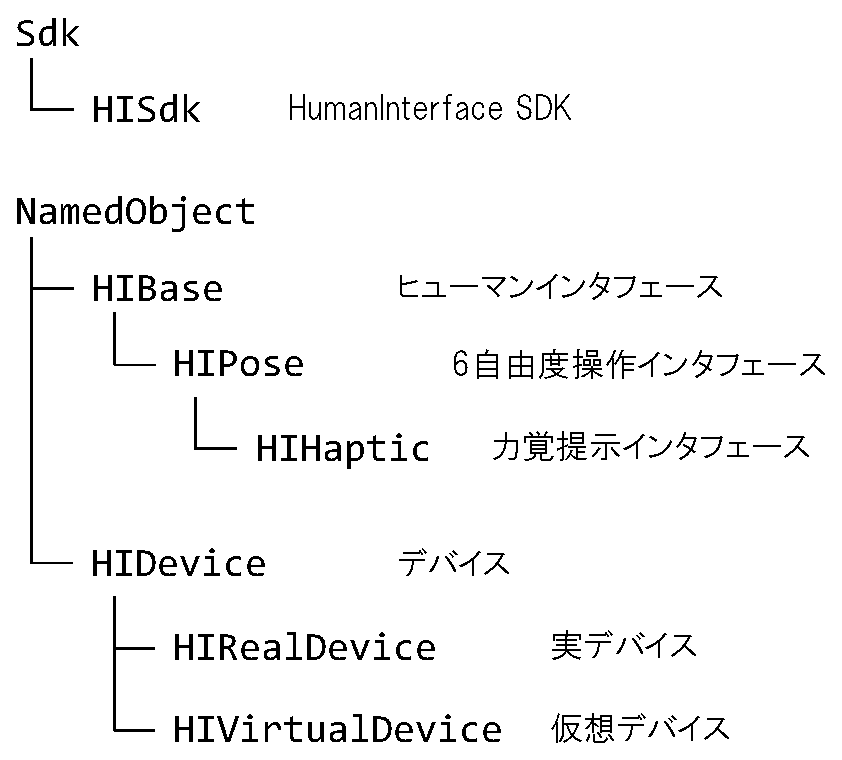
\includegraphics[width=.5\hsize]{fig/hiclass.eps}
\end{center}
\caption{HumanInterface class hierarchy}
\label{fig_hiclass}
\end{figure}

HumanInterface���W���[���̃N���X�K�w��Fig.\,\ref{fig_hiclass}�Ɏ����܂��D

�f�o�C�X�ɂ͎��f�o�C�X�Ɖ��z�f�o�C�X������܂��D
���f�o�C�X�͌����̃n�[�h�E�F�A�ɑΉ����C�Ⴆ��Win32�}�E�X�₠�郁�[�J��A/D�ϊ��{�[�h��\�����f�o�C�X������܂��D
����C���z�f�o�C�X�͎��f�o�C�X���񋟂���@�\�P�ʂ�\���C�����n�Ɉˑ����܂���D
�Ⴆ�΁C1�‚�A/D�ϊ��|�[�g�⒊�ۉ����ꂽ�}�E�X�C���^�t�F�[�X������ɂ�����܂��D
��{�I�ɁC���������������Ă̓��[�U�͎��f�o�C�X�ɐG��邱�Ƃ͂Ȃ��C���z�f�o�C�X��ʂ��Ă����̋@�\�𗘗p���邱�ƂɂȂ�܂��D

�q���[�}���C���^�t�F�[�X�̓f�o�C�X�������x�Œ��ۉ����ꂽ����C���^�t�F�[�X��񋟂��܂��D


\begin{figure}[t]
\begin{center}
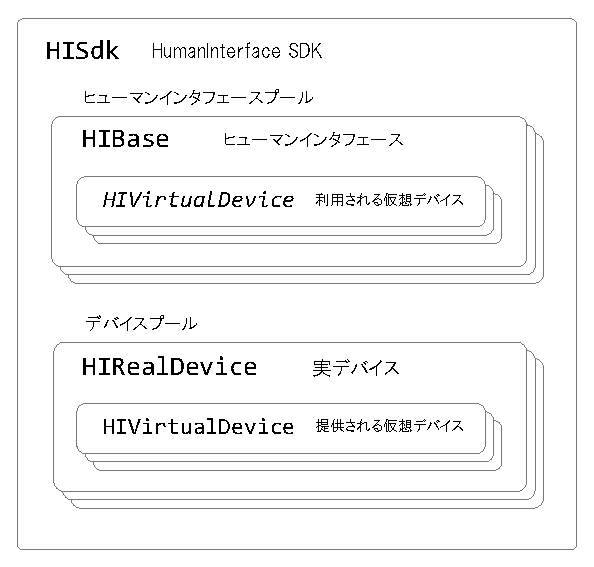
\includegraphics[width=.5\hsize]{fig/humaninterface.eps}
\end{center}
\caption{HumanInterface module data structure}
\label{fig_humaninterface}
\end{figure}

����HumanInterface���W���[���̃f�[�^�\����Fig.\,\ref{fig_humaninterface}�Ɏ����܂��D
\texttt{HISdk}�I�u�W�F�N�g�̓q���[�}���C���^�t�F�[�X�v�[���ƃf�o�C�X�v�[���������Ă��܂��D
�f�o�C�X�v�[���Ƃ͎��f�o�C�X�̏W�܂�ŁC���ꂼ��̎��f�o�C�X�͂��̋@�\�������‚��̉��z�f�o�C�X�Ƃ��ĊO���ɒ񋟂��܂��D

�f�o�C�X�̋@�\���g���ɂ́C
\begin{enumerate}
\item ���f�o�C�X���쐬����
\item ���f�o�C�X���񋟂��鉼�z�f�o�C�X�ɃA�N�Z�X����
\end{enumerate}
�Ƃ���2�i�K�̎菇�𓥂݂܂��D
�ȉ��ɂ���Ɋ֌W����\texttt{HISdk}�̊֐����Љ�܂��D
\begin{center}
\begin{tabular}{p{.25\hsize}p{.65\hsize}}
\texttt{HISdkIf}																		\\ \midrule
\texttt{HIRealDeviceIf*}	& \texttt{AddRealDevice(const IfInfo* ii, const void* desc = NULL)} \\
\texttt{HIRealDeviceIf*}	& \texttt{FindRealDevice(const char* name)} \\
\texttt{HIRealDeviceIf*}	& \texttt{FindRealDevice(const IfInfo* ii)}
\end{tabular}
\end{center}
\texttt{AddRealDevice}�͌^���\texttt{ii}�ƃf�B�X�N���v�^\texttt{desc}���w�肵�Ď��f�o�C�X���쐬���܂��D
\texttt{FindRealDevice}�͖��O���^�����w�肵�āC�����̎��f�o�C�X���������܂��D
���Ƃ��΁C������GLUT��p����L�[�{�[�h�E�}�E�X���f�o�C�X���擾����ɂ�
\begin{sourcecode}
hiSdk->FindRealDevice(DRKeyMouseGLUTIf::GetIfInfoStatic());
\end{sourcecode}
�Ƃ��܂��D

���z�f�o�C�X���擾����ѕԋp������@�ɂ�\texttt{HISdk}�������@��\texttt{HIRealDevice}�𒼐ڌĂяo�����@��2�ʂ肪����܂��D
\begin{center}
\begin{tabular}{p{.25\hsize}p{.65\hsize}}
\texttt{HISdkIf}																							\\ \midrule
\texttt{HIVirtualDeviceIf*} & \texttt{RentVirtualDevice(const IfInfo* ii, const char* name, int portNo)}	\\
\texttt{bool}				& \texttt{ReturnVirtualDevice(HIVirtualDeviceIf* dev)}	\\
\end{tabular}
\end{center}
\texttt{RentVirtualDevice}�̓f�o�C�X�v�[�����X�L�������Č^���ɍ��v�����ŏ��̉��z�f�o�C�X��Ԃ��܂��D
���f�o�C�X�����肵�����ꍇ��\texttt{name}�Ŏ��f�o�C�X�����w�肵�܂��D
�܂��C�����̉��z�f�o�C�X��񋟂�����f�o�C�X������܂��D
���̏ꍇ�̓|�[�g�ԍ�\texttt{portNo}�Ŏ擾���������z�f�o�C�X���w��ł��܂��D
%
�f�o�C�X�̋�����h�����߂ɁC��x�擾���ꂽ���z�f�o�C�X�͗��p����ԂɂȂ�܂��D
���p���̃f�o�C�X�͐V���Ɏ擾���邱�Ƃ͂ł��܂���D
�g���I������f�o�C�X��\texttt{ReturnVirtualDevice}�ŕԋp���邱�Ƃɂ���čĂю擾�”\�ɂȂ�܂��D
\begin{center}
\begin{tabular}{p{.25\hsize}p{.65\hsize}}
\texttt{HIRealDeviceIf}																				\\ \midrule
\texttt{HIVirtualDeviceIf*}	& \texttt{Rent(const IfInfo* ii, const char* name, int portNo)}	\\
\texttt{bool}				& \texttt{Return(HIVirtualDeviceIf* dev)}
\end{tabular}
\end{center}
������͎��f�o�C�X���璼�ڎ擾�C�ԋp���邽�߂̊֐��ł��D�@�\�͓��l�ł��D


\section{���f�o�C�X}

Springhead�ł͂����‚��̃��[�J���̃n�[�h�E�F�A�����f�o�C�X�Ƃ��ăT�|�[�g����Ă��܂����C
�����n�ɋ����ˑ����镔���ł��邽�ߖ{�h�L�������g�̑ΏۊO�Ƃ��܂��D
�����̂�����̓\�[�X�R�[�h�����Ă��������D

\section{�L�[�{�[�h�E�}�E�X}
\label{sec_hi_keymouse}

�L�[�{�[�h����у}�E�X�̋@�\�͕����1�‚̃N���X�Ƃ��Ē񋟂���Ă��܂��D
�L�[�{�[�h�E�}�E�X�̉��z�f�o�C�X��\texttt{DVKeyMouse}�ł��D
���f�o�C�X�Ƃ��Ă�Win32 API��p����\texttt{DRKeyMouseWin32}��GLUT��p����\texttt{DRKeyMouseGLUT}������܂��D
�񋟂����@�\�ɑ����̍��ق�����̂Œ��ӂ��ĉ������D

\subsection*{���z�L�[�R�[�h}

Ascii�O�̓���L�[�ɂ͏����n�ˑ��̃L�[�R�[�h�����蓖�Ă��Ă��܂��D
���̍����z�����邽�߂Ɉȉ��̃V���{����\texttt{DVKeyCode}�񋓌^�Œ�`����Ă��܂��D

\begin{center}
\begin{tabular}{p{.3\hsize}p{.6\hsize}}
\texttt{DVKeyCode}									\\ \midrule
\texttt{ESC}				& �G�X�P�[�v			\\
\texttt{F1} - \texttt{F12}	& �t�@���N�V�����L�[	\\
\texttt{LEFT}				& ��					\\
\texttt{UP}					& ��					\\
\texttt{RIGHT}				& ��					\\
\texttt{DOWN}				& ��					\\
\texttt{PAGE\_UP}			& Page Up				\\
\texttt{PAGE\_DOWN}			& Page Down				\\
\texttt{HOME}				& Home					\\
\texttt{END}				& End					\\
\texttt{INSERT}				& Insert				\\
\end{tabular}
\end{center}

�K�v�ɉ����ăV���{�����lj������”\��������܂��̂ŁC���S�ȃ��X�g�̓w�b�_�t�@�C���Ŋm�F���Ă��������D

\subsection*{�R�[���o�b�N}

\texttt{DVKeyMouse}����̃C�x���g����������ɂ�\texttt{DVKeyMouseCallback}�N���X���p�����C�C�x���g�n���h�����I�[�o���C�h���܂��D
\texttt{DVKeyMouseCallback}�͂����‚��̃q���[�}���C���^�t�F�[�X�N���X���p�����Ă���ق��C
��q����A�v���P�[�V�����N���X\texttt{FWApp}���p�����Ă��܂��D

\begin{center}
\begin{tabular}{p{.2\hsize}p{.7\hsize}}
\texttt{DVKeyMouseCallback}								\\ \midrule
\texttt{virtual bool} & \texttt{OnMouse(int button, int state, int x, int y)}		\\
\multicolumn{2}{l}{�}�E�X�{�^���v�b�V��/�����[�X}	\\
\\
\texttt{virtual bool} & \texttt{OnDoubleClick(int button, int x, int y)}			\\
\multicolumn{2}{l}{�_�u���N���b�N}	\\
\\
\texttt{virtual bool} & \texttt{OnMouseMove(int button, int x, int y, int zdelta)}	\\
\multicolumn{2}{l}{�}�E�X�J�[�\���ړ�/�}�E�X�z�C�[����]}	\\
\\
\texttt{virtual bool} & \texttt{OnKey(int state, int key, int x, int y)}			\\
\multicolumn{2}{l}{�L�[�v�b�V��/�����[�X}	\\
\end{tabular}
\end{center}

\texttt{OnMouse}�̓}�E�X�{�^���̃v�b�V�����邢�̓����[�X���������Ƃ��ɌĂяo����܂��D
\texttt{button}�̓C�x���g�Ɋ֌W����}�E�X�{�^������т����‚��̓���L�[�̎��ʎq��ێ����C
���̒l��\texttt{DVButtonMask}�񋓎q�̒l��OR�����ŕ\������܂��D
\texttt{state}�̓}�E�X�{�^����ԕω��������C\texttt{DVButtonSt}�񋓎q�̂����ꂩ�̒l�������܂��D
\texttt{x}�C\texttt{y}�̓C�x���g�������̃J�[�\�����W��\���܂��D
��Ƃ��āC���{�^���̃v�b�V���C�x���g����������ɂ͎��̂悤�ɂ��܂��D
\begin{sourcecode}
// inside your class definition ...
virtual bool OnMouse(int button, int state, int x, int y){
    if(button & DVButtonMask::LBUTTON && state == DVButtonSt::DOWN){
        // do something here
    }
}
\end{sourcecode}

\texttt{OnDoubleClick}�̓}�E�X�{�^���̃_�u���N���b�N���������Ƃ��ɌĂ΂�܂��D
�����̒�`��\texttt{OnMouse}�Ɠ��l�ł��D

\texttt{OnMouseMove}�̓}�E�X�J�[�\�����ړ����邩�C�}�E�X�z�C�[������]�����ۂɌĂ΂�܂��D
\texttt{button}�͒��O�̃}�E�X�v�b�V���C�x���g�ɂ�����\texttt{OnMouse}�ɓn���ꂽ�̂Ɠ����l�������܂��D
\texttt{x}, \texttt{y}�͈ړ���̃J�[�\�����W�C\texttt{zdelta}�̓}�E�X�J�[�\���̉�]�ʂł��D

\texttt{OnKey}�̓L�[�{�[�h�̃L�[���v�b�V������邩�����[�X���ꂽ�ۂɌĂ΂�܂��D
\texttt{state}��\texttt{DVKeySt}�񋓎q�̒l�������܂��D
\texttt{key}�̓v�b�V�����邢�̓����[�X���ꂽ�L�[�̉��z�L�[�R�[�h��ێ����܂��D

�ȉ��Ɋ֘A����񋓎q�̒�`�������܂��D

\begin{center}
\begin{tabular}{p{.3\hsize}p{.6\hsize}}
\texttt{DVButtonMask}									\\ \midrule
\texttt{LBUTTON}				& ���{�^��				\\
\texttt{RBUTTON}				& �E�{�^��				\\
\texttt{MBUTTON}				& ���{�^��				\\
\texttt{SHIFT}					& Shift�L�[��������		\\
\texttt{CONTROL}				& Ctrl�L�[��������		\\
\texttt{ALT}					& Alt�L�[��������		\\
\end{tabular}
\end{center}

\begin{center}
\begin{tabular}{p{.3\hsize}p{.6\hsize}}
\texttt{DVButtonSt}								\\ \midrule
\texttt{DOWN}			& �{�^���v�b�V��		\\
\texttt{UP}				& �{�^�������[�X		\\
\end{tabular}
\end{center}

\begin{center}
\begin{tabular}{p{.3\hsize}p{.6\hsize}}
\texttt{DVKeySt}								\\ \midrule
\texttt{PRESSED}		& ���������			\\
\texttt{TOGGLE\_ON}		& �g�O���������		\\
\end{tabular}
\end{center}

\subsection*{API�Ƃ��Ē񋟂����@�\}

�ȉ���\texttt{DVKeyMouse}�̊֐��������܂��D
\begin{center}
\begin{tabular}{p{.1\hsize}p{.8\hsize}}
\texttt{DVKeyMouseIf}																		\\ \midrule
\texttt{void}	& \texttt{AddCallback(DVKeyMouseCallback*)} 	\\
\texttt{void}	& \texttt{RemoveCallback(DVKeyMouseCallback*)} 	\\
\texttt{int}	& \texttt{GetKeyState(int key)}					\\
\texttt{void}	& \texttt{GetMousePosition(int\& x, int\& y, int\& time, int count=0)}
\end{tabular}
\end{center}
\texttt{AddCallback}�̓R�[���o�b�N�N���X��o�^���܂��D
��‚̉��z�f�o�C�X�ɑ΂��ĕ����‚̃R�[���o�b�N��o�^�ł��܂��D
\texttt{RemoveCallback}�͓o�^�ς̃R�[���o�b�N�N���X���������܂��D

\texttt{GetKeyState}��\texttt{DVKeyCode}�Ŏw�肵���L�[�̏�Ԃ�\texttt{DVKeySt}�̒l�ŕԂ��܂��D

\texttt{GetMousePosition}��\texttt{count}�X�e�b�v�O�̃}�E�X�J�[�\���̈ʒu���擾����̂ɗp���܂��D
������\texttt{count}��$0$�ȏ�$63$�ȉ��łȂ���΂Ȃ�܂���D
\texttt{x}, \texttt{y}�ɃJ�[�\�����W���C\texttt{time}�Ƀ^�C���X�^���v���i�[����܂��D

\subsection*{�T�|�[�g�󋵂Ɋւ��钍��}

�g�p������f�o�C�X�ɂ���Ă͈ꕔ�̋@�\���񋟂���Ȃ��̂Œ��ӂ��ĉ������D

\texttt{OnMouseMove}�ɂ����ă}�E�X�z�C�[���̉�]�ʂ��擾����ɂ́C
���f�o�C�X�Ƃ���\texttt{DRKeyMouseWin32}���g�p���邩�C
freeglut�ƃ����N���ăr���h����Springhead���\texttt{DRKeyMouseGLUT}���g�p����K�v������܂��D

\texttt{OnKey}�ɂ����ăL�[�̃g�O����Ԃ��擾����ɂ�
���f�o�C�X�Ƃ���\texttt{DRKeyMouseWin32}���g�p����K�v������܂��D

\texttt{GetKeyState}��\texttt{DRKeyMouseWin32}�ł̂݃T�|�[�g����܂��D

\texttt{GetMousePosition}�ɂ����āC�^�C���X�^���v���擾����ɂ�\texttt{DRKeyMouseWin32}��p����K�v������܂��D

\section{�W���C�X�e�B�b�N}

�W���C�X�e�B�b�N�̉��z�f�o�C�X��\texttt{DVJoyStick}�ł��D
���f�o�C�X�Ƃ��Ă�GLUT��p����\texttt{DRJoyStickGLUT}�݂̂�����܂��D

T.B.D. 

\section{�g���b�N�{�[��}

\begin{figure}[t]
\begin{center}
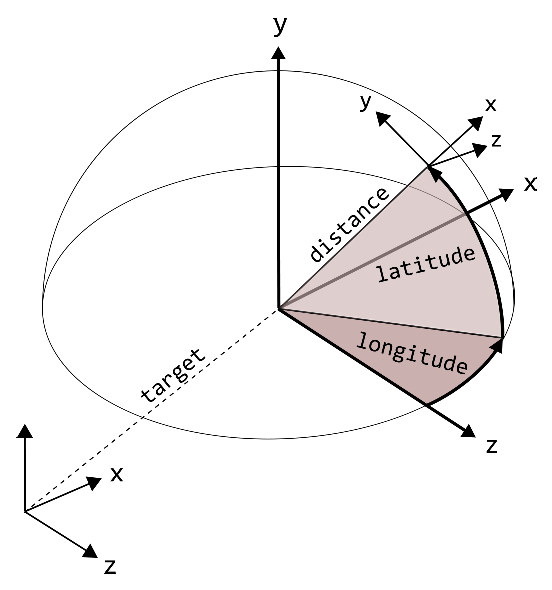
\includegraphics[width=.5\hsize]{fig/hitrackball.eps}
\end{center}
\caption{Trackball}
\label{fig_trackball}
\end{figure}

�g���b�N�{�[���̓L�[�{�[�h�E�}�E�X�ɂ����i�E��]��6���R�x����͂���q���[�}���C���^�t�F�[�X�ł��D
�g���b�N�{�[�����g�����Ƃɂ��C�J�����𒍎��_�܂��Ɏ��_�ύX���邱�Ƃ��ł���悤�ɂȂ�܂��D

�g���b�N�{�[���𑀍삷����@�ɂ́CAPI�𒼐ڌĂяo�����@�ƁC���z�}�E�X�ɃR�[���o�b�N�o�^������@�̓�ʂ肪����܂��D
���l�ɁC�g���b�N�{�[���̏�Ԃ��擾������@�ɂ�API�Ăяo���ƃR�[���o�b�N�o�^�̓�ʂ肪����܂��D
���z�}�E�X�ƃg���b�N�{�[������у��[�U�v���O�����̊֌W��\figurename\ref{fig_trackball}�Ɏ����܂��D


\subsection*{��]���S�Ɖ�]�p�x}

�J�����̈ʒu�ƌ����́C�����_�C�o�x�p�C�ܓx�p����ђ����_����̋����ɂ���Č��܂�܂��D

\begin{center}
\begin{tabular}{p{.15\hsize}p{.5\hsize}p{.25\hsize}}
\multicolumn{3}{l}{\texttt{HITrackballDesc}}				\\ \midrule
\texttt{Vec3f}	&	\texttt{target}			& ��]���S		\\
\texttt{float}	&	\texttt{longitude}		& �o�x[rad]		\\
\texttt{float}	&	\texttt{latitude}		& �ܓx[rad]		\\
\texttt{float}	&	\texttt{distance}		& ����			\\
\end{tabular}
\end{center}

\begin{center}
\begin{tabular}{p{.15\hsize}p{.75\hsize}}
\multicolumn{2}{l}{\texttt{HITrackballIf}}									\\ \midrule
\texttt{Vec3f}	& \texttt{GetTarget()}							\\
\texttt{void} 	& \texttt{SetTarget(Vec3f)}						\\
\texttt{void} 	& \texttt{GetAngle(float\& lon, float\& lat)}	\\
\texttt{void} 	& \texttt{SetAngle(float lon, float lat)}		\\
\texttt{float} 	& \texttt{GetDistance()}						\\
\texttt{void} 	& \texttt{SetDistance(float dist)}				\\
\end{tabular}
\end{center}

\subsection*{�͈͎w��}

�ȉ��̋@�\�Ŋp�x����ы����ɔ͈͐������������܂��D

\begin{center}
\begin{tabular}{p{.15\hsize}p{.5\hsize}p{.25\hsize}}
\multicolumn{3}{l}{\texttt{HITrackballDesc}}					\\ \midrule
\texttt{Vec2f}	&	\texttt{lonRange}		& �o�x�͈�			\\
\texttt{Vec2f}	&	\texttt{latRange}		& �ܓx�͈�			\\
\texttt{Vec2f}	&	\texttt{distRange}		& �����͈�			\\
\end{tabular}
\end{center}

\begin{center}
\begin{tabular}{p{.15\hsize}p{.75\hsize}}
\multicolumn{2}{l}{\texttt{HITrackballIf}}									\\ \midrule
\texttt{void} 	& \texttt{GetLongitudeRange(float\& rmin, float\& rmax)}	\\
\texttt{void} 	& \texttt{SetLongitudeRange(float rmin, float rmax)}		\\
\texttt{void} 	& \texttt{GetLatitudeRange(float\& rmin, float\& rmax)}		\\
\texttt{void} 	& \texttt{SetLatitudeRange(float rmin, float rmax)}			\\
\texttt{void} 	& \texttt{GetDistanceRange(float\& rmin, float\& rmax)}		\\
\texttt{void} 	& \texttt{SetDistanceRange(float rmin, float rmax)}			\\
\end{tabular}
\end{center}

\subsection*{�R�[���o�b�N�o�^}

\begin{center}
\begin{tabular}{p{.2\hsize}p{.7\hsize}}
\multicolumn{2}{l}{\texttt{HITrackballIf}}								\\ \midrule
\texttt{DVKeyMouseIf*} 	& \texttt{GetKeyMouse()}						\\
\texttt{void} 			& \texttt{SetKeyMouse(DVKeyMouseIf*)}			\\
\texttt{void} 			& \texttt{SetCallback(HITrackballCallback*)}	\\
\end{tabular}
\end{center}

�g���b�N�{�[�����}�E�X���삷��ɂ�\texttt{DVKeyMouse}�N���X�ɃR�[���o�b�N�o�^����K�v������܂��D
�R�[���o�b�N�o�^����ɂ�\texttt{SetKeyMouse}�C�o�^��̉��z�}�E�X���擾����ɂ�\texttt{GetKeyMouse}���Ăт܂��D

�܂��C���[�U�v���O�������g���b�N�{�[���ɃR�[���o�b�N�o�^���ď�ԕω��ɔ����ł���悤�ɂ���ɂ́C
\texttt{HITrackballCallback}�N���X���p�����C\texttt{SetCallback}�֐��ɓn���܂��D
\texttt{HITrackballCallback}�͈ȉ��̒P��̉��z�֐��������܂��D
\begin{center}
\begin{tabular}{p{.2\hsize}p{.7\hsize}}
\multicolumn{2}{l}{\texttt{HITrackballCallback}}					\\ \midrule
\texttt{virtual void} 	& \texttt{OnUpdatePose(HITrackballIf* tb)}	\\
\end{tabular}
\end{center}
\texttt{OnUpdatePose}�̓g���b�N�{�[���̈ʒu�E�����ɕω���������x�ɌĂ΂�܂��D
������\texttt{tb}�͌Ăяo�����̃g���b�N�{�[���������܂��D

\subsection*{�}�E�X�{�^��������}

\texttt{HITrackball}�͓�����\texttt{DVKeyMouseCallback}���p�����܂��D
\texttt{SetKeyMouse}�ɂ��\texttt{DVKeyMouse}�ɃR�[���o�b�N�o�^����ƁC
�}�E�X�J�[�\�����ړ����邽�т�\texttt{OnMouseMove}�C�x���g�n���h�����Ăяo����C�g���b�N�{�[���̓�����Ԃ��X�V����܂��D
�}�E�X�ړ����̃{�^����Ԃɉ����ăg���b�N�{�[���̂ǂ̏�Ԃ��ω����邩�͂�����x�J�X�^�}�C�Y���”\�ł��D
�ȉ��Ɋ֘A����@�\�������܂��D

\begin{center}
\begin{tabular}{p{.15\hsize}p{.35\hsize}p{.4\hsize}}
\multicolumn{3}{l}{\texttt{HITrackballDesc}}		\\ \midrule
\texttt{int}	& \texttt{rotMask}		& ��]����̃{�^��������		\\
\texttt{int}	& \texttt{zoomMask}		& �Y�[������̃{�^��������		\\
\texttt{int}	& \texttt{trnMask}		& ���s�ړ�����̃{�^��������	\\
\end{tabular}
\end{center}

\begin{center}
\begin{tabular}{p{.15\hsize}p{.75\hsize}}
\multicolumn{2}{l}{\texttt{HITrackballIf}}			\\ \midrule
\texttt{void} 	& \texttt{SetRotMask(int mask)}		\\
\texttt{void} 	& \texttt{SetZoomMask(int mask)}	\\
\texttt{void} 	& \texttt{SetTrnMask(int mask)}		\\
\end{tabular}
\end{center}

\texttt{rotMask}, \texttt{zoomMask}, \texttt{trnMask}�͂��ꂼ��
��]����C�Y�[������C���s�ړ�����Ɋ��蓖�Ă����}�E�X�{�^���ɑΉ�����
\texttt{OnMouseMove}��\texttt{button}�����̒l��\���܂��D
�ȉ��ɑΉ��֌W���܂Ƃ߂܂��D
\begin{center}
\begin{tabular}{p{.3\hsize}p{.3\hsize}p{.3\hsize}}
\toprule
�}�E�X�ړ�����		& \texttt{button}�l		& �ω���		\\ \midrule
���E				& \texttt{rotMask}		& �o�x			\\
�㉺				& \texttt{rotMask}		& �ܓx			\\
�㉺				& \texttt{zoomMask}		& ����			\\
���E				& \texttt{trnMask}		& �����_x���W	\\
�㉺				& \texttt{trnMask}		& �����_y���W	\\
\bottomrule
\end{tabular}
\end{center}
�f�t�H���g�̃{�^�������Ă͈ȉ��̒ʂ�ł��D
\begin{center}
\begin{tabular}{p{.3\hsize}p{.6\hsize}}
\texttt{rotMask}	& \texttt{LBUTTON}					\\
\texttt{zoomMask}	& \texttt{RBUTTON}					\\
\texttt{trnMask}	& \texttt{LBUTTON} + \texttt{ALT}	\\
\end{tabular}
\end{center}
���������āC���{�^���h���b�O�ʼn�]����C�E�{�^���h���b�O�ŃY�[������C[ALT]�L�[+���h���b�O�ŕ��s�ړ��ƂȂ�܂��D

�Ȃ��C����ł̓}�E�X�̈ړ������Ƃ̑Ή����J�X�^�}�C�Y���邱�Ƃ͂ł��܂���D
�܂��C�}�E�X�z�C�[���̉�]�ƃg���b�N�{�[����A��������@�\���������ł��D

\subsection*{�}�E�X����ɑ΂���ɐ��Ɗ��x}

�}�E�X�ړ��ʂƊp�x�ω��ʁC�����ω��ʂƂ̔��W�������L�̋@�\�Őݒ�ł��܂��D

\begin{center}
\begin{tabular}{p{.15\hsize}p{.35\hsize}p{.4\hsize}}
\multicolumn{3}{l}{\texttt{HITrackballDesc}}							\\ \midrule
\texttt{float}	&	\texttt{rotGain}		& ��]�Q�C��[rad/pixel]		\\
\texttt{float}	&	\texttt{zoomGain}		& �Y�[���Q�C��[rad/pixel]	\\
\texttt{float}	&	\texttt{trnGain}		& ���s�ړ��Q�C��			\\
\end{tabular}
\end{center}

\begin{center}
\begin{tabular}{p{.15\hsize}p{.75\hsize}}
\multicolumn{2}{l}{\texttt{HITrackballIf}}									\\ \midrule
\texttt{float} 	& \texttt{GetRotGain()}			\\
\texttt{void} 	& \texttt{SetRotGain(float g)}	\\
\texttt{float} 	& \texttt{GetZoomGain()}		\\
\texttt{void} 	& \texttt{SetZoomGain(float g)}	\\
\texttt{float} 	& \texttt{GetTrnGain()}			\\
\texttt{void} 	& \texttt{SetTrnGain(float g)}	\\
\end{tabular}
\end{center}

\subsection*{�g���b�N�{�[���Ŏ��_�𓮂���}

�g���b�N�{�[���̈ʒu�ƌ������J�����ɔ��f����ɂ́C
�`�揈���̖`���ňȉ��̂悤�ɂ��܂��D

\begin{sourcecode}
// given GRRenderIf* render
render->SetViewMatrix(trackball->GetAffine().inv());
\end{sourcecode}

\section{Spidar}

Spidar�̓��C���쓮�^��3���E6���͊o�񎦃q���[�}���C���^�t�F�[�X�ł��D

T.B.D. 




\chapter{Creature}
\label{chap_creature}
\begin{chapterabstract}
Creature���W���[���́C�����V�~�����[�^��p���ăo�[�`�����N���[�`���i�������삷��L�����N�^�j���쐬����@�\��񋟂��܂��D

Springhead�̕����V�~�����[�V�����@�\�́C�l�ԁE�����E�L�����N�^�E���{�b�g���̐g�̓�����V�~�����[�V�������邱�Ƃɂ����Ă����p���l������܂��D
���́E�֐ߌn�Őg�̃��f�����쐬���C�֐߂ɑg�ݍ��܂ꂽ����@�\��֐ߌn��IK�@�\��p���Đg�̓���𐶐����邱�Ƃ��ł��܂��D
�����V�~�����[�^���̏��i���̂̉^���E�`��E�ڐG�͓��j�𗘗p���ăo�[�`�����Ȋ��o�i�Z���T�j���̐������ł��܂��D���o�E����̃��[�v���񂷂��ƂŎ������삷��L�����N�^�⃍�{�b�g�������ł��܂��D

���������o�[�`�����ȃL�����N�^�E���{�b�g���𑍏̂��āC�o�[�`�����N���[�`���iCreature : �������j�ƌĂт܂��D
\end{chapterabstract}

% ----- ----- ----- ----- ----- ----- ----- ----- ----- ----- ----- ----- ----- ----- ----- ----- ----- ----- ----- -----
%
% ���h�L�������g�̏�������

% �@�\ ::= "�T��" �� �ڍ� ���t�@�����X*
% ��   ::= ["�R�[�h��" "�R�[�h��̐���"]*
% �ڍ� ::= [�@�\]*

% ���t�@�����X ::= [�f�B�X�N���v�^ | �C���^�t�F�[�X]

% - �����Ƃ��ă��t�@�����X�͋@�\�̂܂Ƃ߂ƕ��ɂƂǂ߂�D
% - Getter/Setter�͑Ή�����f�B�X�N���v�^�̃��t�@�����X�ɏ����C�C���^�t�F�[�X�̃��t�@�����X�ɂ͍ڂ��Ȃ��D
% - �}�� "�T��" "�R�[�h��" "�R�[�h��̐���" �œK�X�p����D������ "�R�[�h��" �̐}�͌����Ƃ��Ă��̃R�[�h�̎��s���ʂƂ���D

%
% ----- ----- ----- ----- ----- ----- ----- ----- ----- ----- ----- ----- ----- ----- ----- ----- ----- ----- ----- -----


% ----- ----- ----- ----- ----- ----- ----- ----- ----- ----- ----- ----- ----- ----- ----- ----- ----- -----
%
% �T��
% 

\section{Creature���W���[���̍\��}

���}��Creature���W���[���̃V�[���c���[�\���������܂��B

\begin{sourcecode}
CRSdk
+-- CRCreature
|   +-- CRBody
|   |   +-- CRBone
|   +-- CREngine (CRSensor, CRController)
\end{sourcecode}

\texttt{CRSdk}��Creature�̋@�\���g�p���鍪�{�ƂȂ�I�u�W�F�N�g�ł��B
\begin{sourcecode}
CRSdkIf* crSdk = CRSdkIf::CreateSdk();
\end{sourcecode}

\texttt{CRCreature}�́C�o�[�`�����N���[�`��$1$�̕��̋@�\�𓝊�����I�u�W�F�N�g�ł��D�g�́A���o��A������L���Ă��܂��DCRCreatureDesc�ɂ͓��ɐݒ肷�ׂ����ڂ͂���܂���B
\begin{sourcecode}
CRCreatureIf* crCreature = crSdk->CreateCreature(
  CDCreatureIf::GetIfInfoStatic(), CRCreatureDesc());
\end{sourcecode}
CRCreature���쐬������A�����V�~�����[�V�����̃V�[���Ɗ֘A�Â��邽�߂ɁAPHScene���q�I�u�W�F�N�g�Ƃ��ăZ�b�g���Ă��������B
\begin{sourcecode}
// PHSceneIf* phScene;   // should be taken from somewhere
crCreature->AddChildObject(phScene);
\end{sourcecode}

�V�~�����[�V�������s���́A1�X�e�b�v��1��ACRCreature��Step���Ă�ł��������B������ĂԂ�Creature�����ŠeEngine��Step�����s����܂��B
\begin{sourcecode}
// Every time after simulation step
crCreature.Step();
\end{sourcecode}



\subsection{�g��}

\texttt{CRBody}�́C�o�[�`�����N���[�`���̐g�̃��f���𓝊����܂��D�g�̃��f���͐g�̍\�����i�̏W���̂ł��D
\begin{sourcecode}
CDBodyIf* crBody = crCreature->CreateBody(
  CRBodyIf::GetIfInfoStatic(), CRBodyDesc());
\end{sourcecode}

\texttt{CRBone}�́C�g�̍\�����i�ЂƂ‚ЂƂ‚ɑΉ�����I�u�W�F�N�g�ł��D���̂Ɗ֐߁AIK�̂��߂̃A�N�`���G�[�^�i�ꍇ�ɂ���Ă̓G���h�G�t�F�N�^�j���Z�b�g�ɂ������̂ł��B
\begin{sourcecode}
CRBoneIf* crBone = crBody->CreateObject(
  CDBoneIf::GetIfInfoStatic(), CRBoneDesc());
\end{sourcecode}
CRBone�Ɋ֘A�Â���ׂ��I�u�W�F�N�g�͂��ׂĎq�I�u�W�F�N�g�Ƃ��Ă��������B
\begin{sourcecode}
// ����Bone�ɑΉ����鍄��
// PHSolidIf* phSolid; 
crBone->AddChildObject(phSolid);

// ����Bone��eBone�ɐڑ�����֐߁BRoot Bone�̏ꍇ�͑��݂��Ȃ��̂Œlj��s�v�B
// PHJointIf* phJoint;
crBone->AddChildObject(phJoint);

// IK�̃G���h�G�t�F�N�^�i���Ȃǁj�ł���ꍇ�͑Ή�����PHIKEndEffector
// PHIKEndEffectorIf* phIKEEff;
crBone->AddChildObject(phIKEEff);

// phJoint�ɑΉ�����IK�A�N�`���G�[�^
// PHIKActuatorIf* phIKAct;
crBone->AddChildObject(phIKAct);
\end{sourcecode}


\subsection{���o��}

���o��(CRSensor)��CREngine�̈��ł��B\texttt{CREngine}�́C�o�[�`�����N���[�`���̃X�e�b�v�����̎��s��̂ł��D\texttt{CRCreature}��\texttt{Step}�֐���1��Ă΂�邽�тɁC\texttt{CRCreature}���ێ�����S�Ă�\texttt{CREngine}��\texttt{Step}�֐������Ɏ��s����܂��D

CRSensor�ɂ͎��o�iCRVisualSensor�j�A�G�o�iCRTouchSensor�j������܂��B

\paragraph{���o}

������ɂ��鍄�̂�1Step���ƂɃ��X�g�A�b�v����@�\�ł��B
\begin{sourcecode}
// �ݒ�
CRVisualSensorDesc descVisualSensor;
/// ����̑傫���F �����p�x�C�����p�x
descVisualSensor.range = Vec2d(Rad(90), Rad(60));
// ���S����̑傫���F �����p�x�C�����p�x
descVisualSensor.centerRange = Vec2d(Rad(10), Rad(10));
// ���o�Z���T��Ώۍ��̂ɓ\��t����ʒu�E�p��
descVisualSensor.pose = Posed();
// ���̋������z�������͎̂���O        
descVisualSensor.limitDistance = 60;	

// �쐬
CRVisualSensorIf* crVisualSensor = crCreature->CreateEngine(
  CRVisualSensorIf::GetIfInfoStatic(), descVisualSensor);
\end{sourcecode}

���o����ǂݏo���ɂ� NVisibles() �� GetVisible(int n) ��p���܂��B���o���𗘗p����O�ɂ͕K��Update�����s���Ă��������BUpdate�����s����Ǝ��o��񂪍ŐV��Step�Ɋ�Â����ɍX�V����܂��B
\begin{sourcecode}
crVisualSensor->Update();
for (int i=0; i<crVisualSensor->NVisibles(); ++i) {
	CRVisualInfo info = crVisualSensor->GetVisible(i);
	// �Ž����̈�•��̎��o���
	info.posWorld;    // �Ž����̂̃��[���h���W
	info.posLocal;    // ������Ƃ����Ž����̂̃��[�J�����W
	info.velWorld;    // ���x
	info.velLocal;    // ���[�J�����W�ł̑��x
	info.angle;       // ���쒆�S���獄�̂܂ł̎��p�i���Ԃ�j
	info.solid;       // �Ž�����
	info.solidSensor; // ���o�Z���T���́i���Ƃ��ڂƂ��j
	info.sensorPose;  // ���o�Z���T���̂̈ʒu�E�p���i���Ԃ�j
	info.bMyBody;     // �����̐g�̂��\�����鍄�̂ł����true
	info.bCenter;     // ���S����ɓ����Ă����true
}
\end{sourcecode}


\subsection{�����}

\texttt{CRController}��\texttt{CREngine}�̈��ŁC�o�[�`�����N���[�`���̐g�̐����S�����܂��D���ۂ̐���@�\��\texttt{CRController}���p�������e�N���X���S�����܂��D���B�^������A�ዅ�^������Ȃǂ�����܂��B



\chapter{Framework}
\label{chap_framework}
\section{�T�v}

\index{Framework}

\begin{figure}[t]
\begin{center}
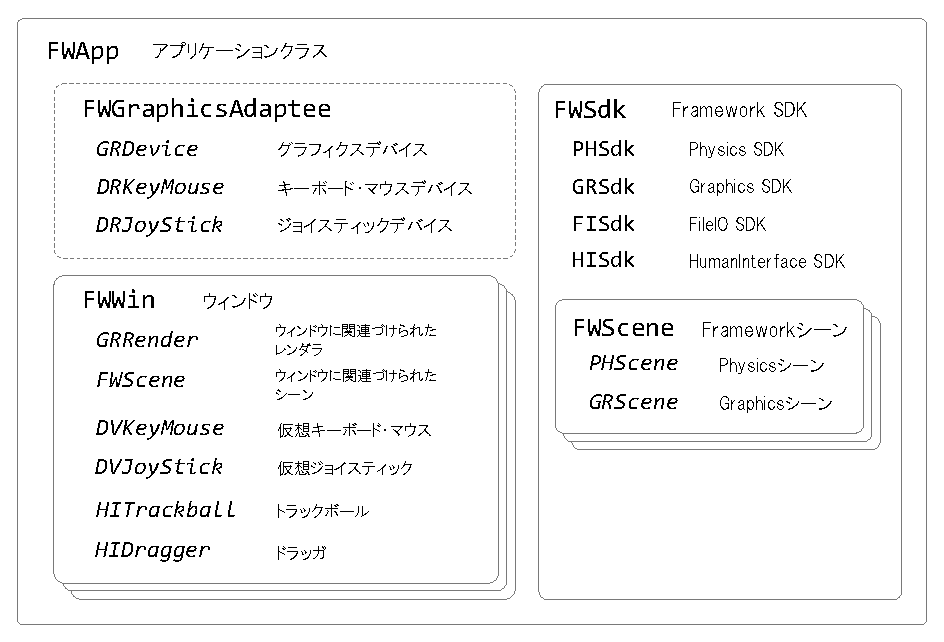
\includegraphics[width=.7\hsize]{fig/framework.eps}
\end{center}
\caption{Framework data structure}
\label{fig_framework}
\end{figure}


Framework�̓��W���[���Ԃ̘A�g�𑣐i���ăA�v���P�[�V�����̍쐬���x�����邽�߂̃��W���[���ł��D

Framework���W���[���̃f�[�^�\����Fig.\,\ref{fig_framework}�Ɏ����܂��D
�ŏ�ʂɂ̓A�v���P�[�V�����N���X\texttt{FWApp}������܂��D
���[�U��\texttt{FWApp}���p�����邱�ƂœƎ��̃A�v���P�[�V�������쐬���܂��D
\texttt{FWApp}���̒��Ƀg�b�v���x���E�B���h�E(\texttt{FWWin})�̔z��CFramework SDK (\texttt{FWSdk})�C
����уE�B���h�E�}�l�W��(\texttt{FWGraphicsAdaptee})�������܂��D

\texttt{FWWin}�̓g�b�v���x���E�B���h�E�ŁC���̃E�B���h�E�ɑΉ�������̓f�o�C�X��r���[�|�[�g����ێ����郌���_���C
���̃E�B���h�E�Ɗ֘A�t����ꂽ�V�[���ւ̎Q�ƂȂǂ������܂��D
�܂��C�}���ł͏ȗ�����Ă��܂����T�u�E�B���h�E��GUI�R���g���[�������‚��Ƃ��ł��܂��D

\texttt{FWSdk}�̖����͎��Ӄ��W���[���̋@�\�����ł��D
���̒��Ɏ��Ӄ��W���[����SDK�N���X��Framework�V�[��(\texttt{FWScene})�̔z��������܂��D

�E�B���h�E�}�l�W���͏����n�Ɉˑ�����f�o�C�X�̏�������C�x���g�n���h�����O���s���܂��D
�E�B���h�E�}�l�W���̓C���^�t�F�[�X�����J���Ă��܂���̂Ń��[�U�͂��̑��݂�z�Ɉӎ�����K�v�͂���܂���D
�}�ł̓f�[�^�\���̐����̂��߂ɂ����ċL�ڂ��Ă��܂��D

�ȉ��ł͌X�̍\���v�f�ɂ‚��Đ������Ă����܂��D


\section{Framework SDK}

\index{FWSdk}
Framework���W���[���̂��ׂẴI�u�W�F�N�g��SDK�N���X\texttt{FWSdk}�ɂ���ĊǗ�����܂��D
\texttt{FWSdk}�N���X�́C�v���O�����̎��s��ʂ��Ă����P�‚̃I�u�W�F�N�g�����݂���V���O���g���N���X�ł��D
\texttt{FWSdk}�I�u�W�F�N�g���쐬����ɂ͈ȉ��̂悤�ɂ��܂��D
\begin{sourcecode}
FWSdkIf* fwSdk = FWSdkIf::CreateSdk();
\end{sourcecode}
�ʏ킱�̑���̓v���O�����̏��������Ɉ�x�������s���܂��D
\texttt{FWSdk}���쐬����ƁC������\texttt{PHSdk}�C\texttt{GRSdk}�C\texttt{FISdk}�C\texttt{HISdk}���쐬����܂��D
���������Ă��������[�U���蓮�ō쐬����K�v�͂���܂���D
�e���W���[���̋@�\�ɃA�N�Z�X����ɂ͈ȉ��̊֐��ɂ��SDK���擾���܂��D

\noindent
\begin{tabular}{p{1.0\hsize}}
\\
\texttt{FWSdkIf}				\\ \midrule
\texttt{PHSdkIf* GetPHSdk()}	\\
Physics SDK���擾����D			\\
\\
\texttt{GRSdkIf* GetGRSdk()}	\\
Graphics SDK���擾����D		\\
\\
\texttt{FISdkIf* GetFISdk()}	\\
FileIO SDK���擾����D			\\
\\
\texttt{HISdkIf* GetHISdk()}	\\
HumanInterface SDK���擾����D	\\
\\
\end{tabular}

\section{Framework �V�[��}

\begin{figure}[t]
\begin{center}
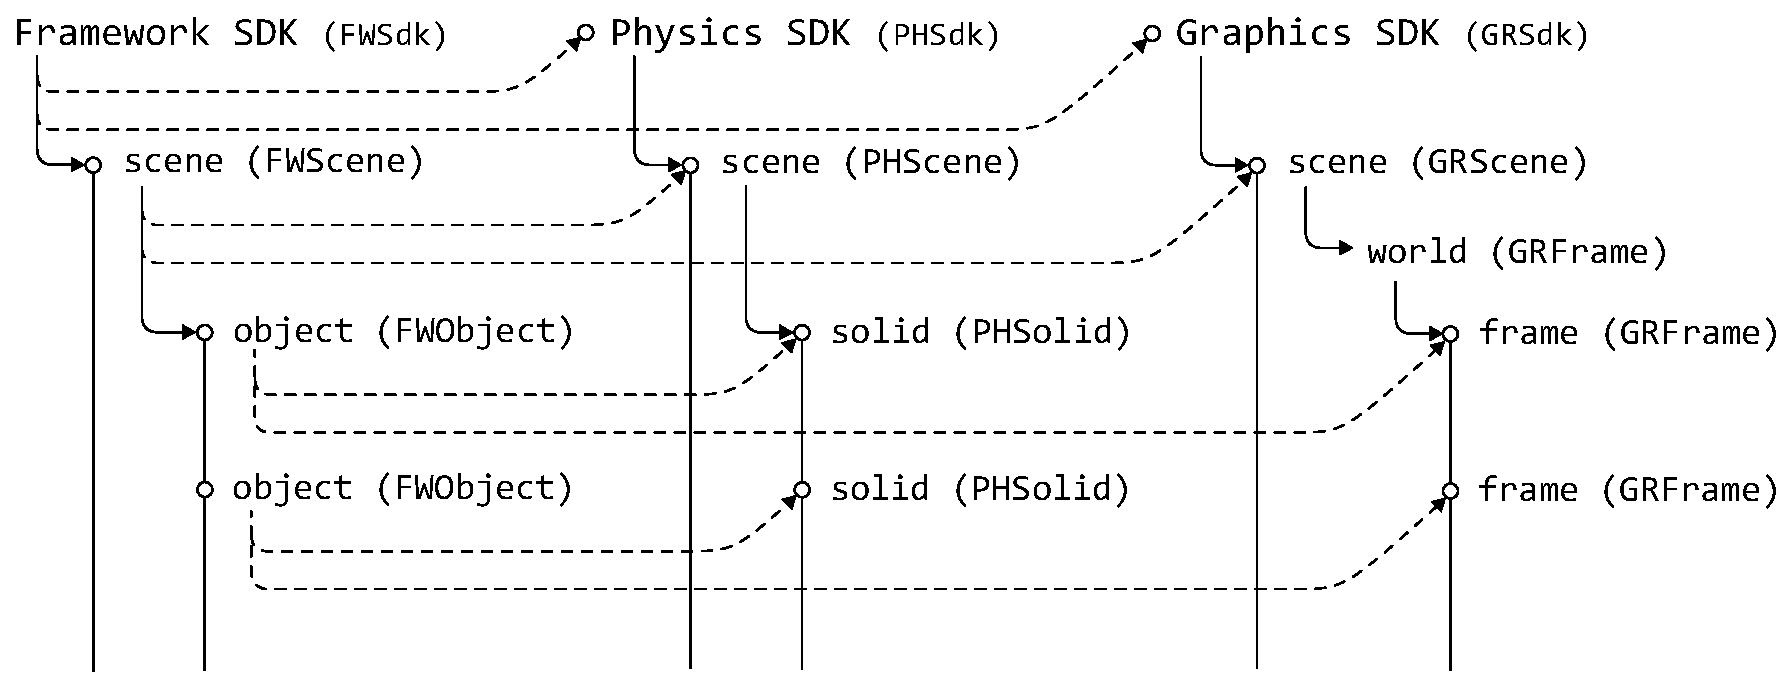
\includegraphics[width=.9\hsize]{fig/fwscene.eps}
\end{center}
\caption{Data structure of Framework, Physics and Graphics modules}
\label{fig_fwscene}
\end{figure}

\index{FWScene}
\index{FWObject}
Framework���W���[���̎�ȋ@�\��1�‚�Physics�V�[����Graphics�V�[���̓���������܂��D
Fig.\,\ref{fig_fwscene}��3�‚̃��W���[����SDK�ƃV�[���̊֌W�������܂��D
\texttt{FWSdk}�͔C�ӂ̐��̃V�[���i\texttt{FWScene}�N���X�j��ێ����܂��D
�܂��C�V�[���͔C�ӂ̐��̃I�u�W�F�N�g�i\texttt{FWObject}�N���X�j��ێ����܂��D
Fig.\,\ref{fig_fwscene}�Ɏ����悤�ɁC
�I�u�W�F�N�g��Physics���W���[���̍��̂�Graphics���W���[���̃g�b�v�t���[������Έ�ɑΉ��Â��܂��D
�����Ńg�b�v�t���[���Ƃ̓��[���h�t���[���̒����ɂ���t���[���̂��Ƃł��D
�����V�~�����[�V�����ɂ��v�Z����鍄�̂̉^�����t���[���̍��W�ϊ��ɔ��f�����邱�ƂŁC
�V�~�����[�V�����̗l�q��Graphics���W���[���̋@�\�𗘗p���ĉŽ������邱�Ƃ��ł���悤�ɂȂ�܂��D

�V�[���쐬�Ɋւ���\texttt{FWSdk}�̊֐����ȉ��Ɏ����܂��D

\noindent
\begin{tabular}{p{1.0\hsize}}
\\
\texttt{HITrackballIf}														\\ \midrule
\texttt{FWSceneIf* CreateScene(const PHSceneDesc\&, const GRSceneDesc\&)}	\\
�V�[�����쐬����D															\\
\\
\texttt{int NScene()}	\\
�V�[���̐����擾����	\\
\\
\texttt{FWSceneIf* GetScene(int i)}	\\
\texttt{i}�Ԗڂ̃V�[�����擾����D	\\
\\
\texttt{void MergeScene(FWSceneIf* scene0, FWSceneIf* scene1)}	\\
\texttt{scene1}�̎q�I�u�W�F�N�g��\texttt{scene0}�Ɉڂ��D		\\
\\
\end{tabular}

�V�[�����쐬����ɂ͈ȉ��̂悤�ɂ��܂��D
\begin{sourcecode}
FWSceneIf* fwScene = fwSdk->CreateScene();
\end{sourcecode}
\texttt{FWScene}���쐬����ƁC������\texttt{PHScene}��\texttt{GRScene}���쐬����C\texttt{FWScene}�ƃ����N����܂��D
\texttt{CreateScene}�Ƀf�B�X�N���v�^���w�肷�邱�Ƃ��ł��܂��D
\texttt{NScene}�͍쐬�����V�[���̐���Ԃ��܂��D

%�V�[���͂����‚ł��쐬�ł��܂����C���̒���1�‚̃V�[�����I�����ꂽ��Ԃɂ���܂��D
%�I�����ꂽ�V�[�����J�����g�V�[���ƌĂт܂��D
%�V�����쐬���ꂽ�V�[���̓J�����g�V�[���ƂȂ�܂��D
%�I����؂�ւ���ɂ�\texttt{SwitchScene}���g���܂��D

�V�[�����擾����ɂ�\texttt{GetScene}���g���܂��D
\texttt{GetScene}�Ɏw�肷�鐮���͍쐬���ꂽ���ԂɃV�[���ɗ^������ʂ��ԍ��ł��D
%�������ȗ�����ƃJ�����g�V�[�����Ԃ���܂��D
\begin{sourcecode}
fwSdk->CreateScene();               // create two scenes
fwSdk->CreateScene();
FWSceneIf *fwScene0, *fwScene1;
fwScene0 = fwSdk->GetScene(0);      // get 1st scene
fwScene1 = fwSdk->GetScene(1);      // get 2nd scene
\end{sourcecode}

\texttt{MergeScene}���g����2�‚̃V�[���𓝍�����1�‚̃V�[���ɂł��܂��D
\begin{sourcecode}
fwSdk->MergeScene(fwScene0, fwScene1);
\end{sourcecode}
��̃R�[�h�ł�\texttt{scene1}������\texttt{FWObject}��\texttt{scene0}�Ɉڂ���C�����ɃV�[�����Q�Ƃ���
\texttt{PHScene}��\texttt{GRScene}�Ɋւ��Ă����ꂼ���\texttt{MergeScene}�֐��ɂ�蓝�����s���܂��D

���ɁC\texttt{FWScene}�̊�{�@�\���ȉ��Ɏ����܂��D

\noindent
\begin{tabular}{p{.6\hsize}p{.3\hsize}}
\\
\texttt{FWSceneIf}													\\ \midrule
\texttt{void SetPHScene(PHSceneIf*)}	& Physics�V�[���̐ݒ�		\\
\texttt{PHSceneIf* GetPHScene()}		& Physics�V�[���̎擾		\\
\texttt{void SetGRScene(GRSceneIf*)}	& Graphics�V�[���̐ݒ�		\\
\texttt{GRSceneIf* GetGRScene()}		& Graphics�V�[���̎擾		\\
\texttt{FWObjectIf* CreateFWObject()}	& �I�u�W�F�N�g�̍쐬		\\
\texttt{int NObject()const}				& �I�u�W�F�N�g�̐�			\\
\texttt{FWObjectIf** GetObjects()}		& �I�u�W�F�N�g�z��̎擾	\\
\texttt{void Sync(bool)}				& ����						\\
\\
\end{tabular}

\texttt{[Set|Get][PH|GR]Scene}�֐��̓V�[���Ɋ��蓖�Ă�ꂽ\texttt{PHScene}��\texttt{GRScene}���擾������C�ʂ̃V�[�������蓖�Ă��肷��̂Ɏg�p���܂��D

\texttt{CreateFWObject}�֐���\texttt{FWObject}�I�u�W�F�N�g���쐬���܂��D
���̂Ƃ��C�V���ɍ쐬���ꂽ\texttt{FWObject}�ɂ�\texttt{PHSolid}�����\texttt{GRFrame}�͊��蓖�Ă��Ă��Ȃ���ԂɂȂ��Ă���̂Œ��ӂ��Ă��������D
�����������ɍ쐬����ɂ́C�ȉ��̃R�[�h��1�Z�b�g�Ŏ��s���܂��D

\begin{sourcecode}
FWObjectIf* fwObj = fwScene->CreateFWObject();
fwObj->SetPHSolid(fwScene->GetPHScene()->CreateSolid());
fwObj->SetGRFrame(
    fwScene->GetGRScene()->CreateVisual(GRFrameDesc())->Cast);
\end{sourcecode}

\texttt{Sync}�֐���\texttt{PHScene}��\texttt{GRScene}�̓����ɗp���܂��D
\begin{sourcecode}
fwScene->Sync(true);
\end{sourcecode}
�Ƃ���ƁC���̃V�[�����Q�Ƃ���\texttt{PHScene}���̍��̂̈ʒu�ƌ������C
���������̃V�[�����Q�Ƃ���\texttt{GRScene}���̃g�b�v�t���[���̈ʒu�ƌ����ɔ��f����܂��D
���̂Ƃ��̍��̂ƃg�b�v�t���[���Ƃ̑Ή��֌W��\texttt{FWObject}�ɂ���`����܂��D

�t��
\begin{sourcecode}
fwScene->Sync(false);
\end{sourcecode}
�Ƃ���ƁC���l�̃��J�j�Y���Ŋe�g�b�v�t���[���̈ʒu�ƌ������Ή����鍄�̂ɔ��f����܂��D

\section{�V�[���̃��[�h�ƃZ�[�u}

FileIO���W���[���𗘗p���ăV�[�������[�h�C�Z�[�u���邽�߂̊֐����p�ӂ���Ă��܂��D
�܂����[�h�ɂ͈ȉ��̊֐���p���܂��D

\noindent
\begin{tabular}{p{1.0\hsize}}
\\
\texttt{FWSdkIf}														\\ \midrule
\texttt{bool LoadScene(UTString path, ImportIf* imp, const IfInfo* ii, ObjectIfs* objs)}	\\
�V�[�������[�h����D		\\
\\
\end{tabular}

\texttt{path}�̓��[�h����t�@�C���ւ̃p�X���i�[����������ł��D
\texttt{imp}�ɂ̓C���|�[�g�����i�[���邽�߂�\texttt{Import}�I�u�W�F�N�g��^���܂��D
�C���|�[�g�����L������K�v�̂Ȃ��ꍇ��\texttt{NULL}�ō\���܂���D
\texttt{ii}�̓��[�h����t�@�C���̎�ނ𖾎����邽�߂̌^���ł��D
\texttt{NULL}���w�肷��ƃp�X�̊g���q���玩�����ʂ���܂��D
\texttt{objs}�̓��[�h�ɂ���č쐬�����I�u�W�F�N�g�c���[�̐e�I�u�W�F�N�g���i�[�����z��ł��D

���[�h�ɐ��������\texttt{true}�C���s�����\texttt{false}���Ԃ���܂��D
���[�h���ꂽ�V�[����\texttt{FWSdk}�̃V�[���z��̖����ɉ������܂��D

���ɁC�V�[�����Z�[�u����ɂ͈ȉ��̊֐����g���܂��D

\noindent
\begin{tabular}{p{1.0\hsize}}
\\
\texttt{FWSdkIf}														\\ \midrule
\texttt{bool SaveScene(UTString path, ImportIf* imp, const IfInfo* ii, ObjectIfs* objs)}	\\
�V�[�����Z�[�u����D		\\
\\
\end{tabular}

�����̈Ӗ���\texttt{LoadScene}�Ɠ��l�ł��D
\texttt{imp}�ɂ̓��[�h���ɋL�������C���|�[�g����^���܂��D
�ȗ�����ƃV�[���S�̂��P��̃t�@�C���ɃZ�[�u����܂��D

�Z�[�u�ɐ��������\texttt{true}�C���s�����\texttt{false}���Ԃ���܂��D


\section{Framework �I�u�W�F�N�g}

\texttt{FWObject}��\texttt{PHSolid}��\texttt{GRFrame}�̋��n������Ȗ����ł��̂ŁC���ꎩ�̂͂���قǑ����̋@�\�������Ă��܂���D


\section{�A�v���P�[�V�����N���X}

\index{FWApp}
Springhead�𗘗p����A�v���P�[�V�����̍쐬��e�Ղɂ��邽�߂ɁC�A�v���P�[�V�����N���X\texttt{FWApp}���p�ӂ���Ă��܂��D
\ref{sec_create_application}��\texttt{FWApp}���g���ĊȒP�ȃA�v���P�[�V�������쐬������@�ɂ‚��Đ������܂����̂ł���������킹�ĎQ�l�ɂ��Ă��������D

�`���Ő��������ʂ�CSpringhead�̂قƂ�ǂ̃I�u�W�F�N�g�́C�e�I�u�W�F�N�g��\texttt{Create}�n�֐����g���č쐬���܂����C
\texttt{FWApp}�͗�O�I�ɁCC++�̃N���X�p����p���ă��[�U�̃A�v���P�[�V�����N���X���`������@���Ƃ�܂��D
���̕������z�֐��ɂ���ē���̃J�X�^�}�C�Y���t���L�V�u���ɍs���邩��ł��D

�ȉ��ł�\texttt{FWApp}�̋@�\�⃆�[�U���������ׂ����z�֐��ɂ‚��ď��Ɍ��Ă����܂��D

\subsection*{������}

\texttt{FWApp}�̏����������͉��z�֐�\texttt{Init}�ōs���܂��D

\noindent
\begin{tabular}{p{.7\hsize}p{.2\hsize}}
\\
\texttt{FWApp}											\\ \midrule
\texttt{virtual void Init(int argc, char* argv[])}	&	\\
\\
\end{tabular}

�ȉ���\texttt{Init}�֐��̃f�t�H���g�̎����������܂��D

\begin{sourcecode}
void FWApp::Init(int argc, char* argv[]){
    // create SDK
    CreateSdk();
    // create a single scene
    GetSdk()->CreateScene();
    // initialize window manager
    GRInit(argc, argv);
    // create main window
    CreateWin();
    // create timer
    CreateTimer();
}
\end{sourcecode}
�͂��߂�
\begin{sourcecode}
    CreateSdk();
\end{sourcecode}
��SDK���쐬���܂��D
�‚���
\begin{sourcecode}
    GRInit(argc, argv);
\end{sourcecode}
�ŃE�B���h�E�}�l�W�����쐬����܂��D
�f�t�H���g�ł�GLUT��p����E�B���h�E�}�l�W�����쐬����܂��D
�����
\begin{sourcecode}
    GetSdk()->CreateScene();
\end{sourcecode}
��\texttt{FWScene}��1�쐬���܂��D
�‚Â���
\begin{sourcecode}
    CreateWin();
\end{sourcecode}
�Ń��C���E�B���h�E���쐬���܂��D
�Ō��
\begin{sourcecode}
    CreateTimer();
\end{sourcecode}
�Ń^�C�}���쐬���܂��D

���̊�{�����ɒlj����ĂȂ�炩�̏������s���ꍇ��
\begin{sourcecode}
virtual void Init(int argc = 0, char* argv[] = 0){
    // select GLUI window manager
    SetGRAdaptee(TypeGLUI);

    // call base Init
    FWApp::Init(argc, argv);

    // do extra initialization here


}
\end{sourcecode}
�̂悤�ɁC\texttt{FWApp:Init}�����s���Ă���lj��̏������s���̂��ǂ��ł��傤�D
����C�ȉ��ɋ�����悤�ȃJ�X�^�}�C�Y���K�v�ȏꍇ��\texttt{Init}�֐��̏����S�̂�h���N���X�ɋL�q����K�v������܂��D
\begin{itemize}
\item �V�[���������J�X�^�}�C�Y������
\item �E�B���h�E�̏����T�C�Y��^�C�g����ύX������
\item �قȂ��ނ̃^�C�}���g������
\end{itemize}
���̏ꍇ�́C��ɍڂ���\texttt{Init}�̃f�t�H���g���������ƂɕK�v�ȕ����ɏC����������̂��ǂ��ł��傤�D

�v���O�����̑S�̂̍\���͒ʏ�ȉ��̂悤�ɂȂ�܂��D

\begin{sourcecode}
MyApp app;

int main(int argc, char* argv[]){
    app.Init(argc, argv);
    app.StartMainLoop();
    return 0;
}
\end{sourcecode}

������\texttt{MyApp}�̓��[�U����`����\texttt{FWApp}�̔h���N���X�ł��i������񑼂̖��O�ł��\���܂���j�D
\texttt{MyApp}�̃C���X�^���X���O���[�o���ϐ��Ƃ��Ē�`���C
\texttt{main}�֐���\texttt{Init}�C\texttt{StartMainLoop}���������s���܂��D
\texttt{StartMainLoop}�֐��̓A�v���P�[�V�����̃��C�����[�v���J�n���܂��D


\subsection*{�^�C�}}

�^�C�}�̍쐬�ɂ�\texttt{CreateTimer}�֐����g���܂��D
�ʏ�C\texttt{CreateTimer}��\texttt{Init}�̒��ŌĂт܂��D

\noindent
\begin{tabular}{p{.7\hsize}p{.2\hsize}}
\\
\texttt{FWApp}												\\ \midrule
\texttt{UTTimerIf* CreateTimer(UTTimerIf::Mode mode)}	&	\\
\\
\end{tabular}

����\texttt{mode}�Ɏw��ł���l��\texttt{UTTimer}��\texttt{SetMode}�Ɠ����ł��D
\ref{sec_uttimer}�߂��Q�Ƃ��Ă��������D
�߂�l�Ƃ���\texttt{UTTimer}�̃C���^�t�F�[�X���Ԃ���܂��D
�����Ȃǂ̐ݒ�͂��̃C���^�t�F�[�X����čs���܂��D

�V�~�����[�V�����p�ƕ`��p��2�‚̃^�C�}���쐬�������ȉ��Ɏ����܂��D
\begin{sourcecode}
UTTimerIf *timerSim, *timerDraw;
timerSim = CreateTimer(MULTIMEDIA);
timerSim->SetInterval(10);
timerDraw = CreateTimer(FRAMEWORK);
timerDraw->SetInterval(50);
\end{sourcecode}
���̗�ł̓V�~�����[�V�����p�ɂ͎�����$10$[ms]�̃}���`���f�B�A�^�C�}���g���C
�`��p�ɂ͎���$50$[ms]�̃t���[�����[�N�^�C�}�iGLUT�^�C�}�j���g���Ă��܂��D

�^�C�}���n������ƁC�������ƂɈȉ��̉��z�֐����Ă΂�܂��D

\noindent
\begin{tabular}{p{.7\hsize}p{.2\hsize}}
\\
\texttt{FWApp}								\\ \midrule
\texttt{virtual void TimerFunc(int id)}	&	\\
\\
\end{tabular}
�^�C�}�̔��ʂ͈���$id$�ōs���܂��D

\texttt{TimerFunc}�̃f�t�H���g�̐U�镑���ł́C
�J�����g�E�B���h�E�̃V�[����\texttt{Step}���ĂсC�‚���\texttt{PostRedisplay}�ōĕ`��v���𔭍s���܂�
�i���̌��ʁC�����\texttt{Display}�֐����Ăяo����܂��j�D
���̐U�镑�����J�X�^�}�C�Y�������ꍇ��\texttt{TimerFunc}�֐����I�[�o���C�h���܂��D
\begin{sourcecode}
void TimerFunc(int id){
    // proceed simulation of scene attached to current window
    if(id == timerSim->GetID()){
        GetCurrentWin()->GetScene()->Step();
    }
    // generate redisplay request
    else if(id == timerDraw->GetID()){
        PostRedisplay();
    }
}
\end{sourcecode}
���̗�ł̓V�~�����[�V�����ƕ`��ɈقȂ�2�‚̃^�C�}���g�p���Ă��܂��D

\subsection*{�`��}

�`�揈���͎��̉��z�֐��ōs���܂��D

\noindent
\begin{tabular}{p{.7\hsize}p{.2\hsize}}
\\
\texttt{FWApp}						\\ \midrule
\texttt{virtual void Display()}	&	\\
\\
\end{tabular}

\texttt{Display}�͕`��v�������s���ꂽ�Ƃ��ɌĂяo����܂��D
�`��v����\texttt{PostRedisplay}�֐��ōs���܂��D

\noindent
\begin{tabular}{p{.7\hsize}p{.2\hsize}}
\\
\texttt{FWApp}							\\ \midrule
\texttt{virtual void PostRedisplay()}	&	\\
\\
\end{tabular}

\texttt{Display}�֐��̃f�t�H���g�̐U�镑���ł̓J�����g�E�B���h�E��\texttt{Display}�֐����Ă΂�܂��D

\subsection*{�L�[�{�[�h�E�}�E�X�C�x���g}

\texttt{FWApp}�͊e�E�B���h�E�Ɋ֘A�t����ꂽ���z�L�[�{�[�h�E�}�E�X�f�o�C�X\texttt{DVKeyMouse}�ɃR�[���o�b�N�o�^����Ă��܂��D
���������Ĉȉ��̉��z�֐����I�[�o���C�h���邱�ƂŃL�[�{�[�h�E�}�E�X�C�x���g�������ł��܂��D

\noindent
\begin{tabular}{p{1.0\hsize}}
\\
\texttt{FWApp}							\\ \midrule
\texttt{virtual bool OnMouse(int button, int state, int x, int y)}	\\
\texttt{virtual bool OnDoubleClick(int button, int x, int y)}	\\
\texttt{virtual bool OnMouseMove(int state, int x, int y, int zdelta)}	\\
\texttt{virtual bool OnKey(int state, int key, int x, int y)}	\\
\\
\end{tabular}

�e�C�x���g�n���h���̏ڍׂɂ‚��Ă�\ref{sec_hi_keymouse}�߂��Q�Ƃ��ĉ������D

\section{�E�B���h�E}

�E�B���h�E�₻�̑���GUI�R���g���[���̍쐬��Framework�ɂ���ăT�|�[�g����Ă��܂��D
���łɏq�ׂĂ����Ƃ���C\texttt{FWApp}�̓g�b�v���x���E�B���h�E�̔z��������܂��D




\section{Framework��p�����V�~�����[�V�����ƕ`��}

Framework���W���[������ĕ����V�~�����[�V�������s���ɂ͈ȉ��̊֐����g���܂��D

\noindent
\begin{tabular}{p{.7\hsize}p{.2\hsize}}
\\
\texttt{FWSdkIf}			\\ \midrule
\texttt{void Step()}	& 	\\
\end{tabular}
\noindent

\texttt{FWSdk}��\texttt{Step}�̓A�N�e�B�u�V�[����\texttt{Step}���Ăт܂��D
����������\texttt{GetScene()->Step()}�Ɠ����ł��D
���\texttt{FWScene}��\texttt{Step}�́C�ێ����Ă���\texttt{PHScene}��\texttt{Step}���Ăт܂��D
����������\texttt{GetPHScene()->Step()}�Ɠ����ł��D
�����Ƃ��������b�p�[�֐��ł����C���[�U�̃^�C�v�񐔐ߖ�̂��߂ɗp�ӂ���Ă��܂��D

Framework��p�����`��ɂ�2�ʂ�̕��@������܂��D
1�‚�Graphics�̃V�[���O���t��p������@�C����1�‚�Physics�V�[���𒼐ڕ`�悷����@�ł��D
��҂̓f�o�b�O�`��Ƃ��Ă΂�Ă��܂��D

\noindent
\begin{tabular}{p{.7\hsize}p{.2\hsize}}
\\
\texttt{FWSdkIf}						\\ \midrule
\texttt{void Draw()}				&	\\
\texttt{void SetDebugMode(bool)}	& 	\\
\texttt{bool GetDebugMode()}		&	\\
\\
\end{tabular}

\texttt{Draw}�֐��͕`�惂�[�h�ɉ������`�揈�����s���܂��D
\texttt{Draw}�͒ʏ�A�v���P�[�V�����̕`��n���h������Ăяo���܂��D
\texttt{[Set|Get]DebugMode}�͒ʏ�`�惂�[�h(\texttt{false})�ƃf�o�b�O�`�惂�[�h(\texttt{true})��؂�ւ��܂��D

�ʏ�`�惂�[�h�ɂ�����\texttt{Draw}�֐����ĂԂƁC
�͂��߂ɃA�N�e�B�u�V�[���ɂ‚���\texttt{Sync(true)}���Ă΂�C���̂̏�Ԃ��V�[���O���t�ɔ��f����܂��D
���ɃA�N�e�B�u�V�[�����Q�Ƃ���\texttt{GRScene}��\texttt{Render}�֐����Ă΂�C�V�[���O���t���`�悳��܂��D
���̕��@�ł̓V�[���O���t�����ƒ��C�g��e�N�X�`���Ȃǂ̏����ő�����p���ăt�H�g���A���X�e�B�b�N�ȕ`�悪�”\�ł��D
���̔��ʁC�����V�~�����[�V��������ړI�ł���ꍇ�ɂ̓V�[���O���t�̍\�z�Ƃ����t���I�ȃR�X�g���x����Ȃ���΂Ȃ�Ȃ��Ƃ����f�����b�g������܂��D

�f�o�b�O�`��ɂ‚��Ă͎��߂Ő������܂��D

\section{�f�o�b�O�`��}

�f�o�b�O�`�惂�[�h�ł�\texttt{PHScene}�̏�񂾂���p���ĕ`�悪�s����̂ŁC�V�[���O���t�\�z�̎�Ԃ��Ȃ��܂��D
�܂��C���̂ɉ����͂Ȃǂ̕����V�~�����[�V�����Ɋւ�������Ž������邱�Ƃ��ł��܂��D
����ŁC�\��F�����g���Ȃ��ȂǁC�`��̎��R�x�ɂ͈��̐��񂪐����܂��D

�f�o�b�O�`�惂�[�h�ł�\texttt{FWScene}��\texttt{DrawPHScene}�֐��ɂ��`�揈�����s���܂��D

\noindent
\begin{tabular}{p{.7\hsize}p{.2\hsize}}
\\
\texttt{FWSceneIf}									\\ \midrule
\texttt{void DrawPHScene(GRRenderIf* render)}	&	\\
\\
\end{tabular}

\texttt{DrawPHScene}�́C�e���̂Ɋ��蓖�Ă��Ă���Փ˔���`��C���W���C��p���Ă���́C�ڐG�f�ʂȂǂ�`�悵�܂��D
���ڕʂɕ`����s������C�`��F��ݒ肷��ɂ͌�q����`�搧��֐���p���܂��D

\subsection*{�f�o�b�O�`�掞�̃J�����ƃ��C�g}

�f�o�b�O�`��ɂ����Ă��J�����̏���\texttt{GRScene}���Q�Ƃ���܂��D
����\texttt{GRScene}���J������ۗL���Ă���ꍇ�͂��̃J������\texttt{Render}���Ă΂�C���_�Ɠ��e�ϊ����ݒ肳��܂��D
\texttt{GRScene}���J�����������Ȃ��ꍇ�͎蓮�Őݒ肷��K�v������܂��D

���C�g�ɂ‚��ẮC�����O���Ń����_���ɑ΂��ă��C�g�ݒ肪����Ă���ꍇ�͂��̐ݒ肪�D�悳��C
�����_����1�‚����C�g�������Ȃ��ꍇ�͓����Ńf�t�H���g���C�g���ݒ肳��܂��D

\subsection*{�•ʂ̕`��}

�ȉ��̊֐���\texttt{DrawPHScene}����Ăяo����܂����C���[�U���•ʂɌĂяo�����Ƃ��ł��܂��D

\noindent
\begin{tabular}{p{.7\hsize}p{.2\hsize}}
\\
\texttt{FWSceneIf}												\\ \midrule
\texttt{void DrawSolid(GRRenderIf*, PHSolidIf*, bool)}		&	���̂�`��\\
\texttt{void DrawShape(GRRenderIf*, CDShapeIf*, bool)}		&	�`���`��\\
\texttt{void DrawConstraint(GRRenderIf*, PHConstraintIf*)}	&	�S����`��\\
\texttt{void DrawContact(GRRenderIf*, PHContactPointIf*)}	&	�ڐG��`��\\
\texttt{void DrawIK(GRRenderIf*, PHIKEngineIf*)}			&	IK����`��\\
\\
\end{tabular}

\subsection*{�`�搧��}

�ȉ��̊֐��͕`���On/Off��؂�ւ��܂��D

\noindent
\begin{tabular}{p{.8\hsize}p{.1\hsize}}
\\
\texttt{FWSceneIf}													\\ \midrule
\texttt{void SetRenderMode(bool solid, bool wire)}					&	\\
\texttt{void EnableRender(ObjectIf* obj, bool enable)}				&	\\
\texttt{void EnableRenderAxis(bool world, bool solid, bool con)}	&	\\
\texttt{void EnableRenderForce(bool solid, bool con)}				&	\\
\texttt{void EnableRenderContact(bool enable)}						&	\\
\texttt{void EnableRenderGrid(bool x, bool y, bool z)}				&	\\
\texttt{void EnableRenderIK(bool enable)}							&	\\
\\
\end{tabular}

\texttt{SetRenderMode}�̓\���b�h�`��i�ʂ�h��‚Ԃ��j�ƃ��C���t���[���`��i�ʂ̗֊s�j��On/Off��؂�ւ��܂��D

\texttt{EnableRender}�͎w�肵���I�u�W�F�N�g�̕`���On/Off��؂�ւ��܂��D
���ڂł͂Ȃ��I�u�W�F�N�g���x���ŕ`�搧�䂵�����ꍇ�ɕ֗��ł��D
\texttt{obj}�Ɏw��ł���͍̂���(\texttt{PHSolidIf*})���S��(\texttt{PHConstraintIf*})�ł��D

\texttt{EnableRenderAxis}�͍��ڕʂɍ��W���̕`���ݒ肵�܂��D
\texttt{world}�̓��[���h���W���C\texttt{solid}�͍��́C\texttt{con}�͍S���̍��W���ł��D

\texttt{EnableRenderForce}�͗͂ƃ��[�����g�̕`���ݒ肵�܂��D
\texttt{solid}�͍��̂ɉ����́i�������O�݂͂̂ōS���͂͏����j�C\texttt{con}�͍S���͂ł��D

\texttt{EnableRenderGrid}�͊e���Ɋւ��ăO���b�h�̕`���ݒ肵�܂��D

\texttt{EnableRenderIK}��IK���̕`���ݒ肵�܂��D

�ȉ��̊֐��͕`�摮�����w�肷��̂Ɏg���܂��D

\noindent
\begin{tabular}{p{.8\hsize}p{.1\hsize}}
\\
\texttt{FWSceneIf}																\\ \midrule
\texttt{void SetSolidMaterial(int mat, PHSolidIf* solid)}						&	\\
\texttt{void SetWireMaterial (int mat, PHSolidIf* solid)}						&	\\
\texttt{void SetAxisMaterial(int matX, int matY, int matZ)}						&	\\
\texttt{void SetAxisScale(float world, float solid, float con)}					&	\\
\texttt{void SetAxisStyle(int style)}											&	\\
\texttt{void SetForceMaterial(int matForce, int matMoment)}						&	\\
\texttt{void SetForceScale(float scaleForce, float scaleMoment)}				&	\\
\texttt{void SetContactMaterial(int mat)}										&	\\
\texttt{void SetGridOption(char axis, float offset, float size, int slice)}		&	\\
\texttt{void SetGridMaterial(int matX, int matY, int matZ)}						&	\\
\texttt{void SetIKMaterial(int mat)}											&	\\
\texttt{void SetIKScale(float scale)}											&	\\
\\
\end{tabular}

\texttt{SetSolidMaterial}�͎w�肵�����̂̃\���b�h�`��F���w�肵�܂��D
\texttt{mat}�Ɏw��ł���l��\ref{sec_grmaterial}�߂ŏq�ׂ��\��F�ł��D
\texttt{solid}��\texttt{NULL}���w�肷��Ƃ��ׂĂ̍��̂̐F���w�肳�ꂽ�l�ɂȂ�܂��D
\texttt{SetWireMaterial}�͓��l�ɍ��̂̃��C���t���[���`��F���w�肵�܂��D

\texttt{SetAxisMaterial}�͍��W���̐F��x, y, z�•ʂɎw�肵�܂��D
\texttt{SetAxisScale}�͍��W���̏k�ڂ��w�肵�܂��D
\texttt{SetAxisStyle}�͍��W���̃X�^�C�����w�肵�܂��D

\texttt{SetForceMaterial}�C\texttt{SetForceScale}�͂��ꂼ��́i���i�͂ƃ��[�����g�j�̕`��F�Ək�ڂ��w�肵�܂��D

\texttt{SetContactMaterial}�͐ڐG�f�ʂ̕`��F���w�肵�܂��D

\texttt{SetGridOption}�̓O���b�h�̃I�v�V�������w�肵�܂��D
\texttt{SetGridMaterial}�̓O���b�h�̕`��F���w�肵�܂��D

\texttt{SetIKMaterial}�C\texttt{SetIKScale}��IK���̕`��F�Ək�ڂ��w�肵�܂��D


\section{�͊o�C���^���N�V�����̂��߂̃A�v���P�[�V����}
Springhead2�ɂ̓V�[���Ƃ̗͊o�C���^���N�V�����̂��߂̃G���W��\texttt{PHHapticEngine}���܂܂�Ă��܂��D
�����ł͗͊o�C���^���N�V�����̂��߂̃A�v���P�[�V�����̍쐬���@�ɂ‚��Đ������܂��D
�܂��́C�ʏ��\texttt{Framework}�A�v���P�[�V�����̍쐬�Ɠ��l�ɁC�ЂȌ`�N���X�ł���\texttt{FWApp}���p�����ăA�v���P�[�V������
�쐬���܂��D
�����āC\texttt{Init}�֐����ŗ͊o�C���^���N�V������L�����ƁC�͊o�C���^���N�V�����V�X�e���̃��[�h��ݒ肵�܂��D
\begin{sourcecode}
	// given PHSceneIf* phScene,
    phScene->GetHapticEngine()->EnableHapticEngine(true);
    phScene->GetHapticEngine()->
    SetHapticEngineMode(PHHapticEngineDesc::MULTI_THREAD);
\end{sourcecode}
�͊o�C���^���N�V�����V�X�e���̃��[�h��
�V���O���X���b�h�A�v���P�[�V�����̂��߂�\texttt{SINGLE\_THREAD}�C
�}���`���f�B�A�A�v���P�[�V�����̂��߂�\texttt{MULTI\_THREAD}�C�Ǐ��V�~�����[�V�����𗘗p����\texttt{LOCAL\_DYNAMICS}��3��ނ�����܂��D
�W���ł�\texttt{MULTI\_THREAD}���ݒ肳��Ă��܂��D
\texttt{MULTI\_THREAD}�C\texttt{LOCAL\_DYNAMICS}�̃��[�h�̓}���`�X���b�h�𗘗p�����A�v���P�[�V�����ƂȂ�C
�����V�~�����[�V���������s���镨���X���b�h�C�͊o�����_�����O�����s����͊o�X���b�h������ɓ����܂��D
���̂��߁C���ꂼ��̃X���b�h���R�[���o�b�N���邽�߂Ƀ^�C�}��ݒ肵�����K�v������܂��D
\clearpage

\begin{sourcecode}
	// given PHSceneIf* phScene,
	int physicsTimerID, hapticTimerID // �e�^�C�}��ID
	// FWApp::TimerFunc���I�[�o���C�h�����R�[���o�b�N�֐�
	void MyApp::TimerFunc(int id){
        if(hapticTimerID == id){
            // �͊o�X���b�h�̃R�[���o�b�N
            phScene->StepHapticLoop();	
        }else{
            // �����X���b�h�̃R�[���o�b�N
            phScene->GetHapticEngine()->StepPhysicsSimulation();	
            PostRedisplay();	// �`��
        }	
	}	
\end{sourcecode}


���Ƀ��[�U���I�u�W�F�N�g�ƃC���^���N�V�������邽�߂̃|�C���^�C�͊o�|�C���^\texttt{PHHapticPointer}�����܂��D
�����āC�ǂ̃C���^�t�F�[�X�ƌ�������̂���ݒ肵�܂��D
\texttt{PHHapticPointer}��\texttt{PHScene}�����邱�Ƃ��ł��܂��D
\texttt{PHHapticPointer}��\texttt{PHSolid}���p�������N���X��\texttt{PHSolid}�̊֐��𗘗p���āC
���ʁC�����e���\���C�`��Ȃǂ����킹�Đݒ肵�܂��D
�Ⴆ��Spidar-G6�Ɛڑ�����ꍇ�ɂ́C

\begin{sourcecode}
	// given PHSceneIf* phScene,
	// given HISpidarIf* spg,
    PHHapticPointerIf* pointer = phScene->CreateHapticPointer();
    /*
        ���ʁC�����e���\���C�`��Ȃǂ�ݒ肷��
    */
    pointer->SetHumanInterface(spg);
\end{sourcecode}
�Ƃ��܂��D
�����PHHapticPointer�ɂ‚��Ĉȉ��̊֐���p���āC�͊o�񎦂̂��߂̃p�����[�^��ݒ肵�܂��D

\noindent
\begin{tabular}{p{.8\hsize}p{.1\hsize}}
\\
\texttt{PHHapticPointerIf}													\\ \midrule
\texttt{void SetHumanInterface(HIBaseIf* interface)}						&	\\
\texttt{void SetDefaultPose(Posed pose)}									&	\\
\texttt{void SetPosScale(double scale)}										&	\\
\texttt{void SetReflexSpring(float s)}										&	\\
\texttt{void SetReflexDamper(float s)}										&	\\
\texttt{void EnableFriction(bool b)}										&	\\
\texttt{void EnableVibration(bool b)}										&	\\
\texttt{void SetLocalRange(float s)}										&	\\
\texttt{void SetHapticRenderMode(PHHapticPointerDesc::HapticRenderMode m )}	&	\\
\\
\end{tabular}

\texttt{SetHumanInterface}�͗͊o�|�C���^�Ƀq���[�}���C���^�t�F�[�X�����蓖�Ă܂��D
\texttt{SetDefaultPose}�̓V�[�����ł̗͊o�|�C���^�̏����ʒu���w�肵�܂��D
\texttt{SetPosScale}�̓V�[�����ł̗͊o�|�C���^�̉“��X�P�[�����w�肵�܂��D
\texttt{SetReflexSpring}�͗͊o�����_�����O�i���͌v�Z�j�̂��߂̃o�l�W���l��ݒ肵�܂��D
\texttt{SetReflexDamper}�͗͊o�����_�����O�̂��߂̃_���p�W���l��ݒ肵�܂��D
\texttt{EnableFriction}�͗͊o�|�C���^�̖��C�͒񎦂�L�������܂��D
\texttt{EnableVibration}�͗͊o�|�C���^�̐U���񎦂�L�������܂��D
\texttt{SetLocalRange}�͋Ǐ��V�~�����[�V�����V�X�e�����g�p���̋Ǐ��V�~�����[�V�����͈͂��w�肵�܂��D
\texttt{SetHapticRenderMode}�͗͊o�����_�����O�̃��[�h���w�肵�܂��D

�Ō��\texttt{SetHapticRenderMode}�ɂ�\texttt{PENALTY}�C\texttt{CONSTRAINT}�̃��[�h������܂��D
\texttt{PENALTY}�͗͊o�|�C���^�����̂ɐڐG�������̊e�ڐG�_�̐N���ʂƃo�l�_���p�W�����悶�����̂𑫂����킹�����̂�
���͂Ƃ��Čv�Z����C�C���^�t�F�[�X����o�͂���܂��D\texttt{CONSTRAINT}�͗͊o�|�C���^�����̂ɐN�����Ă��Ȃ���ԁi�v���L�V�j��
���߁C�͊o�|�C���^�ƃv���L�V�̋����̍����Ƀo�l�_���p�W�����悶�����̂𔽗͂Ƃ��Čv�Z���܂��D


\chapter{Python����Ƃ̘A�g}
\label{chap_embpython}
% ----- ----- ----- ----- ----- ----- ----- ----- ----- ----- ----- ----- ----- ----- ----- ----- ----- ----- ----- -----
%
% ���h�L�������g�̏�������

% �@�\ ::= "�T��" �� �ڍ� ���t�@�����X*
% ��   ::= ["�R�[�h��" "�R�[�h��̐���"]*
% �ڍ� ::= [�@�\]*

% ���t�@�����X ::= [�f�B�X�N���v�^ | �C���^�t�F�[�X]

% - �����Ƃ��ă��t�@�����X�͋@�\�̂܂Ƃ߂ƕ��ɂƂǂ߂�D
% - Getter/Setter�͑Ή�����f�B�X�N���v�^�̃��t�@�����X�ɏ����C�C���^�t�F�[�X�̃��t�@�����X�ɂ͍ڂ��Ȃ��D
% - �}�� "�T��" "�R�[�h��" "�R�[�h��̐���" �œK�X�p����D������ "�R�[�h��" �̐}�͌����Ƃ��Ă��̃R�[�h�̎��s���ʂƂ���D

%
% ----- ----- ----- ----- ----- ----- ----- ----- ----- ----- ----- ----- ----- ----- ----- ----- ----- ----- ----- -----


% ----- ----- ----- ----- ----- ----- ----- ----- ----- ----- ----- ----- ----- ----- ----- ----- ----- -----
%
% �T��
% 
\begin{chapterabstract}
EmbPython���W���[���́C�X�N���v�g����Python�Ƃ̘A�g�@�\��񋟂��܂��DPython�C���^�v���^����Springhead�̋@�\���Ăяo������CSpringhead�A�v���P�[�V������Python�C���^�v���^��g�ݍ���ŃX�N���v�e�B���O�G���W���Ƃ��Ďg�p����Ƃ����������ł��܂��D

EmbPython���W���[���̎g�p�ɂ��CPython�C���^�v���^���Springhead API�N���X�ւ̃C���^�t�F�[�X�N���X���񋟂���܂��D���[�U��Python�C���^�t�F�[�X�N���X���g�p����Springhead�̊e�@�\�ɃA�N�Z�X���܂��DPython�C���^�t�F�[�X�N���X�͓����I��Springhead�̋@�\���Ăяo���C���ʂ�Python�C���^�t�F�[�X�N���X�ɕϊ����ĕԂ��܂��D
\end{chapterabstract}

% ----- ----- ----- ----- ----- ----- ----- ----- ----- ----- ----- ----- ----- ----- ----- ----- ----- -----
%
% �ڍׂP
% 
\section{���p�@}

�傫�������ē�ʂ�̗��p�@��z�肵�Ă��܂��D

��‚́CC++�Ŏ������ꂽSpringhead�A�v���P�[�V�����ɑ΂��CPython�C���^�v���^��g�ݍ��ނ��Ƃł��DSpringhead�A�v���P�[�V�����̋@�\�̈ꕔ��Python�X�N���v�g�L�q���C�g���������߂܂��D

������‚́CPython�C���^�v���^�ɑ΂���O���g�����W���[��(Python DLL, pyd)�Ƃ��Ē񋟂��ꂽSpringhead�𗘗p���邱�ƂŁCPython�A�v���P�[�V������Springhead�̋@�\��g�ݍ��ޗ��p�@�ł��D

�ǂ���̏ꍇ�ɂ����Ă��CEmbPython���W���[����Python������Springhead�̊֐����Ăяo�����߂̃C���^�t�F�[�X��񋟂��܂��D�֌W��\Fig{epoverview}�Ɏ����܂��D

\begin{fig}
\epscapopt{epoverview}{Python�A�g��EmbPython���W���[���̈ʒu�Â�}{width=0.8\hsize}
\end{fig}

\subsection{�‹��ϐ�PATH�̐ݒ�}

Springhead�̓���́A\path{Springhead2\core\bin\win64}�t�H���_�A�����\path{Springhead2\dependency\bin\win64}�t�H���_����dll�Q�Ɉˑ����Ă��܂��B�����̃t�H���_�̐�΃p�X���‹��ϐ�PATH�ɒlj����Ă��������B


% ----- ----- ----- ----- ----- ----- ----- ----- ----- ----- ----- ----- ----- ----- ----- ----- 
% �ڍ�a
\subsection*{Springhead�ւ�Python�g����}

Springhead�A�v���P�[�V������Python�C���^�v���^��g�ݍ���ŗ��p������@��������܂��D
�{�߂ł͂܂�Springhead�ɓ������ꂽPython�C���^�v���^�g�ݍ��݃T���v�����Љ�C�ȒP�Ȏg������������܂��D���̌�C�T���v���ɂ�����Python�C���^�v���^�g�ݍ��݂̂��߂̃\�[�X�R�[�h�ɂ‚��ĉ�����܂��D

\subsubsection*{PythonSpr�T���v���̃r���h�Ǝ��s}

Python�C���^�v���^�g�ݍ��݃T���v���� \path{src\Samples\EmbPython\PythonSpr} �ɂ���܂��D
�r���h����� \path{PythonSpr.exe} ���ł��܂��D

\texttt{PythonSpr}�T���v���͕W���I��Springhead�T���v���A�v���P�[�V�����t���[�����[�N��Python�C���^�v���^��g�ݍ��񂾂��̂ŁC�����V�[�����\�z�E�V�~�����[�V�����E�`�悷�鎖���ł��܂��DPython�C���^�v���^�����\texttt{phSdk}��\texttt{fwSdk}�ɃA�N�Z�X���邱�Ƃ��ł��C�\���@�\��؂�ւ�����V�[���ɃI�u�W�F�N�g���쐬������Ƃ��������Ƃ�Python����s���܂��D

���s�̑O�ɁC�‹��ϐ���ݒ肵�܂��D����́CSpringhead�A�v���P�[�V�����ɑg�ݍ��܂ꂽPython�C���^�v���^��Python�̕W�����C�u�����Q�ɃA�N�Z�X���邽�߂ɕK�v�ł��D
\begin{description}
\item[\texttt{SPRPYTHONPATH}�‹��ϐ�]~

Springhead�����[�X��W�J�����t�H���_����\path{bin\src\Python32\Lib}�ւ̃t���p�X���w�肵�܂��DPython3.2��\path{c:\Python32}�ɃC���X�g�[�����Ă���ꍇ�C\path{C:\Python32\Lib}�ł����܂��܂���D
\end{description}

\path{PythonSpr.exe}�����s����Ǝ��̂悤�ȉ�ʂ�����܂��D

���X�N���[���V���b�g��

�E��Springhead�̎��s��ʁC���̃R���\�[����Python�v�����v�g�ł��D�N�����ɂ́CSpringhead���s��ʂɂ͉��̃V�[�����\�z����Ă��Ȃ����߁C���[���h���W�n���������݂̂��`�悳��Ă��܂��D

����@�͈ȉ��̒ʂ�ł��D
\begin{description}
\item[�}�E�X ���h���b�O] ���_�ύX�i��]�j
\item[�}�E�X �E�h���b�O] ���_�ύX�i�g��k���j
\item[�X�y�[�X�L�[] �V�~�����[�V�����J�n�E�ꎞ��~�i�N������͒�~���Ă��܂��j
\end{description}

\subsubsection*{PythonSpr�T���v���̗V�ѕ�}

���̐߂ł́CPython�R�[�h�𒆐S�Ƃ���Springhead�̋@�\�𗘗p�����̓I�ȕ��@���Љ�܂��DPython�����Springhead API���p�Ɋւ���ڂ����d�l��\SECTION{pythonsprAPI}���Q�Ƃ��Ă��������D

Python�v�����v�g���Springhead�̃R�[�h����͂��Ď��s���邱�Ƃ��ł��܂��D�ȉ��̂悤�ɓ��͂��ăV�~�����[�V�������J�n�i�X�y�[�X�L�[�j����ƁC���̂��쐬����ė����Ă����܂��D
\begin{sourcecode}
# ���̂������邾���̃T���v��

>>> fwScene   �� ������ԂŒ�`����Ă���ϐ��ŁC�A�v���P�[�V�������ێ�����fwScene�ɃA�N�Z�X�ł��܂�
<Framework.FWScene object at 0x05250A40>
>>> phScene = fwScene.GetPHScene()
>>> desc = Spr.PHSolidDesc()
>>> desc.mass = 2.0
>>> solid0 = phScene.CreateSolid(desc)
\end{sourcecode}

�`���^���邱�Ƃ��ł��܂��D�Ȃ��C�Ō�̍s��\texttt{solid0.AddShape(box0)}�����s����܂ō��̂Ɍ`��͊��蓖�Ă��Ȃ��̂ŁC���̍s����͂��I���܂ł̓X�y�[�X�L�[���������ɃV�~�����[�V�������ꎞ��~��Ԃɂ��Ă����Ƃ悢�ł��傤�D
\begin{sourcecode}
# �`��̂��鍄�̂������邾���̃T���v��

>>> phScene = fwScene.GetPHScene()
>>> phSdk   = phScene.GetSdk()
>>> descSolid = Spr.PHSolidDesc()
>>> solid0 = phScene.CreateSolid(descSolid)
>>> descBox = Spr.CDBoxDesc()
>>> descBox.boxsize = Spr.Vec3f(1,2,3)
>>> box0 = phSdk.CreateShape(Spr.CDBox.GetIfInfoStatic(), descBox)
>>> solid0.AddShape(box0)
\end{sourcecode}

���i�ʒu���Œ肳�ꂽ���́j���쐬����ƁC����ɂ���炵���Ȃ�܂��D
\begin{sourcecode}
>>> phScene = fwScene.GetPHScene()
>>> phSdk   = phScene.GetSdk()

# �����‚���
>>> descSolid = Spr.PHSolidDesc()
>>> solid0 = phScene.CreateSolid(descSolid)
>>> descBox = Spr.CDBoxDesc()
>>> descBox.boxsize = Spr.Vec3f(10,2,10)
>>> boxifinfo = Spr.CDBox.GetIfInfoStatic()
>>> solid0.AddShape(phSdk.CreateShape(boxifinfo, descBox))
>>> solid0.SetFramePosition(Spr.Vec3d(0,-1,0))
>>> solid0.SetDynamical(False)

# ���̏�ɔ����‚����čڂ���
>>> solid1 = phScene.CreateSolid(descSolid)
>>> descBox.boxsize = Spr.Vec3f(1,1,1)
>>> boxifinfo = Spr.CDBox.GetIfInfoStatic()
>>> solid1.AddShape(phSdk.CreateShape(boxifinfo, descBox))
\end{sourcecode}

�͂������邱�Ƃ��ł��܂��D
\begin{sourcecode}
>>> solid1.AddForce(Spr.Vec3d(0,200,0))
\end{sourcecode}

Python��For��While���g���Čp�����ė͂������邱�Ƃ��ł��܂��D
\begin{sourcecode}
>>> import time
>>> for i in range(0,100):
>>>     solid1.AddForce(Spr.Vec3d(0,20,0))
>>>     time.sleep(0.01)
\end{sourcecode}

���p�Ƃ��āC�ȒP�Ȑ��䃋�[�v�𑖂点�邱�Ƃ��ł��܂��D
\begin{sourcecode}
>>> import time
>>> for i in range(0,500):
>>>   y  = solid1.GetPose().getPos().y
>>>   dy = solid1.GetVelocity().y
>>>   kp = 20.0
>>>   kd =  3.0
>>>   solid1.AddForce(Spr.Vec3d(0, (2.0 - y)*kp - dy*kd, 0))
>>>   time.sleep(0.01)
\end{sourcecode}

�����܂ł͍��݂̂̂ł������C�֐߂��쐬�ł��܂��D
\begin{sourcecode}
>>> phScene = fwScene.GetPHScene()
>>> phSdk   = phScene.GetSdk()

>>> descSolid = Spr.PHSolidDesc()
>>> solid0 = phScene.CreateSolid(descSolid)
>>> descBox = Spr.CDBoxDesc()
>>> descBox.boxsize = Spr.Vec3f(1,1,1)
>>> boxifinfo = Spr.CDBox.GetIfInfoStatic()
>>> solid0.AddShape(phSdk.CreateShape(boxifinfo, descBox))
>>> solid0.SetDynamical(False)

>>> solid1 = phScene.CreateSolid(descSolid)
>>> solid1.AddShape(phSdk.CreateShape(boxifinfo, descBox))

>>> descJoint = Spr.PHHingeJointDesc()
>>> descJoint.poseSocket = Spr.Posed(1,0,0,0, 0,-1,0)
>>> descJoint.posePlug   = Spr.Posed(1,0,0,0, 0, 1,0)
>>> hingeifinfo = Spr.PHHingeJoint.GetIfInfoStatic()
>>> joint = phScene.CreateJoint(solid0, solid1, hingeifinfo, descJoint)
\end{sourcecode}


PythonSpr.exe�Ɉ�����^����ƁCpython�t�@�C����ǂݍ���Ŏ��s���邱�Ƃ��ł��܂��D�����܂łɏ��������e�� \texttt{test.py} �Ƃ����t�@�C���ɏ����ĕۑ����C�R�}���h�v�����v�g����ȉ��̂悤�Ɏ��s����ƁCtest.py�ɏ��������e�����s����܂��i�X�y�[�X�L�[�������܂ŃV�~�����[�V�����͊J�n����Ȃ����Ƃɒ��ӂ��Ă��������j�D
\begin{sourcecode}
C:\src\Samples\EmbPython\PythonSpr> Release\PythonSpr.exe test.py
>>>
\end{sourcecode}


\subsubsection*{Python�C���^�v���^�g�ݍ��݂̂��߂̃R�[�h��}

PythonSpr�T���v���ɂ����āCPython�C���^�v���^��g�ݍ��ނ��߂̃R�[�h�ɂ‚��ďЉ�܂��D

\begin{tips}
Python�C���^�v���^�g�ݍ��݂̏ڍׂ𗝉����邽�߂ɂ�Springhead�����łȂ�Python��C����API�ɂ‚��Ēm��K�v������܂��D�ڂ����m�肽������Python/C API���t�@�����X�}�j���A��$^{*1}$�����Q�Ƃ��Ă��������D

{\footnotesize *1 ... \url{http://docs.python.org/py3k/c-api/index.html}}
\end{tips}

PythonSpr�T���v���ɂ����āCPython�g�ݍ��݂̂��߂̃R�[�h�� \texttt{main.cpp} �ɋL�q����Ă��܂��D
�֘A�ӏ��𔲐����ďЉ�܂��D

Python�g�ݍ��݊֘A�̋@�\���g�p����ɂ́C\texttt{EmbPython.h} �w�b�_���C���N���[�h���܂��D
\begin{sourcecode}
#include <EmbPython/EmbPython.h>
\end{sourcecode}

Python�C���^�v���^�́CSpringhead�A�v���P�[�V�����{�̂Ƃ͈قȂ�X���b�h�œ��삵�܂��D�����V�~�����[�V�����X�e�b�v�̎��s����`��̍Œ���Python���f�[�^�����������Ă��܂����Ƃ��Ȃ��悤�C�r�����b�N�������ĕی삵�܂��D
\begin{sourcecode}
virtual void OnStep(){
  UTAutoLock critical(EPCriticalSection);
  ...
}
virtual void OnDraw(GRRenderIf* render) {
  UTAutoLock critical(EPCriticalSection);
  ...
}
virtual void OnAction(int menu, int id){
  UTAutoLock critical(EPCriticalSection);
  ...
}
\end{sourcecode}
\texttt{EPCriticalSection}�̓A�v���P�[�V�����Ɉ�‚������݂��Ȃ��C���X�^���X�ŁC\texttt{EPCriticalSection}�ɂ��r�����b�N���擾�ł���̂͑S�A�v���P�[�V�������ň�‚̃X�R�[�v�݂̂ł��DPython����Springhead�̋@�\���Ăяo�����ۂɂ͕K��\texttt{EPCriticalSection}�̎擾��҂‚悤�ɂȂ��Ă���̂ŁC�r�����b�N���擾����\texttt{OnStep}�̎��s����Python��Springhead�̋@�\�����s���邱�Ƃ͂���܂���\footnote{�i�C�[�u�Ȏ����̂��ߏ��X�ߏ�ȃ��b�N�ƂȂ��Ă��܂��D���ۂ̋������\�[�X�ɍ��������r�����䂪�ł���悤�C�����̃o�[�W�����ŕύX���Ȃ����”\��������܂��D}�D

���ɁCPython�C���^�v���^�������p�̊֐����`���܂��D
\begin{sourcecode}
void EPLoopInit(void* arg) {
  PythonSprApp* app = (PythonSprApp*)arg;

  // Python�Ń��W���[���̎g�p�錾
  PyRun_SimpleString("import Spr");
        
  // Python����C�̕ϐ��ɃA�N�Z�X�”\�ɂ��鏀��
  PyObject *m = PyImport_AddModule("__main__");
  PyObject *dict = PyModule_GetDict(m);

  // Python����fwScene�ɃA�N�Z�X�”\�ɂ���
  PyObject* pyObj = (PyObject*)newEPFWSceneIf(app->fwScene);
  Py_INCREF(pyObj);
  PyDict_SetItemString(dict, "fwScene", pyObj);

  // Python�t�@�C�������[�h�����s����
  if (app->argc == 2) {
    ostringstream loadfile;
    loadfile << "__mainfilename__ ='";
    loadfile << app->argv[1];
    loadfile << "'";
    PyRun_SimpleString("import codecs");
    PyRun_SimpleString(loadfile.str().c_str());
    PyRun_SimpleString(
      "__mainfile__ = codecs.open(__mainfilename__,'r','utf-8')");
    PyRun_SimpleString(
      "exec(compile( __mainfile__.read() , __mainfilename__, 'exec')"
      ",globals()"
      ",locals())" );
    PyRun_SimpleString("__mainfile__.close()");
  }
}
\end{sourcecode}
���̊֐��͊֐��|�C���^�̌`�ŃC���^�v���^�I�u�W�F�N�g�ɓn����C���s�J�n���ɃR�[���o�b�N����܂��D
���g��Python���Springhead���g�p�”\�ɂ��邽�߂̎葱���ƁCC��̕ϐ����u���b�W���邽�߂̃R�[�h�C�����ċN�����Ɏw�肳�ꂽ.py�t�@�C�������[�h����R�[�h�Ȃǂł��D

��̗�ł�\texttt{app->fwScene}�݂̂�Python�ɓn���Ă��܂����C���ɂ��󂯓n�������ϐ��������o�Ă����ꍇ�́C�ȉ��̂悤�ȃ}�N�����֗��ł��傤�D
\begin{sourcecode}
#define ACCESS_SPR_FROM_PY(cls, name, obj)           \
{                                                    \
    PyObject* pyObj = (PyObject*)newEP##cls((obj));  \
    Py_INCREF(pyObj);                                \
    PyDict_SetItemString(dict, #name, pyObj);        \
}                                                    \

// �g����:
// ACCESS_SPR_FROM_PY(�^��, Python���ł̕ϐ���, �A�N�Z�X����ϐ�)
ACCESS_SPR_FROM_PY(FWSceneIf, fwScene, app->fwScene);
\end{sourcecode}
���ۂ�PythonSpr�T���v���ł́C���̃}�N����p���Ă����‚��̕ϐ���Python����Ăяo����悤�ɂ��Ă��܂��D

���[�v�֐�����`���܂��D����ɂ‚��Ă͕ύX���邱�Ƃ͋H�ł��傤�D
\begin{sourcecode}
void EPLoop(void* arg) {
	PyRun_InteractiveLoop(stdin,"SpringheadPython Console");
}
\end{sourcecode}

�Ō�ɁC\texttt{main}�֐�����Python�C���^�v���^�N���X�ł���\texttt{EPInterpreter}���쐬���ăR�[���o�b�N��ݒ肵�C�������E���s���s���܂��D
\begin{sourcecode}
int main(int argc, char *argv[]) {
  app.Init(argc, argv);

  EPInterpreter* interpreter = EPInterpreter::Create();
  interpreter->Initialize();
  interpreter->EPLoopInit = EPLoopInit;
  interpreter->EPLoop = EPLoop;
  interpreter->Run(&app);

  app.StartMainLoop();
  return 0;
}
\end{sourcecode}





% ----- ----- ----- ----- ----- ----- ----- ----- ----- ----- ----- ----- ----- ----- ----- ----- 
% �ڍ�b
\subsection*{Python�ւ�Springhead�g����}

Python��DLL�C���|�[�g�@�\�𗘗p����Springhead��Python�Ƀ��[�h���ėp���邱�Ƃ��ł��܂��D

Springhead�̋@�\��\texttt{Spr.pyd}�Ƃ���DLL�t�@�C���ɂ܂Ƃ߂��Ă��܂��D\texttt{Spr.pyd}�́C\path{bin\win32\Spr.pyd}�܂���\path{bin\win64\Spr.pyd}�Ƃ���Springhead�����[�X�Ɋ܂܂�Ă��܂����C\path{src\EmbPython\SprPythonDLL.sln}���r���h���Đ������邱�Ƃ��ł��܂��D

\subsubsection*{\texttt{Spr.pyd}�̎g����}

\texttt{Spr.pyd} �́CPython�̃C���X�g�[���t�H���_���ɂ���\texttt{DLLs}�t�H���_�ɃR�s�[���ėp���܂��D

import�Ń��[�h���܂��D
\begin{sourcecode}
Python 3.2.2 [MSC v.1500 64 bit (AMD64)] on win32
Type "help", "copyright", "credits" or "license" for more information.
>>> import Spr
\end{sourcecode}

Springhead�A�v���P�[�V�����ɑg�ݍ��ޏꍇ�ƈႢ�C���[�h���_�ł͉��̃I�u�W�F�N�g����������Ă��܂���D�܂�\texttt{PHSdk}�𐶐����C����\texttt{PHScene}�𐶐����邱�ƂŁC\texttt{PHSolid}�������ł���悤�ɂȂ�܂��D
\begin{sourcecode}
>>> phSdk = Spr.PHSdk.CreateSdk()
>>> phScene = phSdk.CreateScene(Spr.PHSceneDesc())
>>> solid0 = phScene.CreateSolid(Spr.PHSolidDesc())
>>> for i in range(0,10):
...     print(solid0.GetPose().getPos())
...     phScene.Step()
... 
Vec3d(0.000,0.000,0.000)
Vec3d(0.000,-0.000,0.000)
Vec3d(0.000,-0.001,0.000)
...(����)...
Vec3d(0.000,-0.011,0.000)
>>>
\end{sourcecode}

API�̌Ăяo������Springhead�A�v���P�[�V�����g�ݍ��݂̏ꍇ�ƕς��܂���D
�������C���̏�Ԃł̓O���t�B�N�X�\�����g���Ȃ����ߏo�͂̓e�L�X�g��t�@�C���Ɍ����܂��D
�O���t�B�N�X�\�����g�����߂ɂ́Cpyopengl���̕`�惉�C�u�����Ƒg�ݍ��킹��R�[�h�������K�v������܂��D


\subsubsection*{���p��}

\texttt{Spr.pyd}�̉��p��̈�‚�SprBlender������܂��D

\begin{center}
\epsopt{epsprblender}{width=0.5\hsize}
\end{center}

SprBlender�́C3DCG�\�t�gBlender�Ƀ��[�h���邱�Ƃ�Springhead���g�p�”\�ɂ���g���@�\�ŁCSpringhead�J���`�[���ɂ���Č����ɊJ������Ă��܂��D

Blender��UI�@�\�̑唼��Python�ŋL�q����Ă���C���J���ꂽPython API��ʂ��Ċe��̋@�\�𗘗p���邱�Ƃ��ł��܂��D
�����ŁCBlender���Python��\texttt{Spr.pyd}�����[�h���CBlender���CG�I�u�W�F�N�g��Springhead�ŃV�~�����[�V�����ł���悤�ɏ����ꂽPython�X�N���v�g��SprBlender�ł��D

�ڂ�����Web�T�C�g\footnote{\url{http://springhead.info/wiki/SprBlender}}���Q�Ƃ��Ă��������D



% ----- ----- ----- ----- ----- ----- ----- ----- ----- ----- ----- ----- ----- ----- ----- ----- ----- -----
%
% �ڍׂQ
% 
\section{Python�����Springhead API�g�p�@}
\label{sec_pythonsprAPI}

% ----- ----- ----- ----- ----- ----- ----- ----- ----- ----- ----- ----- ----- ----- ----- ----- 
% �T��

Python����Springhead API���Ăяo���ۂ̏ڍׂȕ��@�Ƃ����‚��̒��ӓ_�ɂ‚��ĉ�����܂��D

% ----- ----- ----- ----- ----- ----- ----- ----- ----- ----- ----- ----- ----- ----- ----- ----- 
% �ڍ�a
\subsubsection*{Spr���W���[���ɂ‚���}

Springhead�̑S�N���X��\texttt{Spr}���W���[���Ƀp�b�P�[�W����Ă��܂��D
\begin{sourcecode}
import Spr
\end{sourcecode}
���s�����ƂŎg�p�”\�ƂȂ�܂��iSpringhead�A�v���P�[�V�����ɑg�ݍ��ޏꍇ��\texttt{EPLoopInit}�̒��ŃC���|�[�g�����s���܂��j�D

Springhead�Ɋ֘A����N���X�͑S��Spr���W���[���̒����ɒ�`����܂��DSpringhead�̃C���^�t�F�[�X�N���X�̓N���X������If�����������(\texttt{*****If}��\texttt{*****})�C�x�N�g����N�H�[�^�j�I�����͂��̂܂܂̃N���X���Œ�`����Ă��܂��D

�����_�ł́C���ׂĂ�Springhead�N���X��Python����̗��p�ɑΉ����Ă���킯�ł͂���܂���DPython���痘�p�ł���Springhead�N���X�́C\texttt{dir}�֐��Ŋm�F�ł��܂��D
\begin{sourcecode}
>>> import Spr
>>> dir(Spr)
\end{sourcecode}


% ----- ----- ----- ----- ----- ----- ----- ----- ----- ----- ----- ----- ----- ----- ----- ----- 
% �ڍ�b
\subsubsection*{�I�u�W�F�N�g�̐���}

C++��Springhead�𗘗p����ꍇ�Ɠ��l�C�܂���Sdk���쐬����K�v������܂��DSdk���쐬����ɂ́CPHSdk�N���X�̃C���X�^���X����\texttt{CreateSdk}���Ăяo���K�v������܂��D
\begin{sourcecode}
phSdk = Spr.PHSdk().CreateSdk()
grSdk = Spr.GRSdk().CreateSdk()
# ... etc.
\end{sourcecode}
% �E�E�E�Ȃ��H�H�H

�V�[����Create��Springhead���lsdk�̃C���X�^���X����s���܂��D
\begin{sourcecode}
phScene = phSdk.CreateScene(Spr.PHSceneDesc())
grScene = grSdk.CreateScene(Spr.GRSceneDesc())
# ... etc.
\end{sourcecode}

% ----- ----- ----- ----- ----- ----- ----- ----- ----- ----- ----- ----- ----- ----- ----- ----- 
% �ڍ�b
\subsubsection*{IfInfo�C�����_�E���L���X�g}

�I�u�W�F�N�g��Create����API�̒��ɂ́C�����n���f�B�X�N���v�^�̌^�ɂ���Đ�������I�u�W�F�N�g�̎�ނ𔻕ʂ�����̂�����܂��D�Ⴆ��\texttt{PHScene::CreateJoint}�́C\texttt{PHHingeJointDesc}��n���ƃq���W�W���C���g�𐶐����C\texttt{PHBallJointDesc}��n���ƃ{�[���W���C���g�𐶐����܂��D

������Create�֐���Python���痘�p����ꍇ�C�f�B�X�N���v�^�̌^�𔻕ʂ���@�\�͌����_�ł͗p�ӂ���Ă��Ȃ����߁C�����������I�u�W�F�N�g�̌^�ɑΉ�����IfInfo�I�u�W�F�N�g�𓯎��Ɉ����ɓn���܂��D
\begin{sourcecode}
# Hinge
phScene.CreateJoint(so1,so2, Spr.PHHingeJoint.GetIfInfoStatic(), desc)

# Ball
phScene.CreateJoint(so1,so2, Spr.PHBallJoint.GetIfInfoStatic(),  desc)
\end{sourcecode} 
IfInfo�I�u�W�F�N�g��\texttt{�N���X��.GetIfInfoStatic()}�Ŏ擾���邱�Ƃ��ł��܂��D

��萳�m�ɂ́C�f�B�X�N���v�^�^�ɂ���ĕԂ��I�u�W�F�N�g��ς���悤��Create�֐��́C�ȉ��̂悤��API�w�b�_�t�@�C���ɂ����ăe���v���[�g��p���ċL�q����Ă��܂��DPython API�ł́C��e���v���[�g�ł�Create�֐��݂̂��|�[�g����Ă��邽�߁C\texttt{IfInfo* ii} �ɑ�������������K�v�ɂȂ�܂��D
\begin{sourcecode}
// in SprPHScene.h
PHJointIf* CreateJoint(PHSolidIf* lhs, PHSolidIf* rhs,
  const IfInfo* ii, const PHJointDesc& desc);

template <class T> PHJointIf* CreateJoint
(PHSolidIf* lhs, PHSolidIf* rhs, const T& desc){
  return CreateJoint(lhs, rhs, T::GetIfInfo(), desc);
}
\end{sourcecode}

�Ȃ��C������ނ̃N���X�̃I�u�W�F�N�g��Ԃ�����API�֐��̏ꍇ�CC++�ł͋��ʂ���X�[�p�[�N���X(�֐߂Ȃ�\texttt{PHJointIf}�Ȃ�)���Ԃ邽�ߎ�����\texttt{DCAST}����p���ă_�E���L���X�g����K�v������܂����CPython�ɂ����Ă͂͂��߂���X�̃N���X(\texttt{PHHingeJoint}, \texttt{PHBallJoint}�Ȃ�)�̌^�������‚悤�Ɏ����I�Ƀ_�E���L���X�g���ꂽ���̂��Ԃ���܂��D����āC���[�U���ӎ����ă_�E���L���X�g����K�v�͂���܂���D


% ----- ----- ----- ----- ----- ----- ----- ----- ----- ----- ----- ----- ----- ----- ----- ----- 
% �ڍ�c
\subsubsection*{enum�̈���}

\texttt{PHSceneIf::SetContactMode}�̂悤�ɁCenum�^�������ɂƂ�֐�������܂��D
�c�O�Ȃ���C�����_�ł�enum�̒�`��Python�փ|�[�g����Ă��܂���D�����̊֐����Ăяo���ꍇ�́C�Ή����鐮���l��n���Ă��������D
\begin{sourcecode}
# C++�ł� phScene->SetContactMode(so1, so2, PHSceneDesc::MODE_NONE) �Ɠ���
phScene.SetContactMode(so1, so2, 0)
\end{sourcecode}


% ----- ----- ----- ----- ----- ----- ----- ----- ----- ----- ----- ----- ----- ----- ----- ----- 
% �ڍ�d
\subsubsection*{�x�N�g���C�|�[�Y}

\texttt{Vec3d}�C\texttt{Quaterniond}�C\texttt{Posed}����Springhead�Ɠ����N���X���Ŏg�p�ł��܂��D
�e�v�f�� \texttt{.x} \texttt{.y} ���̃v���p�e�B�ɂ��A�N�Z�X�ł��C�l�̕ύX���”\�ł��D

\begin{sourcecode}
>>> v = Spr.Vec3d(1,2,3)
>>> v
(1.000,2.000,3.000)
>>> v.x
1.0
>>> v.x = 4.0
>>> v
(4.000,2.000,3.000)
\end{sourcecode}

\texttt{Posed}, \texttt{Posef}�ɂ‚��ẮC\texttt{w, x, y, z}�v���p�e�B���N�H�[�^�j�I�������C\texttt{px, py, pz}�v���p�e�B���x�N�g�������ւ̃A�N�Z�X�ƂȂ�܂��D
�܂��C\texttt{Posed::Pos()}, \texttt{Posed::Ori()}�ɑΉ�����֐��Ƃ���
\begin{itemize}
\item \texttt{.getOri()}
\item \texttt{.setOri()}
\item \texttt{.getPos()}
\item \texttt{.setPos()}
\end{itemize}
���p�ӂ���Ă��܂��D





\chapter{C\#�Ƃ̘A�g�����Unity��ł̗��p}
\label{chap_unity}
% �Ă�Ղ�F
%
% \texttt{SPRPYTHONPATH}
%
% \begin{sourcecode}
% \end{sourcecode}
%

\begin{chapterabstract}
�Q�[���G���W��Unity���Springhead�𗘗p������@�ɂ‚��ďq�ׂ܂��B���̋@�\�͊J�����̂��߁A�\���Ȃ��傫�Ȏd�l�ύX������ꍇ������܂��B

��p��DLL�����[�h���邱�Ƃɂ��ASpringhead�̋@�\��C\#���痘�p���邱�Ƃ��”\�ł��B�܂��ASpringhead�ɂ�Unity��GameObject��Springhead�̃I�u�W�F�N�g��ڑ��E�������邽�߂̈�A��C\#�X�N���v�g���܂܂�܂��B

�ȍ~�ł́AUnity���Springhead�𗘗p���邽�߂�DLL�ƈ�A��C\#�X�N���v�g�Q���܂Ƃ߂� SprUnity �ƌĂт܂��B
\end{chapterabstract}

\section{Springhead C\# DLL�̃r���h}

Springhead�̋@�\��C\#�Ŏg�����߂ɂ͈ȉ���3�‚�DLL�t�@�C�����K�v�ɂȂ�܂��B
\begin{itemize}
\item \text{\path{Springhead2\bin\win64\SprExport.dll}}
\item \text{\path{Springhead2\bin\win64\SprImport.dll}}
\item \text{\path{Springhead2\bin\win64\SprCSharp.dll}}
\end{itemize}

������DLL��SprUnity�A�Z�b�g�ɂ͊܂܂�Ă���̂Ńr���h����K�v�͂���܂��񂪁A���܂������Ȃ��ꍇ��A�ŐV�̃\�[�X���g�������ꍇ�Ȃǂ́A�r���h����K�v������܂��B�����̃t�@�C�����r���h����ɂ́A�ȉ��̃\�����[�V�����t�@�C����Visual Studio 2013�ŊJ���ARelease�\���Ex64�v���b�g�t�H�[���Ńr���h���܂��B
\begin{align*}
\text{\path{Springhead2\src\SprCSharp\SprCSharp12.0.sln}}
\end{align*}


\section{���p�@}

\subsection{�‹��ϐ�PATH�̐ݒ�}

Springhead�̓���́A\path{Springhead2\core\bin\win64}�t�H���_�A�����\path{Springhead2\dependency\bin\win64}�t�H���_����dll�Q�Ɉˑ����Ă��܂��B�����̃t�H���_�̐�΃p�X���‹��ϐ�PATH�ɒlj����Ă��������B

�‹��ϐ��̐ݒ����������ꍇ�́AUnity�v���W�F�N�g���̃t�H���_\path{Assets\Springhead\Plugins}�ɕK�v��dll��S�ăR�s�[����Ƃ������@���g����͂��ł��B


\subsection{�����������Ă݂�}

Unity�v���W�F�N�g \path{Springhead2\src\Unity} ��Unity�G�f�B�^�ŊJ���AScenes�̒�����RigidBody��I��ŊJ���A�Q�[�������s���Ă݂Ă��������B

���܂������΁A������������A�{�[�����]�������肷��͂��ł��B


\subsection{�A�Z�b�g�̃G�N�X�|�[�g}

Unity�v���W�F�N�g \path{Springhead2\src\Unity} ��Unity�G�f�B�^�ŊJ���AAssets��Springhead�t�H���_���E�N���b�N���� Export Package �����s���܂��B\footnote{�����I�ɂ́A�ŏ�����G�N�X�|�[�g�����p�b�P�[�W��z�z���邱�ƂɂȂ�Ǝv���܂��B}

�o�Ă����_�C�A���O��Springhead�ȉ��̑S�Ẵt�H���_�Ƀ`�F�b�N�����AExport�{�^���������A�K���ȏꏊ�ɓK���ȃt�@�C�����ŕۑ����܂��B�g���q�� \path{.unitypackage} �ɂȂ�܂��B�����ł́A\path{Springhead2\SprUnity.unitypackage} �ɕۑ��������̂Ƃ��Đi�߂܂��B

\subsection{������Unity�v���W�F�N�g�ɃA�Z�b�g���C���|�[�g} \label{sec:importasset}

SprUnity���g�������v���W�F�N�g��Unity�ŊJ���AAssets���E�N���b�N���� Import Package �� Custom Package ��I�т܂��B�t�@�C���I���_�C�A���O���J���̂ŁA��قǃG�N�X�|�[�g���� \path{SprUnity.unitypackage} ��I�т܂��B�C���|�[�g�Ώۂ͓��i�̗��R���Ȃ���ΑS�Ẵt�@�C���Ƀ`�F�b�N�����܂��B�C���|�[�g�����s����ƁAAssets����Springhead�t�H���_���ł��܂��B


\subsection{�V�[���̍쐬}

PHScene�ɑΉ�����GameObject���쐬����K�v������܂��BGameObject���j���[ �� Create Empty �����s���܂��B������I�u�W�F�N�g�ɂ͕�����₷�����O���‚���Ƃ悢�ł��B�����ł�SpringheadScene�Ƃ������O��t�������̂Ƃ��܂��B

SpringheadScene�I�u�W�F�N�g��I�����A�C���X�y�N�^�� Add Component �� Scripts �� PH Scene Behaviour ��I�т܂��B����ŁASpringheadScene�I�u�W�F�N�g��PHScene�X�N���v�g���Ή��t�����܂����BPHScene�̃v���p�e�B�́APHSceneBehaviour�X�N���v�g�C���X�y�N�^�� Ph Scene Descriptor ��W�J����ƕ\������܂��B�d�͂̌�����e��臒l�Ȃǂ������ŕύX���邱�Ƃ��ł��܂��B


\subsection{���̂̍쐬}

GameObject �� 3D Object �� Cube �Ȃǂ�I�сA�I�u�W�F�N�g���쐬���܂��B�����ł͖��O��Cube�Ƃ��܂��BCube�I�u�W�F�N�g�́ASpringheadScene�I�u�W�F�N�g�̎q�I�u�W�F�N�g�Ƃ��Ă��������B

����Cube�I�u�W�F�N�g�̃C���X�y�N�^����AAdd Component �� Scripts �� PH Solid Behaviour ��I�т܂��B

PHSolidBehaviour�̃C���X�y�N�^�ł́ASolid Descriptor��W�J���邱�Ƃō��̂̃p�����[�^�i���ʂ�A�Î~���邩�ǂ����Ȃǁj��ݒ�ł��܂��B�Ⴆ��Dynamical�̃`�F�b�N���O���ƁA���̂悤�ɓ����Ȃ��I�u�W�F�N�g�ɂȂ�܂��B

���̎��_�ŃQ�[�������s����ƁA���������Ă����͂��ł��B


\subsection{�R���W�����̕t�^}

Springhead�ŕ����Փ˔�����g���ɂ́AUnity�I�u�W�F�N�g��Collider�Ƃ͕ʂɁACDBoxBehaviour�Ȃǂ̃X�N���v�g��R�t����K�v������܂��B

Cube�I�u�W�F�N�g��I�����A�C���X�y�N�^�� Add Component �� Scripts �� CD Box Behaviour ��I�т܂��B�Փ˔���`��̃T�C�Y��Box Collider�̑傫�����g���܂��B

Springhead���̃I�u�W�F�N�g��2�—p�ӂ��A�Е���Dynamical�̃`�F�b�N���O���ď��Ƃ��A�Q�[�������s����ƁA�Փ˂̗l�q���m�F�ł���ł��傤�B


\subsection{�֐߂̍쐬}

TBW

\subsection{IK�̍쐬}

TBW



\section{�f�o�b�O�̕��@}

SprUnity�𗘗p����Ƃ��ɁASpringhead DLL�����̃f�o�b�O���s�������ꍇ�ADLL��Debug�\���Ńr���h���Ă����K�v������܂��B

Unity�G�f�B�^���N��������ԂŁASpringhead C\# DLL���r���h�����\�����[�V�����t�@�C����Visual Studio�ŊJ���AUnity.exe�v���Z�X�ɃA�^�b�`���܂��B���̏�ԂŃQ�[�������s����ƁADLL�����ŃG���[��������������Visual Studio�Ńf�o�b�O���s�����Ƃ��ł��܂��B



\section{SprUnity���J���������}

\subsection{�J���pUnity�v���W�F�N�g}

SprUnity���J�����邽�߂�Unity�v���W�F�N�g�� \path{Springhead2\src\Unity} �ɂ���܂��BSprUnity�ɕK�v�ȃX�N���v�g�͂ł��邾������Unity�v���W�F�N�g���ŊJ�����Ă��������i�����قȂ�Unity�v���W�F�N�g�ŊJ�������ꍇ���ŏI�I�ɂ��̃v���W�F�N�g�Ɋ܂߂Ă��������j�B

�v���W�F�N�g�̃t�H���_�\���͈ȉ��̒ʂ�ł��B
\begin{sourcecode}
+- Scenes/         �J���p�̊e��V�[��
+- Springhead/     Springhead�A�Z�b�g�ꎮ�B���̃t�H���_���G�N�X�|�[�g����z��
   +- Editor/      Springhead�̂��߂�Unity�G�f�B�^�g���X�N���v�g
   +- Plugins/     Springhead C# DLL�������ɓ���
   +- PHxxxx.cs    PHxxxx���g�����߂�Unity Script
   +- ...
\end{sourcecode}

Springhead C\# DLL���r���h�����\path{Springhead2\bin\win64}�ɏo�͂����̂ŁA�J���pUnity�v���W�F�N�g�ŗ��p����ɂ�\path{Springhead2\src\Unity\Assets\Springhead\Plugins}�ɃR�s�[����K�v������܂��B


\subsection{Behaviour�J���̎����}

Unity��ŗ��p������Springhead�N���X���Ƃ�\footnote{�c�_�̗]�n����}Behaviour�X�N���v�g�����A���̃X�N���v�g��Springhead�I�u�W�F�N�g�̍쐬�EUnity�Ƃ̓�������S�������Ă��������B�Ⴆ��\texttt{PHSolid}��S������X�N���v�g��\texttt{PHSolidBehaviour}�ŁA���̃X�N���v�g�̓Q�[���J�n����Springhead�V�[������\texttt{PHSolid}���쐬���A1�X�e�b�v���Ƃ�\texttt{PHSolid}�̈ʒu�ɉ����ăQ�[���I�u�W�F�N�g�̈ʒu��ύX���܂��B

Behaviour�X�N���v�g�̊e�ϐ��E�֐��̖������A\texttt{PHSceneBehaviour}���ނɉ�����܂��B

\begin{sourcecode}
using UnityEngine;
using SprCs;

public class PHSolidBehaviour : SprSceneObjBehaviour {
\end{sourcecode}

Springhead�̋@�\�𗘗p����̂�\texttt{SprCs}���O��Ԃ�using���Ă����ƕ֗��ł��B

PHSdk��PHScene�̎q�v�f���쐬����Behaviour�X�N���v�g�́A\texttt{SprSceneObjBehaviour}���p�����Ă��������B����ɂ��PHSceneBehaviour��T����PHScene���擾����\texttt{phScene}�v���p�e�B��A\texttt{phSdk}�v���p�e�B���g����悤�ɂȂ�ق��A�C���X�y�N�^�̒l���ύX���ꂽ���Ɏ����I��Springhead�I�u�W�F�N�g��SetDesc���Ă΂��@�\�Ȃǂ���������܂��B

\begin{sourcecode}
    public PHSolidDescStruct desc = null;

    public override CsObject descStruct {
        get { return desc; }
        set { desc = value as PHSolidDescStruct; }
    }

    public override void ApplyDesc(CsObject from, CsObject to) {
        (from as PHSolidDescStruct).ApplyTo(to as PHSolidDesc);
    }

    public override CsObject CreateDesc() {
        return new PHSolidDesc();
    }
\end{sourcecode}

\texttt{XXXDescStruct}�^��public�ϐ�����邱�ƂŁA�f�X�N���v�^�̓��e���ݒ荀�ڂƂ��ăC���X�y�N�^�ɕ\������܂��B
�����ł�\texttt{XXXDesc}�ł͂Ȃ�\texttt{XXXDescStruct}�𗘗p���Ă��������B�܂��A�����l�͕K��\texttt{null}�Ƃ��ĉ������B

SprSceneObjBehaviour���p������N���X�́A\texttt{descStruct}�v���p�e�B�A\texttt{ApplyDesc}�֐��A\texttt{CreateDesc}�֐����`���Ȃ���΂Ȃ�܂���B�����̓C���X�y�N�^�̒l���ύX���ꂽ�Ƃ��Ɏ�����Springhead�I�u�W�F�N�g�ɔ��f�����悤�ɂ��邽�߂ɕK�v�ł��i�K�v�������ꍇ�͒��g�̂Ȃ��i���邢��\texttt{null}��Ԃ��j�֐����`���ĉ������j�B

\begin{sourcecode}
    public override ObjectIf Build() {
        PHSolidIf so = phScene.CreateSolid (desc);
        so.SetName("so:" + gameObject.name);

        Vector3 v = gameObject.transform.position;
        Quaternion q = gameObject.transform.rotation;
        so.SetPose (new Posed(q.w, q.x, q.y, q.z, v.x, v.y, v.z));

        return so;
    }
\end{sourcecode}

\texttt{Build()}�́A�Q�[���J�n���ɁA\texttt{Awake()}�̃^�C�~���O�Ŏ��s����܂�\footnote{�X�N���v�g�̃C�x���g�֐��ɂ‚��Ă� \url{http://docs.unity3d.com/ja/current/Manual/ExecutionOrder.html} ���Q��}�B

������desc�ɏ]����Springhead�I�u�W�F�N�g���쐬���A�쐬�����I�u�W�F�N�g��return���Ă��������B

\texttt{Build()}�̖߂�l��Behaviour�� \texttt{sprObject} �v���p�e�B�ɑ������ABehaviour�����⑼��Behaviour����A�N�Z�X�”\�ɂȂ�܂��B


\begin{sourcecode}
    void Link () {
        // PHSolid�ꍇ�͓��ɂ�邱�Ƃ͂Ȃ�
    }
\end{sourcecode}

\texttt{Link()}�͂�����I�u�W�F�N�g��\texttt{Build()}����ŌĂ΂�܂��B��̓I�ɂ́A\texttt{Build()}��\texttt{Awake()}�̃^�C�~���O�Ŏ��s�����̂ɑ΂��A\texttt{Link()}��\texttt{Start()}�̃^�C�~���O�Ŏ��s����܂��B

�S�I�u�W�F�N�g�̍\�z���I��������ɁA�\�z���ꂽ�I�u�W�F�N�g���m�̊֌W��ݒ�i``Link''�j�����Ƃ������ōs���܂��B�Ⴆ��\texttt{PHIKEndEffector}��\texttt{PHIKActuator}��\texttt{AddChildObject}����ȂǁA�S�I�u�W�F�N�g�쐬��łȂ��ƍs���Ȃ��悤�ȏ����������ɋL�q���܂��B

\begin{sourcecode}
    public void Update () {
        if (sprObject != null) {
            PHSolidIf so = sprObject as PHSolidIf;
            if (so.IsDynamical()) {
                // Dynamical�ȍ��̂�Springhead�̃V�~�����[�V�������ʂ�Unity�ɔ��f
                Posed p = so.GetPose();
                gameObject.transform.position = new Vector3((float)p.px, (float)p.py, (float)p.pz);
                gameObject.transform.rotation = new Quaternion((float)p.x, (float)p.y, (float)p.z, (float)p.w);
            } else {
                // Dynamical�łȂ����̂�Unity�̈ʒu��Springhead�ɔ��f�i����”\�j
                Vector3 v = gameObject.transform.position;
                Quaternion q = gameObject.transform.rotation;
                so.SetPose(new Posed(q.w, q.x, q.y, q.z, v.x, v.y, v.z));
            }
        }
    }
\end{sourcecode}

Update�ɂ́ASpringhead�̃V�~�����[�V�������ʂ�Unity�̃I�u�W�F�N�g�ɔ��f����R�[�h�������ĉ������B

���Ȃ��A���ۂ�PHSolidBehaviour�ł́AUpdate�ł͂Ȃ�UpdatePose�֐�����`����APHSceneBehaviour��Update���eSolid��UpdatePose���ĂԂ悤�ɂȂ��Ă��܂��B����͍��̃I�u�W�F�N�g�̈ʒu�̔��f��PHSolidBehaviour��Update�ōs�����ꍇ�A�X�L�����b�V���̕`�悪���܂������Ȃ����߂ł��B


\subsection{�X�N���v�g���s�����̐ݒ�}

�eStep�ɂ����āAPHSceneBehaviour�͑���Physics�n�X�N���v�g����Ɏ��s�����K�v������܂��B�V���ɃX�N���v�g��lj������ꍇ�Ȃǂ́A�J���҂��K�؂Ȏ��s������ݒ肵�Ă��������B�ݒ肵���X�N���v�g���s�����̓G�N�X�|�[�g�������Ɋ܂܂��̂ŁASprUnity�̃��[�U�͓��ɋC�ɂ������p�ł��܂��B

���s�����̐ݒ�� Edit���j���[ �� Project Settings �� Script Execution Order ����s���܂��B






\chapter{�g���u���V���[�e�B���O}
\label{chap_trouble}
\section{�T�v}

�{�͂ł͂悭����g���u���Ƃ��̑Ώ����@���Љ�܂��D

\section{�v���O�����̃r���h}

���Visual Studio���Springhead���r���h�ۂɂ悭��������g���u���ƑΏ��@�ɂ‚��ďq�ׂ܂��D
\vspace{2mm}\\

\noindent
\begin{tabular}{p{10mm}p{110mm}}
\textbf{����} & �uinclude �t�@�C�����J���܂���v�Ƃ����R���p�C���G���[���o�� \\
\textbf{������} & �v���W�F�N�g�ݒ��Springhead�̃C���N���[�h�p�X���ݒ肳��Ă��邩�m�F���Ă��������D
\end{tabular}
\vspace{2mm}\\
\begin{tabular}{p{10mm}p{110mm}}
\textbf{����} & �u�������̊O���V���{���`���`�ŎQ�Ƃ���܂����v�Ƃ��������J�G���[���o�� \\
\textbf{������} & �v���W�F�N�g�ݒ��Springhead�̃��C�u�����p�X���ݒ肳��Ă��邩�m�F���Ă��������D
\end{tabular}
\vspace{2mm}\\
\begin{tabular}{p{10mm}p{110mm}}
\textbf{����} & �u�`�͊��Ɂ`�Œ�`����Ă��܂��v�Ƃ��������J�G���[���o��\\
\textbf{������} & �v���W�F�N�g�ݒ�ŁC�����^�C�����C�u���������[�U�v���O������Springhead���C�u�����Ƃœ��ꂩ�m�F���Ă��������D
\end{tabular}
\vspace{2mm}\\

\section{�����V�~�����[�V�����֘A}


\section{�t�@�C���֘A}

\noindent
\begin{tabular}{p{15mm}p{110mm}}
\textbf{����} & �t�@�C�������[�h�ł��Ȃ�\\
\textbf{������1} & �v���O�����̎��s�f�B���N�g�����m�F���C�t�@�C���̃p�X���K�؂��m�F���Ă��������D\\
\textbf{������2} & �o�C�i���`����X�t�@�C���͓ǂ߂܂���D�e�L�X�g�`���ŕۑ����Ă��������D\\
\textbf{������3} & ����ȕ������g���Ă��ēǂ߂Ȃ����Ƃ�����܂��D�J���҂ɖ₢���킹�Ă��������D
\end{tabular}
\vspace{2mm}\\

\section{���̑��̃g���u��}

\noindent
\begin{tabular}{p{10mm}p{110mm}}
\textbf{����} &  �Ȃ��������Ȃ�\\
\textbf{������} & �o�[�W�������Â��”\��������܂��D�܂�svn update�����s���ăR�[�h���ŐV�ɂ��C����Springhead���C�u�����̃��r���h���s���Ă��������D
\end{tabular}
\vspace{2mm}\\
\begin{tabular}{p{10mm}p{110mm}}
\textbf{����} &  ����ł������Ȃ�\\
\textbf{������} & ���܂�(?)Springhead�̃o�O�ł��邱�Ƃ�����܂��D�J���҂ɖ₢���킹�Ă��������D
\end{tabular}
\vspace{2mm}\\





\ifLwarp
  \begin{warpprint}   % For print output ...
  \cleardoublepage    % ... a common method to place index entry into TOC.
  \phantomsection
  \addcontentsline{toc}{chapter}{\indexname}
  \end{warpprint}
  %\ForceHTMLPage      % HTML index will be on its own page.
  \ForceHTMLTOC       % HTML index will have its own toc entry.
  \printindex
\fi


\end{document}
